\documentclass[msc,oneside]{ubcthesis}%msc, phd, masc, ma, or meng

% ==============================================================================
% CHANGE THE FOLLOWING ACCORDING TO YOUR PROGRAM/THESIS
% ==============================================================================
\institution{The University Of British Columbia}
\faculty{THE COLLEGE OF GRADUATE STUDIES}
\institutionaddress{Okanagan}

% For an Honours thesis, use \documentclasss[msc,oneside]{ubcthesis} above and
% uncomment and modify the next line:
%\degreetitle{B.Sc. Computer Science Honours}

\title{Formal Hydrogen Transfer Reactions and the Effects of Non-Redox
  Active Metal Cations}
%\subtitle{With a Subtitle}
\author{Jeffrey A. van Santen} % Name as on Diploma
\copyrightyear{2017}
\submitdate{June 2017} % date of approved thesis
\program{Chemistry}%or Mathematics, or Interdisciplinary Studies
\previousdegree{B.Sc. Hons. Chemistry, The University of British Columbia, 2015}


% ==============================================================================


\usepackage{ubcostyle} %loads packages
\usepackage[doublespacing]{setspace}

\newcommand{\jnote}[1]{\textcolor{blue}{(#1)}}
\newcommand{\cumo}{Cum\ch{O^.}}
\newcommand{\bno}{Bn\ch{O^.}}
\newcommand{\Ms}{M$^{-1}$s$^{-1}$}
\newcommand{\kcalmol}{kcal mol$^{-1}$}
\newcommand{\hham}{\mathscr{H}}
\newcommand{\E}[1]{$\times 10^{#1}$}

% ===================================================================
% CHANGE THE FOLLOWING COMMANDS ACCORDING TO YOUR NEEDS
% ===================================================================

% ===================================================================

% Uncomment the next line if there are more than one appendix
%\renewcommand*\appendixname{Appendices}


\begin{document}

% This starts numbering in Roman numerals as required for the thesis
% style.
\frontmatter                    % Mandatory

% The order of the following components should be preserved.  The order
% listed here is the order currently required by FoGS.
\maketitle                      % Mandatory

\makeatletter

The undersigned certify that they have read, and recommend to the
College of Graduate Studies for acceptance, a thesis entitled: {\sc
  \@title } submitted by {\sc \@author} in partial fulfilment of the requirements of the degree of \@degreetitle \makeatother

\newlength{\linespace}
\setlength{\linespace}{.75cm} %change .75cm to .5cm for smaller space
                              %between signatures or 1cm if less
                              %people have to sign
\vspace{\linespace}\smaller
%%%%%%%%%%%%%%%%%%%%%%%%%%%%%%%%%%%%%%%%%%%%%%%%%%%%%%%%%%%%%%%%%%%%%%%%%%%%%%%%
% UPDATE THE FOLLOWING AS PER YOUR THESIS COMMITTEE

\noindent\underline{\hspace{30em}} \\
Supervisor, Professor (please print name and faculty/school above the line)

\vspace{\linespace}

\noindent\underline{\hspace{30em}} \\
Supervisory Committee Member, Professor (please print name and faculty/school above the line)

\vspace{\linespace}

\noindent\underline{\hspace{30em}} \\
Supervisory Committee Member, Professor (please print name and faculty/school above the line)

\vspace{\linespace}

\noindent\underline{\hspace{30em}} \\
University Examiner, Professor (please print name and faculty/school above the line)

\vspace{\linespace}

\noindent\underline{\hspace{30em}} \\
External Examiner, Professor (please print name and faculty/school above the line)

\vspace{\linespace}

\noindent\underline{\hspace{30em}} \\
(Date Submitted to Grad Studies)

\vspace{\linespace}

Additional Committee Members include:

\vspace{\linespace}

\noindent\underline{\hspace{30em}} \\
(please print name and faculty/school above the line)

\vspace{\linespace}

\noindent\underline{\hspace{30em}} \\
(please print name and faculty/school above the line)

%%%%%%%%%%%%%%%%%%%%%%%%%%%%%%%%%%%%%%%%%%%%%%%%%%%%%%%%%%%%%%%%%%%%%%%%%%%%%%% END COMMITTEE PAGE
\normalsize

%%%% ABSTRACT
\newpage
%% The following is a directive for TeXShop to indicate the main file
%%!TEX root = diss.tex

\chapter{Abstract}

This document provides brief instructions for using the \class{ubcdiss}
class to write a \acs{UBC}-conformant dissertation in \LaTeX.  This
document is itself written using the \class{ubcdiss} class and is
intended to serve as an example of writing a dissertation in \LaTeX.
This document has embedded \acp{URL} and is intended to be viewed
using a computer-based \ac{PDF} reader.

Note: Abstracts should generally try to avoid using acronyms.

Note: at \ac{UBC}, both the \ac{GPS} Ph.D. defence programme and the
Library's online submission system restricts abstracts to 350
words.

% Consider placing version information if you circulate multiple drafts
%\vfill
%\begin{center}
%\begin{sf}
%\fbox{Revision: \today}
%\end{sf}
%\end{center}


%%%% PREFACE
\newpage
% Thesis may or may not need a Preface
\chapter{Preface}
Preface stuff

If any part of your thesis was co-written, you must include a
Co-Author\-ship statement. Also indicate if part of the thesis was published with the reference.


%%% TABLES
\newpage
\phantomsection \label{tableofcontent}%set anchor at right location
\tableofcontents                % Mandatory: generate toc
\newpage
\phantomsection \label{listoftab}%set anchor at right location
\addcontentsline{toc}{chapter}{\listtablename}
\listoftables                   % Mandatory if thesis has tables
\newpage
\phantomsection \label{listoffig}%set anchor at right location
\addcontentsline{toc}{chapter}{\listfigurename}
\listoffigures                  % Mandatory if thesis has figures
\newpage
\phantomsection \label{listofscheme}%set anchor at right location
%\addcontentsline{toc}{chapter}{\listschemename}
\listofschemes                  % Mandatory if thesis has figures
\newpage
% !TEX root = diss.tex

\phantomsection\label{listofabb}

\chapter{List of Symbols and Abbreviations}
\SuspendCounters{table}
\begin{longtable}{m{3cm} l}
BDE & bond dissociation enthalpy \\
BEP & Bell-Evans-Polanyi \\
\bno & benzyloxyl radical \\
CHD & cyclohexadiene \\
\cumo & cumyloxyl radical \\
DFT & density-functional theory \\
DNA & deoxyribonucleic acid \\
DMA & $N,N$-dimethylacetamide \\
DMF & $N,N$-dimethylformamide \\
$E_a$ & activation energy \\
FHT & formal hydrogen transfer \\
$\hham$ & Hamiltonian operator \\
HAT & hydrogen atom transfer \\
HB & hydrogen bond \\
HF & Hartree-Fock \\
HOMO & highest occupied molecular orbital \\
\kcalmol & kilocalories per mole \\
$K_x$ & equilibrium constant \\
$k_x$ & rate constant \\
KSEs & kinetic solvent effects \\
LFER & linear free energy relationship \\
LFP & laser flash photolysis \\
M & molar concentration \\
MO & molecular orbital \\
MDA & malondaldehyde \\
NCI & non-covalent interaction \\
PCET & proton coupled electron transfer \\
PMP & 1,2,2,6,6-pentamethylpiperadine \\
PES & potential energy surface \\
RNA & ribonucleic acid \\
ROS & reactive oxygen species \\
s & seconds \\
SOMO & singly occupied molecular orbital \\
SPLET & sequential proton loss electron transfer \\
STO & Slater-type orbital \\
TEA & triethylamine  \\
THF & tetrahydrofuran \\
TS & transition state \\
$Z$ & atomic number \\
$\Delta G$ & Gibbs free energy of reaction \\
$\Delta G^{\ddagger}$ & Gibbs free energy barrier of reaction \\
$\Delta H$ & enthalpy of reaction \\
$\Delta H^{\ddagger}$ & enthalpic reaction barrier of reaction \\
$\Delta S$ & entropic change of reaction \\
$\nabla^2$ & Laplacian operator \\
$\sigma_X$ & Hammett substituent parameter \\
$\rho$ & sensitivity constant, or electron density
% \caption*{}
\end{longtable}
\ResumeSuspendedCounters


%%% ACKNOWLEDGEMENT and DEDICATION
\chapter{Acknowledgements}      % Optional
This is the place to thank professional colleagues and people who have
given you the most help during the course of your graduate work.

\chapter{Dedication} % Optional
The dedication is usually quite short, and is a personal rather than
an academic recognition.  The \emph{Dedication} does not have to be
titled, but it must appear in the table of contents.  If you want to
skip the chapter title but still enter it into the Table of Contents,
use this command \verb|\chapter[Dedication]{}|.


% Any other unusual prefactory material should come here before the
% main body.

% Now regular page numbering begins.
\mainmatter

%% The following is a directive for TeXShop to indicate the main file
%%!TEX root = diss.tex

\chapter{Introduction}
\label{ch:Introduction}

\begin{epigraph}
    \emph{If I have seen farther it is by standing on the shoulders of
    Giants.} ---~Sir Isaac Newton (1855)
\end{epigraph}

This document provides a quick set of instructions for using the
\class{ubcdiss} class to write a dissertation in \LaTeX. 
Unfortunately this document cannot provide an introduction to using
\LaTeX.  The classic reference for learning \LaTeX\ is
\citeauthor{lamport-1994-ladps}'s
book~\cite{lamport-1994-ladps}.  There are also many freely-available
tutorials online;
\webref{http://www.andy-roberts.net/misc/latex/}{Andy Roberts' online
    \LaTeX\ tutorials}
seems to be excellent.
The source code for this docment, however, is intended to serve as
an example for creating a \LaTeX\ version of your dissertation.

We start by discussing organizational issues, such as splitting
your dissertation into multiple files, in
\autoref{sec:SuggestedThesisOrganization}.
We then cover the ease of managing cross-references in \LaTeX\ in
\autoref{sec:CrossReferences}.
We cover managing and using bibliographies with \BibTeX\ in
\autoref{sec:BibTeX}. 
We briefly describe typesetting attractive tables in
\autoref{sec:TypesettingTables}.
We briefly describe including external figures in
\autoref{sec:Graphics}, and using special characters and symbols
in \autoref{sec:SpecialSymbols}.
As it is often useful to track different versions of your dissertation,
we discuss revision control further in
\autoref{sec:DissertationRevisionControl}. 
We conclude with pointers to additional sources of information in
\autoref{sec:Conclusions}.

%%%%%%%%%%%%%%%%%%%%%%%%%%%%%%%%%%%%%%%%%%%%%%%%%%%%%%%%%%%%%%%%%%%%%%
\section{Suggested Thesis Organization}
\label{sec:SuggestedThesisOrganization}

The \acs{UBC} \acf{GPS} specifies a particular arrangement of the
components forming a thesis.\footnote{See
    \url{http://www.grad.ubc.ca/current-students/dissertation-thesis-preparation/order-components}}
This template reflects that arrangement.

In terms of writing your thesis, the recommended best practice for
organizing large documents in \LaTeX\ is to place each chapter in
a separate file.  These chapters are then included from the main
file through the use of \verb+\include{file}+.  A thesis might
be described as six files such as \file{intro.tex},
\file{relwork.tex}, \file{model.tex}, \file{eval.tex},
\file{discuss.tex}, and \file{concl.tex}.

We also encourage you to use macros for separating how something
will be typeset (\eg bold, or italics) from the meaning of that
something. 
For example, if you look at \file{intro.tex}, you will see repeated
uses of a macro \verb+\file{}+ to indicate file names.
The \verb+\file{}+ macro is defined in the file \file{macros.tex}.
The consistent use of \verb+\file{}+ throughout the text not only
indicates that the argument to the macro represents a file (providing
meaning or semantics), but also allows easily changing how
file names are typeset simply by changing the definition of the
\verb+\file{}+ macro.
\file{macros.tex} contains other useful macros for properly typesetting
things like the proper uses of the latinate \emph{exempli grati\={a}}
and \emph{id est} (\ie \verb+\eg+ and \verb+\ie+), 
web references with a footnoted \acs{URL} (\verb+\webref{url}{text}+),
as well as definitions specific to this documentation
(\verb+\latexpackage{}+).

%%%%%%%%%%%%%%%%%%%%%%%%%%%%%%%%%%%%%%%%%%%%%%%%%%%%%%%%%%%%%%%%%%%%%%
\section{Making Cross-References}
\label{sec:CrossReferences}

\LaTeX\ make managing cross-references easy, and the \latexpackage{hyperref}
package's\ \verb+\autoref{}+ command\footnote{%
    The \latexpackage{hyperref} package is included by default in this
    template.}
makes it easier still. 

A thing to be cross-referenced, such as a section, figure, or equation,
is \emph{labelled} using a unique, user-provided identifier, defined
using the \verb+\label{}+ command.  
The thing is referenced elsewhere using the \verb+\autoref{}+ command.
For example, this section was defined using:
\begin{lstlisting}
    \section{Making Cross-References}
    \label{sec:CrossReferences}
\end{lstlisting}
References to this section are made as follows:
\begin{lstlisting}
    We then cover the ease of managing cross-references in \LaTeX\
    in \autoref{sec:CrossReferences}.
\end{lstlisting}
\verb+\autoref{}+ takes care of determining the \emph{type} of the 
thing being referenced, so the example above is rendered as
\begin{quote}
    We then cover the ease of managing cross-references in \LaTeX\
    in \autoref{sec:CrossReferences}.
\end{quote}

The label is any simple sequence of characters, numbers, digits,
and some punctuation marks such as ``:'' and ``--''; there should
be no spaces.  Try to use a consistent key format: this simplifies
remembering how to make references.  This document uses a prefix
to indicate the type of the thing being referenced, such as \texttt{sec}
for sections, \texttt{fig} for figures, \texttt{tbl} for tables,
and \texttt{eqn} for equations.

For details on defining the text used to describe the type
of \emph{thing}, search \file{diss.tex} and the \latexpackage{hyperref}
documentation for \texttt{autorefname}.


%%%%%%%%%%%%%%%%%%%%%%%%%%%%%%%%%%%%%%%%%%%%%%%%%%%%%%%%%%%%%%%%%%%%%%
\section{Managing Bibliographies with \BibTeX}
\label{sec:BibTeX}

One of the primary benefits of using \LaTeX\ is its companion program,
\BibTeX, for managing bibliographies and citations.  Managing
bibliographies has three parts: (i) describing references,
(ii)~citing references, and (iii)~formatting cited references.

\subsection{Describing References}

\BibTeX\ defines a standard format for recording details about a
reference.  These references are recorded in a file with a
\file{.bib} extension.  \BibTeX\ supports a broad range of
references, such as books, articles, items in a conference proceedings,
chapters, technical reports, manuals, dissertations, and unpublished
manuscripts. 
A reference may include attributes such as the authors,
the title, the page numbers, the \ac{DOI}, or a \ac{URL}.  A reference
can also be augmented with personal attributes, such as a rating,
notes, or keywords.

Each reference must be described by a unique \emph{key}.\footnote{%
    Note that the citation keys are different from the reference
    identifiers as described in \autoref{sec:CrossReferences}.}
A key is a simple sequence of characters, numbers, digits, and some
punctuation marks such as ``:'' and ``--''; there should be no spaces. 
A consistent key format simiplifies remembering how to make references. 
For example:
\begin{quote}
   \fbox{\emph{last-name}}\texttt{-}\fbox{\emph{year}}\texttt{-}\fbox{\emph{contracted-title}}
\end{quote}
where \emph{last-name} represents the last name for the first author,
and \emph{contracted-title} is some meaningful contraction of the
title.  Then \citeauthor{kiczales-1997-aop}'s seminal article on
aspect-oriented programming~\cite{kiczales-1997-aop} (published in
\citeyear{kiczales-1997-aop}) might be given the key
\texttt{kiczales-1997-aop}.

An example of a \BibTeX\ \file{.bib} file is included as
\file{biblio.bib}.  A description of the format a \file{.bib}
file is beyond the scope of this document.  We instead encourage
you to use one of the several reference managers that support the
\BibTeX\ format such as
\webref{http://jabref.sourceforge.net}{JabRef} (multiple platforms) or
\webref{http://bibdesk.sourceforge.net}{BibDesk} (MacOS\,X only). 
These front ends are similar to reference manages such as
EndNote or RefWorks.


\subsection{Citing References}

Having described some references, we then need to cite them.  We
do this using a form of the \verb+\cite+ command.  For example:
\begin{lstlisting}
    \citet{kiczales-1997-aop} present examples of crosscutting 
    from programs written in several languages.
\end{lstlisting}
When processed, the \verb+\citet+ will cause the paper's authors
and a standardized reference to the paper to be inserted in the
document, and will also include a formatted citation for the paper
in the bibliography.  For example:
\begin{quote}
    \citet{kiczales-1997-aop} present examples of crosscutting 
    from programs written in several languages.
\end{quote}
There are several forms of the \verb+\cite+ command (provided
by the \latexpackage{natbib} package), as demonstrated in
\autoref{tbl:natbib:cite}.
Note that the form of the citation (numeric or author-year) depends
on the bibliography style (described in the next section).
The \verb+\citet+ variant is used when the author names form
an object in the sentence, whereas the \verb+\citep+ variant
is used for parenthetic references, more like an end-note.
\begin{table}
\caption{Available \texttt{cite} variants; the exact citation style
    depends on whether the bibliography style is numeric or author-year.}
\label{tbl:natbib:cite}
\centering
\begin{tabular}{lp{3.25in}}\toprule
Variant & Result \\
\midrule
% We cheat here to simulate the cite/citep/citet for APA-like styles
\verb+\cite+ & Parenthetical citation (\eg ``\cite{kiczales-1997-aop}''
    or ``(\citeauthor{kiczales-1997-aop} \citeyear{kiczales-1997-aop})'') \\
\verb+\citet+ & Textual citation: includes author (\eg
    ``\citet{kiczales-1997-aop}'' or
    or ``\citeauthor{kiczales-1997-aop} (\citeyear{kiczales-1997-aop})'') \\
\verb+\citet*+ & Textual citation with unabbreviated author list \\
\verb+\citealt+ & Like \verb+\citet+ but without parentheses \\
\verb+\citep+ & Parenthetical citation (\eg ``\cite{kiczales-1997-aop}''
    or ``(\citeauthor{kiczales-1997-aop} \citeyear{kiczales-1997-aop})'') \\
\verb+\citep*+ & Parenthetical citation with unabbreviated author list \\
\verb+\citealp+ & Like \verb+\citep+ but without parentheses \\
\verb+\citeauthor+ & Author only (\eg ``\citeauthor{kiczales-1997-aop}'') \\
\verb+\citeauthor*+ & Unabbreviated authors list 
    (\eg ``\citeauthor*{kiczales-1997-aop}'') \\
\verb+\citeyear+ & Year of citation (\eg ``\citeyear{kiczales-1997-aop}'') \\
\bottomrule
\end{tabular}
\end{table}

\subsection{Formatting Cited References}

\BibTeX\ separates the citing of a reference from how the cited
reference is formatted for a bibliography, specified with the
\verb+\bibliographystyle+ command. 
There are many varieties, such as \texttt{plainnat}, \texttt{abbrvnat},
\texttt{unsrtnat}, and \texttt{vancouver}.
This document was formatted with \texttt{abbrvnat}.
Look through your \TeX\ distribution for \file{.bst} files. 
Note that use of some \file{.bst} files do not emit all the information
necessary to properly use \verb+\citet{}+, \verb+\citep{}+,
\verb+\citeyear{}+, and \verb+\citeauthor{}+.

There are also packages available to place citations on a per-chapter
basis (\latexpackage{bibunits}), as footnotes (\latexpackage{footbib}),
and inline (\latexpackage{bibentry}).
Those who wish to exert maximum control over their bibliography
style should see the amazing \latexpackage{custom-bib} package.

%%%%%%%%%%%%%%%%%%%%%%%%%%%%%%%%%%%%%%%%%%%%%%%%%%%%%%%%%%%%%%%%%%%%%%
\section{Typesetting Tables}
\label{sec:TypesettingTables}

\citet{lamport-1994-ladps} made one grievous mistake
in \LaTeX: his suggested manner for typesetting tables produces
typographic abominations.  These suggestions have unfortunately
been replicated in most \LaTeX\ tutorials.  These
abominations are easily avoided simply by ignoring his examples
illustrating the use of horizontal and vertical rules (specifically
the use of \verb+\hline+ and \verb+|+) and using the
\latexpackage{booktabs} package instead.

The \latexpackage{booktabs} package helps produce tables in the form
used by most professionally-edited journals through the use of
three new types of dividing lines, or \emph{rules}.
% There are times that you don't want to use \autoref{}
Tables~\ref{tbl:natbib:cite} and~\ref{tbl:LaTeX:Symbols} are two
examples of tables typeset with the \latexpackage{booktabs} package.
The \latexpackage{booktabs} package provides three new commands
for producing rules:
\verb+\toprule+ for the rule to appear at the top of the table,
\verb+\midrule+ for the middle rule following the table header,
and \verb+\bottomrule+ for the bottom-most at the end of the table.
These rules differ by their weight (thickness) and the spacing before
and after.
A table is typeset in the following manner:
\begin{lstlisting}
    \begin{table}
    \caption{The caption for the table}
    \label{tbl:label}
    \centering
    \begin{tabular}{cc}
    \toprule
    Header & Elements \\
    \midrule
    Row 1 & Row 1 \\
    Row 2 & Row 2 \\
    % ... and on and on ...
    Row N & Row N \\
    \bottomrule
    \end{tabular}
    \end{table}
\end{lstlisting}
See the \latexpackage{booktabs} documentation for advice in dealing with
special cases, such as subheading rules, introducing extra space
for divisions, and interior rules.

%%%%%%%%%%%%%%%%%%%%%%%%%%%%%%%%%%%%%%%%%%%%%%%%%%%%%%%%%%%%%%%%%%%%%%
\section{Figures, Graphics, and Special Characters}
\label{sec:Graphics}

Most \LaTeX\ beginners find figures to be one of the more challenging
topics.  In \LaTeX, a figure is a \emph{floating element}, to be
placed where it best fits.
The user is not expected to concern him/herself with the placement
of the figure.  The figure should instead be labelled, and where
the figure is used, the text should use \verb+\autoref+ to reference
the figure's label.
\autoref{fig:latex-affirmation} is an example of a figure.
\begin{figure}
    \centering
    % For the sake of this example, we'll just use text
    %\includegraphics[width=3in]{file}
    \Huge{\textsf{\LaTeX\ Rocks!}}
    \caption{Proof of \LaTeX's amazing abilities}
    \label{fig:latex-affirmation}   % label should change
\end{figure}
A figure is generally included as follows:
\begin{lstlisting}
    \begin{figure}
    \centering
    \includegraphics[width=3in]{file}
    \caption{A useful caption}
    \label{fig:fig-label}   % label should change
    \end{figure}
\end{lstlisting}
There are three items of note:
\begin{enumerate}
\item External files are included using the \verb+\includegraphics+
    command.  This command is defined by the \latexpackage{graphicx} package
    and can often natively import graphics from a variety of formats.
    The set of formats supported depends on your \TeX\ command processor.
    Both \texttt{pdflatex} and \texttt{xelatex}, for example, can
    import \textsc{gif}, \textsc{jpg}, and \textsc{pdf}.  The plain
    version of \texttt{latex} only supports \textsc{eps} files.

\item The \verb+\caption+ provides a caption to the figure. 
    This caption is normally listed in the List of Figures; you
    can provide an alternative caption for the LoF by providing
    an optional argument to the \verb+\caption+ like so:
    \begin{lstlisting}
    \caption[nice shortened caption for LoF]{%
	longer detailed caption used for the figure}
    \end{lstlisting}
    \ac{GPS} generally prefers shortened single-line captions
    in the LoF: multiple-line captions are a bit unwieldy.

\item The \verb+\label+ command provides for associating a unique, user-defined,
    and descriptive identifier to the figure.  The figure can be
    can be referenced elsewhere in the text with this identifier
    as described in \autoref{sec:CrossReferences}.
\end{enumerate}
See Keith Reckdahl’s excellent guide for more details,
\webref{http://www.ctan.org/tex-archive/info/epslatex.pdf}{\emph{Using
imported graphics in LaTeX2e}}.

\section{Special Characters and Symbols}
\label{sec:SpecialSymbols}

\LaTeX\ appropriates many common symbols for its own purposes,
with some used for commands (\ie \verb+\{}&%+) and
mathematics (\ie \verb+$^_+), and others are automagically transformed
into typographically-preferred forms (\ie \verb+-`'+) or to
completely different forms (\ie \verb+<>+).
\autoref{tbl:LaTeX:Symbols} presents a list of common symbols and
their corresponding \LaTeX\ commands.  A much more comprehensive list 
of symbols and accented characters is available at:
\url{http://www.ctan.org/tex-archive/info/symbols/comprehensive/}
\begin{table}
\caption{Useful \LaTeX\ symbols}\label{tbl:LaTeX:Symbols}
\centering\begin{tabular}{ccp{0.5cm}cc}\toprule
\LaTeX & Result && \LaTeX & Result \\
\midrule
    \verb+\texttrademark+ & \texttrademark && \verb+\&+ & \& \\
    \verb+\textcopyright+ & \textcopyright && \verb+\{ \}+ & \{ \} \\
    \verb+\textregistered+ & \textregistered && \verb+\%+ & \% \\
    \verb+\textsection+ & \textsection && \verb+\verb!~!+ & \verb!~! \\
    \verb+\textdagger+ & \textdagger && \verb+\$+ & \$ \\
    \verb+\textdaggerdbl+ & \textdaggerdbl && \verb+\^{}+ & \^{} \\
    \verb+\textless+ & \textless && \verb+\_+ & \_ \\
    \verb+\textgreater+ & \textgreater && \\
\bottomrule
\end{tabular}
\end{table}

%%%%%%%%%%%%%%%%%%%%%%%%%%%%%%%%%%%%%%%%%%%%%%%%%%%%%%%%%%%%%%%%%%%%%%
\section{Changing Page Widths and Heights}

The \class{ubcdiss} class is based on the standard \LaTeX\ \class{book}
class that selects a line-width to carry approximately 66~characters
per line.  This character density is claimed to have a pleasing
appearance and also supports more rapid
reading~\cite{bringhurst-2002-teots}.  I would recommend that you
not change the line-widths!

\subsection{The \texttt{geometry} Package}

Some students are unfortunately saddled with misguided supervisors
or committee members whom believe that documents should have the
narrowest margins possible.  The \latexpackage{geometry} package is
helpful in such cases.  Using this package is as simple as:
\begin{lstlisting}
    \usepackage[margin=1.25in,top=1.25in,bottom=1.25in]{geometry}
\end{lstlisting}
You should check the package's documentation for more complex uses.

\subsection{Changing Page Layout Values By Hand}

There are some miserable students with requirements for page layouts
that vary throughout the document.  Unfortunately the
\latexpackage{geometry} can only be specified once, in the document's
preamble.  Such miserable students must set \LaTeX's layout parameters
by hand:
\begin{lstlisting}
    \setlength{\topmargin}{-.75in}
    \setlength{\headsep}{0.25in}
    \setlength{\headheight}{15pt}
    \setlength{\textheight}{9in}
    \setlength{\footskip}{0.25in}
    \setlength{\footheight}{15pt}

    % The *sidemargin values are relative to 1in; so the following
    % results in a 0.75 inch margin
    \setlength{\oddsidemargin}{-0.25in}
    \setlength{\evensidemargin}{-0.25in}
    \setlength{\textwidth}{7in}       % 1.1in margins (8.5-2*0.75)
\end{lstlisting}
These settings necessarily require assuming a particular page height
and width; in the above, the setting for \verb+\textwidth+ assumes
a \textsc{US} Letter with an 8.5'' width.
The \latexpackage{geometry} package simply uses the page height and
other specified values to derive the other layout values.
The
\href{http://tug.ctan.org/tex-archive/macros/latex/required/tools/layout.pdf}{\texttt{layout}}
package provides a
handy \verb+\layout+ command to show the current page layout
parameters. 


\subsection{Making Temporary Changes to Page Layout}

There are occasions where it becomes necessary to make temporary
changes to the page width, such as to accomodate a larger formula. 
The \latexmiscpackage{chngpage} package provides an \env{adjustwidth}
environment that does just this.  For example:
\begin{lstlisting}
    % Expand left and right margins by 0.75in
    \begin{adjustwidth}{-0.75in}{-0.75in}
    % Must adjust the perceived column width for LaTeX to get with it.
    \addtolength{\columnwidth}{1.5in}
    \[ an extra long math formula \]
    \end{adjustwidth}
\end{lstlisting}


%%%%%%%%%%%%%%%%%%%%%%%%%%%%%%%%%%%%%%%%%%%%%%%%%%%%%%%%%%%%%%%%%%%%%%
\section{Keeping Track of Versions with Revision Control}
\label{sec:DissertationRevisionControl}

Software engineers have used \acf{RCS} to track changes to their
software systems for decades.  These systems record the changes to
the source code along with context as to why the change was required.
These systems also support examining and reverting to particular
revisions from their system's past.

An \ac{RCS} can be used to keep track of changes to things other
than source code, such as your dissertation.  For example, it can
be useful to know exactly which revision of your dissertation was
sent to a particular committee member.  Or to recover an accidentally
deleted file, or a badly modified image.  With a revision control
system, you can tag or annotate the revision of your dissertation
that was sent to your committee, or when you incorporated changes
from your supervisor.

Unfortunately current revision control packages are not yet targetted
to non-developers.  But the Subversion project's
\webref{http://tortoisesvn.net/docs/release/TortoiseSVN_en/}{TortoiseSVN}
has greatly simplified using the Subversion revision control system
for Windows users.  You should consult your local geek.

A simpler alternative strategy is to create a GoogleMail account
and periodically mail yourself zipped copies of your dissertation.

%%%%%%%%%%%%%%%%%%%%%%%%%%%%%%%%%%%%%%%%%%%%%%%%%%%%%%%%%%%%%%%%%%%%%%
\section{Recommended Packages}

The real strength to \LaTeX\ is found in the myriad of free add-on
packages available for handling special formatting requirements.
In this section we list some helpful packages.

\subsection{Typesetting}

\begin{description}
\item[\latexpackage{enumitem}:]
    Supports pausing and resuming enumerate environments.

\item[\latexpackage{ulem}:]
    Provides two new commands for striking out and crossing out text
    (\verb+\sout{text}+ and \verb+\xout{text}+ respectively)
    The package should likely
    be used as follows:
    \begin{verbatim}
    \usepackage[normalem,normalbf]{ulem}
    \end{verbatim}
    to prevent the package from redefining the emphasis and bold fonts.

\item[\latexpackage{chngpage}:]
    Support changing the page widths on demand.

\item[\latexpackage{mhchem}:] 
    Support for typesetting chemical formulae and reaction equations.

\end{description}

Although not a package, the
\webref{http://www.ctan.org/tex-archive/support/latexdiff/}{\texttt{latexdiff}}
command is very useful for creating changebar'd versions of your
dissertation.


\subsection{Figures, Tables, and Document Extracts}

\begin{description}
\item[\latexpackage{pdfpages}:]
    Insert pages from other PDF files.  Allows referencing the extracted
    pages in the list of figures, adding labels to reference the page
    from elsewhere, and add borders to the pages.

\item[\latexpackage{subfig}:]
    Provides for including subfigures within a figure, and includes
    being able to separately reference the subfigures.  This is a
    replacement for the older \texttt{subfigure} environment.

\item[\latexpackage{rotating}:]
    Provides two environments, sidewaystable and sidewaysfigure,
    for typesetting tables and figures in landscape mode.  

\item[\latexpackage{longtable}:]
    Support for long tables that span multiple pages.

\item[\latexpackage{tabularx}:]
    Provides an enhanced tabular environment with auto-sizing columns.

\item[\latexpackage{ragged2e}:]
    Provides several new commands for setting ragged text (\eg forms
    of centered or flushed text) that can be used in tabular
    environments and that support hyphenation.

\end{description}


\subsection{Bibliography Related Packages}

\begin{description}
\item[\latexpackage{bibunits}:]
    Support having per-chapter bibliographies.

\item[\latexpackage{footbib}:]
    Cause cited works to be rendered using footnotes.

\item[\latexpackage{bibentry}:] 
    Support placing the details of a cited work in-line.

\item[\latexpackage{custom-bib}:]
    Generate a custom style for your bibliography.

\end{description}


%%%%%%%%%%%%%%%%%%%%%%%%%%%%%%%%%%%%%%%%%%%%%%%%%%%%%%%%%%%%%%%%%%%%%%
\section{Moving On}
\label{sec:Conclusions}

At this point, you should be ready to go.  Other handy web resources:
\begin{itemize}
\item \webref{http://www.ctan.org}{\ac{CTAN}} is \emph{the} comprehensive
    archive site for all things related to \TeX\ and \LaTeX. 
    Should you have some particular requirement, somebody else is
    almost certainly to have had the same requirement before you,
    and the solution will be found on \ac{CTAN}.  The links to
    various packages in this document are all to \ac{CTAN}.

\item An online
    \webref{http://www.ctan.org/get/info/latex2e-help-texinfo/latex2e.html}{%
	reference to \LaTeX\ commands} provides a handy quick-reference
    to the standard \LaTeX\ commands.

\item The list of 
    \webref{http://www.tex.ac.uk/cgi-bin/texfaq2html?label=interruptlist}{%
	Frequently Asked Questions about \TeX\ and \LaTeX}
    can save you a huge amount of time in finding solutions to
    common problems.

\item The \webref{http://www.tug.org/tetex/tetex-texmfdist/doc/}{te\TeX\
    documentation guide} features a very handy list of the most useful
    packages for \LaTeX\ as found in \ac{CTAN}.

\item The
\webref{http://www.ctan.org/tex-archive/macros/latex/required/graphics/grfguide.pdf}{\texttt{color}}
    package, part of the graphics bundle, provides handy commands
    for changing text and background colours.  Simply changing
    text to various levels of grey can have a very 
    \textcolor{greytext}{dramatic effect}.


\item If you're really keen, you might want to join the
    \webref{http://www.tug.org}{\TeX\ Users Group}.

\end{itemize}

\endinput

Any text after an \endinput is ignored.
You could put scraps here or things in progress.


% !TEX root = diss.tex

\chapter{Theory}
\label{ch:theory}

\section{The quantum mechanical approach}

In quantum chemistry we seek solutions to the non-relativistic time-independent
Schr{\"o}dinger equation

\begin{equation}
\hham \ket{\Psi} = E \ket{\Psi}
\label{eq:schrodinger}
\end{equation}



\noindent where $\hham$ is the Hamiltonian operator for a system of nuclei and
electrons, and $\Psi$ are the set of eigenvectors with energy eigenvalues
$E$.\cite{Griffiths2016} For a system with $N$ electrons and $M$ nuclei, the
full Hamiltonian in atomic units is

\begin{equation}
\begin{split}
\hham = &-\sum_{i=1}^N \frac{1}{2}\nabla_i^2 - \sum_{A=1}^M\frac{1}{2M_A}\nabla_A^2
-\sum_{i=1}^M\sum_{A=1}^M\frac{Z_A}{r_{iA}} \\
&+ \sum_{i=1}^N\sum_{j>i}^N \frac{1}{r_{ij}} + \sum_{A=1}^M\sum_{B>A}^M
\frac{Z_AZ_B}{R_{AB}}
\label{eq:ham}
\end{split}
\end{equation}

\noindent In this equation, $Z_A$ is the atomic number of nucleus $A$ with a
mass $M_A$ divided by the mass of an electron. The Laplacian operators
$\nabla_i^2$ and $\nabla_A^2$ represent differentiation with respect to the
coordinates of the $ith$ electron and $Ath$ nucleus. The first and second terms
are the kinetic energies of the electrons and nuclei, respectively. The third
term represents the Coulomb attraction between electrons and nuclei with
distance $r_{iA}$. The fourth and fifth terms represent repulsion between two
electrons with distance $r_{ij}$, and between two nuclei with distance $R_{AB}$,
respectively.

Nuclei move slowly relative to electrons, due to their much greater mass. This
is the central pillar of the Born-Oppenheimer approximation that is nearly
always applied in molecular electronic structure calculations. The application
of this approximation allows for the simplification of Equation \ref{eq:ham} by
neglecting the second term for nuclear kinetic energy, and assuming the last
term of nuclear repulsion is constant, and thus can also be ignored. This leaves
us with the electronic Hamiltonian

\begin{equation}
  \hham_{elec} = -\sum_{i=1}^N \frac{1}{2}\nabla_i^2  -\sum_{i=1}^M\sum_{A=1}^M\frac{Z_A}{r_{iA}}
  + \sum_{i=1}^N\sum_{j>i}^N \frac{1}{r_{ij}}
\label{eq:hamelect}
\end{equation}

\noindent Unfortunately, it is only possible to exactly solve the Schr{\"o}dinger
equation for the full electronic Hamiltonian $\hham_{elec}$ in the simplest of
cases: when there is only one electron (H, \ch{H_2^+}, \ch{He^+}, \ch{Li^{2+}},
etc). Note that since we will always work within the Born-Oppenheimer
approximation, the subscript \emph{elec} is usually dropped.  In order to
proceed to systems with multiple electrons, we must make further approximations.

\subsection{Spin and Spatial Orbitals}

We will refer to the wave function of a single particle as an orbital. Naturally
then, as we will deal with electrons in molecules, we shall refer to their wave
functions as molecular orbitals (MOs). To fully describe electrons we must
consider a spatial and spin component to the overall wave function. A spatial
orbital $\psi_i$(\textbf{r}), is a function of the position vector \textbf{r},
and describes the distribution of an electron in all space. It is usually
assumed that spatial MOs form an orthonormal set such that

\begin{equation}
\bra{\psi_i(\mathbf{r})}\ket{\psi_j(\mathbf{r})} =
\int d\mathbf{r} \psi_i^*(\mathbf{r})\psi_j(\mathbf{r}) = \delta_{ij}
\label{eq:orthonormal}
\end{equation}

\noindent where the left-hand side is standard Dirac \emph{bra-ket} notation
representing the same integral in the middle. The right-hand side of Equation
\ref{eq:orthonormal} is the standard Kronecker delta.

The spin of an electron is represented by two orthonormal functions
$\alpha(\omega)$ and $\beta(\omega)$, or spin up and spin down. If a wave
function describes both the spatial distribution and spin of an electron it is a
spin orbital, $\chi_i(\mathbf{r})$, where \textbf{x} represents both the spatial
distribution and spin coordination of an electron
($\mathbf{x} = \{ \mathbf{r}, \omega \}$). Since $\psi_i(\mathbf{r})$ and
$\alpha(\omega)/\beta(\omega)$ are orthonormal, so too is $\chi_i(\mathbf{x})$

\begin{equation}
\bra{\chi_i(\mathbf{x})}\ket{\chi_j(\mathbf{x})} = \delta_{ij}
\end{equation}

\subsection{The Hartree product}

The first steps towards describing an $N$ electron wave function come from the
work in the late 1920s by Hartree. The early \emph{Hartree method} took an
approach in which the wave function of $N$ non-interacting electrons
($\Psi^{HP}$) is described by the product of $N$ spin orbitals, known as a
\emph{Hartree product}:

\begin{equation}
\Psi^{HP}(\mathbf{x}_1,\mathbf{x}_2,\ldots,\mathbf{x}_N) = \chi_i(\mathbf{x}_1)\chi_j(\mathbf{x}_2)\dots\chi_k(\mathbf{x}_N)
\end{equation}

\noindent In such a system the Hamiltonian has the form of a sum of $N$
independent operators, each decribing an electron's kinetic and potential energy
($h(i)$):

\begin{equation}
  \hham = \sum_{i=1}^N h(i)
\end{equation}

Solutions to the Schr{\"o}dinger equation for this system of non-interacting
electrons are facile to obtain as each $h(i)$ depends only on the variables of
$\chi_i(\mathbf{x}_i)$, so that

\begin{equation}
  \hham \ket{\Psi^{HP}} = E \ket{\Psi^{HP}}
\end{equation}

\noindent gives an eigenvalue energy solution $E$ that is the sum of $N$ spin orbital
energies $\varepsilon_i$

\begin{equation}
E = \varepsilon_1 + \varepsilon_2 + \dots + \varepsilon_N
\end{equation}

While this theory does allow one to calculate energies for an $N$ electron
system, it has a basic deficiency: it does not follow the antisymmetry principle
of wave functions. The antisymmetry principle states that the electronic wave
function must change sign (be antisymmetric) with respect to the exchange of
spacial and spin coordinate of any two electrons. Hartree accounted for this by
nominally applying the Pauli exclusion principle, however, this description is
still incomplete in the sense that it does not describe the statistical nature
of quantum particles.

\subsection{Slater determinants}

In order to satisfy the antisymmetry principle, a linear combination of Hartree
products can be taken. Although the method was first utilised independently by
Heisenberg\cite{Heisenberg1926} and Dirac,\cite{Dirac1926} this method is called
a \emph{Slater determinant} after Slater.\cite{Slater1929} For an $N$ electron
system, a Slater determinant is written as

\begin{equation}
\Psi(\mathbf{x_1},\ldots,\mathbf{x_N}) = \frac{1}{\sqrt{N!}}
\begin{vmatrix}
\chi_i(\mathbf{x}_1) & \chi_j(\mathbf{x}_1) & \dots & \chi_k(\mathbf{x}_1) \\
\chi_i(\mathbf{x}_2) & \chi_j(\mathbf{x}_2) & \dots & \chi_k(\mathbf{x}_2) \\
\vdots & \vdots & \ddots & \vdots \\
\chi_i(\mathbf{x}_N) & \chi_j(\mathbf{x}_N) & \dots & \chi_k(\mathbf{x}_N) \\
\end{vmatrix}
\end{equation}

\noindent where $1/\sqrt(N!)$ is a normalisation factor. This simple
mathematical trick ensures antisymmetry since the interchange of two electrons
requires the exchange of two rows in the determinant, which changes the
sign. Normally the short-hand form, which implicitly includes the normalisation
factor and assumes the ordering of electrons is
$\mathbf{x}_1,\mathbf{x}_2,\dots,\mathbf{x}_N$, is written as only the diagonal
elements of the determinant:

\begin{equation}
  \Psi(\mathbf{x}_1,\mathbf{x}_2,\dots,\mathbf{x}_N) = \ket{\chi_i\chi_j\dots\chi_k}
\end{equation}

Slater determinants are completely dependent on the spin orbitals from which it
is formed, to within a sign. Therefore, Slater determinants also form an
orthonormal set. Additionally, the introduction of antisymmetry into the Hartree
product incorporates so-called \emph{exchange correlation}. This means that the
motion of two electrons with parallel spin are correlated. However, since the
motion of electrons with opposite spin are not correlated, a single determinant
wave function is said to be uncorrelated.

\subsection{The Hartree-Fock approximation}

Now that we have a method for describing many-electron wave functions, we can
consider the computation of molecular properties. The cornerstone of quantum
chemistry is the \emph{Hartree-Fock method} (HF), otherwise known as the
self-consistent field method. The main principle of the HF method is to
approximate electron-electron interactions with an average potential. We begin
with a single Slater determinant for an $N$ electron system in the ground state:

\begin{equation}
\ket{\Psi_0} = \ket{\chi_1\chi_2\dots\chi_N}
\end{equation}

\noindent By applying the variational method to the Schr{\"o}dinger equation, we
hope to find the lowest possible energy

\begin{equation}
E_0 = \bra{\Psi_0}\hham\ket{\Psi_0}
\end{equation}

Within the Hartree-Fock approximation, we approximate the full electronic
Hamiltonian $\hham$ with a related operator $\hat{H}_0$:

\begin{equation}
\hat{H}_0 = \sum_{i=1}^N \hat{f}(i)
\end{equation}

\noindent where $\hat{f}(i)$ is the Fock operator of the $ith$ electron.  The
problem is now reduced to solving the eigenvalue Hartree-Fock equation of the
form

\begin{equation}
\hat{f}(i)\chi(\mathbf{x}_i) = \epsilon_i\chi(\mathbf{x}_i)
\label{eq:hf}
\end{equation}

Solving Equation \ref{eq:hf} directly is computationally very challenging, as
there are infinite possible solutions.  However in 1951, \citet{Roothaan1951}
demonstrated that the problem can be simplified by expanding each spin orbital
into a linear combination of a known finite number $K$ basis functions:

\begin{equation}
\chi_i = \sum_{\mu=1}^K C_{\mu,i}\phi_{\mu}
\end{equation}

\noindent where $C_{\mu,i}$ is a weighting coefficient and $\phi_{\mu}$ is a
basis function. As $K$ approaches $\infty$, the set \{$\phi_{\mu}$\} becomes more
complete and the energy approaches the so-called \emph{Hartree-Fock limit}, or the
exact energy in the Hartree-Fock approximation. One is however always limited
to a finite number of basis functions, leaving deficiencies in the desired
wave function $\Psi_0$.

The expansion of spin orbitals into a basis allows Equation \ref{eq:hf} to be
written in terms of the \emph{Roothaan matrix equation}

\begin{equation}
\mathbf{F}\mathbf{C} = \mathbf{S}\mathbf{C}\mathbf{\varepsilon}
\label{eq:roothan}
\end{equation}

\noindent where $\mathbf{F}$ is the Fock matrix, $\mathbf{S}$ is the orbital
overlap matrix, $\mathbf{C}$ is the orbital coefficient matrix, and
$\mathbf{\varepsilon}$ is the diagonal matrix of orbital energies
$\varepsilon_i$. By performing a transformation of basis such that the overlap
matrix $\mathbf{S}$ becomes the identity matrix $\mathbb{1}$, the problem
becomes a matter of diagonalising $\mathbf{F}$. This must be done iteratively,
as $\mathbf{F}$ depends on its own solution, hence the name self-consistent
field method.

\subsection{Basis sets}

Choosing optimal basis functions can help significantly in terms of determining
the ground state wave function $\Psi_0$. Quantum chemists rely on the choice of
\emph{basis sets}, defined as the vector space in which an \emph{ab initio}
problem is defined. Basis sets usually refer to the set of one particle
functions, which are used to form MOs in a linear combination of atomic orbitals
(LCAO-MO) like approach. For a system with $N$ electrons, the LCAO-MO approach
gives $N$/2 occupied orbitals in the ground state. The remaining basis functions
in a set are combined to give \emph{virtual} (unoccupied) orbitals.

Early basis sets were composed of \emph{Slater-type orbitals} (STOs), due to
their resemblance to the atom orbitals (AOs) of the hydrogen atom. These are
functions of the form

\begin{equation}
\phi_i^{STO}(\zeta,n,a,b,c,x,y,z) = Nr^{n-1}e^{-\zeta r}x^ay^bz^c
\end{equation}

\noindent where $N$ is a normalisation constant, $\zeta$ is a constant related
to the effective nuclear charge of the nucleus, $r$ is the distance of the
electron from the atomic nucleus, $n$ is a natural number that plays the role of
the principle quantum number, and $x$, $y$, and $z$ are cartesian coordinates.
The angular component $x^ay^bz^c$ describes the shape of the orbital, such that
if a+b+c=0 $\phi_i^{STO}$ is of $s$-type; if $a+b+c=1$, $\phi_i^{GTO}$ is of
$p$-type, and so forth. Although STOs approximate the long and short range
behaviour of atomic orbitals correctly, performing integration with these
functions is computationally very expensive.

In modern quantum chemistry, basis sets are almost exclusively composed of
\emph{Gaussian-type orbitals} (GTOs), which can generally be represented as

\begin{equation}
\phi_i^{GTO}(\alpha,a,b,c,x,y,z) = N e^{-\alpha r^2} x^ay^bz^c
\end{equation}

\noindent where $N$ is a normalisation constant, $\alpha$ is the orbital
exponent coefficient, $x$, $y$, and $z$ are cartesian coordinates, $r$ is the
radius ($r^2=x^2+y^2+z^2$), and the angular portion is described the same as in
an STO. It takes a linear combination of several GTOs to represent the same
function as an STO. These linear combinations of GTOS are known as
\emph{contracted GTOs} (CGTO) with $n$ GTOs combined as

\begin{equation}
\phi_i^{CTGO}(\alpha,a,b,c,x,y,z) = N \sum_{i=1}^n c_i e^{-\alpha r^2} x^ay^bz^c
\end{equation}

\noindent where $c_i$ is referred to as the contraction coefficient which
describes the weighting of each GTO. Although it requires more GTOs than STOs to
accurately describe the atomic orbitals, the integrals can be computed 4-5
times faster, and thus GTOs are much more efficient.\cite{Gill1994}

\subsubsection{Basis set nomenclature}

We now know that standard basis sets are composed of basis functions which
represent atomic orbitals and that each basis function is a CGTO composed of
several GTOs. A \emph{minimal basis set} is one in which each AO is represented
by a single basis function. To more accurately represent AOs, more basis
functions should be used, although basis set size needs to be balanced with
computational cost. Larger basis sets are referred to by their cardinal number,
the number of basis functions which represent each AO. When two basis functions
are used to represent each AO, this is called a \emph{double-zeta} basis set. If
three basis functions represent each AO, this is called a \emph{triple-zeta}
basis set. Generalised, a basis set is $N$-zeta in size when $N$ basis functions
are used per AO.

A \emph{split-valence} basis set is one in which a single basis function is used
to represent each core AO, while more basis functions are used to represent the
valence AOs. Constructing basis sets in this way can help reduce the
computational cost while still accurately representing the electrons which are
most important to chemistry.

Additional basis functions are often added to basis sets in order to correctly
describe molecular properties. \emph{Polarisation functions} are basis functions
which are one or more angular momentum channels greater than the natural
electronic configuration of an atom. For example, a single $p$-type basis
function can be added to the minimal basis of a hydrogen atom. Polarisation
functions are essential to accurately describe chemical bonding, as the presence
of other atoms distorts the spherical symmetry of a single atom's
AOs.\cite{Szabo1996} \emph{Diffuse functions} are basis functions which extend
further into space, typically by the inclusion of a very shallow Gaussian
function (small $\zeta$ exponent). Diffuse functions are necessary to accurately
describe anions, very electronegative atoms, and large systems in which NCIs are
important.

\subsubsection{Commonly used basis sets}

A large number of basis sets currently exist in the literature.\cite{Jensen2012}
While not all basis sets are created equally, we shall briefly describe four of
the most commonly used basis sets used in quantum chemistry. \jnote{I have only
  included the first citation for the basis sets. Maybe include more.}

\vspace{3mm}
\noindent{\large\emph{Pople-style basis sets}}
\vspace{1mm}

Perhaps the most utilised basis sets in chemistry are those arising from the
group of Pople.\cite{Hehre1969} These basis sets were defined by fitting to HF
wave functions. The earliest of these basis sets are the minimal STO-$N$G basis
sets, where $N$ describes the number of GTOs that go into each contraction.

The practise of using minimal basis sets has diminished significantly as
technology has advanced, thus these basis sets are largely considered out of
date. It is more common to utilise the split-valence basis sets, denoted as
$n-ijG$ or $n-ijkG$ for double and triple zeta split-valence basis sets,
respectively. In this system of notation, $n$ represents the number of GTOs that
comprise the core AOs, and $i, j, k$ describe the number of GTOs for
contractions in the valence AOs. Polarisation functions are denoted either with
asterisks or with the specific shell and number of functions which are being
added. Diffuse functions are denoted with either a single or double ``+'',
indicating diffuse $s$ and $p$-type functions for heavy atoms, and the addition
of diffuse $s$-type functions for hydrogen, respectively. For example, the
6-31+G(d,p) $\equiv$ 6-31+G** double-zeta basis set is one which has: 6 GTOs per
core AO, 3 GTOs for the first valence set of AOs, and 1 GTO for the second,
along with $s$ and $p$ diffuse functions of the heavy atoms, a single $d$
polarisation function of heavy atoms, and a single $p$ polarisation function of
hydrogen atoms.

\vspace{3mm}
\noindent{\large\emph{Correlation consistent basis sets}}
\vspace{1mm}

Post-Hartree-Fock methods (\emph{vide infra}) are commonly used in quantum
chemistry. In 1989, Dunning\cite{Dunning1989} identified that the use of basis
sets optimised for HF were inappropriate for post-HF methods. The basis sets
that came from Dunning and co-workers, which are referred to as ``correlation
consistent'' basis sets are commonly used in, but not limited to, state of the
art wave function calculations. Correlation consistent basis sets are denoted as
``cc-pV$N$Z'', where $N$=D,T,Q,5,6,... is the cardinal number of the basis
set. These are large sets containing polarisation functions by default and can
be additionally augmented with diffuse functions, denoted by ``aug.'' A commonly
used basis set is aug-cc-pVTZ, which is a triple-zeta basis set with implicit
polarisation functions and specified diffuse functions on all atoms.

\vspace{3mm}
\noindent{\large\emph{Polarisation consistent basis sets}}
\vspace{1mm}

The polarisation consistent basis sets have been developed by Jensen and
coworkers.\cite{Jensen2001} Like the correlation consistent basis sets, the
polarisation consistent basis sets have been developed to systematically
approach the HF limit, or analogous complete basis set limit in
density-functional theory calculations. The notation adopted is ``pc-$X$", where
$X$ is the cardinal number of the basis set minus one (i.e. $X$ =
$N$-1). Polarisation functions are included by default in these basis sets, and
additional diffuse functions can be specified with the same ``aug'' notation as
the correlation consistent basis sets.

\vspace{3mm}
\noindent{\large\emph{Ahlrich basis sets}}
\vspace{1mm}

The last basis sets we will mention are those developed by Ahlrich and
coworkers.\cite{Schafer1992} These are the ``Def2'' basis sets, named as such
because they are the second generation of default basis set in the Turbomole
quantum chemistry package.\cite{turbomole} A unique optimisation technique
employing the calculation of gradients of energy with respect to the individual
basis function terms was utlised in the development of these set. Addtionally,
these basis sets have been developed for nearly every element on the periodic
table, which is a unique trait among modern basis sets. The nomenclature for
these basis sets is fairly straightforward where either SV is used for split
valence, or $N$Z is used for cardinal number. Addition of polarisation and
diffuse functions is specified with a P and D, respectively. For example,
Def2-SVP is the basis set of split-valence double-zeta quality with polarisation
functions; Def2-TZVP is the triple-zeta basis set with polarisation functions;
Def2-QZVPD is the quadruple-zeta basis set with polarisation and diffuse
functions.

\subsection{Post-Hartree-Fock methods}

The HF method gives an approximation to the ground state wave function of a
molecule for a reasonable computational cost (scaling with $N^4$ number of basis
function). There is however, a lack of the complete description of
\emph{dynamical electron correlation},\cite{Cramer2004} and thus significant
deviations from experimental results can be observed. Dynamical electron
correlation is a measure of how much one electron's movement is affected by the
presence of other electrons. As described previously, the HF method includes the
correlation of the movement of electrons with the same spin through the exchange
interactions included by using a Slater determinant, however other correlation
effects are also important and must be included to obtain accurate results. The
majority of methods take the HF wave function $\Psi_0$ as the starting point.
Normally, the total energy is obtained by addition of an energy correction for
correlation $E_{corr}$, which can be defined as

\begin{equation}
  E_{corr} = \Xi_{tot} - E_0
\end{equation}

\noindent where $\Xi_{tot}$ is the full non-relativistic energy from the
Schr{\"o}dinger equation and $E_0$ is the reference state energy, usually the HF
energy.

We shall briefly describe two important methods for accounting for electron
correlation and obtaining $E_{corr}$: M{\o}ller-Plesset perturbation theory, and
the related configuration interaction and coupled cluster theories.

\subsubsection{M{\o}ller-Plesset perturbation theory}

M{\o}ller-Plesset (MP) perturbation theory is a special case of
Rayleigh-Sch{\"o}dinger perturbation theory in which the Hamiltonian for a
system can be approximated by

\begin{equation}
  \hat{H} = \hat{H}_0 + \lambda\hat{V}
\end{equation}

\noindent where $\hat{H}_0$ is an unperturbed Hamiltonian, $\hat{V}$ is a small
perturbation, and $\lambda$ is an arbitrary parameter which controls the size of
the perturbation. The perturbed wave function and energy are expressed as a
power series in $\lambda$:

\begin{align}
 \Psi &= \lim_{m\to\infty} \sum_{i=0}^{m} \lambda^i \Psi^{(i)} \\
  E &= \lim_{m\to\infty} \sum_{i=0}^{m} \lambda^i E^{(i)}
\end{align}

The MP method applies perturbations to HF by defining a \emph{shifted} Fock
operator $\hat{H}_0$ and \emph{correlation potential} $\hat{V}$ as

\begin{align}
  \hat{H}_0 &= \hat{F} + \bra{\phi_0}(\hat{H}-\hat{F})\ket{\phi_0} \\
  \hat{V}   &= \hat{H} - \hat{H}_0
\end{align}

\noindent where $\phi_0$ is the ground state Slater determinant of the Fock
operator.

Within this formulation, the zeroth-order energy is the expectation of
$\hat{H}$, which gives the HF energy. The first order energy is

\begin{equation}
  E_{MP1} = \bra{\phi_0}\hat{V}\ket{\phi_0} = 0
\end{equation}

\noindent by Brillouin's Theorem of singly excited determinants. Thus, the first
useful correction occurs at the second order of perturbation, which is known as
MP2. Additional orders of perturbation are referred to as MP$N$. The MP2 method
has been popular in quantum chemistry because it scales with $N^5$ number of
basis functions and can be systematically improved with greater orders of
perturbation.

\subsubsection{Configuration interaction and coupled cluster theory}

The solutions to the HF method give a single determinant wave function which
only describes the ground state electronic configuration. Configuration
interaction (CI) is a post-HF method which describes a linear combination of
Slater determinants to more accurately represent a system's wave function. The
additional Slater determinants represent excited electronic configurations and
can be singly excited (S), doubly excited (D), and so forth. This is represented
as follows:

\begin{equation}
  \ket{\Psi} = c_0 \ket{\Psi_0} + \sum_{ar}c_a^r \ket{\Psi_a^r} + \sum_{a<b,~r<s} c_{ab}^{rs} \ket{\Psi_{ab}^{rs}}+\dots
\end{equation}

\noindent where $c$ is a coefficient for each determinant, and $a, b, \dots$ are
indices for the orbitals from the electrons which are excited and $r, s, \dots$
are indices for the orbitals to which electrons are excited.

If all possible excitations are included in the CI equation, this is referred to
as \emph{full CI} (FCI). Extending FCI to an infinite basis set gives the exact
solution to the Schr{\"o}dinger equation.

Coupled cluster (CC) theory\cite{Crawford2000} is a similar approach to CI, but
uses the so-called \emph{exponential ansatz}

\begin{equation}
  \ket{\Psi} = e^{\hat{T}}\ket{\phi_0}
\end{equation}

\noindent where $\hat{T}$ is the cluster operator, defined by $n$-electron
excitation operators $\hat{T}_n$:

\begin{equation}
  \hat{T} = \hat{T}_1 + \hat{T}_2 + \hat{T}_3 + \dots
\end{equation}

Within the exponential ansatz, $e^{\hat{T}}$ is usually truncated and expanded
in a Taylor series. For example, truncation at the $\hat{T}_2$ excitation
operator gives

\begin{equation}
\begin{split}
  \ket{\Psi} &= e^{\hat{T}_1+\hat{T}_2}\ket{\phi_0} \\
  &= (1 + \hat{T}_1 + \hat{T}_2 +  \frac{1}{2!}\hat{T}_1^2 + \hat{T}_1\hat{T}_2 + \frac{1}{2!}\hat{T}_2^2 + \dots)
  \ket{\phi_0}
\end{split}
\end{equation}

\noindent Considering both CI and CC with single and double excitation (CISD and
CCSD), the wave functions will include similar excitations, however inclusion of
cross terms ($\hat{T}_1\hat{T}_2$) in CCSD implicitly includes higher excitation
levels. This intrinsic benefit has driven CC to supersede CI as the method of
choice for electron correlation calculations.

The inclusion of higher order excitations becomes decreasingly important with
degree of excitation; however, the inclusion of triples is often found to be
necessary for the accurate description of electron correlation (i.e. CCSDT). The
computation of triples is prohibitively expensive in all but the simplest of
systems, thus approximations based on perturbation theory are often used in
substitution. The most commonly used perturbative triples method is CCSD(T),
where the parenthesis indicate the use of perturbative arguements. Note also
that tradtionally, the use of CCSD(T) implies excitiation of only the valence
electrons, unless otherwise stated.

CCSD(T) is commonly referred to as the \emph{gold standard} in quantum chemistry
and is often used to obtain benchmark quality results for thermochemistry and
NCIs.\cite{Levine2013} However, CCSD(T) scales with $N^7$ number of basis
functions, and is thus significantly more computationally expensive than HF or
MP2, restricting its application to small systems of molecules.

\subsection{The complete basis set limit}

\subsubsection{Complete basis set extrapolation}

In accordance with the variational principle, the energy obtained by a
particular method will always be greater than or equal to the exact energy. The
exact energy can only be achieved with an infinite basis set, a value known as
the \emph{complete basis set} (CBS) limit.\cite{Truhlar1998} Since this is
computationally infeasible, specific tricks have been developed to approximate
the CBS limit. Specifically, molecular properties calculated using the HF and
post-HF methods have been shown to asymptotically approach the CBS limit in a
smooth manner when appropriate basis sets are used. Therefore, to obtain results
estimating a molecular property at the CBS limit ($Y(\infty)$), properties can
be fit to three-parameter\cite{Feller1992,Feller1993} or two-parameter
functions:\cite{Helgaker1997,Halkier1998}

\begin{align}
  Y(x) &= Y(\infty) + Ae^{-x/B} \\
  Y(x) &= Y(\infty) + A/x^3
\end{align}

\noindent where the molecular property as a function of basis set cardinal
number $Y(x)$ is fit using parameters $A$ and $B$. Typically calculations of
this nature are performed using the correlation consistent basis sets
(cc-pV$N$Z), however there is evidence that the polarisation consistent basis
sets (pc-$X$) more rapidly approach the CBS limit for some molecular
properties.\cite{Kupka2007} The true \emph{gold standard} in quantum chemistry
is referred to as CCSD(T)/CBS, which typically means CCSD(T) with complete basis
set extrapolation with aug-cc-pV$N$Z basis sets, where $N$=D, T, Q, or
5. Although extrapolation is useful for approximating highly accurate results,
there is an inherent amount of uncertainty associated with the final fitted
results, which may be unclear from the nomenclature.

\subsubsection{Explicit correlation methods}

A new technique which is gaining popularity among post-HF methods is the
inclusion of so called \emph{explicit correlation}.\cite{Shiozaki2008,Kohn2008}
The introduction of additional functions dependent on inter-electronic distance
coordinates allows for explicit correlation of electrons.\cite{Tenno2012} As a
result, the dynamical correlation of electrons is treated more accurately with
reduced basis sets, therefore accurate results can be achieved at a reduced
computational cost. Basis set extrapolation can also be performed on explicitly
correlated results: this is quickly become the standard
approach.\cite{Feller2013}


\subsection{Composite quantum chemistry methods}

In order to confidently calculate thermochemical and kinetic properties that are
within a sub-\kcalmol range of experiment, multistep \emph{ab initio} procedures
which are referred to as \emph{composite methods} have been
developed.\cite{Karton2016} These procedures work by including important energy
terms which contribute to molecular properties. Some of the relevant energy
terms include: core-valence, relativistic, spin-orbital, Born-Oppenheimer, and
zero-point vibrational energy corrections. Each composite method makes use of a
variety of quantum mechanical (QM) methods and uses of basis set extrapolation in
order to best approximate energy terms which are relevant. In our work, we have
made use of several composite methods including: the G4 and G4(MP2)
methods,\cite{Curtiss2007,Curtiss2007a} CBS-QB3 and CBS-APNO
methods,\cite{Montgomery1999,Montgomery2000,Ochterski1996} and the W1BD
method.\cite{Barnes2009}


\subsection{Density-functional theory}

Density-functional theory (DFT) is the most popular quantum chemical method
applied to date. It relies on the two Hohenberg-Kohn theorems, the first of
which states that there exists a unique electron density $\rho$ that defines the
properties of a many-electron system. The second theorem defines an energy
functional of the electron density and demonstrates that the correct ground
state electron density minimises the energy functional through the variational
theorem. \cite{Hohenberg1964,Koch2000} These theorems alone do not provide the
solutions to the Schr{\"o}dinger equation.

It wasn't until the formulation of Kohn-Sham DFT\cite{Kohn1965} that the theory
began gaining ground as a useful quantum theory. Kohn-Sham DFT scales formally
with $N^3$ number of basis functions\cite{Cramer2004} which is better than HF by
a factor of $N$. In addition, DFT is a complete theory like FCI; however, there
is no straightforward way to determine the correct functionals of the electron
density. Nonetheless, the drive for the correct density-functional has been one
of the main endeavours in quantum chemistry in the last two decades.

The framework behind conventional DFT is built into the description of the full
energy functional $E$:

\begin{equation}
  E[\rho] = T_{ni}[\rho] + V_{ne}[\rho] + V_{ee}[\rho] + \Delta T[\rho] + \Delta V_{ee}[\rho]
\end{equation}

\noindent where $T_{ni}$ is the kinetic energy of non-interacting electrons,
$V_{ne}$ is the potential of nuclear-electron interactions, and $V_{ee}$ is the
classical electron-electron repulsion. The last two terms are collectively
referred to as the exchange-correlation (XC) functionals, where $\Delta T$ is
the dynamical correlation term, and $\Delta V_{ee}$ is the non-classical
correction to electron-electron repulsion. All the functionals, except the XC
functionals have an exact form. It is therefore the XC functionals in which
there in currently empiricism.

Ignoring the problem of choosing functionals, solving DFT is computationally
very similar to the HF method. The electron density is formed from a linear
combination of basis functions composed of GTOs, and the energy comes out from
iteratively solving the eigenvalues of the Kohn-Sham pseudo-eigenvalue equation
for orbitals $\chi$:

\begin{equation}
  \hat{h}_i^{KS} \chi_i = \varepsilon_i \chi_i
\end{equation}

\noindent where a Kohn-Sham operator $\hat{h}^{KS}$ is defined as

\begin{equation}
  \hat{h}_i^{KS} = -\frac{1}{2}\nabla^2_i - \sum_k^{nuclei}\frac{Z_k}{|\mathbf{r}_i-\mathbf{R}_k|} +
  \int \frac{\rho(\mathbf{r}\prime)}{|\mathbf{r}_i-\mathbf{r}\prime|}d\mathbf{r}\prime + V_{XC}
\end{equation}

\noindent and

\begin{equation}
  V_{XC} = \frac{\delta E_{XC}}{\delta\rho}
\end{equation}

\noindent where $V_{XC}$ is a functional derivative which describes the
exchange-correlation energy.

Currently there are too many published XC functionals to list. Fortunately,
there is a fairly standard system of nomenclature, such that density functionals
are described as \emph{exchange functional}-\emph{correlation functional}. The
most commonly used density functional is B3-LYP, which uses the 3-parameter
exchange functional of Becke,\cite{Becke1993} and the correlation functional of
Lee, Yang, and Parr.\cite{Lee1988} There are also standalone functionals which
have built in exchange and correlation functionals. A common example of these
are the Minnesota family of functionals from the Truhlar
group.\cite{Zhao2006,Zhao2006a}

There are several classes of density functionals including pure functionals,
hybrid functionals, and range-separated functionals. Pure functionals are those
that depend only on the density ($\rho$) of a system. Many DFT functionals
incorporate a percentage of HF exact-exchange into their formulation. If a fixed
percentage of exact-exchange is used, these are referred to as hybrid
functionals. B3LYP is an example of a hybrid functional which has 20\% HF
exchange. Functionals which have a different amount of exact-exchange to
describe long and short range behaviours are known as range-separated hybrid
functionals. A popular example of a range-separated functional is known as
CAM-B3LYP,\cite{Yanai2004} which is a long range corrected version of the B3LYP
functional. While the incorporation of HF-exchange into DFT procedures can
improve the accuracy of a method, it does come with an increased computational
cost.

\subsubsection{Challenges for density-functional theory methods}

The allure of DFT is clear, given its relatively low computational cost and
reasonable accuracy. However, there are several problems which common DFT
methods experience that lead to erroneous results in many cases.\cite{Cohen2012}
It is well established that traditional DFT methods completely fail at
describing non-covalent interactions.\cite{DiLabio2016} This shortcoming leads
to poor descriptions of chemistry beyond equilibrium geometries, including
transition states. Fortunately, there are several methods which can correct for
this problem, commonly through the addition an energy correction term $E_{disp}$
to the DFT energy $E_{DFT}$, as

\begin{equation}
  E_{tot} = E_{DFT} + E_{disp}
\end{equation}

\noindent The is most commonly done employing the empirical D3 pair-wise
correction of Grimme,\cite{Grimme2010} paired with of the Becke-Johnson damping
functions,\cite{Johnson2006} denoted as D3(BJ). This correction works by
calculating the dispersion interactions between all pairs of atoms $A$ and $B$
separated by distance $R_{AB}$, with the following equation:

\begin{equation}
  E_{disp} - \sum_{A>B} \frac{C_6^{AB}}{R_{AB}^6} f_6(R_{AB}) + s_8
  \frac{C_8^{AB}}{R_{AB}^8} f_8(R_{AB})
\end{equation}

\noindent where $C_6$ and $C_8$ are dispersion coefficients , $s_8$ is an
empirically determined scaling parameter, and $f_n$ are the damping functions
which limit the range of dispersion correction, avoiding near singularities at
small $R_{AB}$. Another approach to correcting for dispersion is to add
parameters directly to the functional, as is the case in the Minnesota
functionals.\cite{Zhao2006,Zhao2006} These empirical corrections have the
benefit of adding minimal computational time, but must be parametrised for each
DFT method for which they are employed with.

Another striking issue with DFT is the unphysical ability of an electron to
interact with itself, termed \emph{self-interaction error}. This is most obvious
in what is known as \emph{delocalisation error}, which is a result of
many-electrons interacting with themselves, or many-electron self-interaction
error. In HF theory, self-interaction error is exactly cancelled, thus DFT
methods which have a high portion of HF exchange in their formulation are able
to account for this issue. The most obvious manifestation of delocalisation
error is incorrect treatment of charge-transfer in intramolecular
interactions.\cite{MoriSanchez2008,OterodelaRoza2014} Charge-transfer occurs
when a fraction of an electron is transferred between molecular
entities. Specifically, charge-transfer is mistreated at longer ranges, thus
range-separated functionals are suggested for systems in which charge-transfer
may occur.

\section{Applying theory to chemical problems}

\subsection{Geometry optimisation}

All QM methods depend parametrically on the geometry of a molecular
system. While the wave functions can describe any arbitrary geometry, we are
typically only interested in certain geometries of a molecule. These geometries
of interest are normally stationary states along a the potential energy surface
of a system, that is, points where the gradient of energy with respect to
nuclear coordinates is zero. Therefore, we perform \emph{geometry optimisation}
calculations to determine these points.

As previously described, molecules have complex PESs. For a non-linear molecule,
the nuclear PES has 3$N$-6 dimensions, where $N$ is the number of nuclei
present.\cite{Heidrich1991} In geometry optimisation, we seek the local minima
(reactants, products, or intermediates) and local maxima (TS
complexes). Consider only local minima for a moment. Often complex molecules
have more than one possible conformation, and each conformation represents a
different local minimum along the PES. It is therefore important to ensure the
correct conformation, typically the lowest energy structure (global minimum), is
used when approaching chemical problems.

Some additional caution must be taken in optimising molecular structures. Normal
algorithms which optimise structures stop when the gradient of energy is
sufficiently close to zero; however, often PES can be flat or very shallow in
regions and non-optimised structures can be obtained. To overcome this,
geometries are always subject to molecular vibration analysis.

\subsection{Molecular vibrations}

The computation of molecular vibrations can be performed simply given a set of
molecular coordinates.\cite{Wilson1980} Assuming a non-linear molecule, we start
with 3$N$-6 internal coordinates which are non-coupled (orthogonal). We then
apply the \emph{harmonic approximation}, in which we assume each normal mode
follows Hooke's Law

\begin{equation}
  F = kx
\end{equation}


\noindent where $F$ is the force, $k$ is the force constant, and $x$ is the
displacement along one normal mode's coordinates. This approximation assumes the
PES along the normal mode is parabolic, which in general is not true. Deviations
from this approximation are known as \emph{anharmonicity}. In practise however,
at normal temperatures ($\sim$ 298K) the harmonic approximation is sufficient to
describe molecular vibrations as displacements are assumed to be small.

Typically to obtain molecular frequencies, one computes the mass-weighted
Hessian matrix elements $F_{ij}$

\begin{equation}
  F_{ij} = \frac{1}{\sqrt{m_im_j}}\frac{\partial^2U}{\partial x_i\partial x_j}
\end{equation}

\noindent where the partial derivatives of internal coordinates $x_i$ of the
potential energy $U$ are taken for 3$N$ atoms with mass $m$. One then seeks to
diagonalise this $3N\times3N$ matrix to obtain eigenvalues $\lambda_i$, which
describe the force constant of each normal mode. The harmonic frequencies $\nu_i$ are
then obtained by

\begin{equation}
  \nu_i = \frac{\sqrt{\lambda_i}}{2\pi}
\end{equation}

\noindent and the lowest 6 vibrations are then discarded to account for 3$N$-6
normal modes.

From these frequencies, the \emph{zero-point vibrational energy} (ZPE, $E_{ZPE}$) is
calculated:

\begin{equation}
  E_{ZPE} = \sum_{i=1}^{3N-6} \frac{h\nu_i}{2}
\end{equation}

\noindent The ZPE is an important quantum correction to the classical potential,
giving the electronic potential energy

\begin{equation}
U = E_{elec} + E_{ZPE}
\end{equation}

\noindent where $E_{elec}$ is the QM electronic energy.

If a normal mode describes a non-minimum along the PES, the energy gradient will
be negative (imaginary) instead of positive. Only energy maxima or saddle-points
(TS structures) should have a single imaginary mode. Therefore, if a non-TS
molecular structure calculation yields one or more imaginary modes, the geometry
optimisation has yielded a structure which is not at minimum on the PES. In this
situation additional steps must be taken to find a corrected structure.

\subsection{Thermochemistry}

Up until this point we have been viewing molecules from a microscopic
perspective; however, this is not useful for describing properties of bulk
systems. Fortunately, fundamental statistical thermodynamics can be used to
approximately describe a system in bulk.\cite{McQuarrie1999,McQuarrie2000} We
approximate our system as an ensemble of non-interacting particles: the ideal
gas. Within statistical thermodynamics, the fundamental starting point is the
partition function $Q$,\cite{note4} from which all thermodynamic properties can
be calculated. For our ensemble, the molecular partition function is

\begin{equation}
  Q = \sum_J e^{\varepsilon_j/k_BT}
\end{equation}

\noindent where a Boltzmann distribution of $j$ energy states $\varepsilon$ is
taken at temperature $T$, and $k_B$ is the Boltzmann constant. All calculations
herein are defined under conditions of temperature $T$ = 298.15 K and pressure
$P$ = 1 atm.

Normally, the molecular partition function is decomposed into contributions from
translational, vibrational, rotational, and electronic motion:

\begin{equation}
  Q = q_{trans}q_{vib}q_{rot}q_{elec}
\end{equation}

\noindent The equation describing the translational partition function
$q_{trans}$ is

\begin{equation}
  q_{trans} = \left( \frac{2\pi m k_B T}{h^2} \right)^{3/2} \frac{k_BT}{P}
\end{equation}

\noindent where $m$ is the mass of the molecule, $h$ is Planck's constants.

The vibrational partition function $q_{vib}$ depends on the contributions of
each of $K$ vibrational modes. Only the $3N-6$ (or $3N-5$ for linear molecules)
real vibrational modes of a molecule are considered, and imaginary frequencies
are ignored. Therefore, for molecules which posses an imaginary frequency
(excluding TS-complexes) this thermodynamic analysis is invalid. Each
vibrational mode has a characteristic vibrational electronic temperature,
$\Theta_{\nu,K} = h\nu/k_B$, and the partition function is

\begin{equation}
  q_{vib} = \prod_K \frac{e^{-\Theta_{\nu,K}/2T}}{1 - e^{-\Theta_{\nu,K}/T}}
\end{equation}

The rotational partition function depends on the geometry of a system. For a
single molecule $q_{rot}$=1. For a linear molecule, the rotational partition
function is

\begin{equation}
  q_{rot} = \frac{1}{\sigma_r} \left(\frac{T}{\Theta_r}\right)
\end{equation}

\noindent where $\sigma_r$ is the symmetry number for rotation which depends on
the molecular symmetry, and $\Theta_r = h^2/8\pi^2Ik_B$. $I$ is the moment of
inertia. Finally, for a non-linear polyatomic molecule, the rotational partition
function is

\begin{equation}
  q_{rot} = \frac{\sqrt{\pi}}{\sigma_r}\left(\frac{T^{3/2}}{\sqrt{\Theta_{r,x}\Theta_{r,y}\Theta_{r,z}}}\right)
\end{equation}

\noindent where $\Theta_{r,x}, \Theta_{r,y}$, and $\Theta_{r,z}$ describe
contributions of the moment of inertia in each of the x, y, and z-planes.

Finally, we make an important assumption that electronic contributions are
assumed to exist in only the ground state, as excited states are generally
safely assumed to be much larger than $k_BT$ in energy. The full electronic
partition function is

\begin{equation}
  q_{elec} = \sum_{i=0} \omega_i e^{-\epsilon_i/k_BT}
\end{equation}

\noindent where $\omega$ is the degeneracy of an energy level with energy
$\epsilon$. Applying our assumption, and by setting the ground state energy
$\epsilon_0=0$, our problem simplifies dramatically, such that
$q_{elec} = \omega_0$, which is simply the spin multiplicity of the molecule.

We now have all the information needed to calculate the thermodynamic quantities
we are interested in. In chemistry we are concerned with the Gibbs free energy
$G$, which is defined by the entropy $S$ and enthalpy $H$ as

\begin{equation}
  G = H - TS
\end{equation}

\noindent From each of the partition functions, the entropy of a system with $N$
moles, $S_{tot} = S_{trans} + S_{vib } +S_{rot} + S_{elec}$, is calculated using
the relation

\begin{equation}
  S = Nk_B + Nk_B\ln\left( \frac{Q}{N} \right) + Nk_BT \left( \frac{\partial
      \ln Q}{\partial T} \right)_V
\end{equation}

\noindent Similarly, the internal energy of a system,
$E_{int,tot} = E_{int,trans} + E_{int,vib} + E_{int,rot} + E_{int,elec}$, is
given by the relation

\begin{equation}
  E_{int} = Nk_BT^2\left( \frac{\partial \ln Q}{\partial T} \right)_V
\end{equation}

\noindent Finally, the enthalpy is obtained from

\begin{equation}
  H_{tot} = E_{int,tot} + k_BT
\end{equation}

Using very simple statistical thermodynamic arguments, the properties of a bulk
system are easily computed. It is important to emphasise that these results are
for particles in the gas phase, thus additional steps must be taken if one
desires to compare results to experiments performed in solvent.

\subsection{Modelling solvent}

It is in principle possible to include solvent models explicitly in QM
calculations: this is in practise, extremely cost prohibitive. In order to
approximate the important contributions of solvation, so-called \emph{implicit
  continuum solvent models} are generally
employed.\cite{Mennucci2007,Cramer2004} Mathematically, one describes this as

\begin{equation}
  \hat{H}^{tot}(\mathbf{r}_m) = \hat{H}^{mol}(\mathbf{r}_m) + \hat{V}^{mol+sol}(\mathbf{r}_m)
\end{equation}

\noindent where a perturbation $\hat{V}^{mol+sol}$ dependent only on the
coordinates of the solute ($\mathbf{r}_m$; thus implicit) is applied to the
Hamiltonian of the solute. The perturbation term is composed of interaction
operators which contribute to the net free energy:

\begin{equation}
G_{solv} = G_{cavity} + G_{electrostatic} + G_{dispersion} + G_{repulsion} +
G_{solv~kinetic}
\end{equation}

\noindent where the total solvation free energy $G_{solv}$ contains terms from:
the formation of a solvation cavity $G_{cavity}$, the electrostatic interactions
between solvent and solute $G_{electrostatic}$, the dispersion interactions
between solvent and solute $G_{dispersion}$, the QM exchange repulsion between
solvent and solute $G_{repulsion}$, and the movement of solvent molecules
$G_{solv~kinetic}$.

The most widely used model for solvation comes from the Truhlar group, and is
known as SMD.\cite{Marenich2009} The main parameter in implicit solvent models
is the solvent dielectric constant ($\varepsilon$) with contributions from
surface tension and the solvent-solute interface. SMD also includes terms which
depend on the electron density of the solute.  While many other implicit solvent
models require the use of the same QM method as they were
parametrised,\cite{Ho2010} SMD is a \emph{universal} model which was
parametrised using several QM methods. Therefore, it does not require the use of
a specific QM method and can be applied broadly in both single point energy and
geometry optimisation calculations.

\subsection{Rate constants and transition state theory}

In the discussion of chemical kinetics, the rate ($r$) of a bimolecular reaction

\begin{equation}
  \ch{$a$ A + $b$ B <=> $c$ C + $d$ D}
  \label{eq:a}
\end{equation}

\noindent is determined by the \emph{rate law}, which can generally be described as

\begin{equation}
  r = \frac{d \text{C}}{dt} =\frac{d \text{D}}{dt} = k[A]^a[B]^b
\end{equation}

\noindent where $k$ is the rate constant, $t$ is time, $A, B, C$, and $D$ are
chemical species with stoichiometric coefficients $a, b, c$, and $d$, and $k$ is
the rate constant. Computational chemistry is in general, not useful for
determining rate laws: this must be done experimentally. Where computational
studies can be useful, is in determining reaction mechanisms, and how the
reaction barrier height can be altered. In doing so, we focus entirely on $k$.

Most chemists are intimately familiar with the phenomenological \emph{Arrhenius
  equation}

\begin{equation}
  k_{Arr} = Ae^{-E_a/RT}
\label{eq:arrhenius}
\end{equation}

\noindent where $A$ is a constant, $R$ is the gas constant, and $E_a$ is the
\emph{activation energy}, which is an experimental measure of the reaction
barrier height. This equation dates back to the 1880s, when Arrhenius noticed
that the reactions depended more heavily on temperature than was intuitive, and
thus introduced the $A$ constant, known often as the Arrhenius
pre-factor.\cite{McQuarrie1997} The Arrhenius pre-factor is an empirical measure
of how factors other than kinetic energy affect the rate constant. From the
perspective of theory, Equation \ref{eq:arrhenius} has little meaning as the
parameters are empirical. Thus, to study rate constants theoretically we must
turn to \emph{transition state theory}.

\subsubsection{Transition state theory}

The study of transition state theory (TST) originates in the 1930s, and was
developed primarily by Eyring.\cite{McQuarrie1997,Steinfeld1998} In TST we focus
on the TS complex, which is defined as a transient species which exists at the
top of the energy barrier of a reaction. If we consider the same reaction in
Equation \ref{eq:a}, and set all the coefficients to 1, then TST states the
reaction proceeds in two steps, the first of which includes a quasi-equilibrium
between the reactants and TS complex

\begin{equation}
  \ch{A + B <=>AB$^\ddagger$ -> C + D}
  \label{eq:tst}
\end{equation}

\noindent with an equilibrium constant ($K_c^{\ddagger}$) expression

\begin{equation}
  K_c^{\ddagger} = \frac{[\ch{AB}^\ddagger]/c^0}{[\ch{A}]/c^0[\ch{B}]/c^0}
\label{eq:K}
\end{equation}

\noindent where $c^0$ is the standard-state concentration (normally taken to be
1 M).

\begin{figure}[htb]
    \centering
    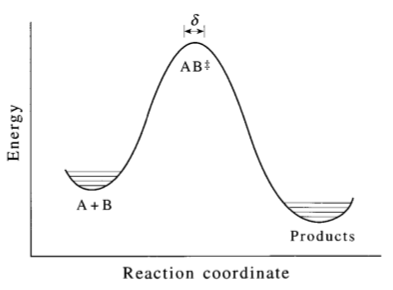
\includegraphics[width=0.75\textwidth]{figures/TST-PES.png}
    \caption[A reaction coordinate diagram for a generic reaction.]{A reaction
      coordinate diagram for the reaction of Equation \ref{eq:tst}. The TS complex is
      defined to exist in the small region $\delta$ above the reaction
      barrier. Figure taken from Reference {\protect\citenum{McQuarrie1997}}.}
    \label{fig:tst-pes}
\end{figure}

In TST, we define the TS complex to exist throughout a small region of width
$\delta$ above the reaction barrier (\ref{fig:tst-pes}). From the second step of
the reaction in Equation \ref{eq:tst}, we can define a reaction rate dependent
on the concentration $[\ch{AB}^\ddagger]$ and $v_c$, a factor which defines the
frequency with which the complexes proceed over the barrier:

\begin{equation}
  r = v_c [\ch{AB}^\ddagger]
\end{equation}

From Equations \ref{eq:a} and \ref{eq:tst}, we now have two equivalent
expressions for the reaction rate, which allows us to derive the following

\begin{equation}
  r = k[\ch{A}][\ch{B}] = v_c [\ch{AB}^\ddagger]
\end{equation}

\noindent and solving Equation \ref{eq:K} for $[\ch{AB}^\ddagger]$ results in


\begin{equation}
  r = v_c\frac{[\ch{A}][\ch{B}]K_c^\ddagger}{c^0}
\end{equation}

\noindent or

\begin{equation}
  k = \frac{v_cK_c^\ddagger}{c^0}
\label{eq:b}
\end{equation}

We must now invoke the statistical thermodynamics to make sense of Equation
\ref{eq:b}. We can rewrite the equilibrium expression $K_c^\ddagger$ in terms of
partition functions of each molecular species:

\begin{equation}
    K_c^{\ddagger} = \frac{[\ch{AB}^\ddagger]/c^0}{[\ch{A}]/c^0[\ch{B}]/c^0}
    = \frac{(q^\ddagger/V)c^0}{(q_A/V)(q_b/V)}
\label{eq:c}
\end{equation}

\noindent where $q_A$, $q_B$, and $q^\ddagger$ are the partition functions of A,
B, and AB$^\ddagger$, respectively.

Since we have defined the reaction to be occurring with one degree of freedom,
the translational partition function $q_{trans}$ can be defined as

\begin{equation}
  q_{trans} = \frac{\sqrt{2\pi m^\ddagger k_BT}}{h}\delta
\end{equation}

\noindent where $m^\ddagger$ is the mass of the TS complex. The partion function
of the TS complex can be written as the product $q^\ddagger =
q_{trans}q_{int}^\ddagger$, where the second term accounts for all remaining
degrees of freedom of the TS complex. We can use this and rewrite Equations
\ref{eq:c} and \ref{eq:b} as

\begin{equation}
  K_c^{\ddagger} =  \frac{\sqrt{2\pi m^\ddagger k_BT}}{h}\delta\frac{(q_{int}^\ddagger/V)c^0}{(q_A/V)(q_b/V)}
\end{equation}

\noindent and

\begin{equation}
 k = v_c \frac{\sqrt{2\pi m^\ddagger
     k_BT}}{hc^0}\delta\frac{(q_{int}^\ddagger/V)c^0}{(q_A/V)(q_b/V)}
\label{eq:d}
\end{equation}

We are now left with the two terms $v_c$ and $\delta$ which are
ill-defined. However, the product of these two terms is the average speed at
which the TS complex crosses the barrier, $\langle u_{TS} \rangle =
v_c\delta$. A Maxwell-Boltzmann distribution is used to calculate the value of
$\langle u_{TS} \rangle$:

\begin{equation}
  \langle u_{TS} \rangle = \left( \frac{m^\ddagger}{2\pi k_BT} \right)^{1/2}
  \int_0^\infty u e^{-m^\ddagger u^2/2k_BT}du = \left( \frac{m^\ddagger}{2\pi
      k_BT m^\ddagger} \right)^{1/2}
\label{eq:e}
\end{equation}

\noindent Substituting Equation \ref{eq:e} into Equation \ref{eq:d} for
$v_c\delta$ yields

\begin{equation}
  k =
  \frac{\sqrt{k_BT}}{hc^0}\frac{(q_{int}^\ddagger/V)c^0}{(q_A/V)(q_b/V)} = \frac{k_BT}{hc^0}K_c^\ddagger
\label{eq:f}
\end{equation}

Now, define the standard Gibbs free energy of activation
($\Delta ^\ddagger G^0$) to be the change in Gibbs free energy in going from
reactants to TS. The thermodynamical expression is

\begin{equation}
  \Delta ^\ddagger G^0 = -RT \ln K_c^\ddagger
\end{equation}

\noindent which can be substituted into Equation \ref{eq:f}

\begin{equation}
  k = \frac{k_BT}{hc^0} e^{-\Delta^\ddagger G^0/RT}
\label{eq:g}
\end{equation}

The standard Gibbs free energy of activation can be expressed in terms of
enthalpy and entropy as

\begin{equation}
  \Delta^\ddagger G^0 = \Delta^\ddagger H^0 - T \Delta^\ddagger S^0
\end{equation}

\noindent which, upon substitution gives the equation

\begin{equation}
  k = \frac{k_BT}{hc^0} e^{-\Delta^\ddagger S^0/R} e^{-\Delta^\ddagger H^0/RT}
\label{eq:M}
\end{equation}

At this point, we can draw a direct comparison to the Arrhenius equation
(Equation \ref{eq:arrhenius}) by expressing $E_a$ in terms of
$\Delta^\ddagger H^0$ and $A$ in terms of $\Delta^\ddagger S^0$.  We must
differentiate the natural logarithm of Equation \ref{eq:f}, as well as Equation
\ref{eq:arrhenius} (assuming that $A$ is independent of temperature):

\begin{equation}
  \frac{d \ln k}{dT} = \frac{1}{T} + \frac{d \ln K_c^\ddagger}{dT}
  \label{eq:h}
\end{equation}

\begin{equation}
  \frac{d \ln k_{Arr}}{dT} = \frac{E_a}{RT^2}
  \label{eq:i}
\end{equation}

\noindent Next, we use the fact that $d \ln K_c / dT = \Delta U^0/RT^2$ for an
ideal gas, then Equation \ref{eq:h}  becomes

\begin{equation}
  \frac{d \ln k}{dT} = \frac{1}{T} + \frac{\Delta ^\ddagger U^0}{RT^2}
  \label{eq:j}
\end{equation}

\noindent Additionally, $\Delta ^\ddagger H^0 = \Delta ^\ddagger U^0 + RT \Delta^\ddagger
n$ ($\Delta^\ddagger n = 1$), as so Equation \ref{eq:j} can be rewritten as

\begin{equation}
  \frac{d \ln k}{dT} = \frac{\Delta ^\ddagger H^0 + 2RT}{RT^2}
  \label{eq:k}
\end{equation}

\noindent Therefore, by comparison of Equation \ref{eq:k} and \ref{eq:i}, we get

\begin{equation}
  E_a = \Delta^\ddagger H^0 + 2RT
\end{equation}

\noindent which then converts Equation \ref{eq:M} into the form

\begin{equation}
  k = \frac{e^2k_BT}{hc^0}e^{\Delta^\ddagger S^0/R}e^{-E_a/RT}
\end{equation}

Therefore, a statistical thermodynamical picture of the Arrhenius equation
arises from TST, and the Arrhenius pre-factor $A$ can be expressed as

\begin{equation}
  A = \frac{e^2k_BT}{hc^0}e^{\Delta^\ddagger S^0/R}
\end{equation}

In practise, we use the form of Equation \ref{eq:g} to compute the rate constant
of a reaction, which we shall denote as $k_{TST}$. The conventional TST makes an
assumption that the reaction coordinate is static along the lowest energy
pathway. This can be corrected by the use of \emph{variational transition state
  theory}.\cite{Truhlar1984} We shall not consider variational TST in this work,
as with careful application, conventional TST does a remarkably good job at
accounting for the magnitude and temperature dependence of a wide range of
reactions.\cite{Steinfeld1998} Additionally, if one makes corrections for
\emph{QM tunnelling}, conventional TST can easily give a more complete
description of the rate constant.

\subsubsection{Quantum mechanical tunnelling}

Atoms are quantum mechanical particles, and are thus subject to the strange
probabilistic behaviours observed at the microscopic level. QM tunnelling refers
to the ability of particles to penetrate the reaction barrier, rather than
surmounting it classically (\ref{fig:tunnelling}). While all reactions are
subject to QM tunnelling, we will show that due to the low mass of the hydrogen
atom, QM tunnelling can play a significant role in HAT reactions.

\begin{figure}[htb]
  \centering
  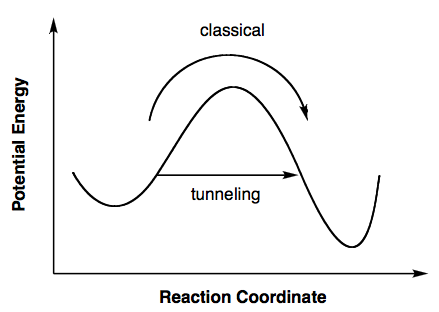
\includegraphics[width=0.7\textwidth]{figures/tunnelling}
  \caption{Quantum mechanical tunnelling occurs when a particle penetrates a
    reaction barrier, rather than surmounting it. \jnote{Place holder figure}}
  \label{fig:tunnelling}
\end{figure}


In order to determine the effects of scattering, one must find transmission
coefficients ($\kappa$) by solving the Schr{\"o}dinger equation. This is done by
approximating the reaction barrier with an analytical potential, thus
simplifying the problem mathematically. The earliest model potentials were
introduced by Bell, who used a parabolic function to approximate the reaction
barrier.\cite{Bell1980} To obtain $\kappa$, and thus the observed rate constant
($k_{obs}$), the following equations were used:

\begin{align}
  k_{obs} &= \kappa A e^{-E_a/RT}  \\
\kappa &= \frac{e^\alpha}{\beta-\alpha} \left(\beta e^{-\alpha} - \alpha
  e^{-\beta} \right) \\
  \alpha &= E_a/RT \\
  \beta &= \frac{2a\pi^2(2mE_a)^{1/2}}{h}
\end{align}

\noindent where the Arrhenius equation was used to estimate the rate constant,
$m$ is the mass of the tunnelling particle, and $2a$ is the width of the
barrier. Since the equation is dependent on the mass of the particle, tunnelling
occurs more often when lighter particles are involved. As a consequence,
tunnelling is more common in HAT reactions than other atom transfer
reactions. Also, the height and width of the barrier are important factors in
determining the contributions to tunnelling: reactions with small barriers have
low tunnelling contributions; narrow barriers result in higher tunnelling
contributions.

The Bell model is a poor representation of an actual reaction barrier. One which
is a much better approximation is the \emph{Eckart potential}.\cite{Johnston1962}
The form of this potential is

\begin{align}
  V &= -\frac{Ay}{1-y} - \frac{By}{1-y^2} \\
  y &= -e^{2\pi x/L}
\end{align}

\noindent where $x$ is the variable along the reaction coordinate and $L$ is
called the characteristic length. If $A=0$ the potential becomes a symmetric
function, further simplifying the problem; however, most reactions do not have a
symmetric potential. $A$, $B$ and $L$ are related to the change in barrier
height in the forward and reverse direction, $\Delta V1$ and $\Delta V_2$,
respectively:

\begin{align}
  A &= \Delta V_1 - \Delta V_2 \\
  B &= ((\Delta V_1)^{1/2} + (\Delta V_2)^{1/2})^2 \\
 \frac{L}{2\pi} &= (-\frac{2}{F^*})^{1/2} [\frac{1}{(\Delta V_1)^{1/2}} +
      \frac{1}{(\Delta V_2)^{1/2}}]^{-1}
\end{align}

\noindent where $F^* = d^2V/dx^2$ evaluated at the maximum of the potential. In
this formulation, $V$ is a placeholder energy. Note that if a reaction is
endoergic, tunnelling does not occur. Alteratively, one says tunnelling only
occurs in exoergic or energy-neutral reactions.

The solutions to the Schr{\"o}dinger equation for the Eckart potential are
analytical, thus that transmission coefficient $\kappa$ can easily be computed
using standard numerical techniques. These tunnelling corrections will be
applied, where applicable as

\begin{equation}
  k_{calc} = \kappa k_{TST} = \kappa
\frac{k_BT}{hc^0}e^{-\Delta^\ddagger G^0}
\end{equation}


%%% Local Variables:
%%% mode: latex
%%% TeX-master: "diss"
%%% End:


%%% !TEX root = diss.tex

\chapter{Methods}
\label{ch:methods}

In this chapter, we shall briefly outline the procedures and computational
methods used to obtain the results in this thesis. The methods have been broken
down in a per chapter manner. All quantum mechanical calculations were performed
using either the Gaussian 09\cite{Frisch2009} or TURBOMOLE
programs.\cite{turbomole} Molecular structures were built in the GaussView
program.\cite{gview} Optimised structures were verified local minima by
vibrational analysis and visualised using the Chemcraft program.\cite{ccraft}
Transition state structures were all verified saddle points by visualisation of
a single imaginary frequency connecting reactants to products. As a brief note
on notation, computational methods used are described using the following
notation: \emph{method}/\emph{basis}, for example, calculations performed using
the B3LYP density functional with 6-31+G* basis sets is denoted as
B3LYP/6-31+G*. Commonly, single-point energy calculations with a higher level of
theory (\emph{HL method} and \emph{HL basis}) are performed on structures
optimised with a lower level of theory (\emph{LL method} and \emph{LL basis}),
this is denoted as \emph{HL method}/\emph{HL basis}//\emph{LL method}/\emph{LL
  basis}. Thermochemical corrections are also taken from the lower level of
theory.

\section{Chapter \ref{ch:arrhenius}}

In this chapter, we seek to calculate pre-reaction complex binding energies for
bulky phenolic or peroxylic substrates which participate in nearly thermoneutral
reactions. Conformational analysis to locate the global minimum substrate
geometry was performed using the BLYP-D3(BJ)
method\cite{Becke1988,Lee1988,Grimme2010,Johnson2006} utilising the minimal
MINIs basis sets\cite{Huzinaga1984} and our groups own \emph{basis set
  incompletion potentials} (BSIPs).\jnote{citation needed} Geometries were
manipulated by manual rotation of the necessary dihedral bond angles, followed
by geometry optimisation and vibrational analysis.

The lowest energy substrates were combined to generate the appropriate
pre-reaction complexes. These pre-reaction complexes were subject to
conformational analysis using the same BLYP-D3(BJ)-BSIP/MINIs method. Geometries
were initially manipulated by hand. It became apparent that manual manipulation
resulted in an unsatisfactory exploration of the conformational space. To
overcome this, all the necessary dihedral angles were scanned systematically
using a combination of scripts.\cite{note5} All manipulated geometries were
subject to optimisation. For each complex, the top 5-10 complex geometries were
subject to further optimisation using a higher level of theory
(BLYP-D3(BJ)/pc-1) to obtain the final minimum energy pre-reaction complex
structures.\jnote{currently some non-minimum structures}

To obtain accurate pre-reaction complex binding energies, the substrates and
complexes were subject to single-point energy calculations using the
LC-$\omega$PBE long-range corrected density
functional\cite{Vydrov2006,Vydrov2006a} with D3(BJ) dispersion corrections and
pc-2 basis sets with truncated $f$-type functions (pc-2-spd).\cite{Johnson2013}
This method was selected on the recommendation of work by \citet{Johnson2013},
which demonstrated that this was an efficient method for calculation NCIs with a
reasonable degree of accuracy.

\section{Chapter \ref{ch:bde}}

In this chapter, we probe the applicability of the Bell-Evans-Polanyi principle
in two broad classes of C-H bond hydrogen atom transfer reactions with \cumo. In
order to do this, we seek to calculate BDEs which are \emph{chemically
  accurate}, that is, within 1 \kcalmol of the ``true value.'' To achieve this,
the highly accurate W1BD\cite{Barnes2009} quantum mechanical composite method
was employed.

Unfortunately, some of the substrates of interest are too large to be treated
with the W1BD method, thus we sought a less computationally expensive method
which most gave results of comparable precision. There is currenly no literature
which benchmarks computational procedures for bond dissociation enthalpies. As a
consequence, we explored a variety of other quantum mechanical composite
methods, including: the G4 and G4(MP2) methods,\cite{Curtiss2007,Curtiss2007a}
and the CBS-QB3, ROCBS-QB3, and CBS-APNO
methods.\cite{Montgomery1999,Montgomery2000,Ochterski1996}

\jnote{Is the LDBS approach relevant if we didn't use it for analysus in the
  end?}  Additionally, we developed a method which we call the \emph{locally
  dense basis set approach} (LDBS), which makes use of the ROCCSD(T) method with
a basis set partitioning scheme. The partitioning scheme is as follows: groups
which are close the the bond being broken are treated with large basis sets
(pc-3), while groups which are further away have incrementally smaller basis
sets. Specifically, we use a 3/2/1 partitioning, such that the carbons centred
group where bond dissociation occurs, as well as the groups immediately
adjacent, are treated with the high-level pc-3 basis sets. The next groups over
are treated with the medium-level pc-2 basis sets. Any groups beyond this are
treated with the low-level pc-1 basis sets. This is illustrated in
\ref{fig:ldbs}.


\begin{figure}[htb]
  \centering
  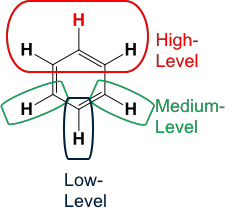
\includegraphics[width=0.6\textwidth]{figures/ldbs}
  \caption[Example locally dense basis set partitioning on benzene used in the
  LDBS approach.]{Example locally dense basis set partitioning on benzene used
    in the LDBS approach. The red hydrogen is that which is
    abstracted. High-level=pc-3, medium-level = pc-2, low-level = pc-1.}
  \label{fig:ldbs}
\end{figure}


The performance of all methods was compared to both the W1BD calculated BDEs, as
well as with experimentally available values, compiled from the \emph{Handbook
  of Bond Dissociation Energies}.\cite{Luo2002} Experimental values are obtained
using a wide variety of techniques, some of which may not be entirely
reliable. For example, thermochemical cycles\cite{Bordwell1988} are often used
to measure BDEs, however, this method has been shown to be unreliable if the
reaction used occurs by PCET rather than direct HAT.\cite{Miller2016} For this
reason, a secondary goal of this work is to identify any experimental BDEs which
may be in question.

To further probe the priniciples underlying the HAT reactions involved, TS
structures for the HAT reaction with \cumo have been obtained for a large number
substrates. TS structures were obtained using the B3LYP-D3(BJ)/6-31+G*
method. Where possible, TS structures were obtained for both a cisoid and
transoid conformation of the substrate/\cumo couple. Substrates and TS complexes
were subject to single-point energy calculations at the
LC-$\omega$PBE-D3(BJ)/6-311+G(2d,2p) level of theory to obtain more reliable
reaction barrier heights.

\section{Chapter \ref{ch:hat}}

In this chapter, we seek to understand the effects of non-redox active metal
cations of the hydrogen atom transfer reactions involving various organic
substrates with oxygen centred radicals. As shall be discussed in Chapter
\ref{ch:hat}, there is little literature which addresses the issue of
interactions between organic substrates and alkali and alkaline earth metals. To
address this, a benchmark study has been performed.

\subsection{Benchmark study of non-redox active metal cations with organic
  substrates}

The benchmark set shall be discussed in detail in Chapter \ref{ch:hat}. In order
to avoid erroneous charge transfer from the possible charge transfer involved in
cation-substrate interactions, conformational analysis was performed by manual
geometry manipulation using the LC-$\omega$PBE-D3(BJ)/6-31+G**
method.\cite{Johnson2013a} The most stable conformations of metal-substrate
complexes was subjected to higher-level optimisation at the
LC-$\omega$PBE-D3(BJ)/6-311+G(3df,3pd) level of theory.

Initially, binding energy for the metal-substrate complexes was calculated using
the full electron CCSD(T)/CBS approach, utilising two-point basis set
extrapolation with aug-pc-3 and aug-pc-4 basis sets. These results showed
systematic problems in the convergence of basis sets to the complete basis set
limit for the alkali and alkaline earth metals. To address this, the binding
energies were re-calculated using the full electron CCSD(T)-F12* explicitly
correlated approach\cite{Hattig2010} with Def2-QZVPPD basis sets.

A variety of DFT methods and basis sets were benchmarked against the
CCSD(T)-F12*/Def2-QZVPPD results (see Appendix \jnote{BLANK} for full
details). Single point energy calculations were performed on
LC-$\omega$PBE-D3(BJ)/6-311+G(3df,3pd) structures. The validity of these
structures was tested by re-optimisation with the three best performing DFT
methods relative to the benchmark data (M05-2X, BMK-D3(BJ), and $\omega$B97X-D
with large basis sets). The average root mean square deviation in geometry was
found to be onle 0.007-0.008 \AA ~for all three methods, thus validating the
structures. We elected to move forward using the M05-2X functional on the basis
of the results obtained from the benchmark study of metal cation-substrate
interactions, and the well described ability of M05-2X to accurately describe
HAT reactions involving oxygen centred radical.\cite{Galano2013}


\subsection{Effects of metal cations on hydrogen atom transfer barrier heights}



%%% Local Variables:
%%% mode: latex
%%% TeX-master: "diss"
%%% End:


% !TEX root = diss.tex

\chapter{The Relationship Between Arrhenius Pre-factors with Non-Covalent Binding}
\label{ch:arrhenius}

\section{Introduction}


DiLabio and Ingold\cite{DiLabio2005} previously investigated the formal HAT reaction of the iminoxyl/oxime self-exchange reaction. In that paper, they compiled a table of parameters from the phenomenological Arrhenius equation for a series of interesting reactions, which appear here in~\ref{tab:Arrhenius-expt}.\cite{Kreilick1966, Mader2004, Mahoney1970, DaRooge1967, Howard1973, Foti1994, Chenier1974, Chenier1975} These are thermoneutral hydrogen atom self-exchange reactions involving oxygen-centred $\pi$-radicals,\footnotemark\ and other nearly thermoneutral reactions involving the destruction and formation of oxygen-centred $\pi$-radicals, reactions 3.1 and 3.2, respectively:

\begin{align}
  \ch{$\pi$-RO^. + ROH &-> ROH + $\pi$-RO^.} \hspace{2cm} \Delta H = 0 \\
  \ch{$\pi$-R}^\prime\ch{O^. + ROH &-> R}^\prime\ch{OH + $\pi$-RO^.} \hspace{2cm} \Delta H \approx 0
\end{align}

\newcommand{\tabFig}[2][0.35]{\includegraphics[scale=#1]{figures/#2.eps}}

\begin{table}[!ht]
  \footnotesize
  \centering
  \caption[Table of results for (nearly) thermoneutral reactions studied.]{Table of results for (nearly) thermoneutral reactions studied. Units for $\Delta H$, $E_a$, and calculated binding energy (BE) are \kcalmol, $\log A$ are log \Ms, and $k$ are \Ms.\ References to the original literature are included with the Complex ID number. $^\dagger$Calculated binding energies involve structures which could not be fully optimized and contain one or more small imaginary frequencies. Adapted with permission from Reference \protect\citenum{DiLabio2005}. Copyright (2005) American Chemical Society.}
\begin{tabular}{l >{\centering}m{1.5cm} >{\centering}m{1.5cm} >{\centering}m{1.2cm} >{\centering}m{1.2cm} >{\centering}m{1.2cm} >{\centering}m{1.2cm} >{\centering}m{0.8cm} m{0em}}
  ID & \ch{RO^.}/\ch{R}$^\prime$\ch{O^.} & \ch{ROH} & $\Delta H$ & $\log~A$ & $E_a$ & $k$ & BE & \\
  \toprule
  1\cite{Kreilick1966} & \tabFig{3tBuPhO} & \tabFig{3tBuPhOH} & 0.0 & 3.7 & 1.2 & 3.3\E{2} & -10.8 &\\
  2\cite{Mader2004} & \tabFig{4MeC5H4ONO} & \tabFig{4MeC5H6NOH} & -2.0 & 3.8 & 3.8 & 10 & -14.8 &\\
  3\cite{Kreilick1966}$^\dagger$ & \tabFig[0.4]{2tBuNO} & \tabFig[0.4]{2tBuNOH} & 0.0 & 5.1 & 3.5 & 3.3\E{2} & -10.1 &\\
  4\cite{Mahoney1970,DaRooge1967}$^\dagger$ & \tabFig{3tBuPhO} & \tabFig{tBuPhOH} & 4.2 & 5.5 & 4.8 & 93 & -10.0 &\\
  5\cite{Howard1973} & \tabFig[0.7]{tBuOO} & \tabFig{3tBuPhOH} & -7.0 & 4.2 & 0.5 & 7\E{3} & -6.5 &\\
  6\cite{Kreilick1966}$^\dagger$ & \tabFig[0.7]{Ph2NO} & \tabFig[0.7]{Ph2NOH} & 0.0 & $>$7 & - & $>$10$^7$ & -13.6 &\\
  7\cite{Foti1994} & \tabFig{PhO} & \tabFig{2hydroxynaphthalene} & -2.2 & 8.3 & 2.3 & 4\E{6} & -8.6 &\\
  8\cite{Chenier1974}$^\dagger$ & \tabFig[0.7]{tBuOO} & \tabFig{PhOH} & 0.3 & 7.2 & 5.2 & 3\E{3} & -5.5 &\\
  9\cite{Chenier1974}$^\dagger$ & \tabFig[0.7]{tBuOO} & \tabFig{2hydroxynaphthalene} & -1.9 & 6.4 & 2.6 & 3\E{4} & -5.6 &\\
  10\cite{Chenier1975}$^\dagger$ & \tabFig[0.7]{tBuOO} & \tabFig{alphatetralinperoxide} & 1.4 & 6.0 & 4.5 & 7\E{2} & -8.0 &
\end{tabular}
\label{tab:Arrhenius-expt}
\end{table}

\footnotetext{\noindent A $\pi$-radical is one in which the SOMO is orthogonal to the plane of the molecular framework, i.e.\ of $\pi$-symmetry. Note that free alkoxyl radicals cannot be distinguished as either $\sigma$ or $\pi$-radicals, as the SOMO is degenerate, or free to rotate with respect to the rest of the molecular framework. Therefore, only the geometry of the radical-molecule complex can resolve the symmetry of the SOMO.}

Although it is well known that reactions of this nature involve remarkably low activation energies ($E_a$),\cite{Lucarini1996, Mahoney1970a, Mahoney1975, Korcek1972} they also have unusually low Arrhenius pre-exponential factors ($A$), or as they shall be referred to herein, \emph{A-factors}. As a result, these reactions are generally slower than expected, evidence for which is summarized in~\ref{tab:Arrhenius-expt}: The measured A-factors are small, and range from $10^{3.5}$--$10^{8.3}$ \Ms.\
In the past, this has been attributed to steric shielding around the oxygen atoms, resulting in a large entropic barrier.\cite{DiLabio2005} Importantly, it was noted that the degree of steric shielding on the oxygen atom appears to play an important role in the order of the A-factor; systems with greater bulk have lower A-factors, while non-shielded systems have larger A-factors.

Stereo-electronic effects are known to play an important role in HAT, and have been studied extensively.\cite{Finn2004, Salamone2011, Pischel2001, Griller1981, Bietti2011, Salamone2012, Malatesta1982, Salamone2014} Although the abstraction of a specific hydrogen atom may be more thermodynamically favourable than others on a given substrate, if it is not accessible due to steric constraints, abstraction will not occur at this site. Otherwise, additional steric bulk can lead to significant reductions in reactivity, through destabilization of the TS complex, or by forcing additional processes involving conformational changes in order to reach the appropriate TS structure. For example, in reactions of tertiary acetamides with \cumo,\cite{Salamone2014} where abstraction occurs mainly from C-H bonds $\alpha$ to the nitrogen atom, a two-fold decrease in the rate constant (normalized for the number of equivalent hydrogen atoms) is observed in going from $N,N$-dimethylacetamide to $N,N$-diisobutylacetamide ($k_H$ = $2.0 \times 10^5$ and $7.8 \times 10^4$ \Ms, respectively). The decrease in rate constant is attributed to the steric clash between the methyl groups of \cumo\ and the isobutyl groups of $N,N$-diisobutylacetamide.

Upon first inspection, all of the reactions in~\ref{tab:Arrhenius-expt} appear to be of a similar nature. Each reaction involves the breaking and formation of O-H bonds as the thermodynamic driving force. All of these bonds are expected to be of comparable strength, therefore, differences should not contribute significantly to reaction barriers in a Bell-Evans-Polanyi principle fashion. Hence, the large degree of variance in their rate constants ($k$) is somewhat surprising. These reactions are closely related to the self-exchange reaction between phenol and phenoxyl,\cite{Mayer2002} in which a strong molecule-radical pre-reaction complex is formed, ca. 10 \kcalmol\ below the separated reactants. It is therefore expected that most, if not all, of the systems in~\ref{tab:Arrhenius-expt} should exhibit a similar molecule-radical complex; granted, the strength of the interaction will vary because of steric repulsion.

Currently, there has been no comprehensive investigation of the relationship between the pre-reaction complex and the kinetics of a reaction. Using the reactions and data in~\ref{tab:Arrhenius-expt}, we ask the question: \emph{Do A-factors have a correlation with non-covalent binding energies of the pre-reaction complex?} This is a reasonable question as non-covalent binding and steric hinderance represent a loss of degrees of freedom and therefore entropy,\footnotemark\ which ultimately determines the A-factor magnitude. If the answer to the question is yes, then non-covalent binding may be useful as a diagnostic for the ``looseness'' or ``tightness'' of a TS complex, in addition to providing an important link between theory and experiment.

\footnotetext{Recall from Equation~\ref{eq:afactor} that the A-factor can be related to TST such that the primary variable is entropy ($\Delta^\ddagger S^0$).}

\section{Computational methods and details}

Density-functional theory (DFT) calculations were carried out using the Gaussian-09 software package.\cite{Frisch2009} Care was taken to obtain minimum energy structures through detailed conformational analysis. For this, the BLYP density-functional\cite{Becke1988,Lee1988} was utilized, paired with the empirical D3 dispersion correction\cite{Grimme2010} with the recommended Becke-Johnson damping functions,\cite{Johnson2006} as well as our groups' own basis set incompletion potentials (BSIPs),$^*$\jnote{update citation} and minimal MINIs basis sets.\cite{Huzinaga1984} The use of minimal basis sets corrected for basis set incompleteness allows DFT-based methods (as opposed to semi-empirical or force-field based approaches) to be used efficiently in performing a large number of calculations. Minimum energy conformers of the monomers (substrates and radicals) were first obtained by manual manipulation of the necessary dihedral bond angles, followed by geometry optimization and vibrational analysis.

The lowest energy radicals and substrates were combined to generate the appropriate pre-reaction complexes. These pre-reaction complexes were subject to conformational analysis using the same BLYP-D3(BJ)-BSIP/MINIs method. Geometries were initially manipulated by hand. It became apparent that manual manipulation resulted in an unsatisfactory exploration of the conformational space. To solve this, all the necessary dihedral angles were scanned systematically using a combination of scripts.\bibnote{The Escher program\cite{escher} was used to generate a Z-matrix with specific dihedral angles. This geometry was then systematically scanned using simple shell scripts.} All manipulated geometries were subject to optimization. For each complex, the top 5--10 complex geometries were subject to further optimization using a higher level of theory (BLYP-D3(BJ)-BSIP/pc-1) to obtain the final minimum energy pre-reaction complex structures. Due to the free rotation of groups such as $t$-butyl and methyl, some of the optimized pre-reaction complex structures contain small imaginary frequencies, and thus do not represent proper stationary states. Several measures were taken to resolve this, however, no resolution was obtained in many cases. Regardless, the complexes adequately represent the pre-reaction complex and differences in ``true'' binding energies can likely be ignored.

To obtain accurate pre-reaction complex binding energies, the substrates and complexes were subject to single-point energy calculations using the LC-$\omega$PBE long-range corrected density functional\cite{Vydrov2006,Vydrov2006a} with D3(BJ) dispersion corrections and pc-2 basis sets with truncated $f$-type functions (pc-2-spd).\cite{Johnson2013} This method was selected on the recommendation of work by \citet{Johnson2013}, which demonstrated the accuracy of this method for the calculation of NCIs. On the basis of the reported mean absolute error in Reference \citenum{Johnson2013} for the S66 benchmark set of sixty-six different non-covalently interacting dimers,\cite{Rezac2011} the calculated binding energies reported herein from the LC-$\omega$PBE-D3(BJ)/pc-2-spd level of theory carry an estimated 0.2 \kcalmol\ margin of error.

\section{Results and discussion}

The theoretically determined electronic binding energies calculated for the lowest energy pre-reaction complex of each system are listed in~\ref{tab:Arrhenius-expt}. The logarithm of A-factor against binding energy was plotted, as shown in~\ref{fig:Arrhenius}. The overall correlation is quite poor ($R^2$ = 0.33), however much of the data is grouped about a single, well correlated line ($R^2$ = 0.95). The intercept of the fitted line which corresponds to zero binding energy is 8.63, a value which is in line with what has been cited as the expected A-factor for HAT reactions, \emph{viz. }$10^{8.5\pm0.5}$ \Ms.\cite{Benson1976} These results suggest that the observed correlation is genuine, that is, NCIs may have an impact on A-factors. I shall demonstrate that the data which do not correlate are reasonable outliers. In fact, using simple rationale I shall demonstrate that different regimes of steric bulk results in different processes leading to the TS complex. As a result, deviations from the relationship between A-factor and binding energy are observed.

\begin{figure}[!htbp]
  \centering
  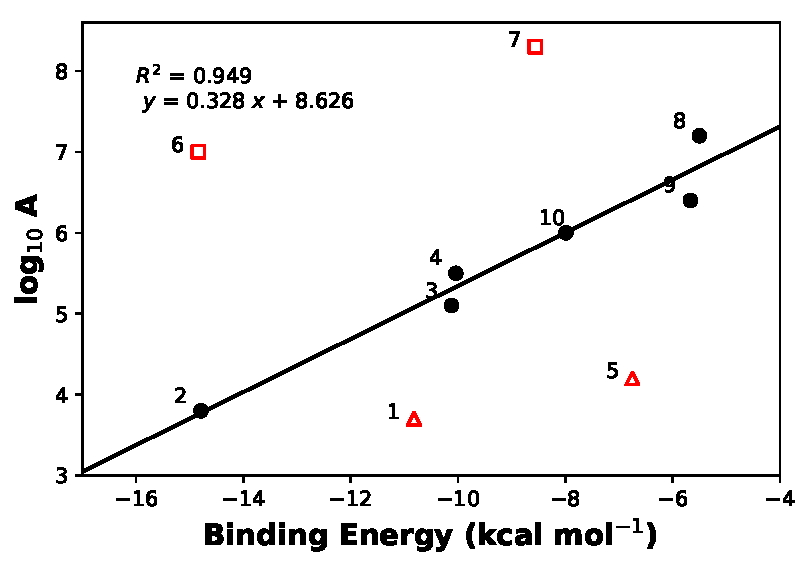
\includegraphics[width=0.85\textwidth]{figures/arrhenius-scatter.pdf}
  \caption[Plot of logarithm of A-factor against binding energy.]{Plot of logarithm of A-factor against binding energy. Only the black points were included in the line fitting (slope = 0.328 \kcalmol, intercept = 8.626 \kcalmol, and $R^2$ = 0.949). Red points with open faced markers indicate outliers, \emph{vide infra}. The inclusion of complexes 1, 5, and 7 result in an $R^2$=0.334. Complex 6 is always omitted from line fitting as the experimental A-factor is approximate.}
\label{fig:Arrhenius}
\end{figure}

In order to illustrate this, consider the fundamental properties of the HAT reactions involved herein. There are two important concerted reaction mechanisms that are possible, namely direct HAT or PCET.\@ Specifically, we must consider the geometric constraints in which these reaction mechanisms occur. For direct HAT to occur, the SOMO of the radical must overlap with the O-H $\sigma^*$ anti-bonding orbital. This may require the rotation of the hydrogen atom donating hydroxyl group out of the plane. The rotation of a phenolic hydroxyl group has an energy barrier that follows a $\cos^2 \theta$ relationship,\cite{Kojima1960} and can be as high as 3.1 \kcalmol\ on the basis of the rotational barrier in phenol.\cite{Kim1994} For a PCET mechanism to occur, there are two possible geometries: Either the SOMO of the radical overlaps can overlap with the corresponding oxygen lone pair $p$-orbital, as seen in the work of \citet{Mayer2002}; or a lone pair-$\pi$ or $\pi$-$\pi$ bonding overlap between the radical and substrate can occur, as seen in the work of \citet{DiLabio2007}. Due to time constraints, I did not seek to obtain TS complex structures. Nonetheless, from the pre-reaction complex one can surmise the most likely TS complex. Thus, by applying these basic principles, it is possible to rationalize deviations from the trend observed in~\ref{fig:Arrhenius}.

\begin{figure}[!htbp]
\centering
\hspace*{-1.8cm}
\begin{minipage}{8cm}
  \centering
  \begin{overpic}[width=\textwidth]{figures/complex2_hbond}
  \put(5,91) {\large\textbf{A.}}
\end{overpic}
\end{minipage}%
\begin{minipage}{8cm}
  \centering
  \begin{overpic}[width=\textwidth]{figures/complex3_hbond}
  \put(5,90) {\large\textbf{B.}}
\end{overpic}
\end{minipage}
\caption[Three-dimensional structures of pre-reaction complexes 2 (TEMPO-H and 4-oxo-TEMPO) and 3 (di-$t$-butyl-hydroxylamine and di-$t$-butyl-nitroxyl).]{Three-dimensional structures of \textbf{A} complex 2, and \textbf{B} complex 3. Hydrogen bond distances are shown in units of \AA.\@ The elements are coloured as white for carbon, light blue for hydrogen, red for oxygen, and blue for nitrogen.}
\label{fig:com2-3}
\end{figure}

We shall begin by examining the points which fall on the expected line, complexes 2--4 and 8--10. The examination of all these pre-reaction complexes reveals that an additional process that has a moderate energetic barrier is required in order for formal HAT reactions to proceed. Complexes 2 and 3 are shown in~\ref{fig:com2-3}, and are very similar in structure. Both are hydroxylamine-nitroxyl couples with similar degrees of steric bulk adjacent to the reacting centres. The $t$-butyl groups of 3, and the methyl groups of 2 prevent the alignment of the NO-H-ON frameworks in a PCET manner. In order to reach the TS complex, both 2 and 3 must bring methyl groups within close proximity for direct HAT to occur. In the most stable stacked conformation, complex 4, as seen in~\ref{fig:com4}, cannot undergo PCET as the steric clash of the para-position $t$-butyl groups prevent $\pi$-$\pi$ overlap. In order to react via direct HAT, the hydroxyl group must rotate further out of the aromatic plane, or the bulky para-position $t$-butyl groups must come into close proximity. Alternatively, an open conformation for complex 4 is possible, which lies ca. 2 \kcalmol\ higher in energy than the stacked complex, a result which is also consistent with the observed trend-line. From the open conformation, PCET is still not possible due to the steric bulk of the ortho-position $t$-butyl groups of the radical, thus this reaction likely proceeds through a direct HAT mechanism.

\begin{figure}[!htbp]
\centering
\hspace*{-1.8cm}
\begin{minipage}{8cm}
  \centering
  \begin{overpic}[width=\textwidth]{figures/complex4_hbond}
  \put(10,110) {\large\textbf{A.}}
\end{overpic}
\end{minipage}%
\begin{minipage}{8cm}
  \centering
  \begin{overpic}[width=\textwidth]{figures/complex4_steric}
  \put(0,105) {\large\textbf{B.}}
\end{overpic}
\end{minipage}
\caption[Three-dimensional structure of pre-reaction complex 4 between 2,4,6-tri-$t$-butylphenol and  4-$t$-butylphenoxyl.]{Three-dimensional structure of pre-reaction complex 4 between 2,4,6-tri-$t$-butylphenol and  4-$t$-butylphenoxyl. \textbf{A} demonstrates the hydrogen bond distances in units of \AA, and the out-of-plane rotation by 35.2$^\circ$ of the phenolic hydroxyl group. \textbf{B} demonstrates the steric clash (highlighted by red box) between the para-position $t$-butyl groups. The elements are coloured as white for carbon, light blue for hydrogen, and red for oxygen.}
\label{fig:com4}
\end{figure}

Complexes 8 and 9 are similar systems, in which \ch{$t$-BuOO^.} reacts with unhindered phenolic substrates. As seen by the structures in~\ref{fig:com8-9}, the bound complexes are somewhat dissimilar. The hydroxyl group of complex 8 is rotated out of the plane 24$^\circ$, while in complex 9 the hydroxyl group lies entirely in the plane. It is likely that the larger aromatic system of 2-naphthol results in a larger OH rotational barrier, and thus the most favourable conformation is entirely in the plane. Complex 8 was previously studied by \citet{DiLabio2007}, where it was demonstrated that a partial bonding interaction exists between the peroxyl lone-pair and phenolic $\pi$-system, and thus formal HAT proceeds through a PCET mechanism. Although the pre-reaction complexes are somewhat dissimilar, the conformational changes necessary to reach a PCET TS complex, similar to that reported in reference \citenum{DiLabio2007}, are likely not dramatically different in terms of energetic barriers. Any small differences result in noise in the observed trend.

\begin{figure}[!htbp]
\centering
\hspace*{-1.8cm}
\begin{minipage}{8cm}
  \centering
  \begin{overpic}[width=\textwidth]{figures/complex8_hbond}
  \put(0,110) {\large\textbf{A.}}
\end{overpic}
\end{minipage}%
\begin{minipage}{8cm}
  \centering
  \begin{overpic}[width=\textwidth]{figures/complex9_hbond}
  \put(0,100) {\large\textbf{B.}}
\end{overpic}
\end{minipage}
\caption[Three-dimensional structures of pre-reaction complexes 8 ($t$-butylperoxyl and phenol) and 9 ($t$-butylperoxyl and 2-naphthol).]{Three-dimensional structures of pre-reaction complexes \textbf{A.} 8 ($t$-butylperoxyl and phenol) and \textbf{B.} 9 ($t$-butylperoxyl and 2-naphthol). Hydrogen bond distances are shown in units of \AA.\@ Complex 8 has an out of plane rotation of the phenolic hydroxyl group of 24.1$^\circ$. The elements are coloured as white for carbon, light blue for hydrogen, and red for oxygen.}
\label{fig:com8-9}
\end{figure}

Complex 10 is unique in that it is the only reaction between a peroxide and a peroxyl radical. The self-exchange reaction between \ch{HOO^.} and \ch{HOOH} can be considered the simplest reference for the reaction of $\alpha$-tetralin peroxide with $t$-butylperoxyl. To the best of my knowledge, the mechanism of the hydroperoxyl-hydrogen peroxide couple has not been characterized as either PCET or direct HAT previously in the literature, although the TS structure has been previously reported.\cite{Isborn2005} Using this structure, calculations reveal a lone pair-lone pair interaction leading to partial bonding in the TS, i.e.\ a PCET mechanism. (See Appendix~\ref{ap:arrhenius},~\ref{fig:hooh-ooh}). Also the hydroperoxyl-hydrogen peroxide couple appears to prefer an \ch{H-O-O-H} dihedral angle of 90$^\circ$, so that the two non-reacting hydrogen atoms oriented 180$^\circ$ away from one another. Orienting substituents directly away from one another is likely the most stable TS structure for all peroxyl-peroxide formal HAT reactions. In order for complex 10 to achieve a similar TS structure, $t$-butylperoxyl and $\alpha$-tetralin peroxide must reorganize to avoid steric clash, likely through a rotation of the \ch{HOO} moiety of $\alpha$-tetralin peroxide.

\begin{figure}[!htbp]
\centering
\hspace*{-1.8cm}
\begin{minipage}{8cm}
  \centering
  \begin{overpic}[width=\textwidth]{figures/complex10_hbond}
  \put(0,100) {\large\textbf{A.}}
\end{overpic}
\end{minipage}%
\begin{minipage}{8cm}
  \centering
  \begin{overpic}[width=\textwidth]{figures/complex10_steric}
  \put(0,100) {\large\textbf{B.}}
\end{overpic}
\end{minipage}
\caption[Three-dimensional structure of pre-reaction complex 10 between $t$-butylperoxyl and $\alpha$-tetralin peroxide.]{Three-dimensional structure of pre-reaction complex 10 between $t$-butylperoxyl and $\alpha$-tetralin peroxide. \textbf{A} demonstrates the hydrogen bond distances in units of \AA. \textbf{B} demonstrates the incorrect orientation of the peroxyl-peroxide units for a PCET TS complex to occur. The elements are coloured as white for carbon, light blue for hydrogen, and red for oxygen.}
\label{fig:com10}
\end{figure}

Once again, complexes 2--4 and 9--10 follow the observed trend. In all cases, these complexes must undergo an additional conformational change with a small energy barrier in order to reach the pre-reaction complex which leads directly to the TS complex. This is illustrated in~\ref{fig:afactor-trend},

\begin{figure}[!htbp]
  \centering
  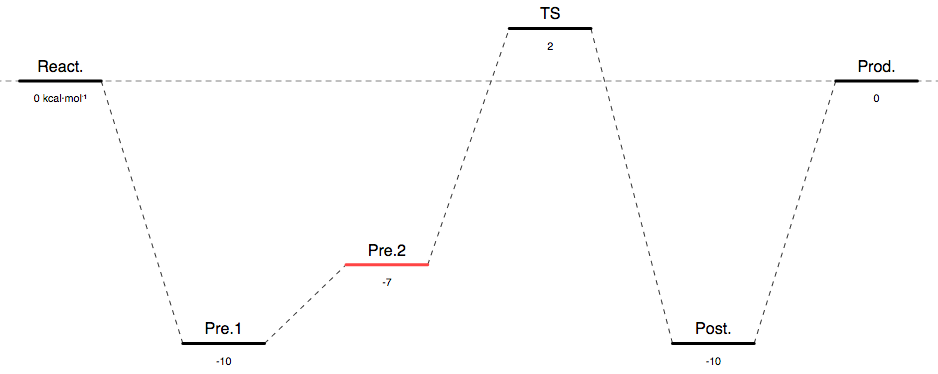
\includegraphics[width=\textwidth]{figures/afactor-trend.png}
  \caption[Reaction coordinate illustrating a conformational change to a second pre-reaction complex prior to transition state formation.]{Reaction coordinate illustrating a conformational change to a second pre-reaction complex prior to transition state formation. Energies are estimated for a self-exchange reaction. React. = reactants, Pre.1 = lowest energy pre-reaction complex, Pre.2 = postulated higher energy pre-reaction complex involving conformational change, TS = transition state, Post. = post-reaction complex, Prod. = products.}
\label{fig:afactor-trend}
\end{figure}

Consider next the points which sit above the trendline, complexes 6 and 7. The A-factor for complex 6 is approximate and thus does not get factored into the line fitting. In both cases, the non-covalently bound complexes are in a slipped-parallel $\pi$-stacked conformation. Complex 7 in particular is very similar to the phenol-phenoxyl couple, except with 2-naphthol instead of phenol. Therefore, it is possible to infer that both of these reactions take place through a PCET mechanism. In fact, these pre-reaction complexes are optimally aligned to achieve the appropriate TS complexes. Therefore, in contrast to the observed trend, complexes 6 and 7 do not require an additional conformational change to approach the TS complexes, as illustrated in~\ref{fig:afactor-direct}.

\begin{figure}[!htbp]
  \centering
  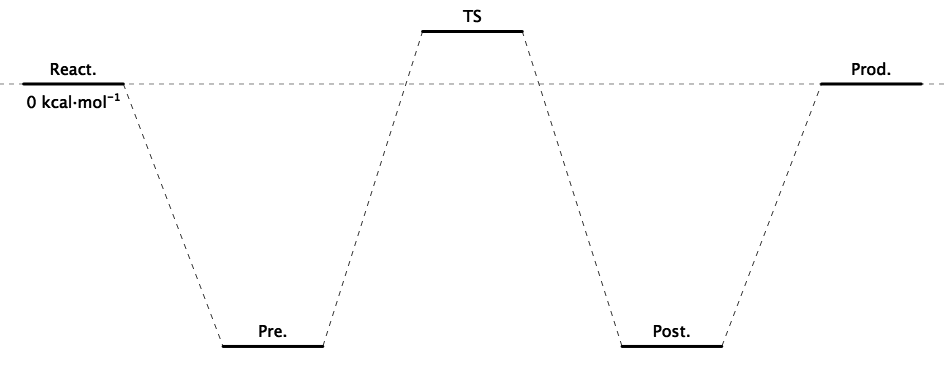
\includegraphics[width=\textwidth]{figures/afactor-direct.png}
  \caption[Reaction coordinate illustrating no conformational change before moving from pre-reaction complex to the transition state.]{Reaction coordinate illustrating no conformational change before moving from pre-reaction complex to the transition state. Energies are estimated based on a self-exchange reaction. React. = reactants, Pre. = lowest energy pre-reaction complex, TS = transition state, Post. = post-reaction complex, Prod. = products.}
\label{fig:afactor-direct}
\end{figure}

Lastly, consider the points which fall below the trendline, complexes 1 and 5. In both cases, a high degree of steric repulsion likely does not allow for a PCET mechanism. Complex 1 is the self-exchange reaction between the very bulky 2,4,6-tri-$t$-butylphenol-2,4,6-tri-$t$-butylphenoxyl couple, as seen in~\ref{fig:com1-5} A. As a result of steric shielding around the reaction centres, the most stable pre-reaction complex is stacked to maximize dispersion interactions, but does not have a hydrogen bond, which is unique among the ten reaction couples studied herein. Therefore, these must be a higher-energy hydrogen-bonded pre-reaction couple that leads to the HAT transfer. Note however, that there is a barrier to rotation of the hydroxyl group to 90$^\circ$ out of the plane for direct HAT to occur.

\begin{figure}[!htbp]
\centering
\hspace*{-1.8cm}
\begin{minipage}{8cm}
  \centering
  \begin{overpic}[width=\textwidth]{figures/complex1}
  \put(0,100) {\large\textbf{A.}}
\end{overpic}
\end{minipage}%
\begin{minipage}{8cm}
  \centering
  \begin{overpic}[width=\textwidth]{figures/complex5_new}
  \put(0,100) {\large\textbf{B.}}
\end{overpic}
\end{minipage}
\caption[Three-dimensional structures of pre-reaction complexes 1 (2,4,6-tri-$t$-butylphenoxl and 2,4,6-tri-$t$-butylphenoxyl) and 5 (2,4,6-tri-$t$-butylphenol and $t$-butylperoxyl).]{Three-dimensional structures of pre-reaction complexes \textbf{A.} 1 (2,4,6-tri-$t$-butylphenoxl and 2,4,6-tri-$t$-butylphenoxyl) and \textbf{B.} 5 (2,4,6-tri-$t$-butylphenol and $t$-butylperoxyl. Distances in unit of \AA and angles are shown in degrees. The elements are coloured as white for carbon, light blue for hydrogen, and red for oxygen.}
\label{fig:com1-5}
\end{figure}

Complex 5 is the 2,4,6-tri-$t$-butylphenol-$t$-butylperoxyl reaction couple. The lowest-energy pre-reaction complex contains a hydrogen bond, however the hydroxyl group is rotated 90$^\circ$ out of the plane. It is likely that as with complex 1, a pre-reaction complex without a hydrogen bond forms first. However, in complex 1 there is less steric clashing, thus the formation of a hydrogen bond is favourable. There is a barrier to rotation\footnotemark\ of the hydroxyl group that is about 4.1 \kcalmol. Note the unusual character of the hydrogen bond formed. Optimal hydrogen bonds are nearly linear so that there is both a dipole-dipole interaction and an orbital interaction such that the lone pair of the acceptor donates electron density into the OH $\sigma^*$ anti-bonding orbital.\cite{Jeffrey1997} In the case of complex 5, the hydrogen bond is nearly perpendicular, resulting in only an orbital interaction.\footnotemark\ The lowest energy pre-reaction complex 5 is comparable to that of complex 8, the TS of which as published in reference \citenum{DiLabio2007}. Formal HAT in complex 8 takes place through a PCET mechanism, however due to steric shielding it is unlikely that the correct $\pi-\pi$ orbital overlap can occur for PCET to occur. Therefore, this reaction can also be described as taking place through a direct HAT mechanism.

\footnotetext{Calculated as the difference in energy between the in-plane and out-of-plane structures of 2,4,6-tri-$t$-butylphenol at the LC-$\omega$PBE-D3/6-311+G(2d,2p) level of theory.}

\footnotetext{The hydrogen bonding nature of this interaction has been verified using the NCIplot software.\cite{Johnson2010,ContrerasGarcia2011} These results can be found in Appendix~\ref{ap:arrhenius},~\ref{fig:nciplot}.}

Complexes 1 and 5 fall below the trendline of $\log A$ vs calculated binding energy. Because of the steric bulk of 2,4,5-tri-$t$-butylphenol, the hydroxyl group must rotate $90^\circ$ out of plane from the minimum energy structure,  in order for HAT to occur. This process has an energy barrier of about 4.1 \kcalmol. For complex 1, this results in a higher energy pre-reaction complex, while for complex 5 this results in a lower energy pre-reaction complex. However, because the formation of a non-hydrogen bonded complex must necessarily come first, the experimental A-factor does not correlate with the calculated binding energy as observed for complexes 2--4 and 8--10, which undergo a conformational change with little or no barrier. That is to say, the rotation of the phenol hydroxyl group is an additional process with a significant energy barrier, and thus explains the difference in trends.

\section{Summary}

In this investigation, I report the lowest energy pre-reaction complexes for a series of thermoneutral or nearly thermoneutral HAT reactions. I have plotted the theoretically determined electronic binding energies against the logarithm of experimentally determined A-factors. These results demonstrate that the A-factor is correlated to some extent with the binding energy, given that the reactions proceed through energetically similar pathways. The results herein can be sorted into three bins:

\begin{enumerate}
  \item Complexes which require a small conformational with no barrier to approach the TS structure fall onto the observed trendline. This appears to be the most likely case for formal HAT reactions.

  \item Complexes which are optimally aligned to approach the TS structure. This was the case for complexes 6 and 7.

  \item Complexes which the full $90^\circ$ rotation of the phenolic hydroxyl group is required for formal HAT to occur. This is the case when the phenol is highly sterically shielded.
\end{enumerate}

These results indicate that different regimes of steric interactions lead to different chemical processes in seemingly similar reactions. As a results, non-covalent binding can be used as a metric for kinetics parameters, however, it cannot full describe the entropic factors which contribute to the A-factor. One must first determine the relationship between the pre-reaction and TS complex.

Additional work is necessary to extend these results. In particular, a larger sample of data points should be used. Regardless, the results herein represent a novel attempt to link theory and experiment. Given that obtaining the full PES for large molecules is currently computationally impractical, these results serve as a seed for developing a fundamental understanding of complex formal HAT reactions.


% !TEX root = diss.tex

\chapter{Interrogation of the Bell-Evans-Polanyi Principle: Investigation of the Bond Dissociation Enthalpies correlated with Hydrogen Atom Transfer Rate Constants}
\label{ch:bde}

\section{Introduction}

The Bell-Evans-Polanyi (BEP) principle is a conceptual framework that states, for two closely related reactions, the difference in activation energy is proportional to the difference in their enthalpy of reaction.\cite{Bell1936,Evans1938,Dill2003} This is commonly expressed as the linear free energy relationship (LFER): $E_a = E_0 + \alpha \Delta H$ (Equation~\ref{eq:bep}). Initially, the BEP principle was used as a simple model to explain the Br{\o}nsted catalysis law, which states that the stronger and acid is, the faster the catalysed reaction will proceed.\cite{Bronsted1924} A key assumptions is made for the BEP principle: the position of the TS along the reaction coordinate is the same for all reactions. The relationship can be described schematically: the more stable the product, the lower the reaction barrier, as seen in~\ref{fig:bep}.

\begin{figure}[!htbp]
  \centering
  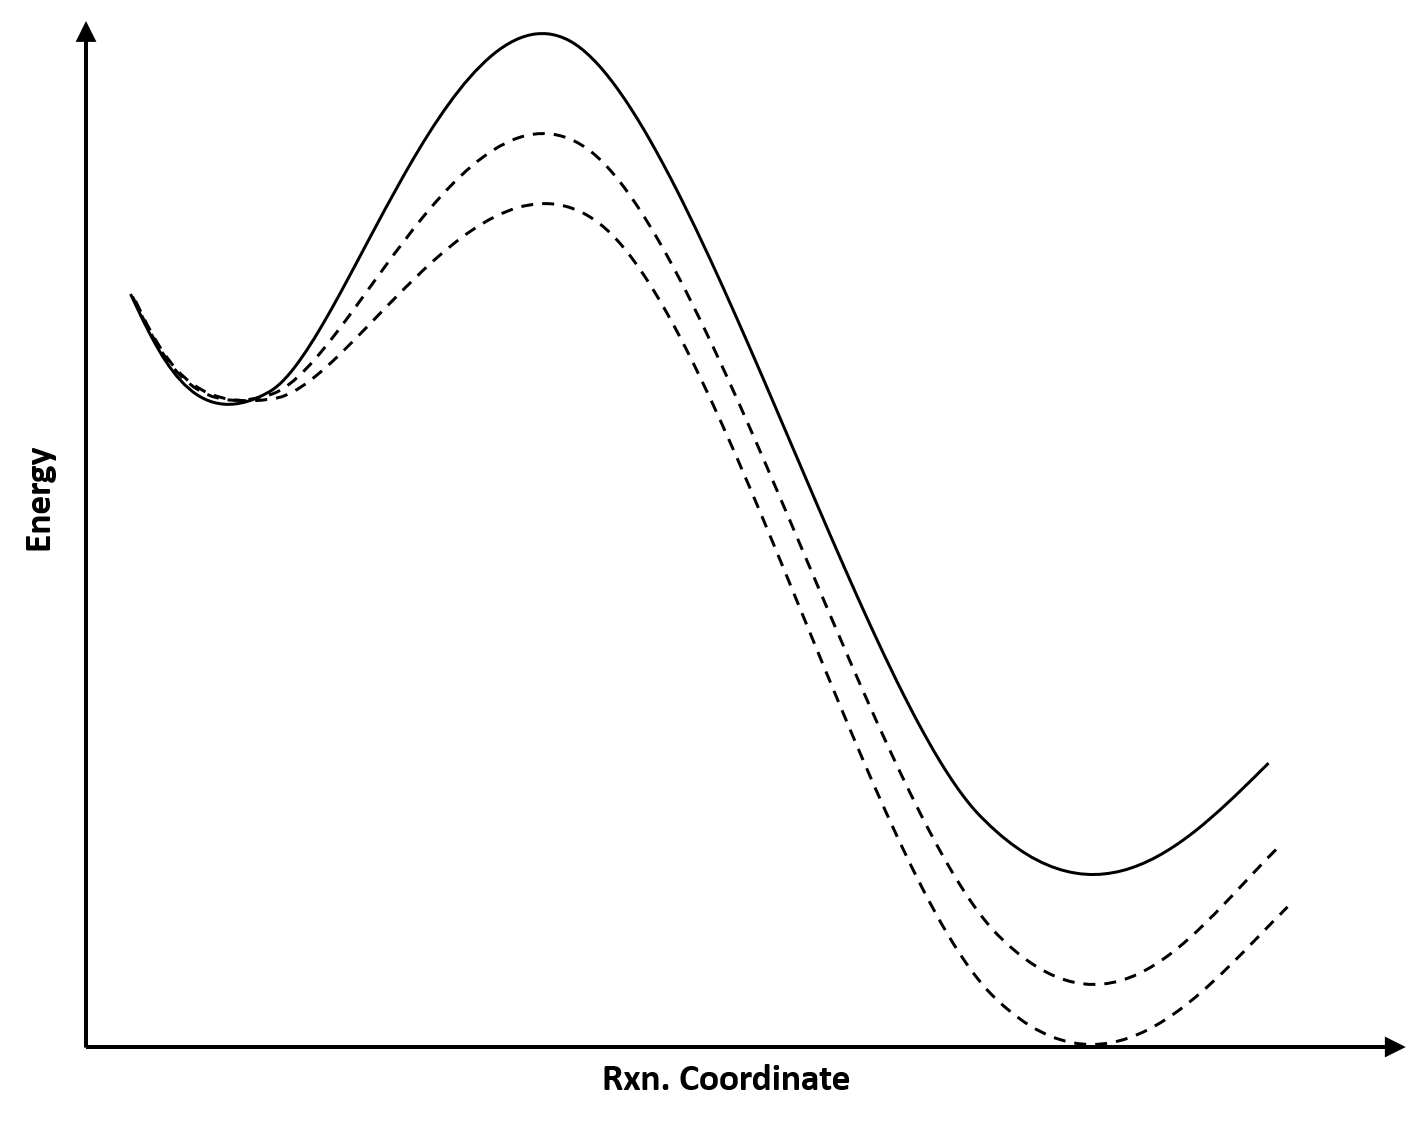
\includegraphics[width=0.7\textwidth]{figures/bep}
  \caption{Energy profiles for a series of related exothermic reactions illustrating the Bell-Evans-Polanyi principle.}
\label{fig:bep}
\end{figure}

A modern use of the BEP principle is to estimate rate constants of related reactions. This is a desirable goal, because as system size increases, ab initio computational modelling becomes computationally challenging, or even infeasible due to the exponential scaling of computational cost with system size. Therefore, the main purpose of LFERs is to apply previous knowledge to new systems and help develop insights. For example, much of our groups work focusses on studying simple protein models. By thoroughly investigating small systems with ab initio approaches, it is possible to extrapolate the fundamental concepts to large-scale systems. Furthermore, if one can establish that there exists a LFER between activation energy and bond strength for a specific model, the difference in bond dissociation enthalpy (BDE) can be used to estimated HAT reaction rates in a large-scale protein system.

In application of the BEP principle in HAT reactions, plots of the logarithm of the rate constant ($k_H$) against BDEs are commonly used: $\log(k_\mathrm{H}) = \alpha \Delta H + constant$. For HAT reactions involving abstraction by \cumo, the enthalpy of reaction ($\Delta H$) is directly related to the strength of the breaking bond: $\Delta H =$ BDE(\ch{C-H}) $-$ BDE(\ch{CumO-H}). If the relationship holds for a series of related HAT reactions, then BDEs should correlate with the activation energy. It would then stand that an increase in bond strength represents a destabilisation in the TS complex, and thus a decrease in reaction rate. This concept is also important for the work in Chapter~\ref{ch:hat}, where the interaction of non-redox active metals cations results in an increase in effective bond strength, and decrease in rate constant. It is also important to note, that if the BEP principle breaks down for reactions which appear related, then additional physico-chemical factors, such as non-covalent binding (\emph{viz.} Chapter~\ref{ch:arrhenius}), or stereo-electronics may be influencing the reaction barrier.

An interesting application of the BEP principle is the work of \citet{Pratt2003}, in which the free radical oxidation of unsaturated lipids was examined. They studied the correlation of theoretically determined allylic or benzylic C-H and \ch{C-OO^.} bond strengths with experimentally measured HAT rate constants and \ch{O2} addition rate constants, respectively. BEP plots ($\log k$ vs. BDE) for a large range of polyunsaturated fatty acid models show good correlation for \ch{C-OO^.} bonds examined, and reasonable correlation for \ch{C-H} bonds. This demonstrates that BDEs may directly impact the reaction barrier height, inline with the BEP principle. Additionally, these results provide the important ability of predicting rate constants for HAT and oxygen addition reactions related to unsaturated lipid models, by means of calculating BDEs. Another area of research in which the BEP principle is often applied is heterogenous catalysis.\cite{Panov2015}

There is a significant gap in the literature on the BEP principle: the are no criterion for how broadly the BEP principle can be utilised. In fact, the theoretical validity of the BEP relationship has come into question, and a call has been made to theoreticians for a detailed analysis of the BEP principle.\cite{vanSanten2010} In this work, I explore this issue. In order to achieve this, I have studied HAT reactions involving the abstraction of C-H bonds by \cumo~ under the same experimental conditions, for which many rate constants have been published.\cite{Bietti2010, Bietti2011, Pischel2001, Salamone2011, Salamone2012, Salamone2012a, Salamone2013, Salamone2015} Additional unpublished rate constants have been provided by our experimental colleagues in Rome. The above studies, as well as many others, have used \cumo~ and the closely related $t$-butoxyl radical (\ch{$t$-BuO^.}) as models for reactive oxygen-centred radicals in studying oxidative damage of biomaterials,\cite{Adam1998, Adam2002, Jones2003} as well as in studying the mechanism and efficiency of antioxidants.\cite{MacFaul1996, Valgimigli1996, Valgimigli1999, Jovanovic1999, Sortino2003} Using these radicals to study biomolecular oxidation has an important caveat: the fundamental chemistry of these radicals is less well understood than often assumed. \cite{Tanko2001, Finn2004, Salamone2011b}

The BDE\footnotemark of \ch{CumO-H} is 106.7 \kcalmol, a value that is larger than all the \ch{C-H} bonds studied herein. Therefore, these reactions are all exothermic on the order of 5--32 \kcalmol. The transition states can then be described as early, by the Hammond Postulate, and the BEP $\alpha$ values should all be less than 0.5.\cite{Russell1973} Now, if the BEP principle holds as a LFER, the substrates should be considered as if the BDEs were controlled by substituent effects. For example, if you consider methane as the reference \ch{C-H} bond model, the BDE of toluene should reflect the effect of replace one hydrogen with a phenyl group. This is also the basis for schemes which utilise group additivity to predict heats of formations.\cite{Benson1976}

\footnotetext{Calculated using the ROCBS-QB3 composite method, \emph{vide infra}.}

Considering this group additivity like approach, we have hypothesised that there should exist two general BEP relations for C-H bond: one in which the incipient radical is delocalised into a $\pi$-system (benzylic or allylic), and one in which the remaining alkyl radicals are largely localised. Plotting the experimental rate constants against literature BDEs (\ref{fig:bep-expt}) there appears to be evidence for the two BEP relations.

\begin{figure}[!htbp]
  \centering
  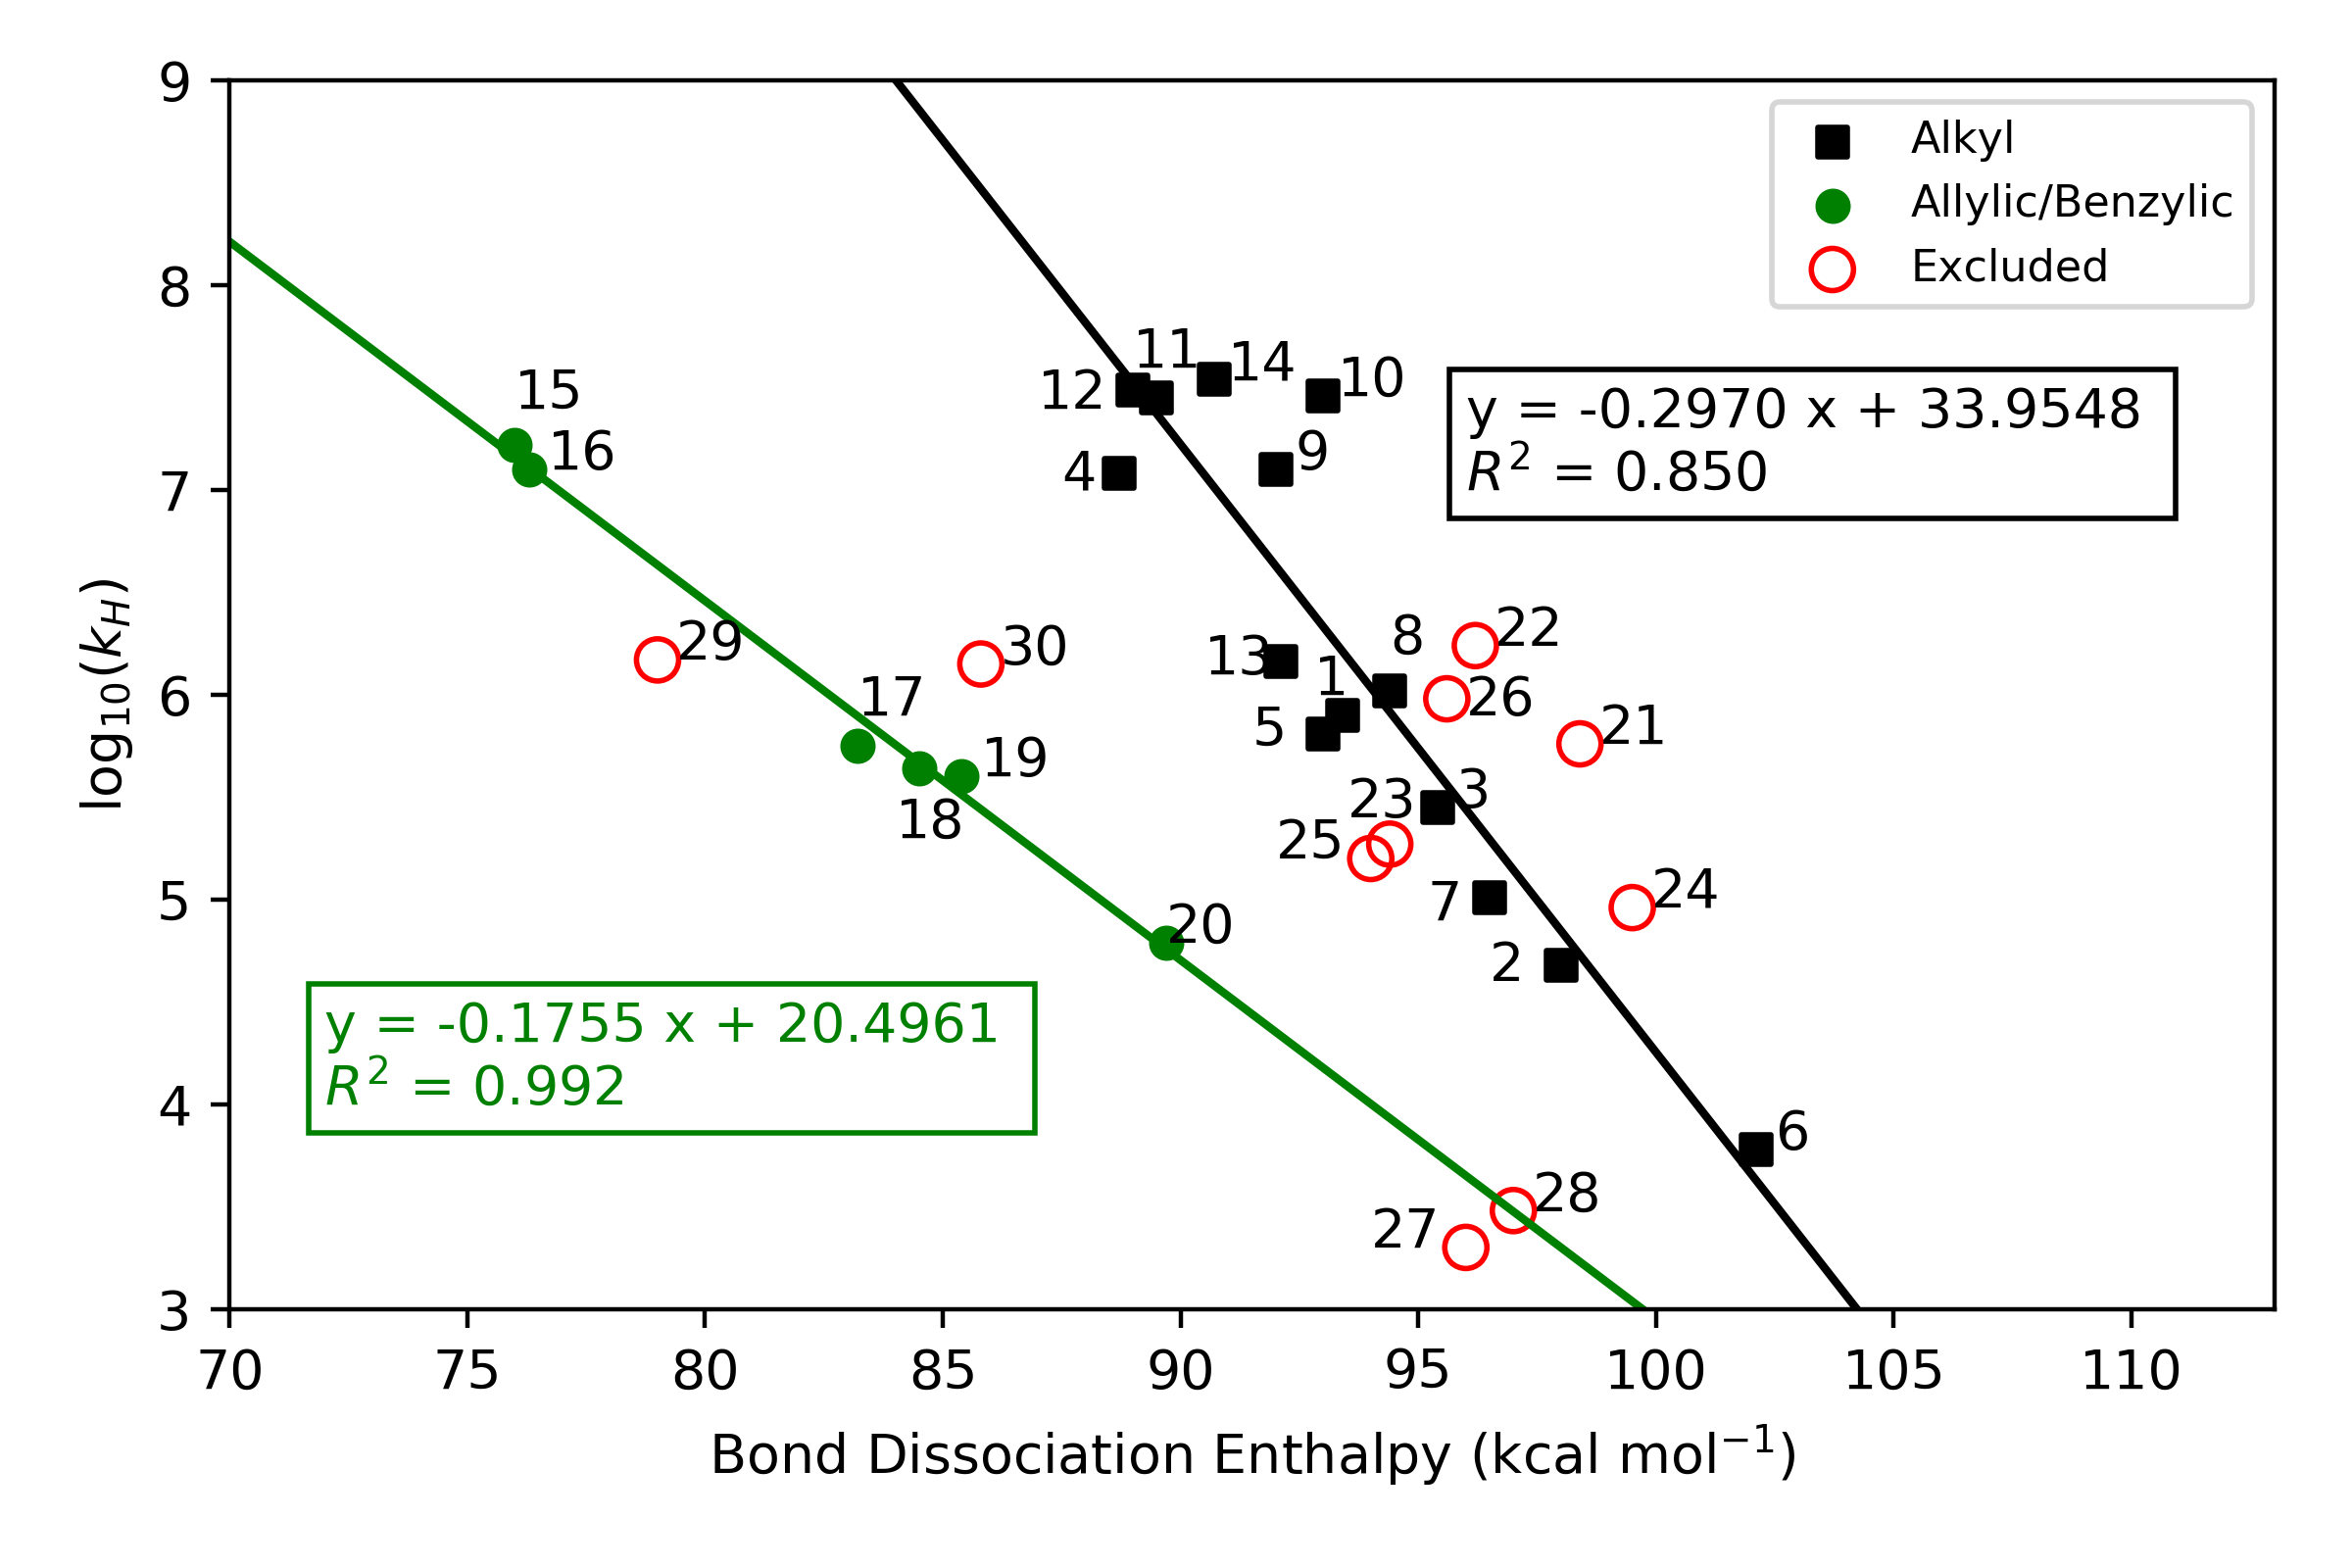
\includegraphics[width=\textwidth]{figures/bep-expt}
\begin{tabularx}{\textwidth}{| l X l X |}
  \hline
  1 & 1,4-diazobicyclo[2.2.2]octane & 2 & 2,2-dimethylbutane \\
  3 & 2,2-dimethylbutane & 4 & Benzaldehyde \\
  5 & Diethyl Ether & 6 & Dimethyl sulfoxide \\
  7 & Dioxane & 8 & Hexamethylphosphoramide \\
  9 & Morpholine & 10 & Piperazine \\
  11 & Piperidine & 12 & Pyrroldiine \\
  13 & Tetrahydrofuran & 14 & Triethylamine \\
  15 & 1,4-cyclohexadiene & 16 & 9,10-dihydroanthracene \\
  17 & Cumene & 18 & Diphenylmethane \\
  19 & Ethylbenzen & 20 & Toluene \\
  21 & Adamantane (2$^\circ$) & 22 & Adamantane (3$^\circ$) \\
  23 & Cycloheptane & 24 & Cyclohexane \\
  25 & Cyclooctane & 26 & Cyclopentane  \\
  27 & Acetone & 28 & Acetonitrile \\
  29 & Benzyl alcohol & 30 & Dibenzyl ether \\
  31 & Triphenylmethane & & \\
  \hline
\end{tabularx}
  \caption[Bell-Evans-Polanyi plot of experimental rate constants against literature BDEs.]{Bell-Evans-Polanyi plot of experimental rate constants (normalised for the number of equivalent hydrogen atoms) for HAT between \cumo~ and substrates against literature BDEs. BDEs for dimethyl sulfoxide and hexamethylphosphoramide are from Ref.~\protect\citenum{Salamone2012}, while all other BDEs are from Ref.~\protect\citenum{Luo2002}.}
\label{fig:bep-expt}
\end{figure}

There is a considerable amount of scatter in~\ref{fig:bep-expt}, which may be due to differences in experimental procedures. BDEs are measurable using a large number of different experimental techniques, and a great deal of data exists in the literature. Much of this data has conveniently been compiled in the \emph{de facto} reference for BDEs: the CRC Handbook of Bond Dissociation Enthalpies.\cite{Luo2002} However, caution must be taken with experimentally determined BDEs, as not all experimental methods give reliable data. For example, BDEs from the Bordwell\cite{Bordwell1988} thermochemical cycle are possibly unreliable.\cite{Salamone2012, Miller2016} This was demonstrated for the BDE of dimethyl sulfoxide (DMSO), for which the experimentally determined BDE is about 8 \kcalmol lower than the best computational estimate.\cite{Salamone2012} Therefore, quantum chemistry is a useful tool for studying BDEs, as it is facile to compute BDEs. An arbitrary \ch{X-H} bond dissociation enthalpy is given by:

\begin{equation}
  \Delta H(BDE) =  H(\ch{X^.}) + H(\ch{H^.}) - H(\ch{X-H})
\end{equation}

\noindent where $\Delta H(BDE)$ is the BDE, and the right-hand terms are the enthalpies of the radical product, the hydrogen atom, and the substrate, respectively. By computing the most accurate BDEs possible, we are able to discern if the BEP principle holds for \ch{C-H} bond hydrogen abstraction by \cumo.

DFT-based methods have been shown to give reliable relative BDEs, however, highly correlated wave function based methods are required to predict chemically accurate (sub-\kcalmol) BDEs.\cite{DiLabio1999, Chan2012, Wiberg2014} For this purpose, we shall use composite quantum chemical procedures. Unfortunately, due to the computational cost of some of these procedures, calculations are often limited to small molecules. Additionally, there is currently no literature which compares the ability of common composite methods to predict accurate BDEs. Therefore, another aim of the work is to determine which composite procedure can be used to calculate accurate BDEs for relatively large molecules.

\section{Methods}

Experimental rate constants were have either provided from unpublished results from our colleagues, the Bietti group in Rome, or come from literature sources.\cite{Bietti2010, Bietti2011, Pischel2001, Salamone2011, Salamone2012, Salamone2012a, Salamone2013, Salamone2015} All rate constants come from laser flash photolysis (LFP) experiments of \cumo~ with the substrates of interest. Acetonitrile solvent and ambient conditions (298 K and 1 atm) were used in all cases. For those results which have are unpublished, \cumo~ is generated by laser pulses at either 266 nm or 355 nm in solutions of excess dicumyl peroxide. Many of the literature results are also from the Bietti group, where the same procedure is used. Other results may have small variations in experimental details, however, all results are well time-resolved.

Observed rate constants ($k_{obs}$) are generally obtained from 4--8 averaged trials which are reproducible to within 5 \%. Transient absorption decay traces of \cumo~ monitored at 485 nm are used to determine $k_{obs}$. The observed rate constant is plotted against concentration of substrate to provide the bimolecular HAT rate constant ($k_H$) as the slope ($k_{obs} = k_0 + k_H[substrate]$). The \cumo~ radical decays unimolecularly through the $\beta$-scission of a methyl group, giving acetophenone and a methyl radical, as shown in~\ref{fig:cumo-decay}. The unimolecular decay rate constant\cite{Avila1993, Avila1995} for \cumo ($k_0$) in acetonitrile is on the order of 6.3 \E{5} s$^{-1}$ at 298 K.

\begin{scheme}[H]
  \centering
  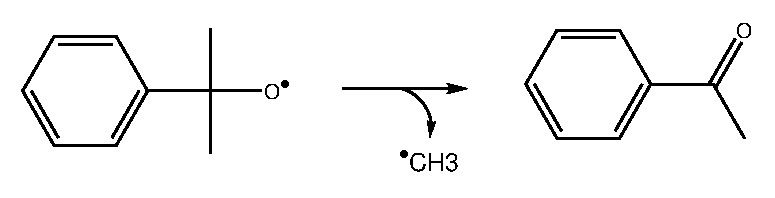
\includegraphics[width=0.75\textwidth]{figures/cumobeta.eps}
\caption{Unimolecular decay of the cumyloxyl radical.}
\label{fig:cumo-decay}
\end{scheme}

All quantum chemical calculations were performed using the Gaussian 09 software package.\cite{Frisch2009} Several composite quantum chemical method which are implemented in Gaussian 09 were used in this work: W1BD, CBS-QB3 and the restricted open-shell variant ROCBS-QB3, CBS-APNO, and G4 and the MP2 variant G4(MP2). An approach using ROCCSD(T) with locally-dense basis sets\cite{DiLabio1999LDBS, Wright2001} (LDBS) was also utilised in order to approximate W1BD results. Each of these methods is briefly described below.


\subsection{Quantum chemical composite procedures}

\noindent \textbf{W1BD}

The highest accuracy method used is W1BD, which employs seven different calculations to obtain highly correlated electronic energies, as well as thermochemically corrected quantities. This method is very computationally expensive, and thus cannot be applied to the larger species of interest in this work. Geometries and thermochemical corrections come from DFT-based B3LYP calculations with nearly complete cc-pVTZ+d basis sets. A frequency scaling factor of 0.985 is used to obtain thermochemical corrections. The electronic energy comes from several additive corrections involving the Brueckner Doubles\cite{Barnes2009} (BD) variation of coupled cluster and large basis sets extrapolated to the complete basis set limit. Corrections for core-electron correlation and relativistic contributions are computed using an uncontracted variant of the cc-pVTZ+2df basis sets, known as MTsmall.\cite{Martin1999}
\\

\noindent \textbf{LDBS approach}

Locally-dense basis sets have been used in the past to calculated BDEs for relatively large molecules.\cite{DiLabio1998, DiLabio1999LDBS, Wright2001} The principle  behind LDBS is to use large basis sets to treat the atomic centres which are directly involved in the chemistry taking place, and use to progressively smaller basis sets for ``remote'' portions of the molecule, thus taking advantage of error cancellation. We chose a method which best approximate W1BD results for a small subset of molecules. The scheme utilised herein involves geometry optimisation and scaled frequencies calculations from DFT-based B3LYP/cc-pVTZ+d, as used in the W1BD procedure. Single-point energy calculations are then performed using ROCCSD(T) and an LDBS partitioning scheme we denote as pc-3/3/2/1, demonstrated in~\ref{fig:ldbs}, which uses the polarisation consistent basis sets.\cite{Jensen2001}

\begin{scheme}[H]
\centering
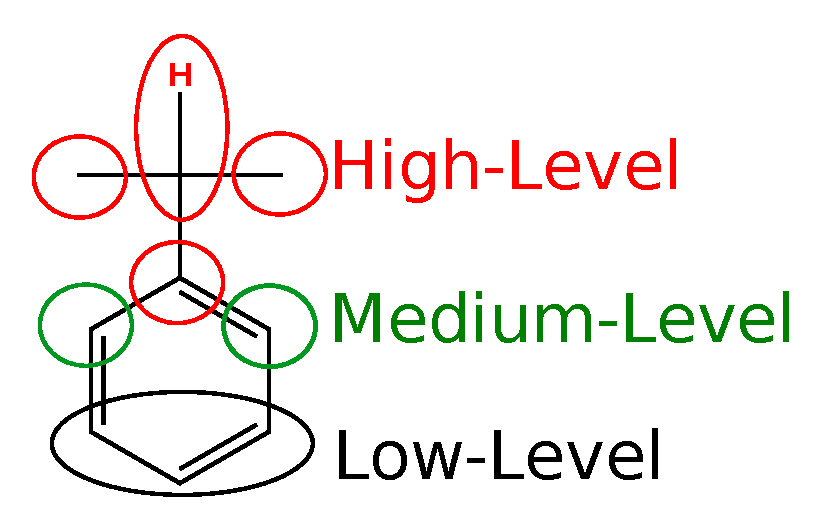
\includegraphics[width=\textwidth]{figures/ldbs.eps}
\caption[Locally-dense basis set partitioning used in the calculation of BDEs.]{Locally-dense basis set partitioning used in the calculation of BDEs. The scheme is referred to as pc-3/3/2/1, where for the shown cumene molecule, the centre of \ch{C-H} cleavage and the immediately adjacent groups are treated with high-level pc-3 basis sets. The next groups are treated with medium level pc-2 basis sets, and all other atoms/groups are treated with low-level pc-1 basis sets.}
\label{fig:ldbs}
\end{scheme}

\noindent \textbf{CBS methods}

The Complete Basis Set (CBS) methods of Petersson and coworkers\cite{Montgomery1999, Montgomery2000, Ochterski1996, Wood2006} are widely used because of the relatively low computational cost (compared to other composite procedures), and well established accuracy.\cite{Somers2015, Simmie2015} CBS-QB3\cite{Montgomery1999, Montgomery2000} utilises DFT-based B3LYP optimisation and scaled frequencies (factor = 0.990) with modified triple-zeta Pople style basis sets. Electronic energies are obtained by extrapolation of medium basis set CCSD(T) and MP4SDQ. Small empirical corrections for are added to achieve more accurate results compared to the parametrisation sets.\cite{Petersson2001} ROCBS-QB3 is a similar procedure to CBS-QB3, except spin-restricted wave functions are used in place of unrestricted wave functions. This is done to eliminate spin contamination, and the use of an restricted open-shell definition has been shown to produce more accurate BDEs.\cite{DiLabio1999} The (RO)CBS-QB3 methods have been implemented for the first, second, and third periods of elements.

Atomic pair natural orbital (APNO) expansions are a method used for averaging over multiple Slater determinants. The use of APNOs allows for small basis set extrapolation of higher order correlation energies to converge more rapidly to the complete basis set limit. This approach is used in the CBS-APNO method.\cite{Ochterski1996} Geometries and scaled frequencies (factor = 0.989) are obtained at the QCISD/6-311G(d,p) level of theory. Similar to CBS-QB3, the extrapolation of moderate basis set MP4SDQ and QCISD(T) results gives the electronic energy. An empirical correction is also used in CBS-APNO. Although CBS-APNO is more accurate, the expansion of APNOs makes CBS-APNO more computationally demanding than CBS-QB3. As a result, CBS-APNO has only been implemented for first and second row periods, and is thus less commonly used in the literature.
\\

\noindent \textbf{G$n$ methods}

The Gaussian$-n$ (G$n$) series of methods originates from the Pople group,\cite{Pople1989} where G4 is the fourth generation. G4 utilises moderately large basis sets and extrapolation techniques with CCSD(T) calculations to obtained highly correlated electronic energies. G4(MP2) uses MP2 in place is CCSD(T) and is thus less computationally expensive, but also gives a less complete description of electron correlation. Both methods use the B3LYP/6-31(2df,p) level of theory for optimisation and frequency calculations with a frequency scaling factor of 0.9854. G4 results have been described as generally on par with CBS-QB3 results,\cite{Somers2015, Simmie2015} but calculations are more computationally expensive.

\subsection{Transition state calculations}

Calculations were performed to identify the lowest energy TS complex of several reactions between \cumo~ and organic substrates. In all cases cisoid and transoid conformations were explored. All optimisation calculations were performed at the B3LYP-D3(BJ)/6-31+G$^*$ level of theory, followed by single-point energy calculations at the LC-$\omega$PBE-D3(BJ)/6-311+G$^{**}$ level of theory. The latter DFT-based method was selected to minimise delocalisation error in the TS complex.\cite{OterodelaRoza2014} Transition states were visualised using the Chemcraft program\cite{ccraft} to confirm a single imaginary frequency connecting reactants to products. In some cases, a small secondary imaginary frequency was observed, indicating a TS complex which is not fully optimised. Necessary steps were taken to re-optimise the structures and eliminate the small imaginary frequencies, however, this was not always successful. Nonetheless, I am confident the structures reported herein sufficiently represent the true TS complex geometries and relative energies. Results from structures which are not fully optimised are indicated appropriately as such.

\section{Comparison of composite method for the prediction of BDEs}

In order to determine the best method for BEP principle analysis, and to investigate which is the most efficient yet accurate composite method, the BDEs of 50 species have been calculated. This set of species contains a wide variety of chemical functionalities with BDEs ranging from 75--113 \kcalmol, thus this set may be described as a comprehensive test of these methods for C-H BDEs. Given that W1BD is the most accurate method used, these results have been used for comparison to other composite method. However, BDEs for only 33 out of the 49 species studied were able to be calculated using W1BD due to computational cost restrictions: hard disk capacity was insufficient for large systems. Therefore, literature BDEs from \citet{Luo2002} for the 49 species which have literature values in the set are also used for comparison. The literature and calculated BDEs are listed in~\ref{tab:bde-calc}.

\begin{landscape}
%\singlespacing
\begin{longtable}{m{3.1cm} | c c c c c c c c}
\caption[Bond dissociation enthalpies of the species used to investigate the accuracy of composite methods.]{Bond dissociation enthalpies of the species used to investigate the accuracy of composite methods. All values are in \kcalmol. Statistics are listed at the bottom of the table.} \label{tab:bde-calc} \\
Molecule                         &  Lit.\cite{Luo2002}      &   W1BD   &     LDBS &     CBS-QB3 &   ROCBS-QB3 &   CBS-APNO &    G4   &    G4(MP2)\\
\hline
\endfirsthead
Molecule                         &  Lit.\cite{Luo2002}      &   W1BD   &     LDBS &     CBS-QB3 &   ROCBS-QB3 &   CBS-APNO &    G4   &    G4(MP2)\\
\hline
\endhead
1,3-pentadiene                   &  83.0     &   82.9   &   82.2   &    80.9     &    81.7    &   81.8   &  81.6   &    82.1   \\
1,4-diazabicyclo[2.2.2]-octane   &  93.4     &          &   98.9   &    98.9     &    98.8    &   98.5   &  96.7   &    95.6   \\
1,4-pentadiene                   &  76.6     &   76.2   &   76.0   &    74.2     &    75.0    &   75.2   &  75.1   &    75.7   \\
2,2-dimethylbutane               &  98.0     &   99.3   &   99.1   &    99.4     &    99.3    &   99.7   &  97.5   &    96.7   \\
2,3-dimethylbutane               &  95.4     &   97.8   &   97.7   &    97.9     &    97.8    &   98.0   &  96.2   &    95.5   \\
2-methylbutane                   &  95.8     &   97.3   &   97.2   &    97.3     &    97.1    &   97.3   &  95.9   &    95.5   \\
Acetaldehyde                     &  94.3     &   95.9   &   95.3   &    95.3     &    95.7    &   95.5   &  94.9   &    94.8   \\
Acetone                          &  96.0     &   96.9   &   96.4   &    96.2     &    96.7    &   97.1   &  95.4   &    95.0   \\
Acetonitrile                     &  97.0     &   96.9   &   96.6   &    96.2     &    96.6    &   96.5   &  96.3   &    96.3   \\
Adamantane (2$^\circ$)           &  98.4     &          &  100.9   &   100.5     &   100.4    &  100.9   &  97.8   &    96.3   \\
Adamantane (3$^\circ$)           &  96.2     &          &  100.3   &    99.9     &    99.9    &  100.3   &         &    95.7   \\
Benzaldehyde                     &  88.7     &          &   90.9   &    91.5     &    91.4    &   91.0   &  89.3   &    88.2   \\
Benzene                          & 112.9     &  113.1   &  112.7   &   115.4     &   113.0    &          &         &   113.0   \\
Benzyl Alcohol                   &  79.0     &          &   84.4   &    84.3     &    83.2    &   83.9   &  83.4   &    83.6   \\
Cumene                           &  83.2     &          &   87.9   &    87.9     &    86.9    &          &  86.9   &    86.7   \\
Cycloheptane                     &  94.0     &          &   96.0   &    96.0     &    95.8    &   96.1   &  93.9   &    92.9   \\
Cyclohexadiene                   &  76.0     &   76.3   &   76.2   &    74.3     &    75.0    &          &  75.2   &    75.5   \\
Cyclohexane                      &  99.5     &   99.2   &   99.1   &    99.4     &    99.3    &   99.6   &  97.5   &    96.8   \\
Cyclooctane                      &  94.4     &          &   92.6   &    92.6     &    92.4    &   92.8   &  90.2   &    89.1   \\
Cyclopentane                     &  95.6     &   96.3   &   96.1   &    96.5     &    96.3    &   96.6   &  95.6   &    95.0   \\
Cyclopropane                     & 106.3     &  109.0   &  108.5   &   109.3     &   109.2    &  109.5   & 108.2   &   108.0   \\
Dibenzyl ether                   &  85.8     &          &   83.6   &    84.3     &    82.7    &          &         &    79.6   \\
Diethyl ether                    &  93.0     &   95.3   &   95.1   &    95.6     &    95.5    &   95.4   &  93.8   &    93.1   \\
Dihydroanthracene                &  76.3     &          &   80.4   &    80.9     &    78.1    &          &         &    79.9   \\
Dimethylamine                    &  94.2     &   92.6   &   92.4   &    92.9     &    92.8    &   92.7   &  92.0   &    91.9   \\
Dimethylsulfoxide                &  94.0     &  102.0   &  101.7   &   102.3     &   102.3    &          & 100.9   &   100.6   \\
Dioxane                          &  96.5     &   97.3   &   97.3   &    97.7     &    97.6    &   97.4   &  95.7   &    94.9   \\
Diphenylmethane                  &  84.5     &          &   84.1   &    85.3     &    82.8    &          &         &    84.5   \\
Ethane                           & 100.5     &  101.3   &   99.3   &   101.7     &   101.5    &  101.8   & 100.7   &   100.7   \\
Ethylbenzene                     &  85.4     &          &   88.3   &    88.6     &    87.6    &   89.3   &  87.6   &    87.7   \\
Ethylene                         & 110.9     &  110.8   &  110.3   &   110.6     &   110.9    &  111.1   & 109.9   &   110.2   \\
Fluorene                         &  82.0     &          &   82.4   &    83.6     &    81.9    &          &         &    81.2   \\
Formaldehyde                     &  88.0     &   88.6   &   88.0   &    89.1     &    88.9    &   88.2   &  88.2   &    87.9   \\
Hexamethyl-phosphoramide         &           &          &   93.8   &    94.1     &    93.9    &          &         &    88.5   \\
Indene                           &  83.0     &          &   80.6   &    80.4     &    80.1    &   81.2   &  79.0   &    78.3   \\
Methane                          & 105.0     &  105.0   &  104.4   &   105.4     &   105.2    &  105.4   & 104.5   &   104.6   \\
Methanol                         &  96.1     &   96.4   &   96.0   &    96.9     &    96.8    &   96.6   &  96.0   &    95.8   \\
Methylamine                      &  93.9     &   93.1   &   92.8   &    93.4     &    93.3    &   93.3   &  92.7   &    92.8   \\
Morpholine                       &  92.0     &          &   93.4   &    93.4     &    93.3    &   93.3   &  91.8   &    91.1   \\
N,N-dimethylacetamide (acetyl)   &  91.4     &   99.6   &   99.4   &    99.5     &    99.5    &  100.1   &  97.6   &    96.8   \\
Piperazine                       &  93.0     &   93.4   &   93.5   &    93.6     &    93.5    &   93.4   &  91.9   &    91.2   \\
Piperidine                       &  89.5     &   92.1   &   92.2   &    92.3     &    92.2    &   92.1   &  90.7   &    90.0   \\
Propane                          & 100.9     &  101.6   &  101.3   &   102.0     &   101.8    &  102.1   & 100.7   &   100.4   \\
Pyrrolidine                      &  89.0     &   90.8   &   90.6   &    90.8     &    90.7    &   90.7   &  89.5   &    89.0   \\
Tetrahydro-2H-pyran              &  96.0     &   96.3   &   96.2   &    96.6     &    96.5    &   96.3   &  94.7   &    93.9   \\
Tetrahydrofuran                  &  92.1     &   93.7   &   93.3   &    93.9     &    93.8    &   93.6   &  92.2   &    91.6   \\
Toluene                          &  89.7     &   90.5   &   90.1   &    90.6     &    89.7    &   91.9   &  89.8   &    90.2   \\
Trichloromethane                 &  93.8     &   93.5   &   93.4   &    93.8     &    93.7    &          &  92.4   &    92.0   \\
Triethylamine                    &  90.7     &          &   91.4   &    91.3     &    91.2    &   91.4   &  89.4   &    88.4   \\
Trifluormethane                  & 106.4     &  107.2   &  106.6   &   107.4     &   107.4    &  106.8   & 105.8   &   105.0   \\
\hline
\textbf{Statistics}             & Lit.       &  W1BD    &    LDBS  &    CBS-QB3  &  ROCBS-QB3  &  CBS-APNO &    G4  &    G4(MP2)\\
\hline
Number of BDEs ($N$) &    49     &     33   &     50   &      50     &      50     &     40    &    43   &     50   \\
MAE (Lit.)                       &           &   0.82   &   1.60   &    1.88     &    1.64     &   1.35    &  1.21   &   1.57   \\
Max. Error                             &           &   1.59   &   2.41   &    2.63     &    3.15     &   1.85    &  4.19   &   6.23   \\
Min. Error                           &           &  -8.22   &  -8.04   &   -8.26     &   -8.25     &  -8.74    & -6.86   &  -6.58   \\
MAE (W1BD)                       &           &          &   0.22   &    0.32     &    0.18     &   0.20    &  0.70   &   0.88   \\
Max. Error                            &           &          &   2.00   &    2.01     &    1.26     &   1.08    &  2.05   &   2.84   \\
Min. Error                            &           &          &  -0.09   &   -2.37     &   -0.35     &  -1.39    &  0.37   &   0.02   \\
\end{longtable}

\end{landscape}

Mean absolute error (MAE) is used to assess the quality of computational methods, where errors are calculated with respect to benchmark values for a given data set.\cite{Savin2014} The MAE is calculated as

\begin{equation}
  \mathrm{MAE} = \frac{1}{N} \sum | E_{ref} - E_{calc}|
\end{equation}

\noindent where, for a set of $N$ reference values, the MAE is the average of the mean differences of the reference energy ($E_{ref}$) and the calculated value ($E_{calc}$). The MAE with respect to W1BD and literature shall be reported herein as ``MAE$_{\mathrm{W1BD}}$ (MAE$_{\mathrm{Lit.}}$)''. An additional semi-quantitative metric which I used to evaluate the accuracy of composite procedures to reproduce experimental results, is a bar chart which summarises the number of deviations from literature within given error ranges. This bar chart is reported in~\ref{fig:maebarchart}. Note that calculations for some species with some methods failed to converge, thus number of BDEs out of 49 are also shown in~\ref{fig:maebarchart} Also, an alternative method which I shall utilise for reporting these data is through the use of one-to-one plots, in which BDEs from two methods are directly compared. An ideal plot should have a slope = 1 and y-intercept = 0.

\begin{figure}[!htbp]
  \centering
  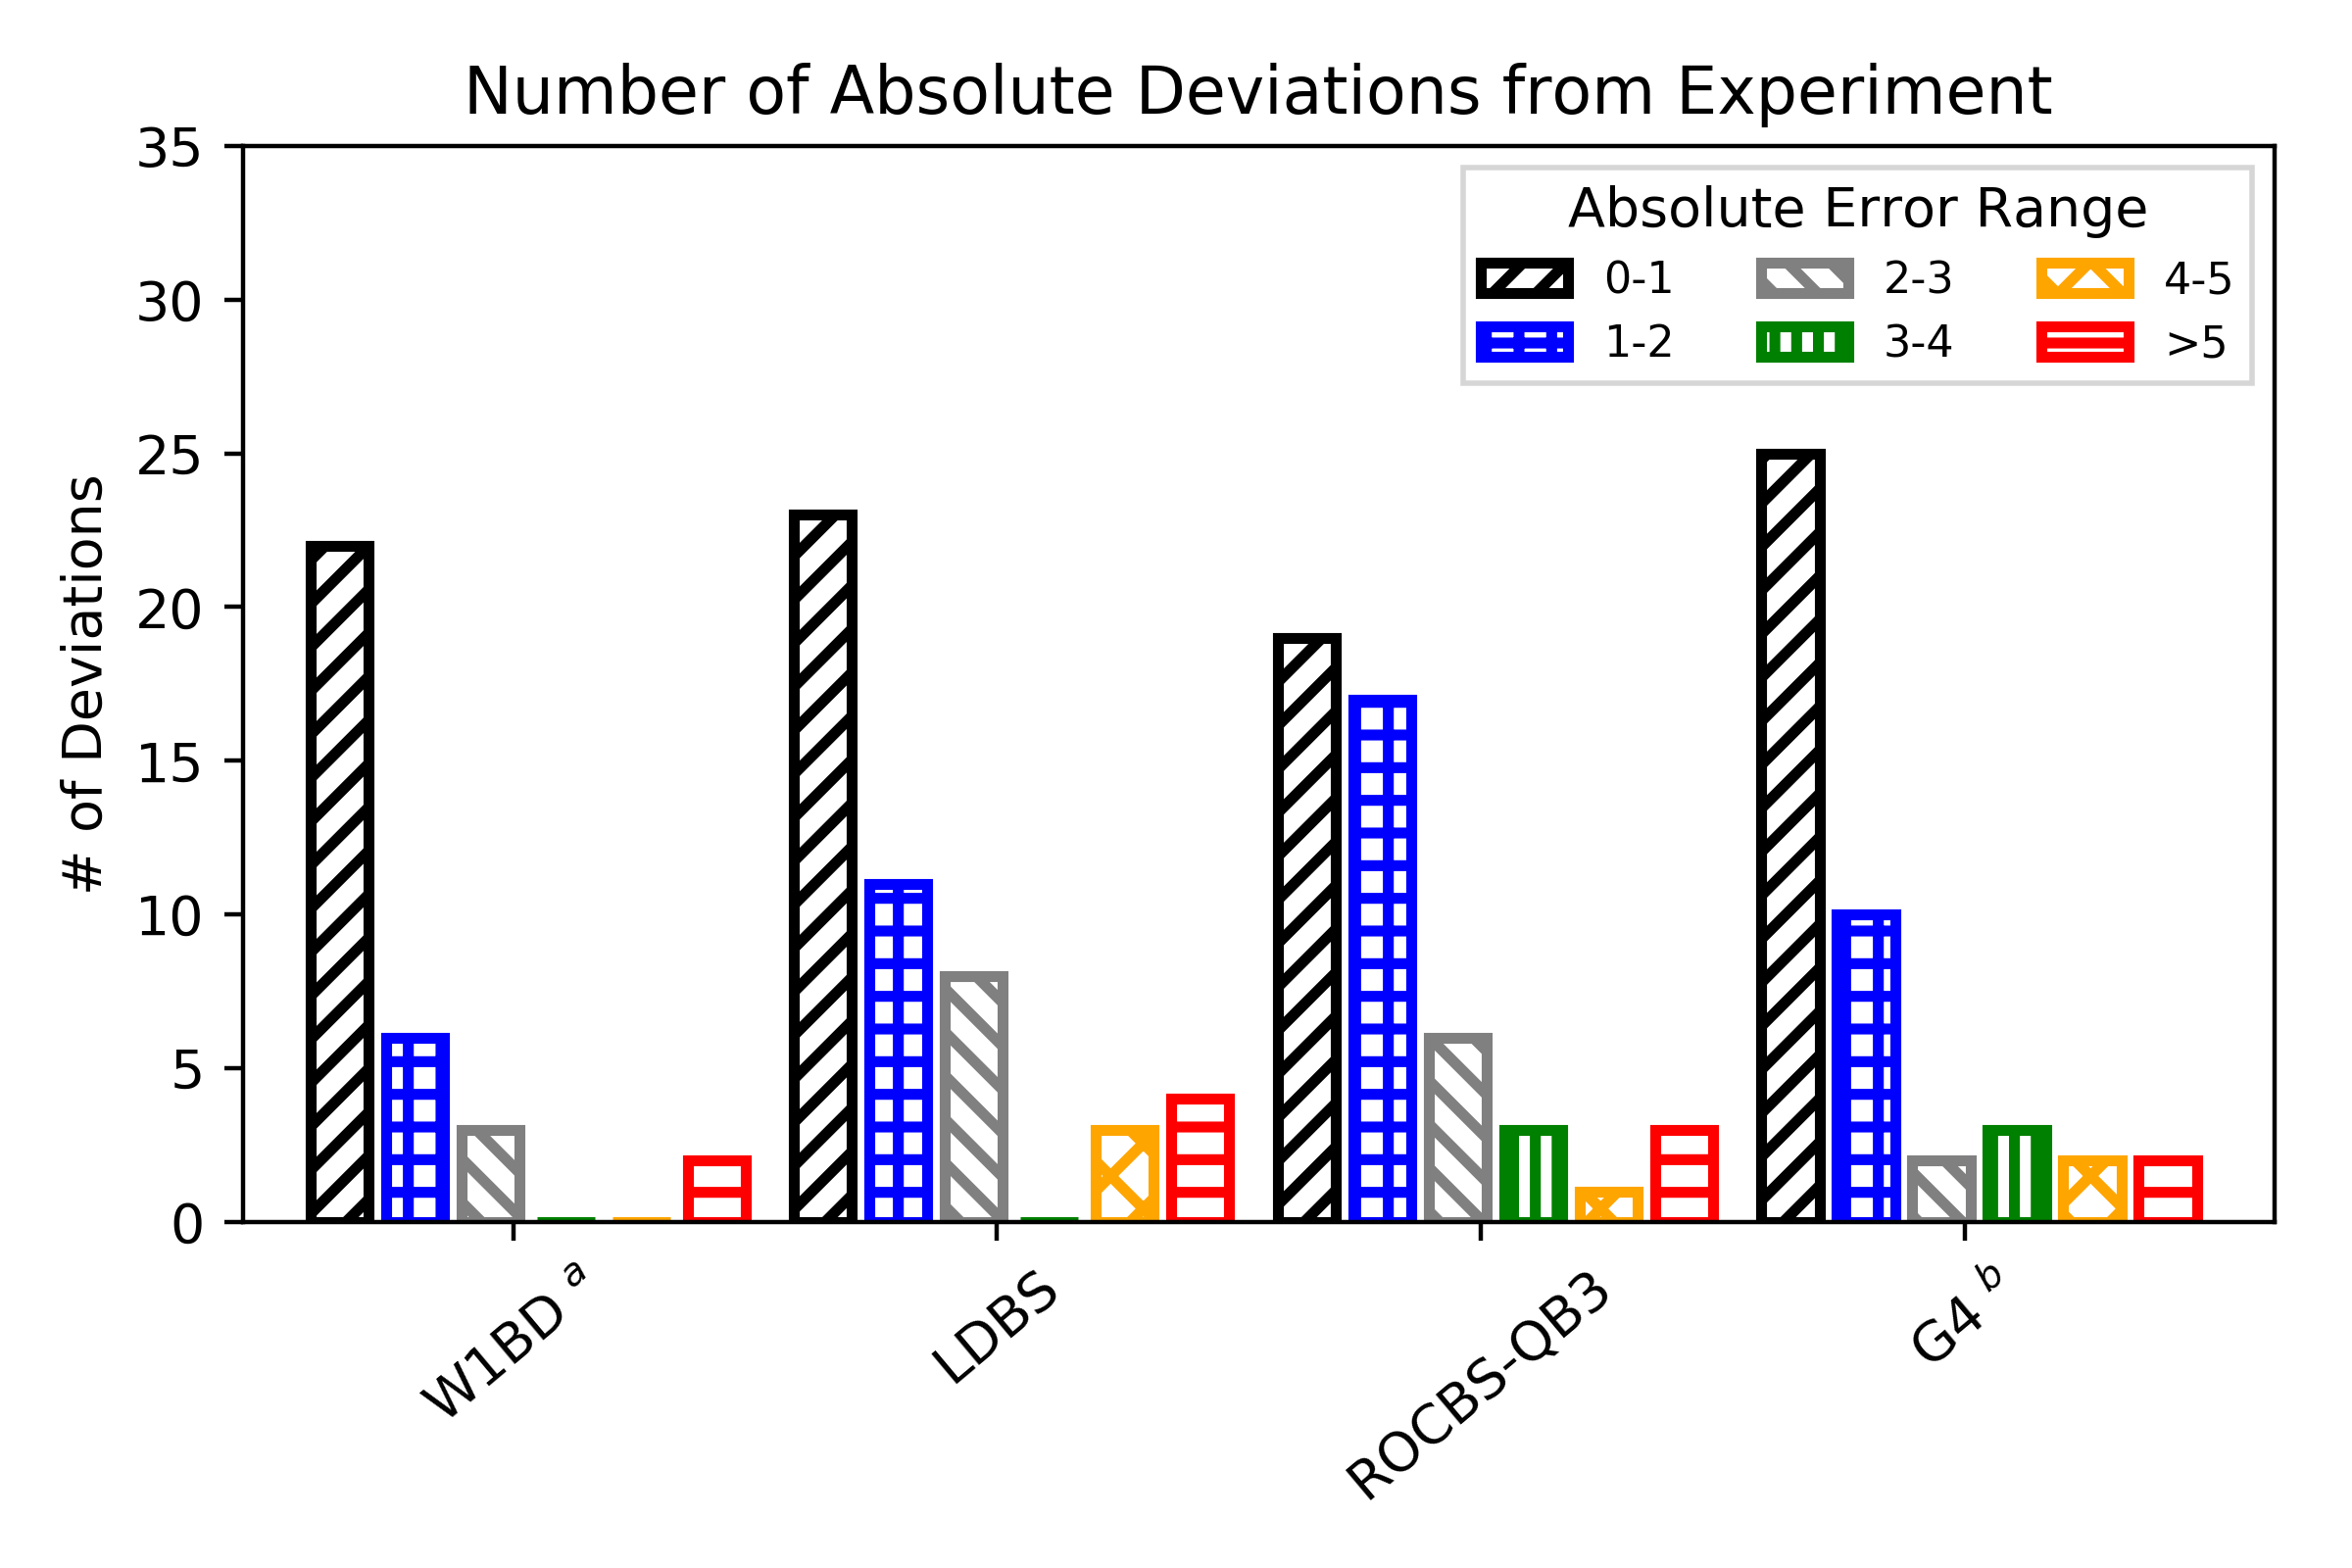
\includegraphics[width=\textwidth]{figures/bde-barchart}
  \caption[Summary of deviations of BDEs from literature for composite quantum chemical methods.]{Summary of deviations of BDEs from literature or composite quantum chemical methods. Errors are units of \kcalmol and are relative to Reference~\protect\citenum{Luo2002}. Numbers out of 49 represent the total number of data points which were computed for the given method.}
  \label{fig:maebarchart}
\end{figure}

Comparing W1BD results to literature, the MAE is 0.82 \kcalmol, and the majority of the data matching to within 1--2 \kcalmol of literature. Thus, W1BD is largely consistent with the literature values. Additionally, the one-to-one plots comparing W1BD to literature in~\ref{fig:1-1-W1BD}, show reasonable agreement with slope of 0.98 and a y-intercept of 2.35. There are, however, two large outliers: DMSO\footnotemark~ and \emph{N,N}-dimethylacetamide, where experiment underestimates the BDEs by -8.0 and -8.2 \kcalmol, respectively. These large outliers are consistent amongst all composite method, suggesting the literature BDEs for DMSO and \emph{N,N}-dimethylacetamide are incorrect.

\footnotetext{The experimental BDE for dimethyl sulfoxide was previously identified as inaccurate by Salamone et al.\protect\cite{Salamone2012}}

\begin{figure}[H]
  \centering
  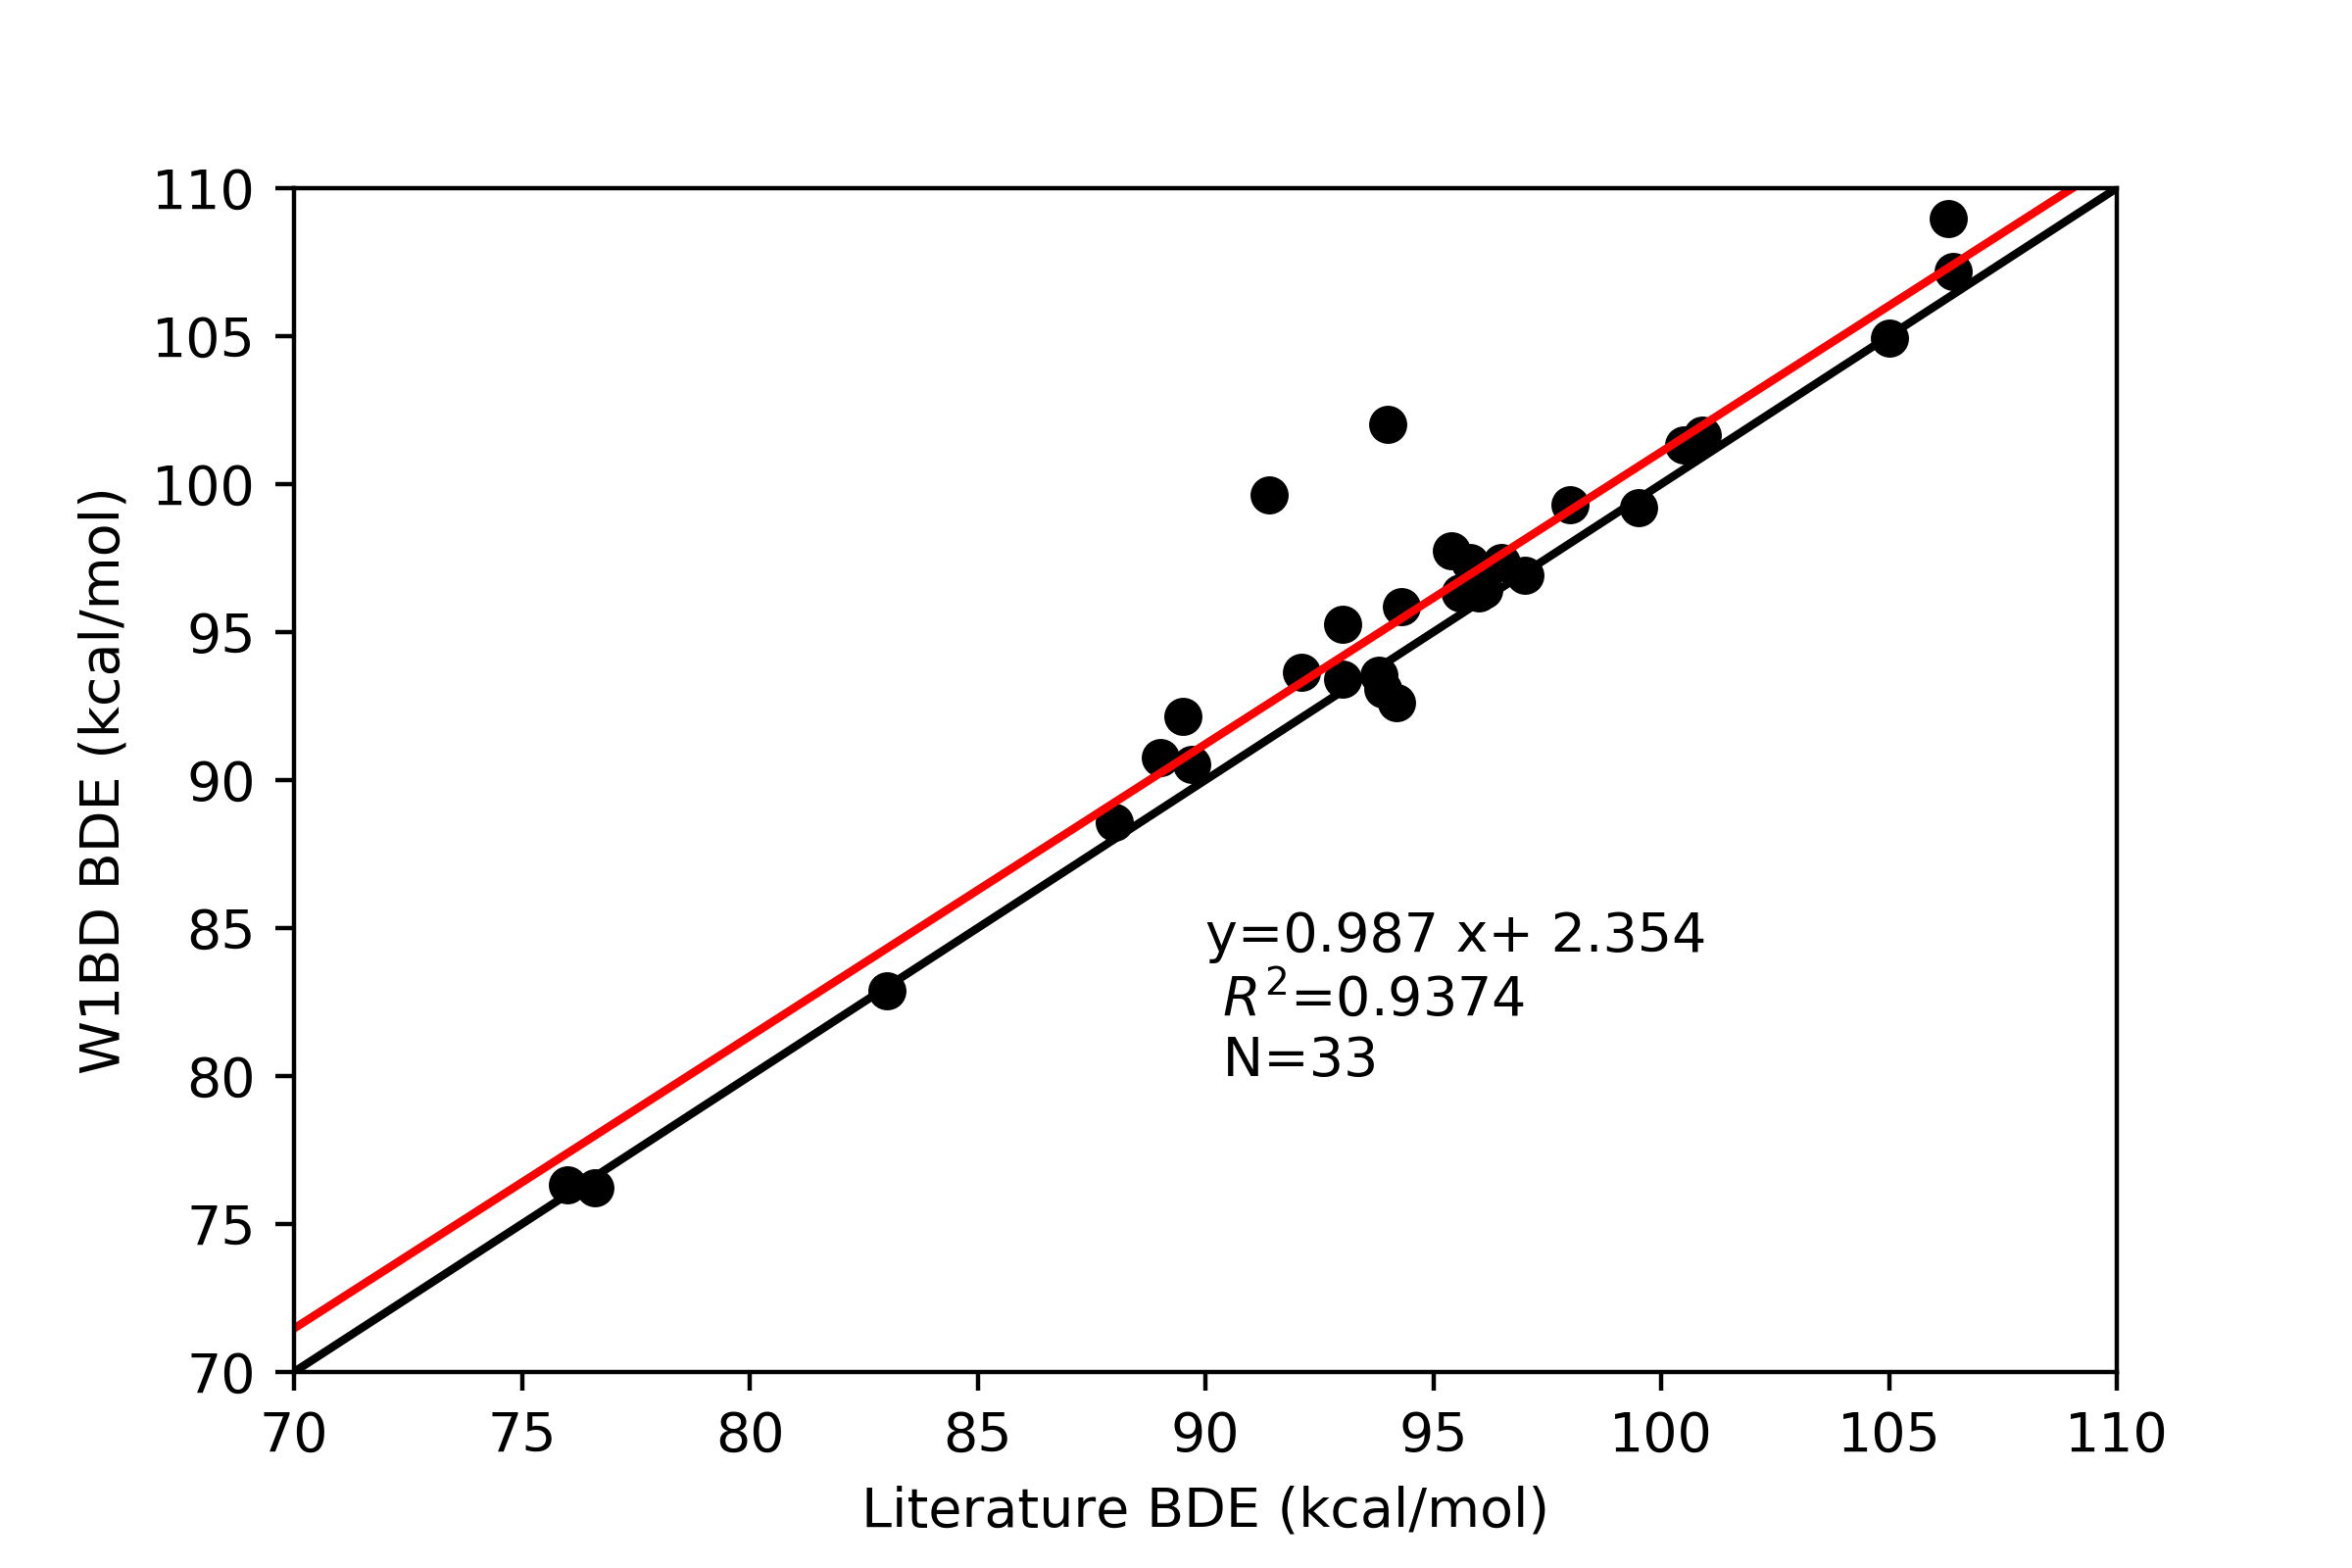
\includegraphics[width=\textwidth]{figures/lit-w1bd}
  \caption[One-to-one plot of BDEs from literature and as calculated by the W1BD composite method.]{One-to-one plot of BDEs from literature\protect\cite{Luo2002} and as calculated by the W1BD composite method. The red line represents the least squares line of best fit, while black line represents a perfect one-to-one correlation.}
  \label{fig:1-1-W1BD}
\end{figure}

The method which gives the best combined agreement with W1BD and literature is ROCBS-QB3 with an MAE = 0.18 (1.64) \kcalmol. It is also apparent from the one-to-one plots in~\ref{fig:1-1-ROCBSQB3}, that ROCBS-QB3 matches well with literature and experiment. In comparison, CBS-QB3 has an MAE = 0.32 (1.88) \kcalmol, while CBS-APNO has an MAE = 0.20 (1.40) \kcalmol. The LDBS approach also performs well with an MAE = 0.22 (1.60) \kcalmol. The G4 method deviates from the W1BD reference by about 0.5 \kcalmol more, however, it appears to give reasonable agreement with experimental results (MAE = 0.70 (1.21) mol). The use of the MP2 variant of G4 gives somewhat questionable results, with an MAE of 0.88 (1.60) \kcalmol, as well as a large outlier of 6.2 kcal/mol that is not present in the other data from composite methods. One-to-one plots of all other methods are presented in Appendix~\ref{ap:bde}.

\begin{figure}[H]
  \hspace*{-1.5cm}
  \begin{minipage}{8cm}
    \centering
    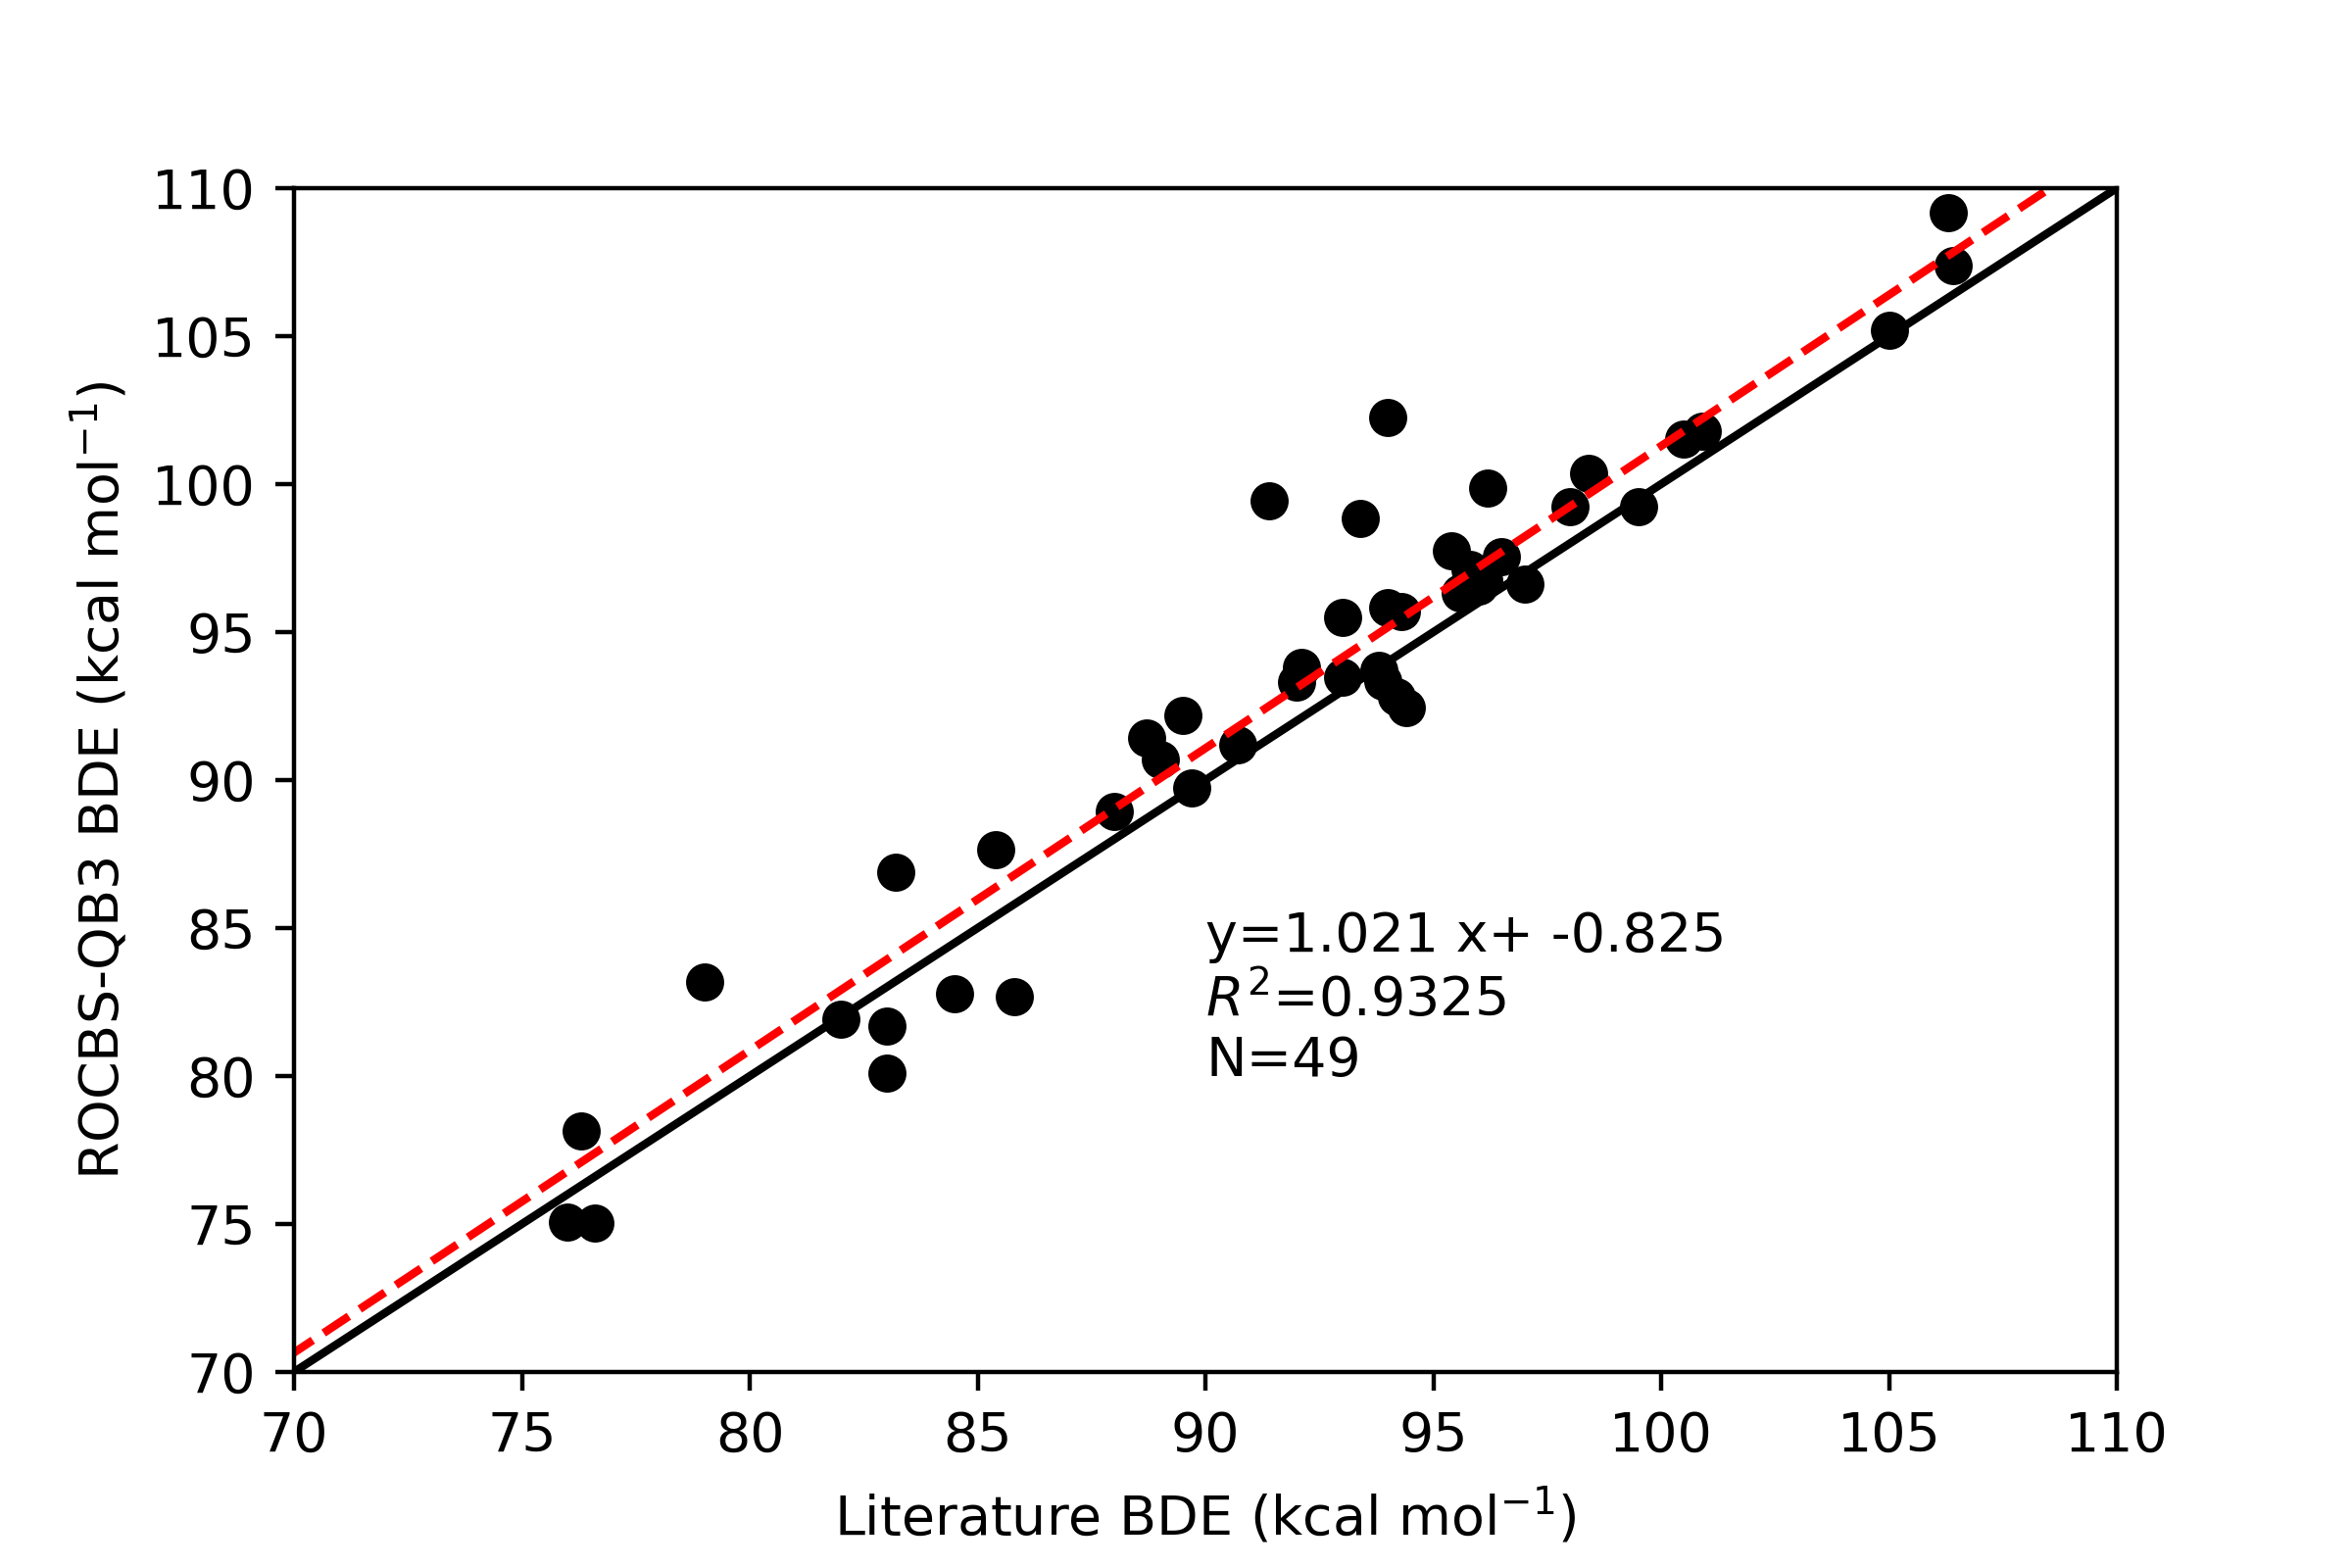
\includegraphics[width=\textwidth]{figures/lit-rocbsqb3}
  \end{minipage}%
  \begin{minipage}{8cm}
    \centering
    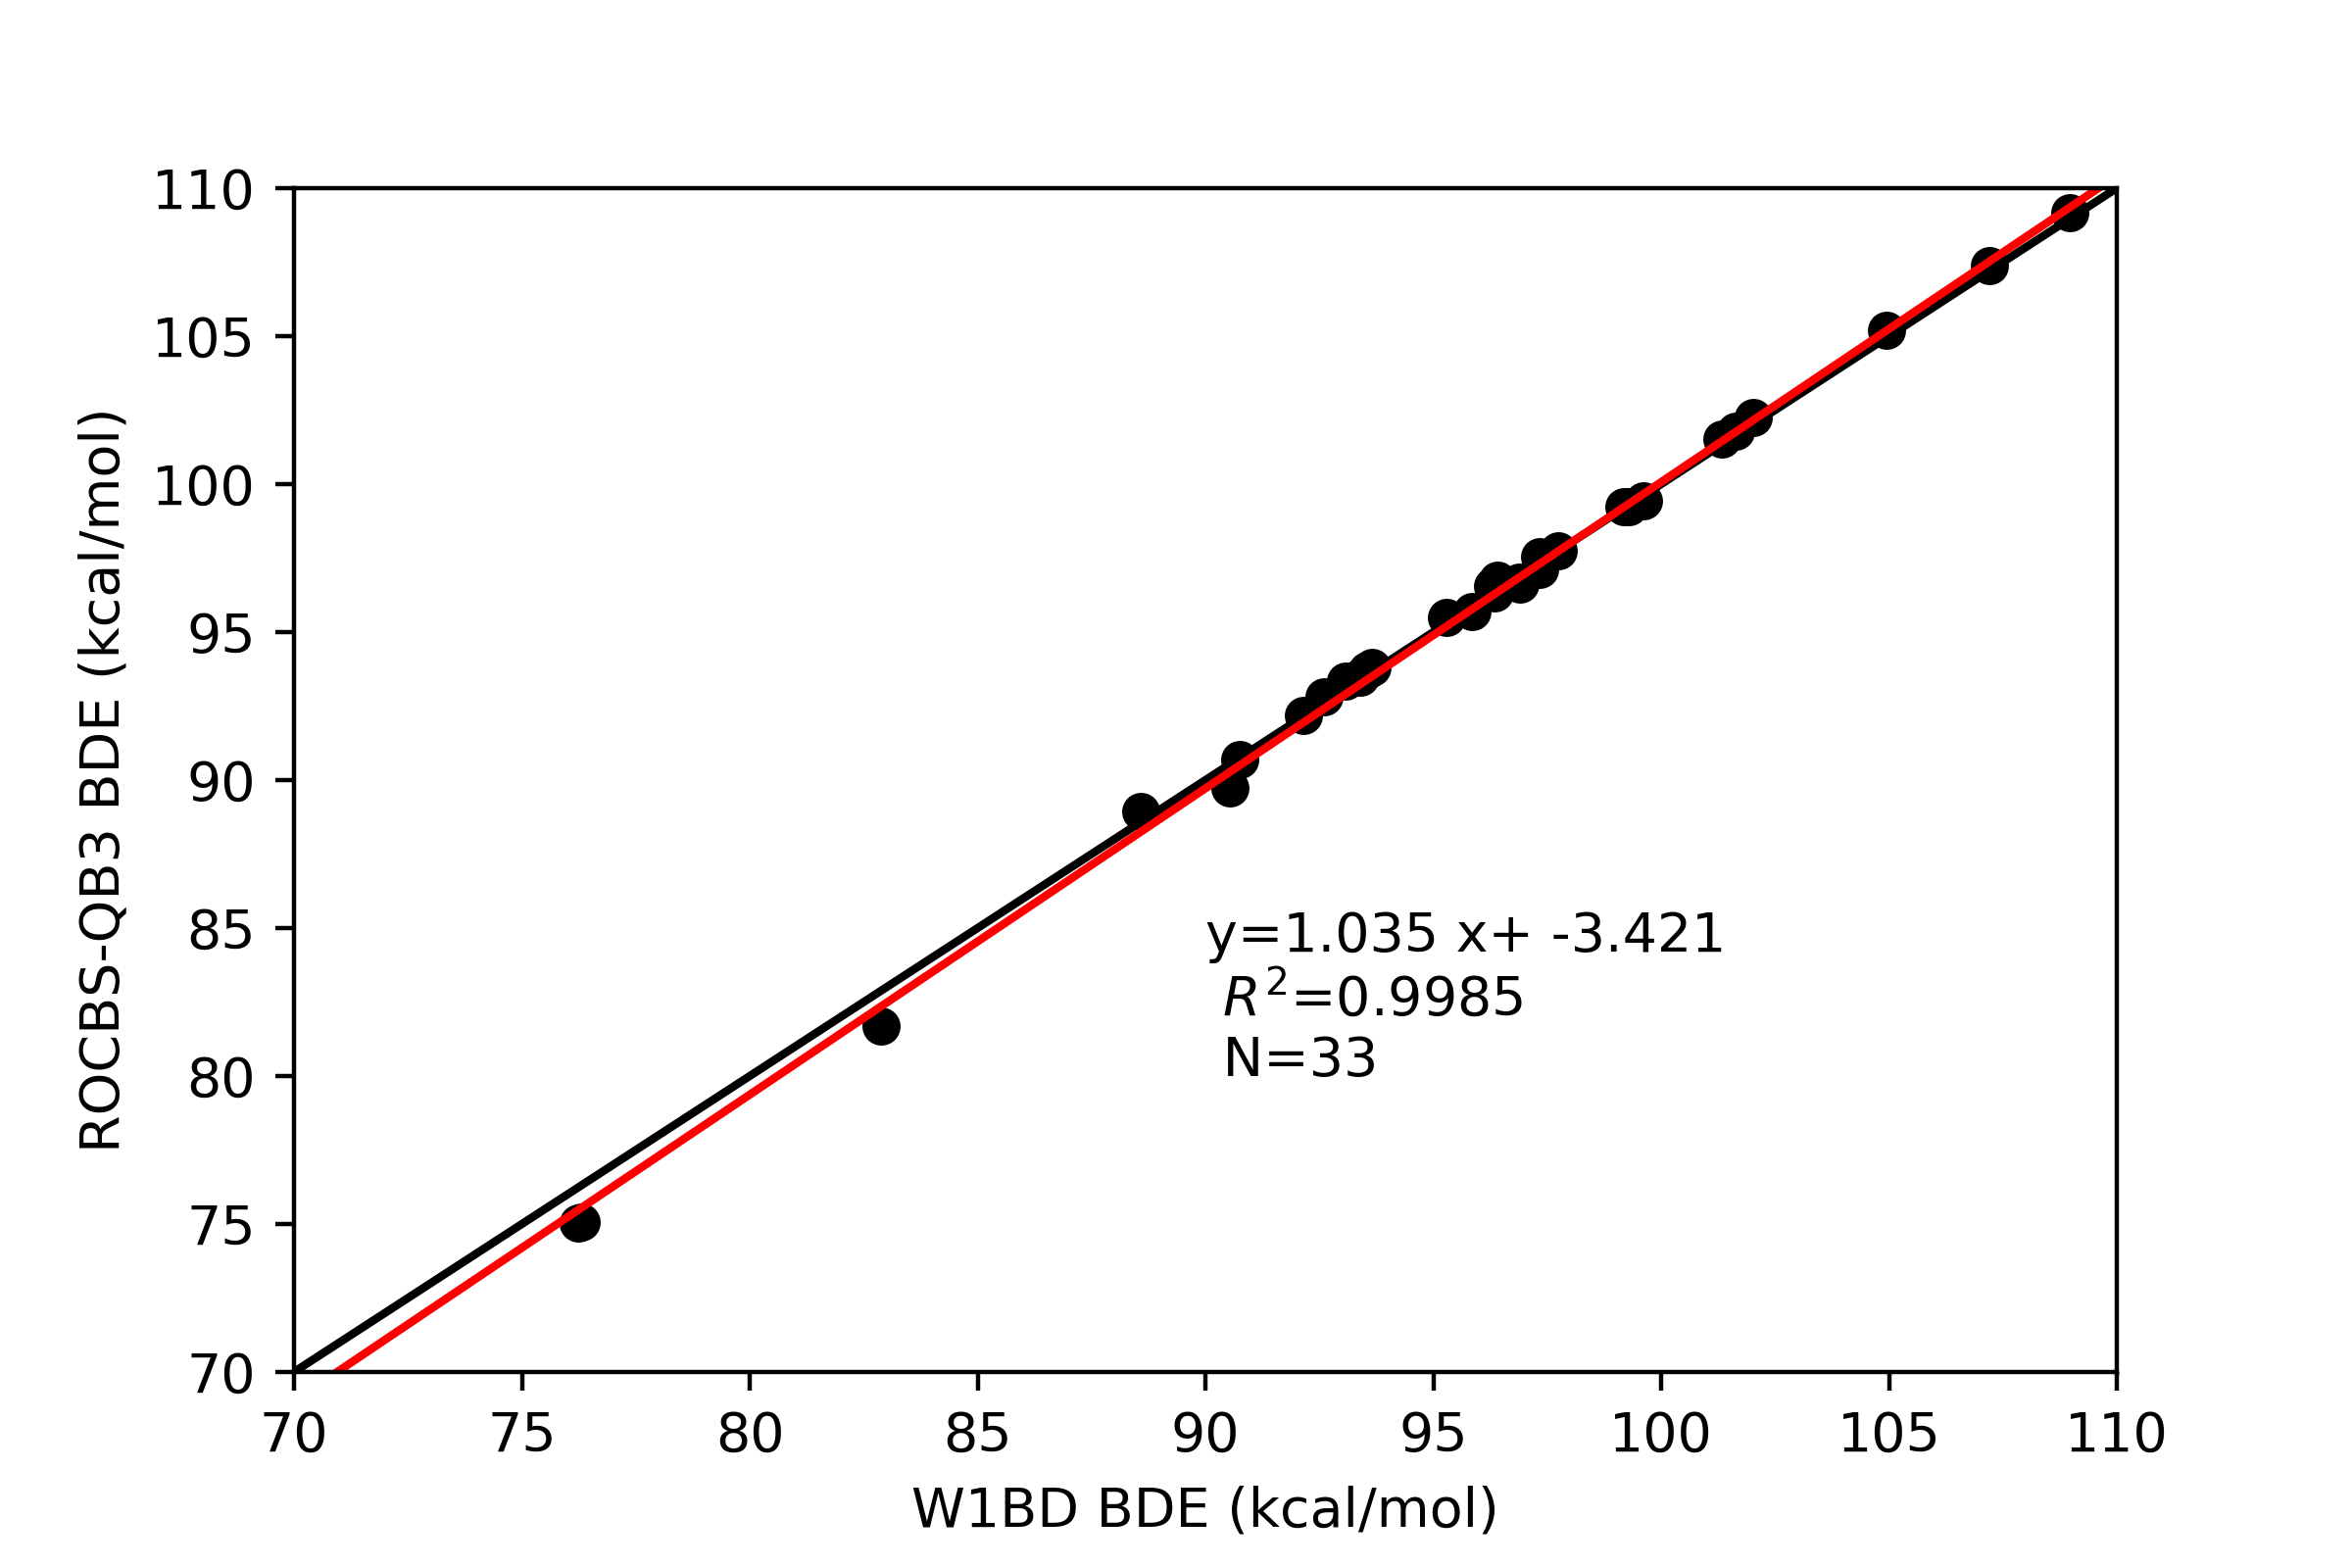
\includegraphics[width=\textwidth]{figures/w1bd-rocbsqb3}
  \end{minipage}
  \caption[One-to-one plot comparing calculated BDEs calculated by ROCBS-QB3 to literature and W1BD BDEs.]{One-to-one plot comparing calculated BDEs calculated by the ROCBS-QB3 to reference literature\protect\cite{Luo2002} and W1BD BDE values, respectively. The red line represents the least squares line of best fit, while black line represents a perfect one-to-one correlation.}
  \label{fig:1-1-ROCBSQB3}
\end{figure}

In summary, ROCBS-QB3 performs best for the calculation of \ch{C-H} BDEs while G4(MP2) performs worst. Given these data, and considering the relative computational cost, the ROCBS-QB3 method is recommended for the calculation of accurate BDEs, particularly for large molecules for which more expensive computational methods are not possible. Importantly, we can now confidently continue investigating the BEP relationships using reliable calculated BDE data from the ROCBS-QB3 method. Furthermore, these results can be extended to even larger systems as the ROCBS-QB3 approach is one of the least computationally expensive composite methods. For example, for calculations on the cyclohexane molecule, which take about 20 minutes using ROCBS-QB3 on SGI Altix compute nodes with 6 processors and 8 GB RAM, while G4 takes about 27 times longer, the LDBS approach takes about 500 times longer, and W1BD takes about 1100 times longer.

\section{Analysis of the Bell-Evans-Polanyi principle}

We turn now to the application of accurate BDEs to the BEP principle. Experimental HAT rate constants have been collected for 32 reactions involving \cumo and organic substrates. The BEP plot of the logarithm of rate constants divided by the number of equivalent H atoms (i.e. normalised) against BDEs is shown in~\ref{fig:bde-bep}.

\begin{figure}[!htbp]
  \centering
  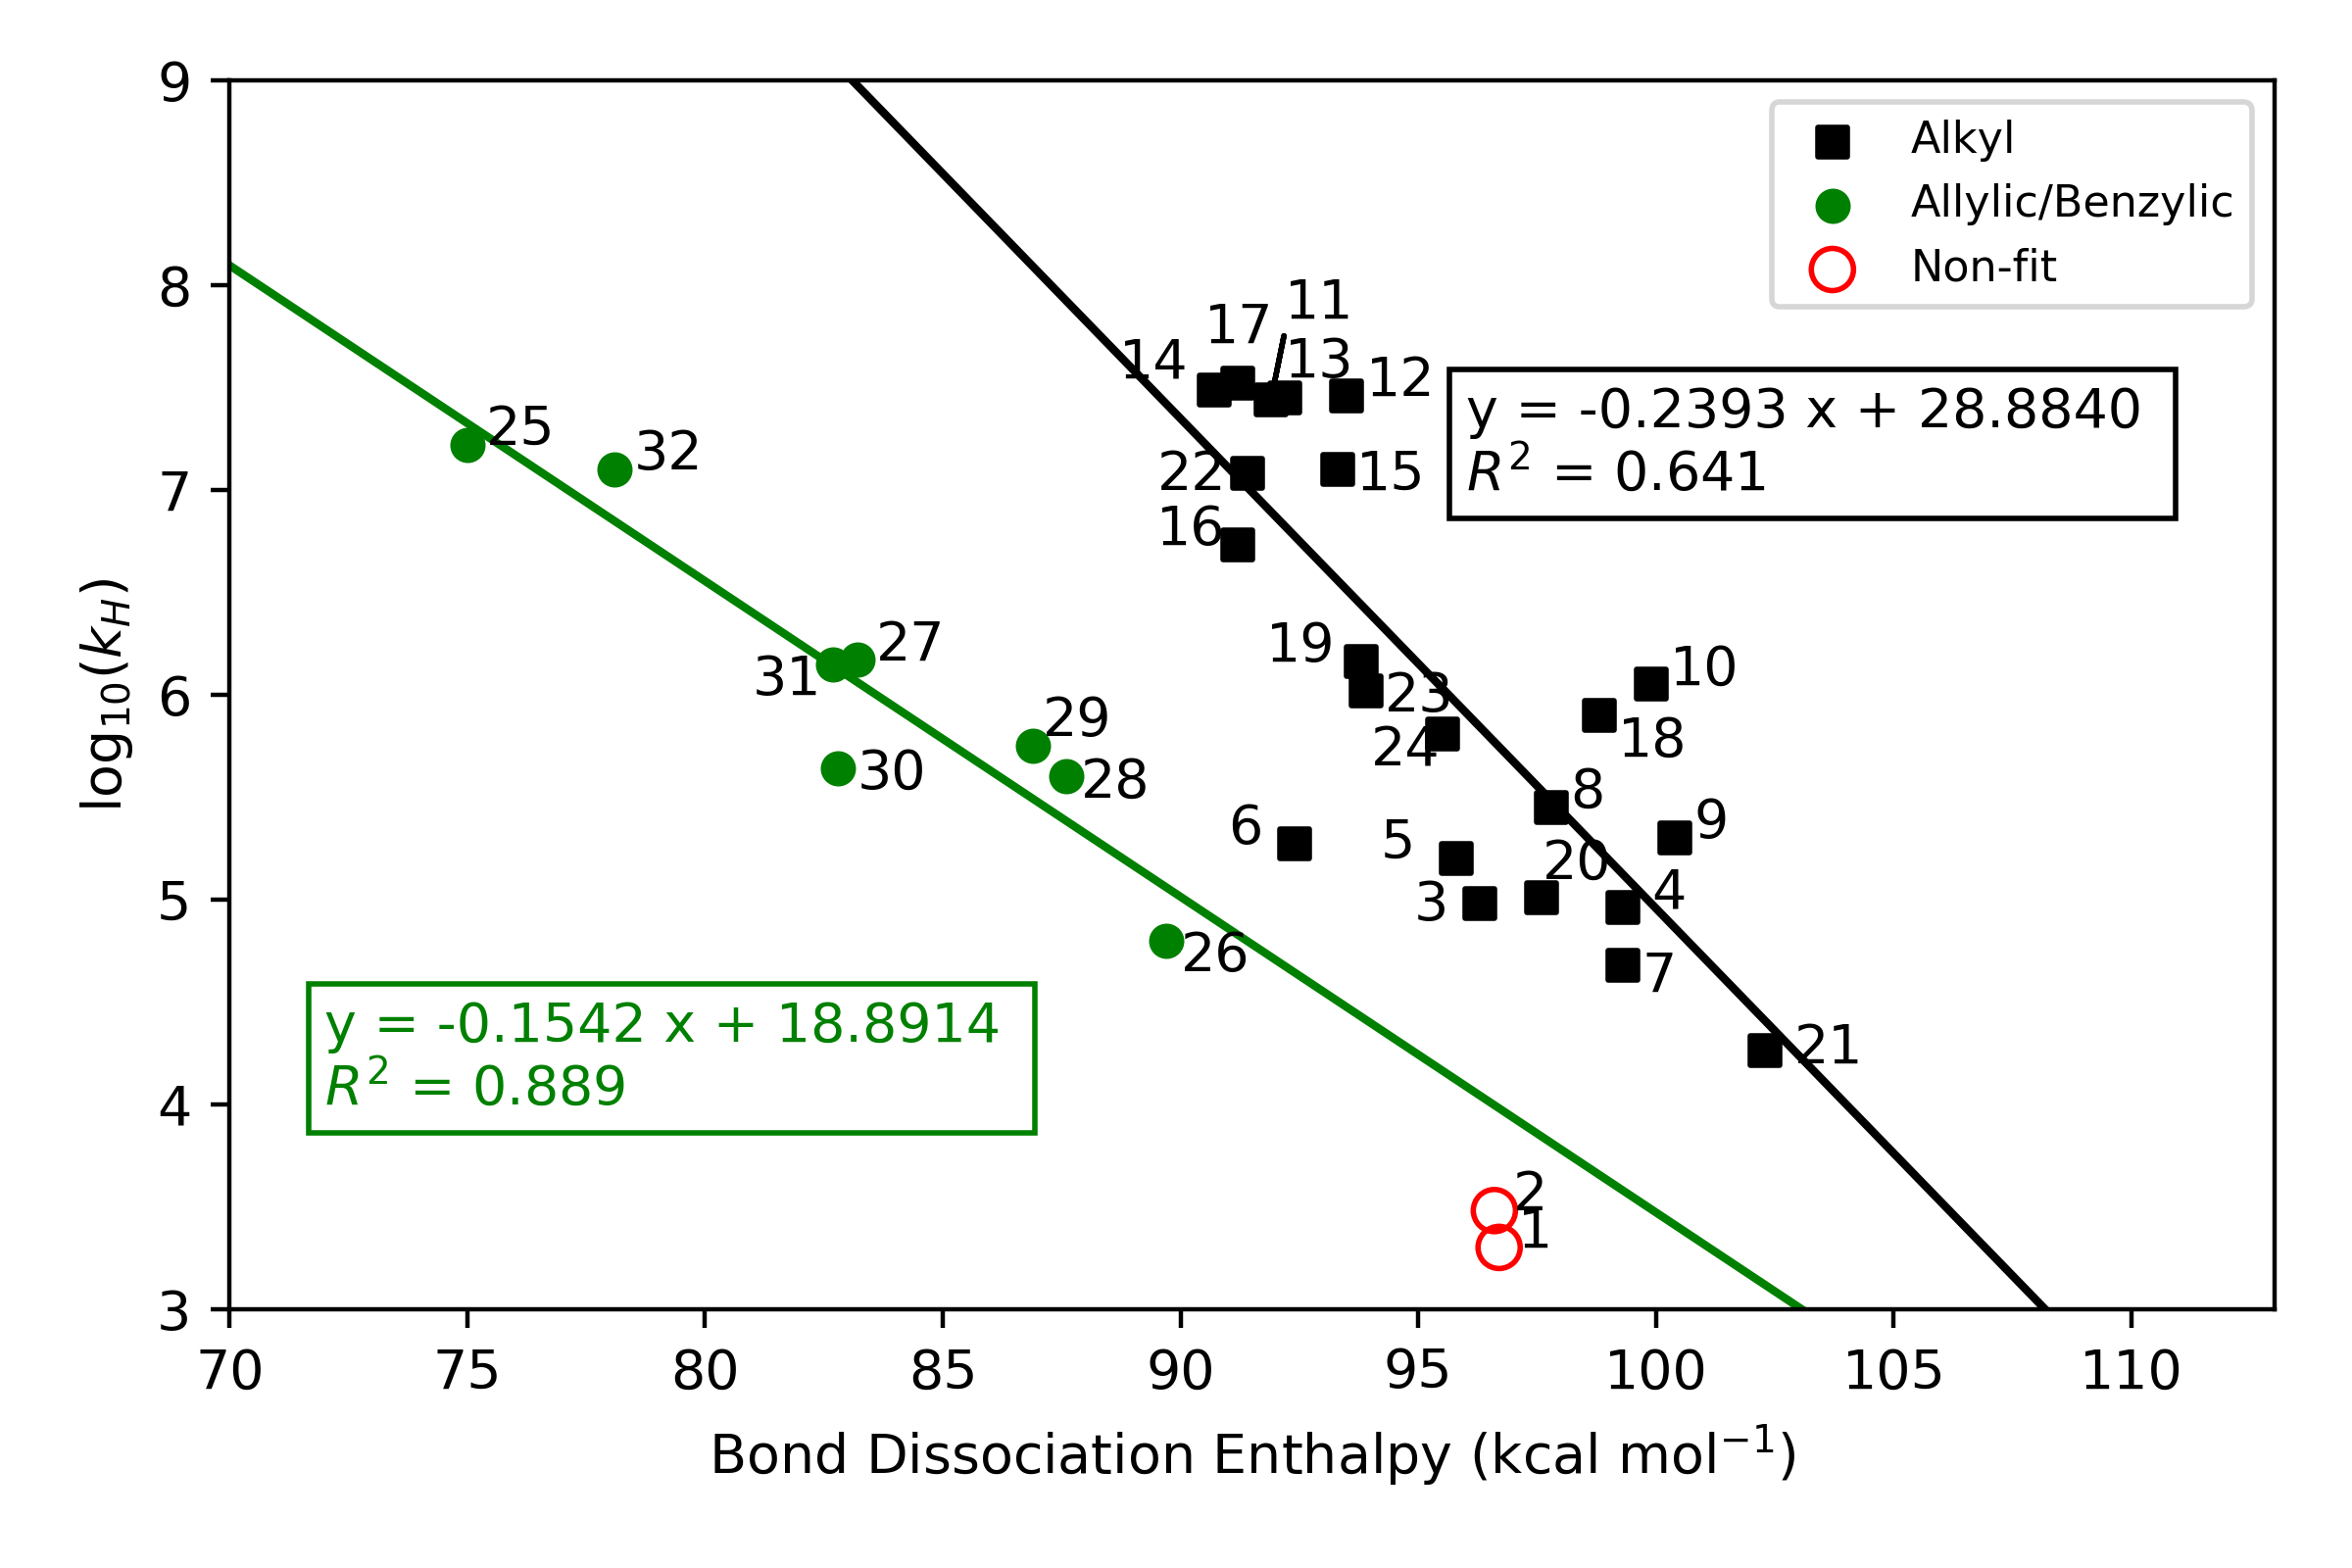
\includegraphics[width=\textwidth]{figures/bde-bep}
\begin{tabularx}{\textwidth}{| l X l X |}
  \hline
  1 & Acetone & 2 & Acetonitrile \\
  3 & Cyclopentane & 4 & Cyclohexane \\
  5 & Cycloheptane & 6 & Cyclooctane \\
  7 & 2,2-dimethylbutane & 8 & 2,3-dimethylbutane \\
  9 & Adamantane (2$^\circ$) & 10 & Adamantane (3$^\circ$) \\
  11 & Diethyl amine & 12 & Piperazine \\
  13 & Piperidine & 14 & Pyrrolidine \\
  15 & Morpholine & 16 & Propylamine \\
  17 & Triethylamine & 18 & 1,4-diazobicyclo[2.2.2]octane \\
  19 & Tetrahydrofuran & 20 & Dioxane \\
  21 & Dimethyl sulfoxide & 22 & Benzaldehyde \\
  23 & Hexamethylphosphoramide & 24 & Diethyl ether \\
  25 & 1,4-cyclohexadiene & 26 & Toluene \\
  27 & Benzyl alcohol & 28 & Ethylbenzene \\
  29 & Cumene & 30 & Diphenylmethane \\
  31 & Dibenzyl ether & 32 & 9,10-dihydroanthracene \\
  \hline
\end{tabularx}
  \caption[Bell-Evans-Polanyi plot of experimental rate constants (normalised for the number of equivalent hydrogen atoms) for HAT between \cumo~ and substrates against BDEs calculated using the ROCBS-QB3 method.]{Bell-Evans-Polanyi plot of experimental rate constants (normalised for the number of equivalent hydrogen atoms) for HAT between \cumo~ and substrates against BDEs calculated using the ROCBS-QB3 method.. Acetone and acetonitrile are note included in fitting as the experimental rate constants are approximate.}
\label{fig:bde-bep}
\end{figure}

As with the experimental results in~\ref{fig:bep-expt}, there clearly exists two distinct regions in~\ref{fig:bde-bep}. This is inline with our initial hypothesis that there should exist two linear relations: one for allylic/benzylic C-H bonds, and another for alkyl C-H bonds. However, there remains a considerable amount of scatter in the data, thus correlation of the expected BEP relations is poor. For the allylic/benzylic series of C-H BDEs which result in a radical which is delocalised, the correlation coefficient is 0.89. This result is consistent with work of Pratt et al.\cite{Pratt2003}, which found a BEP plot correlation coefficient of 0.82 for the abstraction of C-H bonds from model unsaturated fatty acids. Most of the rate constants used in the work of Pratt et al. are for the abstraction of \ch{C-H} by peroxyl radicals, which were obtained through an experimental method which gives estimated HAT rate constants with large associated errors. Thus, they suggested that the degree of scatter is associated with experimental errors. The same however, cannot be said for the rate constants associated with this work. Therefore, there must be additional physico-chemical factors at play.

The alkyl C-H BDEs show very weak correlation with \cumo~ HAT rate constants, with a correlation coefficient of 0.63. One possibility is that applying the BEP principle to such a large grouping of substrates is inappropriate. Thus, I have replotted this data in~\ref{fig:bep-breakdown}, breaking the data into several smaller chemical groupings: cyclic alkanes, other alkanes, tertiary amines (Tert. Amines), hydrogen bond donating (H-Bond Donors) species, and other \ch{C-H} bonds with heteroatom neighbours (Het. Neighbours). Doing so appears to reveal one well correlated trend for \ch{C-H} bonds with heteroatom neighbours ($R^2 = 0.96$). There are two data points for the tertiary amines, thus the points should not be fit to a line, however it is unclear why they do not fit into the other heteratomic neighbours trend. The cyclic alkanes are poorly correlated ($R^2 = 0.73$). Extremely poor correlation is observed for both the hydrogen bond donating species and other alkanes. There are no evident reasons on the basis of substrate structures which explains the poor correlations observed. Thus, the lack of simple relationships is perhaps evidence against the validity of the BEP principle. However, before making any conclusions, we must consider if there are any explanations that arise from examining the transition state structures.

\begin{figure}[!htbp]
  \centering
  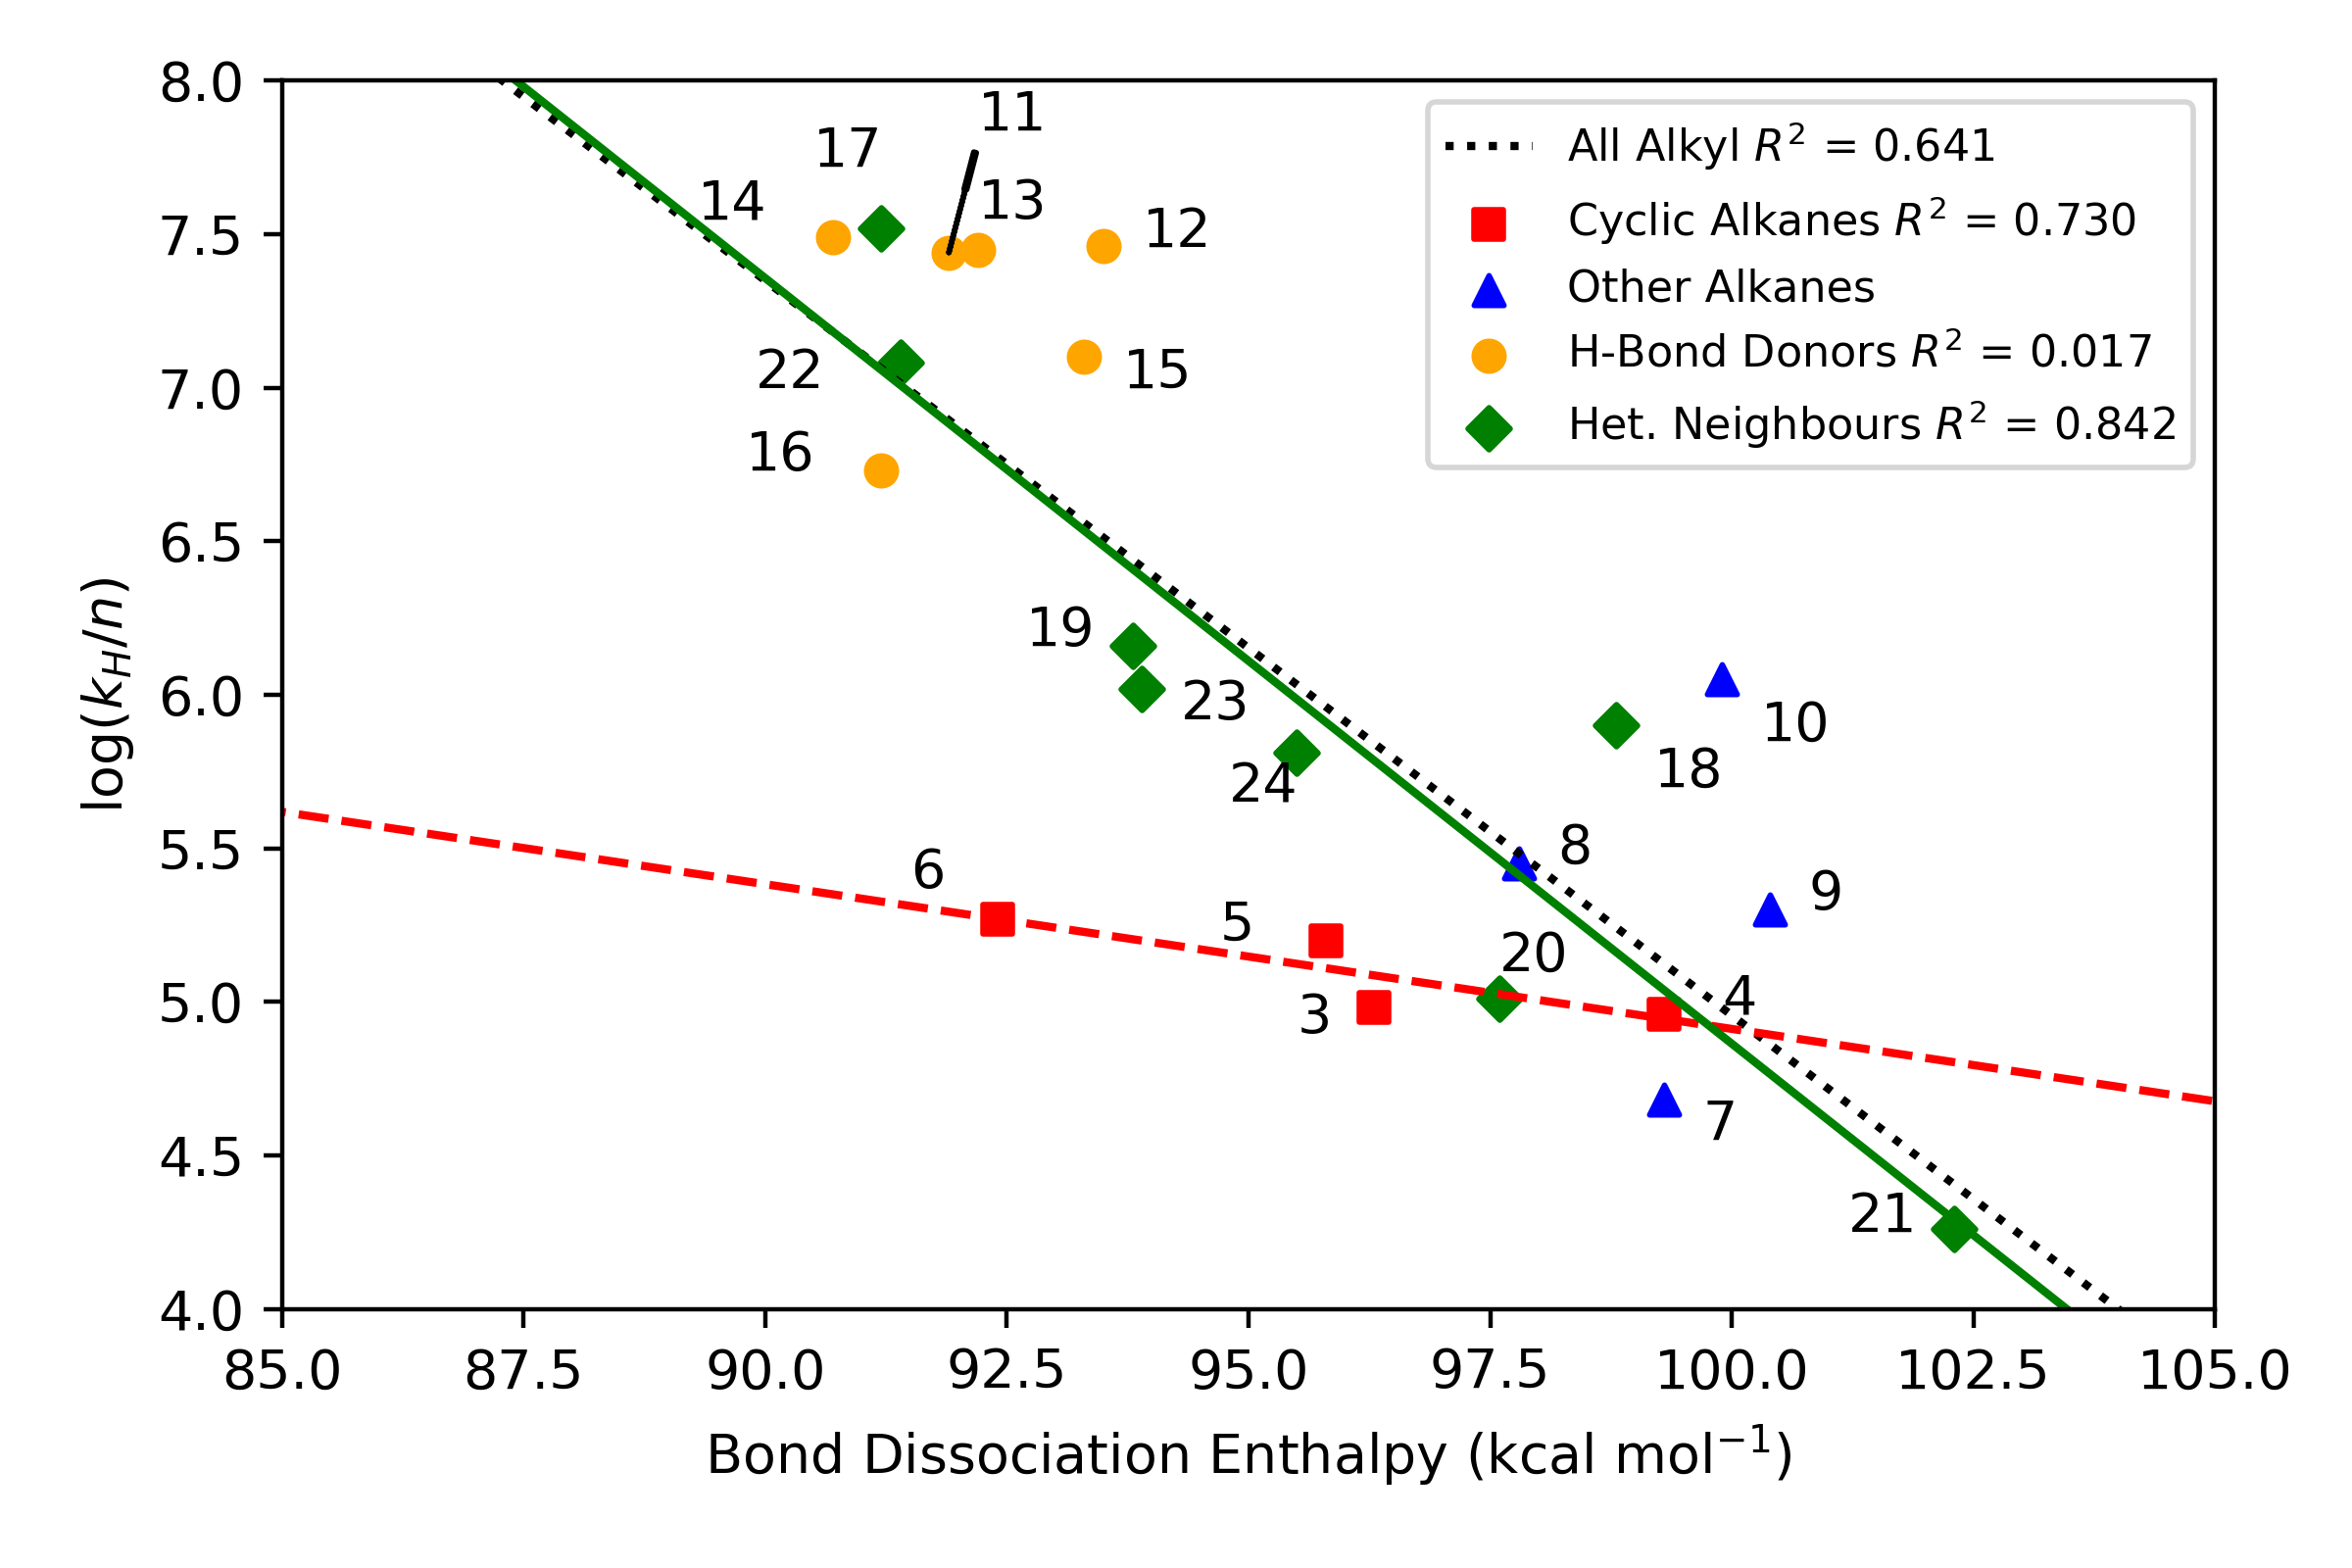
\includegraphics[width=\textwidth]{figures/bep-breakdown}
  \begin{tabularx}{\textwidth}{| l X l X |}
    \hline
    3 & Cyclopentane & 4 & Cyclohexane \\
    5 & Cycloheptane & 6 & Cyclooctane \\
    7 & 2,2-dimethylbutane & 8 & 2,3-dimethylbutane \\
    9 & Adamantane (2$^\circ$) & 10 & Adamantane (3$^\circ$) \\
    11 & Diethyl amine & 12 & Piperazine \\
    13 & Piperidine & 14 & Pyrrolidine \\
    15 & Morpholine & 16 & Propylamine \\
    17 & Triethylamine & 18 & 1,4-diazobicyclo[2.2.2]octane \\
    19 & Tetrahydrofuran & 20 & Dioxane \\
    21 & Dimethyl sulfoxide & 22 & Benzaldehyde \\
    23 & Hexamethylphosphoramide & 24 & Diethyl ether \\
    \hline
  \end{tabularx}
  \caption[Further breakdown of Bell-Evans-Polanyi plot of experimental rate constants (normalised for the number of equivalent hydrogen atoms) for HAT between \cumo~ and alkyl substrates against BDEs calculated using the ROCBS-QB3 method.]{Further breakdown of Bell-Evans-Polanyi plot of experimental rate constants (normalised for the number of equivalent hydrogen atoms) for HAT between \cumo~ and  substrates.}
\label{fig:bep-breakdown}
\end{figure}

\newpage
\section{Transition state analysis}

In order to determine if there are any reasons for the breakdown of the BEP principle, I have calculated TS structures for 20 of the reactions at the LC-$\omega$PBE-D3(BJ)/6-311+G(2d,2p)//B3LYP-D3(BJ)/6-31+G$^*$ level of theory. The calculated reaction free-energy barrier heights ($\Delta G^\ddagger$) are listed in~\ref{tab:ts-bep}, along with the decomposition into enthalpic and entropic terms: $\Delta G^\ddagger = \Delta H^\ddagger - T\Delta S^\ddagger$.

\begin{table}[!htbp]
  \caption[Reaction barrier heights for reactions of substrates with \cumo calculated in the gas phase at 298 K.]{Reaction barrier heights for reactions of substrates with \cumo calculated in the gas phase at 298 K at the LC-$\omega$PBE-D3(BJ)/6-311+G(2d,2p)//B3LYP-D3(BJ)/6-31+G$^*$ level of theory. All values are in units of \kcalmol. ID numbers match those in~\protect\ref{fig:bde-bep}\ $^\dagger$TS structure contains small additional imaginary frequency.}
  \label{tab:ts-bep}
  \begin{tabular}{l l c c c}
    ID & Substrate & $\Delta G^\ddagger$ & $\Delta H^\ddagger$ & $-T\Delta S^\ddagger$ \\
    \hline
    \multicolumn{5}{c}{\textbf{Non-fit}}\\
    1 & Acetone & 17.6 & 3.6 & 14.0 \\
    2 & Acetonitrile & 18.3 & 6.8 & 11.5 \\
    \hline
    \multicolumn{5}{c}{\textbf{ Cyclic Alkanes}}\\
    3 & Cyclopentane$^\dagger$ & 13.5 & 0.5 & 13.0 \\
    4 & Cyclohexane & 11.8 & 1.2 & 10.6 \\
    6 & Cyclooctane$^\dagger$ & 13.6 & -0.5 & 14.1 \\
    \hline
    \multicolumn{5}{c}{\textbf{Other Alkanes}}\\
    7 & 2,2-dimethylbutane & 11.2 & -0.8 & 12.0 \\
    8 & 2,3-dimethylbutane & 11.2 & 1.1 & 10.2 \\
    9 & Adamantane (2$^\circ$) & 12.6 & 0.6 & 12.0 \\
    10 & Adamantane (3$^\circ$) & 10.8 & -1.0 & 11.8 \\
    \hline
    \multicolumn{5}{c}{\textbf{Tert. Amine and H-Bond Donor}} \\
    11 & Diethylamine & 10.0 & -3.0 & 13.0 \\
    18 & 1,4-diazobicyclo[2.2.2]octane & 11.8 & -0.5 & 12.3 \\
    \hline
    \multicolumn{5}{c}{\textbf{Heteroatom Neighbours}} \\
    20 & Dioxane & 11.4 & -0.4 & 11.8 \\
    21 & Dimethyl sulfoxide & 15.7 & 3.8 & 11.9 \\
    22 & Benzaldehyde$^\dagger$ & 12.6 & -0.3 & 12.9 \\
    23 & Hexamethylphosphoramide & 12.1 & -2.3 & 14.4 \\
    24 & Diethyl ether & 7.6 & -3.8 & 11.4 \\
    \hline
    \multicolumn{5}{c}{\textbf{Allylic/Benzylic}}\\
    25 & 1,4-cyclohexadiene & 12.0 & -1.0 & 13.0 \\
    26 & Toluene & 14.7 & 0.9 & 13.7 \\
    29 & Cumene & 11.4 & -1.9 & 13.3 \\
    30 & Diphenylmethane$^\dagger$ & 13.6 & -1.0 & 14.5 \\
    32 & 9,10-dihydroanthracene$^\dagger$ & 11.4 & -3.2 & 14.6 \\
  \end{tabular}
\end{table}

First, consider some general features associated with the TS complexes listed in~\ref{tab:ts-bep}. One factor which may lead to deviations from the BEP is the possibility for different HAT reaction mechanisms, i.e. direct HAT or PCET. Consider first the reaction of toluene with \cumo. As this reaction is similar to the self-exchange reaction of the benzyl-toluene couple as described by DiLabio and Johnson,\cite{DiLabio2007} one might expect the reaction to proceed via PCET. The lowest energy TS complex has a partially $\pi$-stacked conformation with the rings oriented about 40$^\circ$ relative to one another. Examination of the SOMO and HOMO reveals no $\pi$-$\pi$ partial bonding interaction, as can be seen in~\ref{fig:cumo-toluene}. The electron density of the SOMO is largely localised on the toluene portion of the complex. This is likely due to the additional non-conjugated carbon centre of \cumo, which prevent an additional electron channel for PCET to occur. Therefore, this reaction takes place through direct HAT, as has been previously described.\cite{Salamone2011} This behaviour is specific to the \cumo~ radical, thus all the reactions likely also take place through a direct HAT mechanism, and this should not factor into the deviations in the observed BEP principle relationships.

\begin{figure}[!htbp]
\centering
\hspace*{-1.8cm}
\begin{minipage}{8cm}
  \centering
  \begin{overpic}[width=\textwidth]{figures/cumo-tol-somo}
  \put(5,100) {\large\textbf{A.}}
\end{overpic}
\end{minipage}%
\begin{minipage}{8cm}
  \centering
  \begin{overpic}[width=\textwidth]{figures/cumo-tol-homo}
  \put(5,100) {\large\textbf{B.}}
\end{overpic}
\end{minipage}
\caption[Structures of TS for HAT between \cumo and toluene with SOMO and HOMO.]{Structures of TS for HAT between \cumo and toluene with \textbf{A.} SOMO and \textbf{B.} HOMO. The elements are coloured as grey for carbon, white for hydrogen, and red for oxygen.}
\label{fig:cumo-toluene}
\end{figure}

For all of the TS structures of the reactions in~\ref{tab:ts-bep}, a conformation which maximises non-covalent interactions while minimising steric repulsion is adopted. In the cases of acetone, acetonitrile, hexamethylphosphoramide (HMPA), and DMSO, a very weak hydrogen bonding interaction is formed between the \ch{X=O} (or \ch{C+N} for acetonitrile) moieties and the C-H of the methyl of \cumo. In all but two cases, this involves a cisoid (partially stacked) complex so that dispersion interactions are maximised. The two outliers are benzaldehyde and cyclooctane. In order for benzaldehyde to adopt a cisoid TS structure, there are two possibilities. First, a T-shaped conformation could be adopted, rather than a slipped-parallel $\pi$-stacked conformation. On the basis of the benzene-benzene non-covalently bound dimer,\cite{Sinnokrot2002} this conformation is very slightly favourable by circa 0.1 \kcalmol. However, this would require a rotation of nearly 90$^\circ$ of the \ch{C(CH3)2O^.} of \cumo, which has an energetic cost\footnotemark~ of 4.3 \kcalmol, thus this conformation is unlikely. On the other hand, the \ch{C(CH3)2O^.} of \cumo could rotate to accommodate a partially slipped-parallel $\pi$-stacking conformation in the TS complex. Note that I was unable to obtain TS structures for either of the described possible cisoid conformations for the benzaldehyde-\cumo TS complex. For cyclooctane, the difference in free energy between the cisoid and transoid TS structures is 1.8 \kcalmol, however both structures were unable to be fully optimised and contain a secondary small imaginary frequency. The reason for favouring a transoid TS structure is somewhat unclear, but it is possible that the non-optimal nature of the TS structures is the cause. Furthermore, it is possible that the cyclooctane molecule undergoes a conformational change in forming the TS complex which was not accounted for in these calculations. Cyclooctane has many conformations which are close in relative energy.\cite{Dorofeeva1985}

\footnotetext{Calculated at the LC-$\omega$PBE-D3(BJ)/6-311+G(2d,2p) level of theory.}

TS complex structures and mechanism aside, there is one striking features in the reaction barriers calculated for HAT reactions involving \cumo: all the the reactions studied are entropy-controlled at 298 K. This means that the free-energy barrier, and thus rate constant, is controlled by the entropic contributions, rather than the enthalpic contributions, i.e. $-T\Delta S^\ddagger > \Delta H^\ddagger$. From the results in~\ref{tab:ts-bep}, it can be said that $-T\Delta S^\ddagger >> \Delta H^\ddagger$ for hydrogen abstraction by \cumo. One interpretation of these results is that \cumo~ is so highly reactive, that HAT is governed by trajectory, orientation, and degrees of freedom, factors that are normally associated with the A-factor in Arrhenius theory. In fact, in many cases, $\Delta H^\ddagger$ is calculated to be negative with respect to the separated reactants. This implies that a pre-reaction complex is formed, which as was demonstrated in Chapter~\ref{ch:arrhenius}, can have significant importance on HAT reactivity with respect to the magnitude of the A-factor. Pre-reaction complex structures were not calculated in this work, however  in some cases the systems have been studied in combined experimental and theoretical work. Some examples of previously calculated \cumo + substrate pre-reaction complex binding enthalpies are: HMPA\footnotemark\ $\Delta H \approx$ -6 \kcalmol, DMSO $\Delta H \approx$ -5 \kcalmol, and 1,4-diazobicyclo[2.2.2]octane (DABCO)\cite{Salamone2011b} $\Delta H \approx$ -0.1 \kcalmol. Note that the calculated enthalpic barrier herein is -0.5 \kcalmol~ for DABCO, a result which can be ascribed to differences in computational methods. In Ref.~\citenum{Salamone2011b}, no dispersion correction was used, thus accounting for a less stable TS complex and pre-reaction complex. The calculated difference in enthalpy from pre-reaction complex to TS complex for DABCO was found to be only 1.0 \kcalmol.

\footnotetext{DMSO and HMPA were studied in Ref. \citenum{Salamone2012} at the B3LYP-DCP\cite{Torres2012}/6-31+G(2d,2p) level of theory}

The fact that hydrogen abstraction by \cumo is entropy-controlled is perhaps unsurprising, given the work of \citet{Finn2004}, that demonstrated that HAT reactions involving various organic substrates and the closely related radical \ch{$t$-BuO^.} are also entropy-controlled at room temperature. Furthermore, it has been shown that \cumo and \ch{$t$-BuO^.} display very similar hydrogen atom abstraction reactivities.\cite{Salamone2011, Valgimigli1995, Sheeller2001, Baignee1983} It is surprising then that these radicals remain so often applied as proxies for reactive oxygen species in kinetic studies. Future work should use extreme caution in applying \cumo~ and \ch{$t$-BuO^.} as chemical probes, as been noted in the past.\cite{Finn2004, Salamone2011b, Salamone2011} Note also, that it is uncommon to encounter entropy-controlled reactions in organic chemistry, and are often associated with non-Arrhenius behaviour. Other examples of reported entropy-controlled reactions include the addition of a carbene across a multiple bond,\cite{Houk1984, Moss2017} and radical-radical recombination reactions.\cite{Sobek2001}

Classical physical organic chemical literature can explain why the reactions which are entropy-controlled do not follow ``normal'' LFERs.\cite{Exner1973} \citet{Blackadder1958} defined three classifications for different types of LFERs, the first of which applies to the BEP principle: A series of reactions with constant entropy are controlled by enthalpy changes which are based on electronic effects that do not affect the form of the TS. Therefore, reaction rates which involve non-isoentropic TS complex formation will not correlate with bond strengths, as is observed herein. It seems prudent at this point to suggest that expecting reactions to be isoentropic with respect to transition state formation is an over-simplification, especially given the number of factors which contribute to entropy in solvent phase chemistry.

\section{Is the Bell-Evans-Polanyi principle valid?}

The question still remains if the BEP principle is valid or not. Recall from Equation~\ref{eq:Ea-vs-dH} that $E_a$ is related directly to $\Delta H^\ddagger$. Thus, if the BEP principle still holds for HAT reactions between \cumo and organic substrates, then the calculated values of $\Delta H^\ddagger$ should be a function of \ch{C-H} BDE. These data are plotted in~\ref{fig:bep-dG}.

\begin{figure}[!htbp]
  \centering
  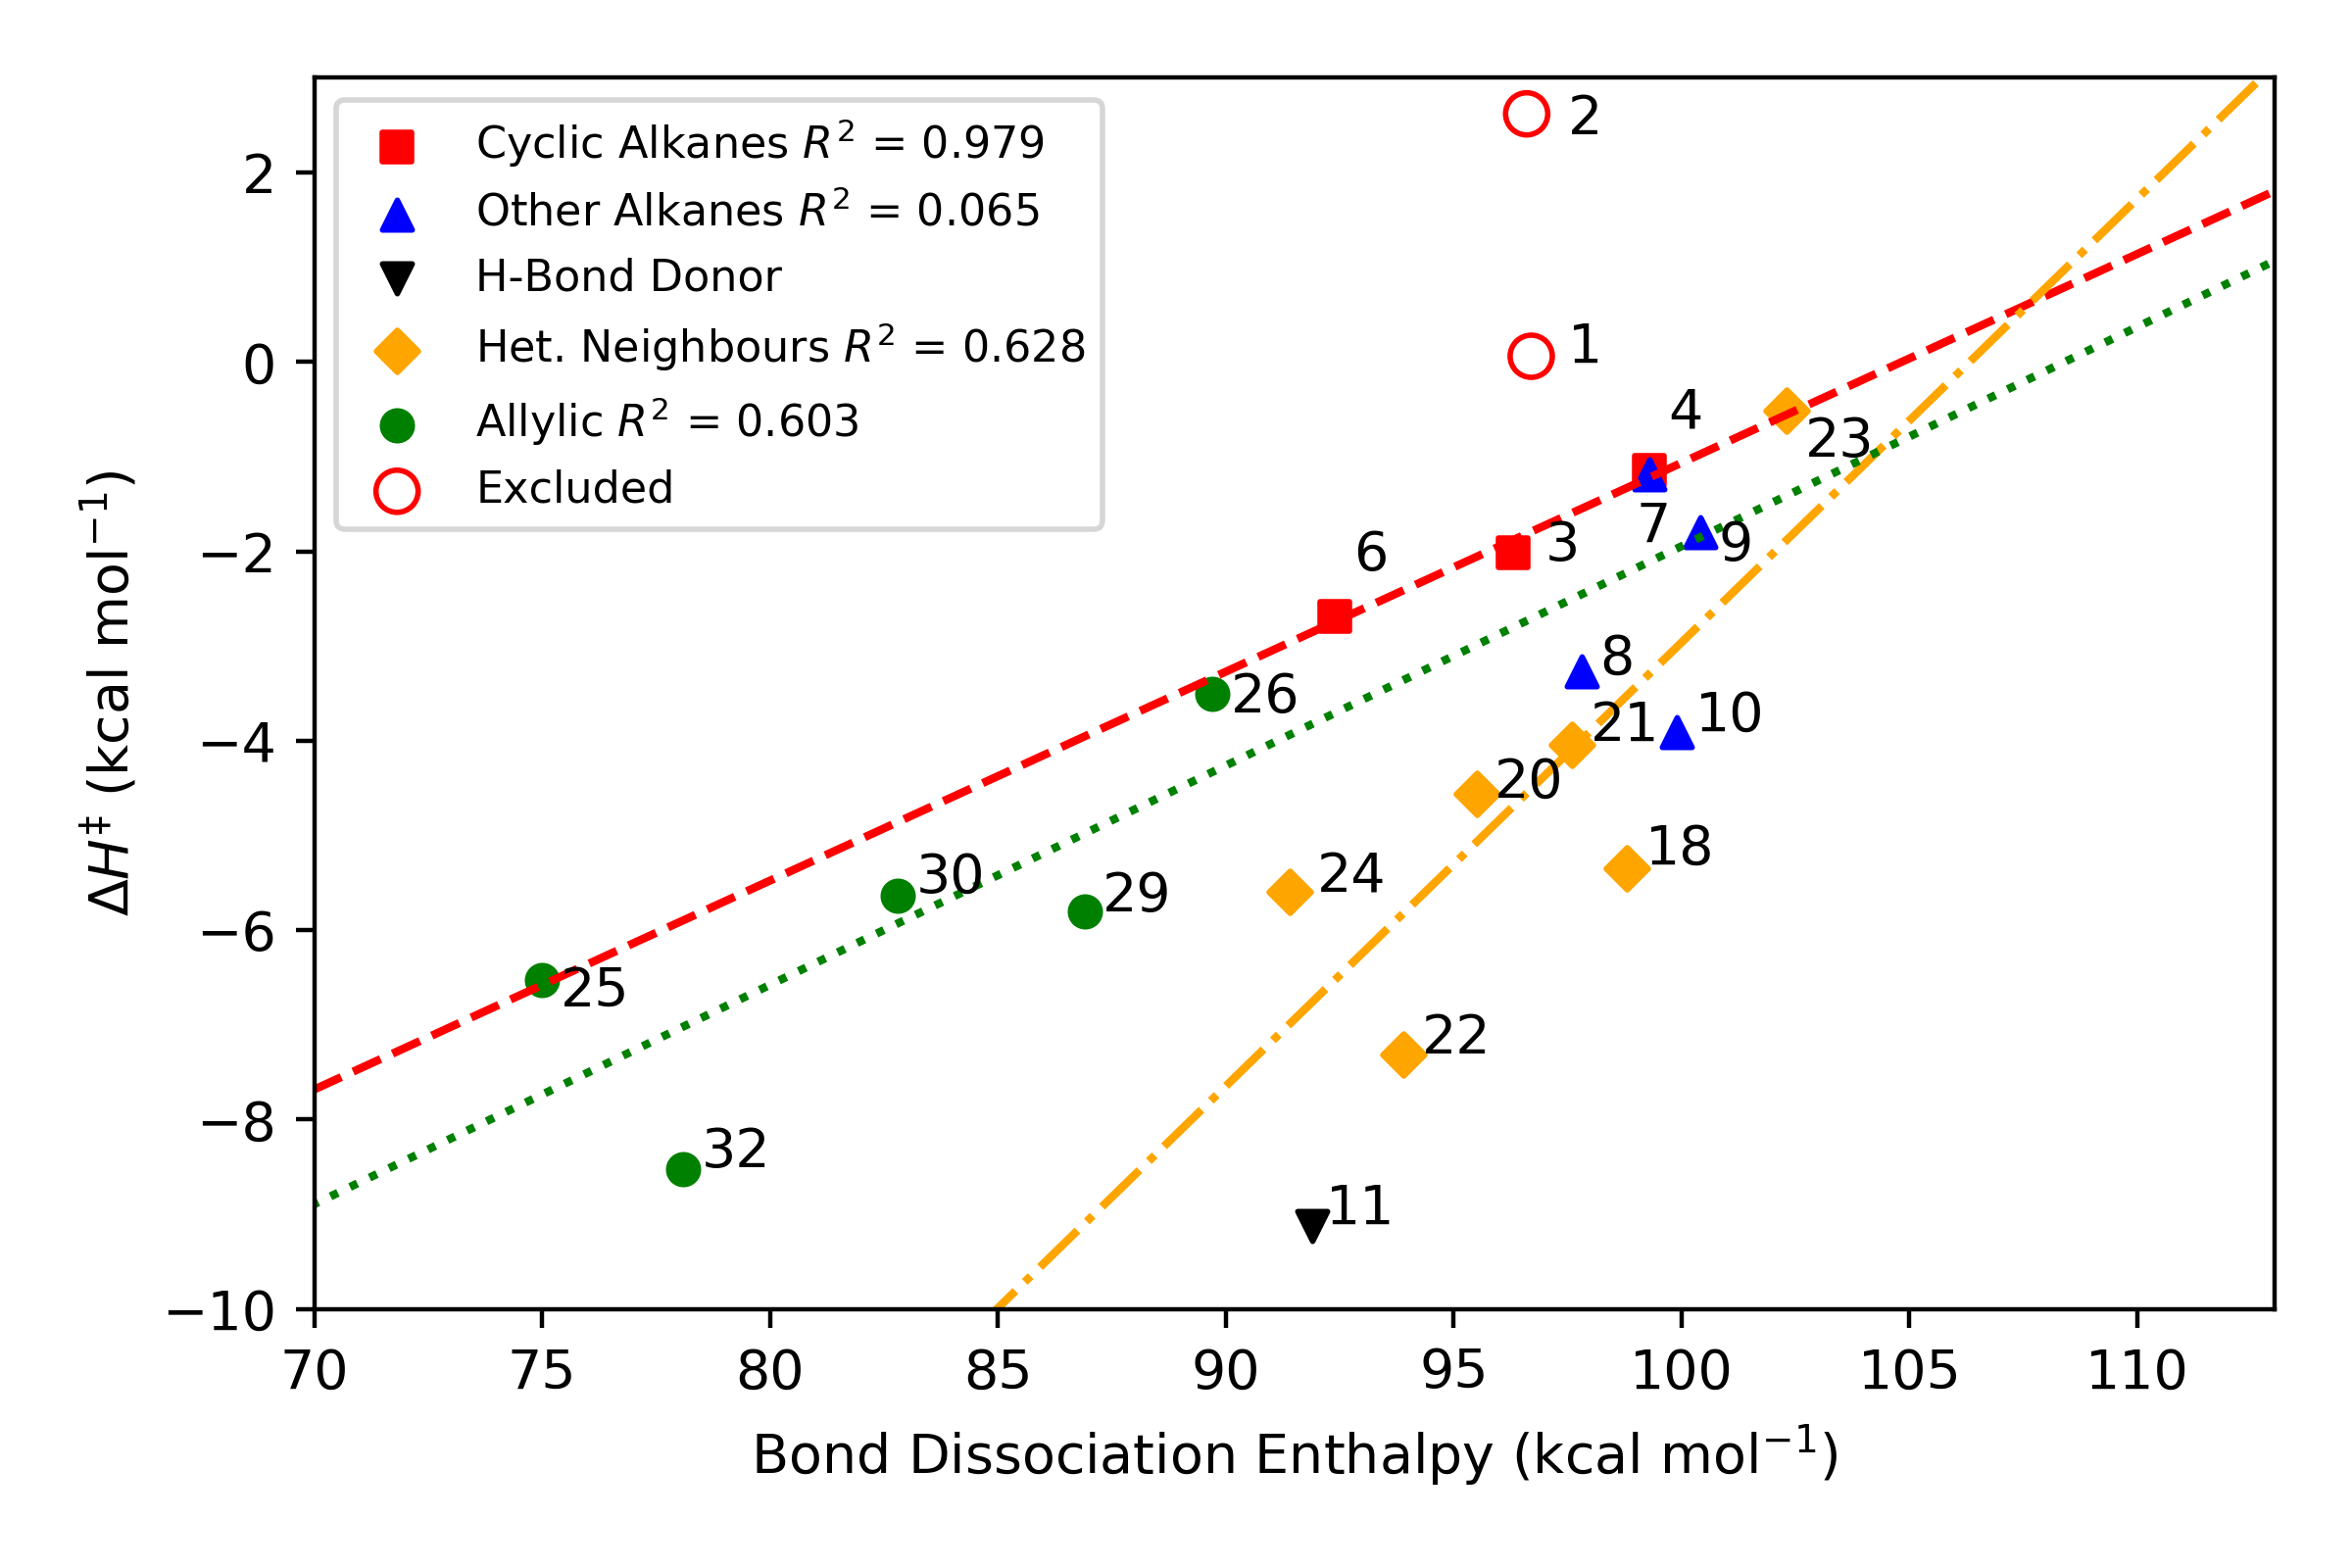
\includegraphics[width=\textwidth]{figures/bep-dG}
\begin{tabularx}{\textwidth}{| l X l X |}
  \hline
  1 & Acetone & 2 & Acetonitrile \\
  3 & Cyclopentane & 4 & Cyclohexane \\
  6 & Cyclooctane & 7 & 2,2-dimethylbutane \\
  8 & 2,3-dimethylbutane & 9 & Adamantane (2$^\circ$) \\
  10 & Adamantane (3$^\circ$) & 11 & Diethyl amine \\
  18 & 1,4-diazobicyclo[2.2.2]octane & 20 & Dioxane \\
  21 & Dimethyl sulfoxide & 22 & Benzaldehyde \\
  23 & Hexamethylphosphoramide & 24 & Diethyl ether \\
  25 & 1,4-cyclohexadiene & 26 & Toluene \\
  29 & Cumene & 30 & Diphenylmethane \\
  32 & 9,10-dihydroanthracene & & \\
  \hline
\end{tabularx}
\caption{Bell-Evans-Polanyi plot of calculated enthalpic barriers for HAT between \cumo~ and substrates against BDEs calculated using the ROCBS-QB3 method.}
\label{fig:bep-dG}
\end{figure}

Perhaps unsurprisingly at this point, there is once again a great deal of scatter in the data. The cyclic alkanes fit into a relation with perfect correlation ($R^2$=1.00). However, all other chemical groupings show almost no correlation. Therefore, the correlation seen for the cycloalkanes is an adventitious example of the BEP principle showing a linear relation between $\Delta H^\ddagger$ and BDE. Even the substrates with allyic/benzylic \ch{C-H} bonds show only weak correlation in a BEP relation, although the experimental results showed a reasonable correlation between $\log(k_H/n)$ and calculated BDEs. Therefore, the experimental results are likely serendipitous, especially considering the reactions are entropy-controlled and non-isoentropic.

Further analysis of the allylic/benzylic relation demonstrates a clear breakdown in the BEP principle. If one begins with toluene with a BDE of 89.7 \kcalmol and $\Delta H^\ddagger$ of 0.9 \kcalmol, then the addition of two methyl substituents forms cumene, with a BDE of 86.9 \kcalmol and $\Delta H^\ddagger$ of -1.9 \kcalmol, indicating the stabilisation of the TS in through substituents. However, if one adds another phenyl group instead of two methyl groups, you get diphenylmethane, which has a BDE of 82.8 \kcalmol. This indicates that phenyl is a better radical stabilising group, however $\Delta H^\ddagger$ is -1.0 \kcalmol, which is higher than that of cumene. The difference can be partially attributed then to differences in progress along the reaction coordinate. Evidence of this difference is the spin density localised on the O-centre of \cumo in the TS complex, which should go to zero as the reactants move to products. The \ch{O^.} spin densities are 0.533 $e^-$, 0.589 $e^-$, and 0.600 $e^-$ for toluene, cumene, and diphenylmethane, respectively. Therefore, the progress along the reaction coordinate is furthest for toluene, and progressively less far for cumene and diphenylmethane. Note however, that the \ch{O^.} spin densities for cyclopentane, cyclohexane, and cyclooctane are 0.461 $e^-$, 0.425 $e^-$, and 0.420 $e^-$, respectively. Therefore the progress along the reaction coordinate for the cycloalkanes is not the same, even though the enthalpic barriers do correlate with BDE.

Such contradictory data makes it very difficult to draw any conclusions. Thus, in lieu of making any conclusions, I shall make some suggestions as to why the BEP principle is an incomplete theoretical construct for studying HAT reaction of \cumo~ with organic substrates:

\begin{enumerate}
  \item HAT reactions between \cumo and these organic substrates may exothermic decidedly exothermic, resulting in reactions with no enthalpic barrier associated with the breaking of a \ch{C-H} bonds and the formation of an \ch{O-H} bond. This is supported by the fact that the calculated enthalpic barriers are all very low or even negative. Therefore, any remaining nominal activation energy is a result of stereo-electronic interactions between \cumo and the substrate. Also, the high reactivity of \cumo~ also suggests that abstraction from the weakest bond in a substrate will not always occur.  The site of abstraction will most likely be determined by the orientation of the substrate upon collision. This is likely an additional reason why $\log{k_H/n}$ do not correlation with the calculated \ch{C-H} BDEs.

  \item Polar effects have been shown to be extremely important in the stability of the TS complex.\cite{Roberts1999} The species involved in HAT reactions are often neutral radicals, thus the influence of charge transfer in the TS complex can have important implications. Consider the TS of a generic HAT reaction in~\ref{fig:hatts}, there are four obvious resonance forms. Oxygen-centred radicals are electrophilic in nature, thus the importance of the third resonance structure becomes important. The BEP principle does not account for polarity in the TS complex, as these effects are not captured by the BDE of the substrate, thus $\Delta H^\ddagger$ does not correlate well with BDE. This issue was addressed by \citet{Roberts1994}, who suggested an extension of the BEP principle to include simple empirical parameters which capture the polar effects in the transition state.

  \begin{scheme}[!htbp]
    {\huge\ch{[X-H-Y]}$^\ddagger$} \\
    \vspace{0.5cm}
    {\large
    \ch{[X^.H-Y]}$^\ddagger$ \ch{<-> [X-H Y^.]}$^\ddagger$ \ch{<->
      [X:^-H^.Y^+]}$^\ddagger$ \ch{<-> [X^+H^.Y:^-]}$^\ddagger$}
    \caption{A generic HAT transition state structures and possible resonance forms.}
  \label{fig:hatts}
  \end{scheme}

\item Perhaps a continuation of \#2, the BEP principle in an over-simplification which does not capture nearly enough of physics associated with the deceptively complex hydrogen abstraction reactivity of \cumo~ (or \ch{$t$-BuO^.}). Therefore, I suggest that the BEP principle should not be used as a predictive tool for predicting activation energies or rates constants. One methods which has been popularised by Mayer, is the are the use of Marcus cross-relations.\cite{Mayer2010} This predictive method has also been used to explain reactions which have negative enthalpic barriers.\cite{Mader2004} An alternative approach is that of Zavitsas, which predicts activation energies based on so-called ``triplet repulsion''\footnotemark\ and radical delocalisation.\cite{Zavitsas1995, Zavitsas2012} It is clear from the analysis herein that the BEP principle is valid only as a conceptual framework, rather than a true linear relationship.
\end{enumerate}

\footnotetext{Triplet repulsion is how Zavitsas describes repulsion between the parallel spins of the hydrogen atom acceptor and donor atoms ($\uparrow\downarrow\uparrow$ or $\downarrow\uparrow\downarrow$) in the TS complex.}


% !TEX root = diss.tex

\chapter{Do non-redox active metal cations have the potentials to behave as
chemo-protective agents? The Effects on Metal Cations on HAT Reaction Barrier
Heights} \label{ch:hat}

\begin{doublespace}
\section{Introduction}

Metal cations are ubiquitous in biological systems and play an important role in
biological function. As such, there is a great deal of interest in studying
metals in biological systems. Proteins in particular are often associated with
metals, and in the worldwide Protein Data Bank,\cite{Harding2010, Berman2007}
over one-third of crystal structures contain metals. Redox active metals, such
as copper and iron, act as co-factors in metalloenzymes for important catalytic
processes.\cite{Atkins2010}

Non-redox active metal cations are equally as important in biological function
as redox active metals, where they are essential to protein structure and
function, along with cellular and neuronal signalling.\cite{Karp1999} Sodium and
calcium ions are most abundant extracellularly, while potassium and magnesium
are dominant inside of cells. Specific ionic concentrations vary dramatically
depending on physiological conditions; estimates for equilibrium concentrations
in both mammalian heart cells\cite{Ingwall2006} and blood
plasma\cite{daSilva2001} are listed in~\ref{tab:metalconc}. As sodium and
magnesium are the most abundant alkali and alkaline earth metals found in
biologically relevant systems, they are of prime interest for my investigation.

\begin{table}[!htbp]
  \caption{Ionic concentrations inside a mammalian heart cell and in the blood
  plasma. Concentrations are in units of mM. Values are rounded to one
  significant figure. Data are from Ref. \protect\citenum{Ingwall2006} and
  \protect\citenum{daSilva2001}.} \label{tab:metalconc}
\begin{tabular}{l c c}
  Ion Conc. & Mammalian Cells & Blood Plasma \\
  \hline
  \ch{Na^+} & 10 & 100--200 \\
  \ch{Mg^{2+}} & 10 & 1 \\
  \ch{K^+} & 100 & 4 \\
  \ch{Ca^{2+}} & 0.1 & 2
\end{tabular}
\end{table}

Extensive crystallographic surveys indicate that metals bind predominantly to
oxygen centres in proteins.\cite{Harding1999, Harding2004, Hsin2008} Divalent
metals are most often found bound directly to proteins. Calcium binds anywhere
from 4 to 6 binding sites in protein crystal structures, while magnesium binds
only 1 or 2. Monovalent metals, on the other hand, are often heavily solvated
and so they appear in solvent cavities of proteins, although sodium or potassium
are sometimes found bound directly to carbonyl or carboxylate oxygen
centres.\cite{Harding2010}

A great deal of research has focussed on \ch{Ca^{2+}} in the context of reactive
oxygen-centred radical production.\cite{Goerlach2015} Specifically, \ch{Ca^{2+}}
ions are important in the mitochondria, where, depending on physiological
conditions and concentrations, they can act as inhibitors or promoters of
free-radical production in the electron transport chain.\cite{AdamVizi2010} One
explanation is that \ch{Ca^{2+}} induce conformational changes of the proteins
involved in the electron transport chain that are responsible for radical
generation.\cite{Brookes2004} Mitochondrial free-radicals, when present in
moderate amounts, can act as cell signalling molecules to activate pro-growth
responses.\cite{Sullivan2014} However, ``dysfunctional'' mitochondria can
produce excess radicals leading to oxidative damage that has been linked to
degenerative diseases.

Given the significant importance alkali and alkaline earth metals play in
biological systems, their impact on protein oxidation must be considered.
However, until recently, kinetic studies of protein oxidation have not
investigated the mechanistic role of non-redox active metals. In a series of
three papers,\cite{Salamone2013a, Salamone2015metals, Salamone2016} Bietti and
colleagues showed that alkali and alkaline earth metals have an inhibitory
effect on HAT reactions involving \cumo\ and organic substrates. Some of the
experimental rate constants from these papers are summarized
in~\ref{tab:hat-metals}. All rate constants were obtained by time-resolved LFP
in nitrogen or argon-saturated acetonitrile (MeCN) at 298 K, as was previously
described in Section~\ref{sec:hat-methods}. The experimental results have been
rationalized on the basis of Lewis acidic metals cations interactions with Lewis
basic substrates.


\begin{table}
  \caption{Summary of rate constants for reactions of \cumo\ with various
  organic substrates in the presence of alkali and alkaline earth metal salts.}
  \label{tab:hat-metals}
  \hspace*{-0.6cm}
  \begin{tabular}{l l c c}
    Substrate & Conditions & $k_H$ (\Ms) & $k_H$(MeCN)/$k_H$(M$^{n+}$) \\
    \hline
    1,4-cyclohexadiene &    & 6.7\E{7} & \\
    (CHD)  & \ch{LiClO4} 1.0 M & 7.5\E{7} & 0.89 \\
     & \ch{Mg(ClO4)2} 1.0 M & 7.0\E{7} & 0.96 \\
    tetrahydrofuran &   & 5.7\E{6} & \\
    (THF) & \ch{LiClO4} 1.0 M & 2.9\E{6} & 1.7 \\
     & \ch{LiOTf} 1.0 M & 2.8\E{6} & 2.0 \\
     & \ch{Mg(ClO4)2} 1.0 M & 1.8\E{6} & 3.2 \\
    triethylamine &  & 2.0\E{8} & \\
    (TEA) & \ch{LiClO4} 1.0 M & 9.4\E{7} & 2.1 \\
     & \ch{Mg(ClO4)2} 0.005 M & $<$1\E{6} & $>$200 \\
    $N,N$-dimethylformamide & & 1.2\E{6} & \\
    (DMF) & \ch{LiClO4} 0.5 M & $k_{H1}$ = 8.9\E{5} & 1.3 \\
      & & $k_{H2}$ = 1.5\E{6} & 0.80 \\
      & \ch{NaClO4} 0.2 M & $k_{H1}$ = 9.6\E{5} & 1.3 \\
      & & $k_{H2}$ = 1.4\E{6} & 0.86 \\
      & \ch{Mg(ClO4)2} 0.2 M & $k_{H1}$ = 5.8\E{5} & 2.1 \\
      & & $k_{H2}$ = 1.1\E{6} & 1.1 \\
      & \ch{Ca(ClO4)2} 0.2 M & $k_{H1}$ = 1.0\E{6} & 0.83 \\
    $N,N$-dimethylacetamide &  & 1.2\E{6} & \\
    (DMA) & \ch{LiClO4} 0.2 M & $k_{H1}$ = 8.5\E{5} & 1.4 \\
      & & $k_{H2}$ = 1.5\E{6} & 0.8 \\
      & \ch{NaClO4} 0.2 M & $k_{H1}$ = 1.1\E{6} & 1.1 \\
      & & $k_{H2}$ = 1.3\E{6} & 0.92 \\
      & \ch{Mg(ClO4)2} 0.2 M & $k_{H1}$ = 4.7\E{5} & 2.6 \\
      & & $k_{H2}$ = 2.4\E{5} & 5.0 \\
      & & $k_{H3}$ = 1.1\E{6} & 1.1 \\
      & \ch{Ca(ClO4)2} 0.2 M & $k_{H1}$ = 1.2\E{6} & 1.0
  \end{tabular}
\end{table}

For hydrocarbons, cyclic ethers, and tertiary amines, rate constants for
hydrogen abstraction by \cumo\ in the presence of excess concentrations of
lithium and magnesium salts were measured.\cite{Salamone2013a} In the presence
of \ch{LiClO4} and \ch{Mg(ClO4)2}, the rate of abstraction by \cumo\ from
1,4-cyclohexadiene (CHD) increases very slightly. Since CHD has no Lewis basic
centres, the increase in HAT rate constant was explained on the basis of metal
cation interactions with \cumo, very slightly increasing the hydrogen
abstraction ability by withdrawing electron density from the aromatic ring.
Metal cations were also shown to increase the unimolecular decay of \cumo\ by
$\beta$-scission (See Section~\ref{sec:hat-methods}). The largest kinetic effect
was observed with \ch{LiClO4} with $k_\beta$ = 1.8\E{6} $s^{-1}$, which is a
roughly 3-fold increase as compared to the rate in MeCN at 298 K ($k_\beta$ =
6.3\E{5} $s^{-1}$).\cite{Avila1995} This effect is significantly less than the
observed kinetic solvent effect on \cumo\ $\beta$-scission measured in \ch{H2O}
or 2,2,2-trifluoroethanol ($k_\beta$ = 1.0\E{7} and 6.1\E{6} $s^{-1}$,
respectively).\cite{Bietti2005, Neta1984} Therefore, the kinetic effects of
these alkali and alkaline metal salts interacting via Lewis acid-base
interactions with the oxygen-centre of \cumo\ are less than the effects of
hydrogen-bonding by solvents.

Next, the HAT rate constants for abstraction from tetrahydrofuran (THF) decrease
in the presence of non-redox active metal salts. Both \ch{LiClO4} and \ch{LiOTf}
decrease $k_H$ by a factor of about 2, indicating the nature of the
counter-anion plays a negligible role in the Lewis acid-base interactions
between metal cations and substrates. The addition of \ch{Mg(ClO4)2} has a
greater effect on HAT reactivity, decreasing $k_H$ by a factor of 3. The
magnesium ion is a stronger Lewis acid than lithium,\cite{Fukuzumi2002}
supporting the notion of Lewis acid-base interactions between the oxygen
lone-pair and the metal cations. The decrease in $k_H$ has been partially
attributed to the reduction in electron density in the \ch{C-H} $\sigma^*$
anti-bonding orbital which is normally present due to hyperconjugative overlap
with the neighbouring oxygen lone-pair (See~\ref{fig:THF}), as a consequence of
the metal cation withdrawing electron density from the oxygen lone-pair.

A 2-fold decrease in $k_H$ for the tertiary amine, triethylamine (TEA), is
observed upon the addition of \ch{LiClO4}, for which an analogous orbital
interaction explanation is also appropriate. Interestingly, the addition of 1.0
M \ch{Mg(ClO4)2} was reported to immediately form a precipitate. This
precipitate was identified as the formation of a strong TEA-\ch{Mg^{2+}} Lewis
acid-base adduct. This observation is once again consistent with the stronger
Lewis acidity of \ch{Mg^{2+}} as compared to \ch{Li^+}, and also the
significantly greater Lewis basicity of TEA vs THF.\cite{Salamone2013a,
Reichardt2010} It was also pointed out that MeCN will competitively bind with
metal cations, however it is a weaker Lewis base than both THF and TEA.
Measurements of $k_H$ for HAT between \cumo\ and TEA in the presence of 0.005 M
\ch{Mg(ClO4)2} were successful only up until [TEA] = 9.6 mM, at which point a
precipitate began to form. Nonetheless, an upper limit to the hydrogen
abstraction rate constant was estimated as $k_H <$ 1\E{6} \Ms, or at least a 200
fold decrease relative to no metal salt. Very similar results for bulkier
tertiary amines were also obtained. Thus, the addition of strong Lewis acids in
the presence of Lewis basic sites on hydrogen atom donors can deactivate
\ch{C-H} bonds.

Next, we turn to the more relevant models for the work of this thesis, the
tertiary amides $N,N$-dimethylformamide (DMF) and $N,N$-dimethylacetamide (DMA).
As with THF, normal hyperconjugative overlap between the conjugated amide
$\pi$-system and the adjacent \ch{C-H} $\sigma^*$ anti-bonding orbitals weakens
the C-H bonds. Therefore, metal binding to the amide oxygen-centre should result
in a decrease in this orbital interaction, strengthen the C-H bonds, and
decrease HAT reactivity. In their study, \citet{Salamone2015metals} measured
\cumo\ abstraction rate constants from DMF and DMA in the presence of
stoichiometric equivalents of \ch{LiClO4}, \ch{LiOTf}, \ch{NaClO4},
\ch{Mg(ClO4)2}, and \ch{Ca(ClO4)2} (in contrast to the excess used in
Reference~\citenum{Salamone2013a}). \ref{fig:k-metals-mg}a,b shows the plots of
$k_{obs}$ against [substrate] for the reactions of \cumo\ with DMF and DMA in
MeCN containing 0.2 M \ch{Mg(ClO4)2}, respectively. For both DMF and DMA, there
are three distinct regions in the plots: weak C-H bond activation for
[amide]/[\ch{Mg^{2+}}]$\leq 2$, followed by strong C-H bond deactivation for
2$<$[amide]/[\ch{Mg^{2+}}]$\leq$4, and no deactivation for
[amide]/[\ch{Mg^{2+}}]$<$4.

\begin{figure}[!htbp]
  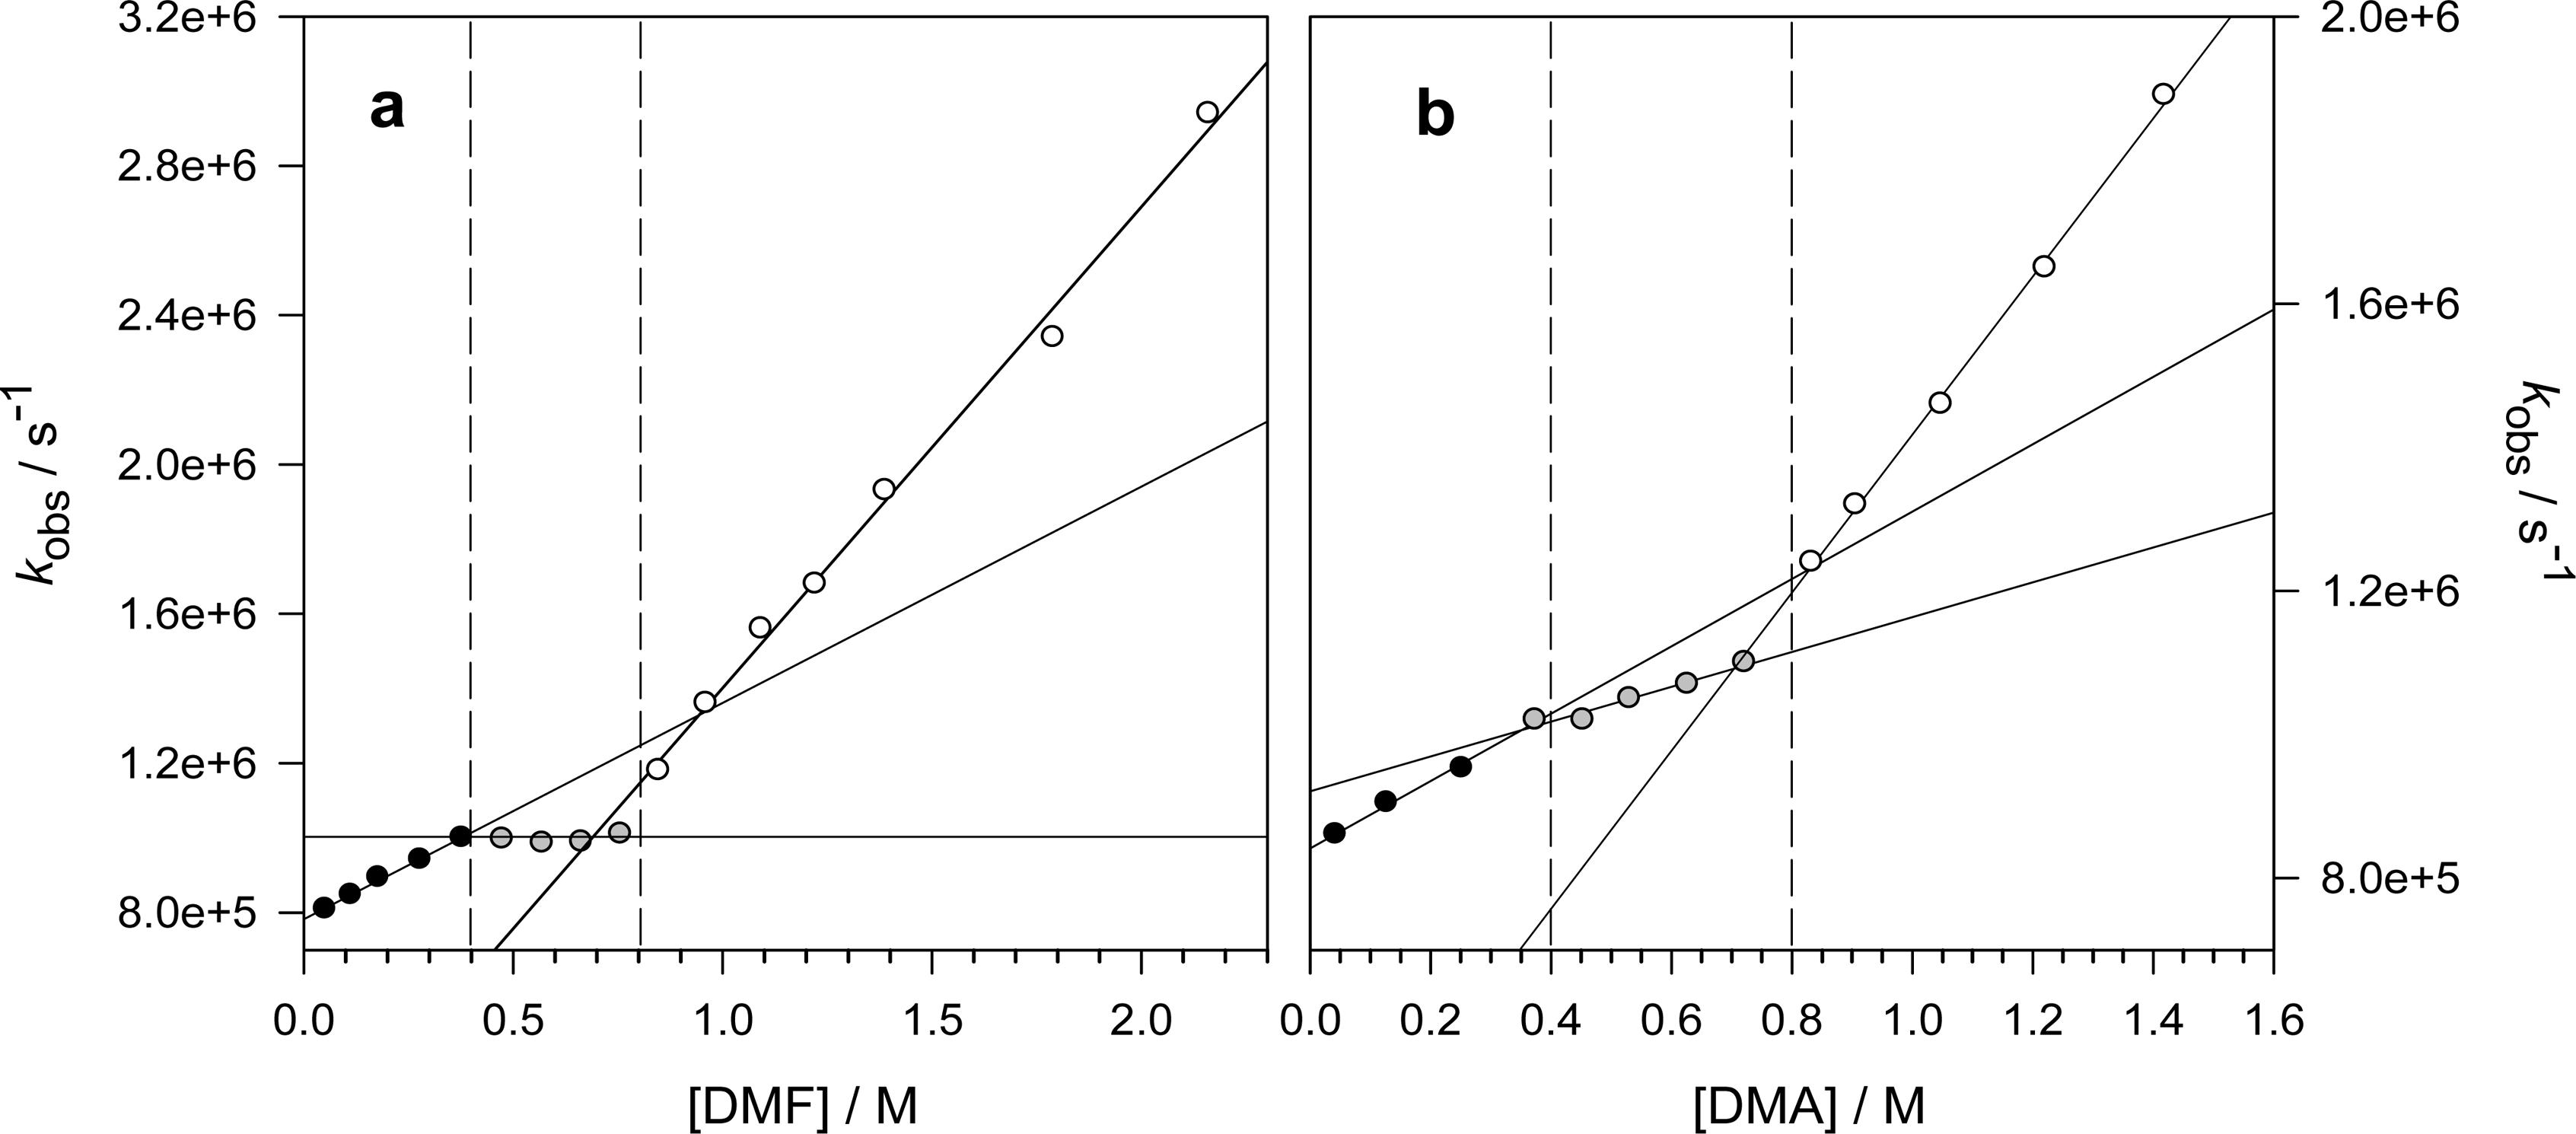
\includegraphics[width=\textwidth]{figures/kH-dma-dmf-mgclo42.png}
  \caption[Plot of observed rate constant against concentration of DMF and DMA
  for reaction with \cumo\ at 298 K in the presence of 0.2 M \ch{Mg(ClO4)2}.]
  {\textbf{a)} Plot of observed rate constant against concentration of DMF for
	  reaction with \cumo\ at 298 K in the presence of 0.2 M
	  \ch{Mg(ClO4)2}. 0--0.4 M [DMF] range (black circles), $k_{H1}$ =
	  5.8\E{5} \Ms; 0.8--2.2 M [DMF] range (white circles), $k_{H2}$ =
	  1.3\E{6} \Ms.  \textbf{b)} Plot of observed rate constant against
  concentration of DMA for reaction with \cumo\ at 298 K in the presence of 0.2
  M \ch{Mg(ClO4)2}. 0--0.4 M [DMA] range (black circles), $k_{H1}$ = 4.7\E{5}
  \Ms; 0.4--0.8 M [DMA] range (grey circles), $k_{H2}$ = 2.4\E{5} \Ms; 0.8--2.2
  M [DMA] range (white circles), $k_{H3}$ = 1.1\E{6} \Ms. Reprinted with
  permission from Reference~\protect\citenum{Salamone2015metals}. Copyright
  2015 American Chemical Society.} \label{fig:k-metals-mg}
\end{figure}

The addition of both \ch{LiClO4} and \ch{LiOTf} decrease to a similar extent the
rate constants for abstraction from DMF and DMA by \cumo. However, in contrast
to \ch{Mg(ClO4)2}, the lithium salts strongly deactivate \ch{C-H} bonds for 2
equivalents, followed by weak deactivation for another 2 equivalents, and no
deactivation for [amide]/[\ch{Li^{+}}]$<$4. Salamone et al. were not able to
give a clear cut explanation, but suggest that the different patterns are a
result of differences in charge density, which is greater for \ch{Mg^{2+}} than
\ch{Li^+}, as well as different coordination geometries of the two ions. A
coordination number of 4 is most common for \ch{Li^+}, while an octahedral
geometry with the coordination of 6 ligands is almost always observed for
\ch{Mg^{2+}}.\cite{Babu2013, Dudev2014} As a result, interactions of the ions
with solvent and counter-anions were suggested to be more important for
\ch{Mg^{2+}} than \ch{Li^+}.

\ch{NaClO4} and \ch{Ca(ClO4)2} influence HAT between \cumo\ and DMA to different
extents than both \ch{LiClO4} and \ch{Mg(ClO4)2}. \ref{fig:k-metals-naca}a,b
shows the plots of $k_{obs}$ against [substrate] for the reactions of \cumo\
with DMA in MeCN containing 0.2 M \ch{NaClO4} and \ch{Mg(ClO4)2}, respectively.
For \ch{NaClO4}, an almost negligible deactivation of \ch{C-H} bonds is observed
for up to 4 equivalents of DMA. This was explained on the basis of the weaker
Lewis acidity of \ch{Na^+} as compared to \ch{Li^+}. With regards to
\ch{Ca(ClO4)2}, binding to DMA fully deactivates \ch{C-H} bond abstraction up to
4 equivalents of DMA. The first region of~\ref{fig:k-metals-naca}b ([DMA] =
0--0.2 M, black circles) represents the decrease in $k_\beta$ of \cumo\ as
\ch{Ca^{2+}} preferentially binds to DMA over \cumo. Interestingly, for both DMF
and DMA, the same experiments in dimethyl sulfoxide (DMSO) solvent show no
inhibition of HAT reactivity by metal cations. This was rationalized on the
basis of the stronger Lewis basicity of DMSO as compared to both MeCN and the
amides, thus the metals preferentially bind the solvent rather than amide
substrate.

\begin{figure}[!htbp]
  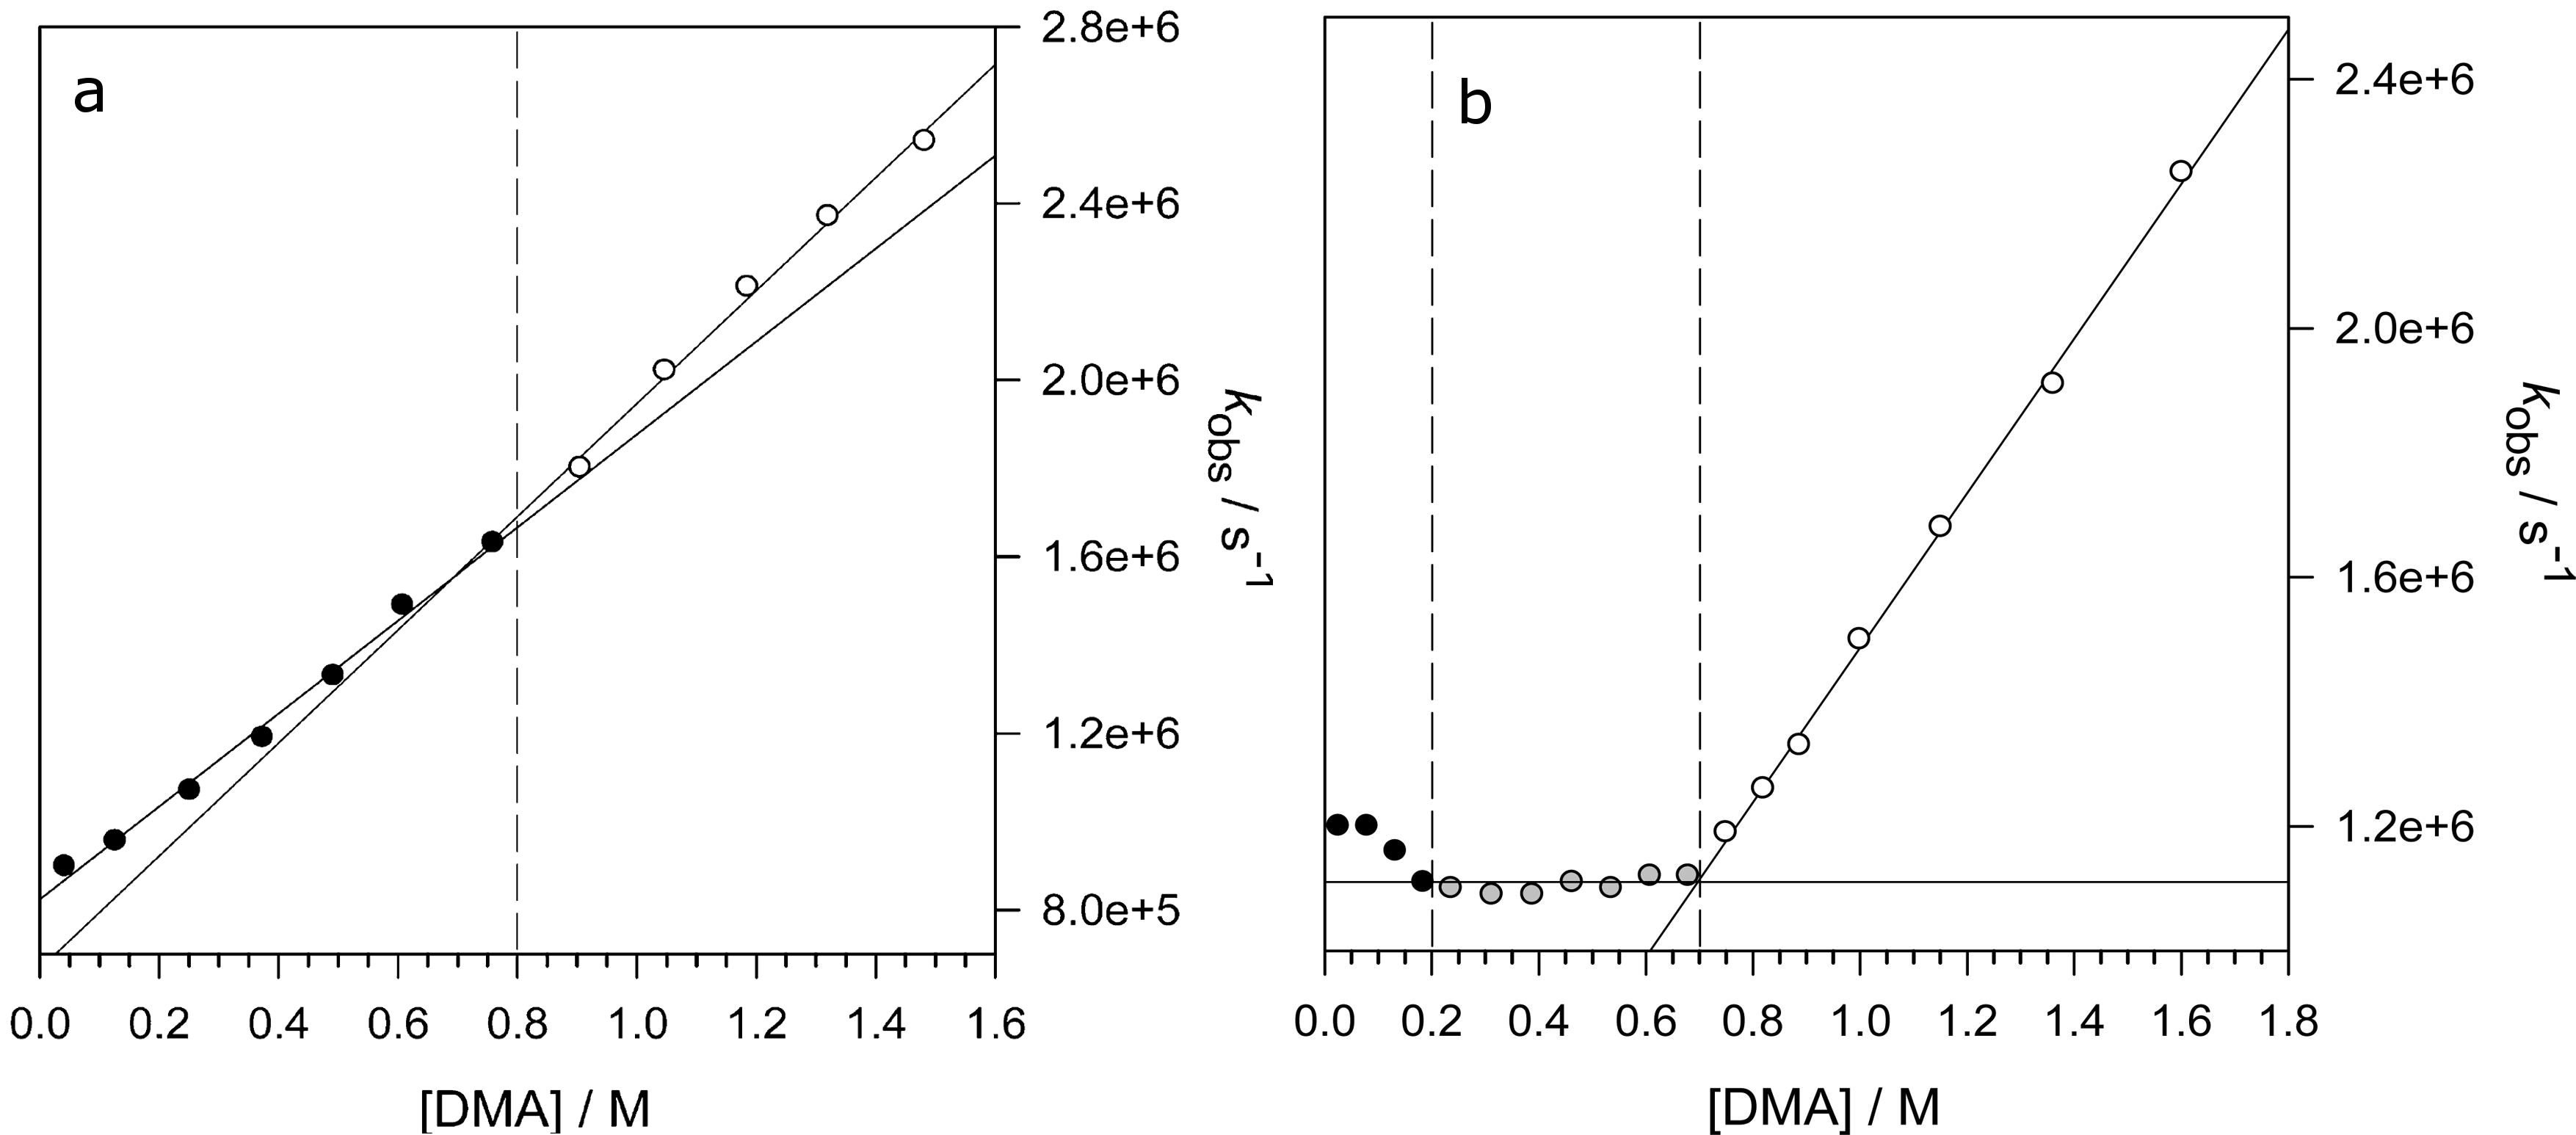
\includegraphics[width=\textwidth]{figures/exptdma-na-ca.png}
  \caption[Plot of observed rate constant against concentration of DMA for
  reaction with \cumo\ at 298 K in the presence of 0.2 M \ch{NaClO4} and
  \ch{Mg(ClO4)2}.] {\textbf{a)} Plot of observed rate constant against
	  concentration of DMA for reaction with \cumo\ at 298 K in the
	  presence of 0.2 M \ch{NaClO4}. 0--0.8 M [DMA] range (black circles),
	  $k_{H1}$ = 9.6\E{5} \Ms; 0.8--1.4 M [DMA] range (white circles),
	  $k_{H2}$ = 1.4\E{6} \Ms.  \textbf{b)} Plot of observed rate constant
  against concentration of DMA for reaction with \cumo\ at 298 K in the
  presence of 0.2 M \ch{Ca(ClO4)2}. 0.8--1.7 M [DMA] range (white circles),
  $k_{H1}$ = 1.2\E{6} \Ms. Adapted with permission from
  Reference~\protect\citenum{Salamone2015metals}. Copyright 2015 American
  Chemical Society.} \label{fig:k-metals-naca}
\end{figure}

Finally, \citet{Salamone2016} examined the effects of substrate structure on HAT
reaction between \cumo\ and sterically bulky tertiary alkanamides in the
presence of alkali and alkaline earth metal ions. For $N,N$-dialkylacetamides,
the steric bulk of the $N$-alkyl groups was previously
characterized.\cite{Salamone2014} Steric repulsion between \cumo\ and the
$N$-alkyl groups can decreases the HAT rate constant, as evident by the 3-fold
decrease in $k_H$ in going from DMA to $N,N$-diisobutylacetamide (DIA; 1.2\E{6}
and 3.1\E{5} \Ms, respectively). For reactions of \cumo\ with DIA addition of
0.2 M \ch{LiClO4} or \ch{Ca(ClO4)2} to results in the same trends in \ch{C-H}
bond deactivation observed for DMA. This indicates that the influence of metal
cation-substrate binding is not significantly influenced by the steric bulk of
$N$-alkyl groups.  The same is true for the addition of 0.2 M \ch{Mg(ClO4)2} to
abstraction from DIA by \cumo, as shown in~\ref{fig:k-dia-mg}. Once again, a
slight decrease in reactivity is observed for the first 2 equivalents of DIA,
followed by strong C-H bond deactivation for an additional two equivalents, and
no deactivation beyond that. No additional insight was provided by Salamone et
al. as to the reason for this reactivity. The plausible explanation provided was
once again that \ch{Mg^{2+}} has a high charge density. These results show that
Lewis acid-base interactions between alkali or alkaline earth metal cations can
greatly depress hydrogen abstraction by alkyoxyl radicals.

\begin{figure}[!htbp]
  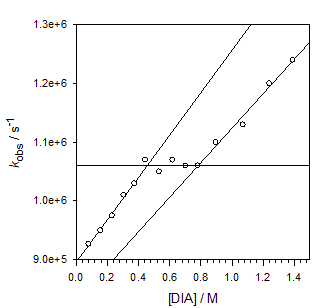
\includegraphics[width=0.6\textwidth]{figures/exptdia-mg.png}
  \caption[Plot of observed rate constant against concentration of DIA for
  reaction with \cumo\ at 298 K in the presence of 0.2 M \ch{Mg(ClO4)2}.]{Plot
	  of observed rate constant against concentration of DIA for reaction
	  with \cumo\ at 298 K in the presence of 0.2 M \ch{Mg(ClO4)2}. 0--0.4
	  M [DIA] range, $k_{H1}$ = 3.6\E{5} \Ms; 0.8--1.4 M [DIA] range,
	  $k_{H2}$ = 2.9\E{5} \Ms.  Reprinted from Tetrahedron, 72, Salamone et
  al., Hydrogen atom transfer from tertiary alkanamides to the cumyloxyl
  radical. The role of substrate structure on alkali and alkaline earth metal
  ion induced \ch{C–H} bond deactivation, 7757--7763, 2016, with permission
  from Elsevier.} \label{fig:k-dia-mg}
\end{figure}

With these results in mind, I am interested in the possibility that alkali and
alkaline earth metal cations found in biological system can protect \ch{C-H}
bonds in proteins from HAT to reactive oxygen-centred radicals. However, the
experimental results do not answer some of the key physico-chemical determinants
that may make this possible. Specifically, I have composed several important
research questions that remain unclear from the experimental results.

The first question I have is one of methodology: Can DFT-based methods can
accurately treat alkali/alkaline metal cation binding to organic substrates or
radicals? There exists limited ab initio data describing these
interactions.\cite{ Siu2001, Corral2003, Suarez2011, Baldauf2013} Therefore, I
have conducted a benchmark quality study involving \ch{Li^+}, \ch{Na^+},
\ch{Mg^{2+}}, \ch{K^+}, and \ch{Ca^{2+}}. To the best of my knowledge, this
represents the first systematic benchmark study of these metal cations with both
organic substrates and radicals.

Secondly, the nature of the binding of metal ions to substrates is still poorly
described, especially given the odd stoichiometric effects observed for
\ch{Mg(ClO4)2} with alkylamides. Specifically, I wish to address the range of
these interactions, and how much the metals effect the C-H being broken. To
address this I have utilized both \ch{Na^+} and \ch{Mg^{2+}} in my calculations.
These metal ions were chosen to capture the large differences in Lewis acidity
and ion size associated with these third-period ions, and because they are two
of the most biologically relevant metal ions.

Thirdly, I address the effect that metal ions have on the HAT barrier heights.
Experiments demonstrate that under certain conditions, the presence of metal
ions can decrease HAT reactivity. If metal ions do effectively increase C-H bond
strengths, this will be a contributing factor to the free energy barrier as per
the BEP principle\cite{Bell1936,Evans1938} (see Chapter~\ref{ch:bde}). There
will likely be additional factors such as polarization in the TS complex, or
other effects of possible charge transfer from the substrate to metal ions (or
vice versa). To investigate this, I have primarily studied HAT reactions
involving DMA and oxygen-centred radicals. Given there are only experimental
data for \cumo, this is the primary subject, however I was interested in
structural differences of the oxygen-centred radical, thus I have utilized \bno\
as well, which differs significantly in that it has the ability to form strong
pre-reaction complexes with hydrogen bond accepting
substrates.\cite{Salamone2012, Salamone2013} I also investigated the effect
metal cations have on the abstraction from DMA by the more biologically relevant
hydroxyl radical. I have also performed calculations with the bulkier DIA
substrate and \cumo\ to verify whether or not steric bulk does have an influence
on the ability of a metal cation to affect HAT reactions.

Finally, given that reactions of DMA with \cumo\ in the presence of metal salts
show no deactivation, I was interested in studying the reactivity of alkoxyl
radicals with strong Lewis bases. Strong Lewis basic compounds are important as
they are often used as solvents in physical organic chemical experiments.
Furthermore, strong Lewis acids are common in biological systems. Specifically,
phosphates represent an important functionality as part of the DNA backbone, as
well being important in adenosine triphosphate (ATP), the so-called ``energy
currency.'' Sulphur containing amino acids are also susceptible to oxidation
into sulfoxides and disulfoxides.\cite{Lee2009} Therefore,
understanding the HAT reactivity of strong Lewis basic compounds with
oxygen-centred radicals also contributes to the understanding of oxidative
stress in biological systems.

HAT reactions involving alkoxyl radicals and strong Lewis bases have been
previously studied,\cite{Salamone2012, vanSanten2016} and can possess
interesting and unusual chemical reactivity. For instance, we recently showed
that for the HAT reaction between \bno\ and DMSO, \bno\ acts as a hydrogen atom
donor rather the acceptor.\cite{vanSanten2016} In light of this, I examined the
effect of metal cations on the expected HAT reactivity between \cumo\ and DMSO,
as well as the radical H-atom donation reactivity between \bno\ and DMSO. I also
performed calculations to determine the effects of metal cations and if there
exists reverse reactivity for two other strong Lewis basic substrates:
hexamethylphosphoramide (HMPA) and tributylphosphine oxide (TBPO). These results
are reported in~\ref{ap:hat}. The chemical structures of all the species studies
herein are shown in~\ref{fig:hat-subs}.

\begin{scheme}[!htbp]
  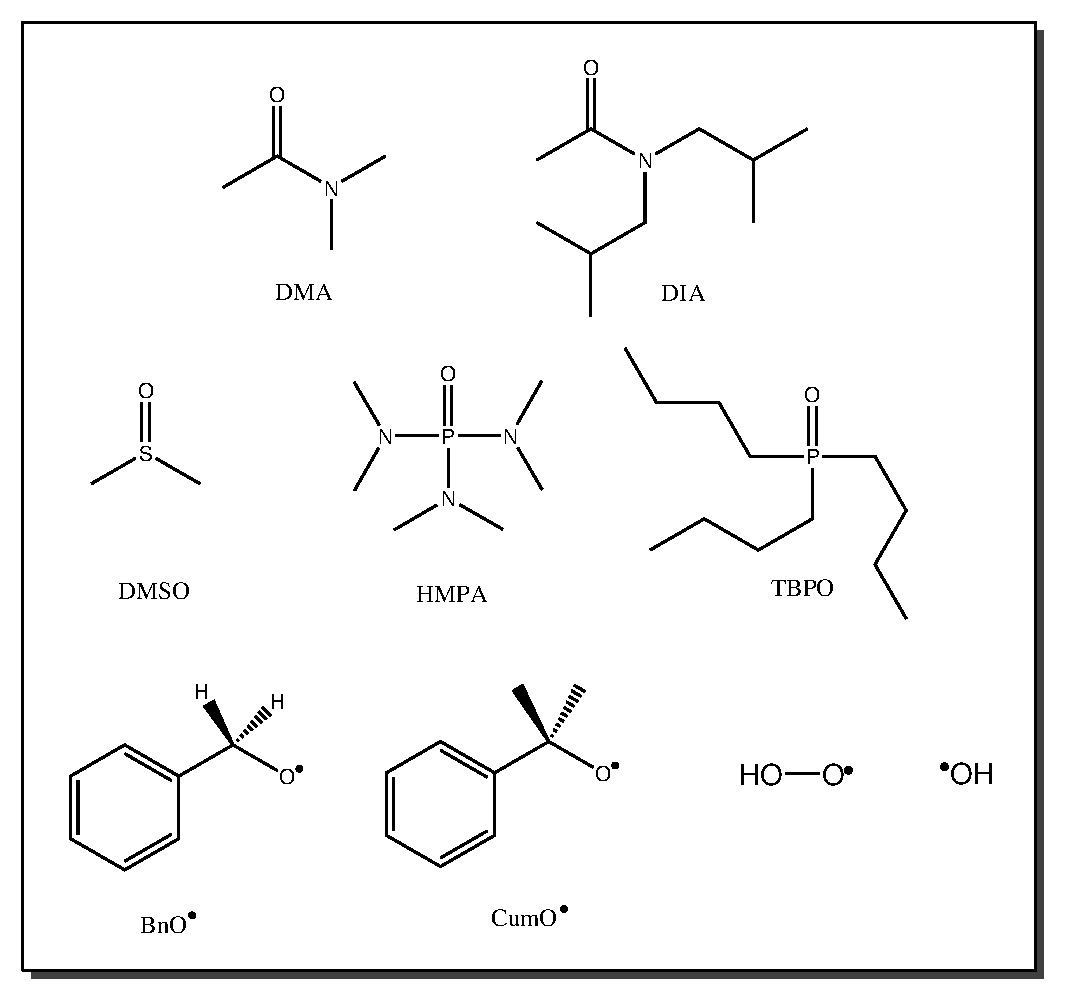
\includegraphics[width=\textwidth]{figures/Substrates.eps}
  \caption{Chemical structures of the species studies herein.}
  \label{fig:hat-subs}
\end{scheme}


\section{Computational methods and details}

All quantum mechanical calculations were performed using either the Gaussian 09
software package,\cite{Frisch2009} or the TURBOMOLE software
package.\cite{turbomole} Detailed benchmark studies of metal cation-substrate
interactions were carried out, the full data and discussion of which is
presented in Appendix~\ref{ap:hat}. Calculations for the benchmark quality data
of metal binding to substrates were first optimized at the
LC-$\omega$PBE-D3(BJ)/6-31+G(2d,2p) level of theory,\cite{Vydrov2006,
Vydrov2006a, Grimme2010, Johnson2006} and later re-optimized with larger
6-311+G(3df,3pd) basis sets. Single-point energy calculations were then carried
out using the coupled cluster methodology with single, double and perturbative
triples with full core correlation, CCSD(T,Full), and various basis sets. Final
benchmark quality binding energies have been calculated using the F12$^*$
explicitly correlated method with Def2-QZVPPD primary basis sets and Def2-QZVPP
auxiliary basis sets required for the resolution-of-the-identity (RI)
approximation as implemented in TURBOMOLE. The RI approximation is used to
reduce the computational cost associated with calculating MO
integrals.\bibnote{For a detail description of the RI approximation and explicit
correlation, see Ref.~\protect\citenum{OterodelaRoza2017}, Chapter 4.} A total
of 31 different DFT-based methods with nearly complete 6-311+G(3df,3pd) and
moderate sized 6-31+G(2d,2p) basis sets were tested both by single-point energy
calculations on the LC-$\omega$PBE-D3(BJ)/6-311+G(3df,3pd) optimized reference
structures. Geometry optimization calculations starting from the reference
structures were also performed for three of the best performing DFT-based
method, in order to verify their ability to capture the minimum energy bound
structures. The final DFT-based method selected from this benchmark work is
M05-2X.\cite{Zhao2006}

To test the effects of metal cations on HAT barrier heights, calculations were
first performed for the reactions not involving metal cations. Geometry
optimizations were performed at the M05-2X/6-31+G$^{**}$ level of
theory. Transition state (TS) structures were obtained by first freezing the
abstraction donor-hydrogen-acceptor bond lengths with multiple initial
orientations. The frozen bonds were then relaxed to obtain the final TS
structures, which were then used to identify the appropriate pre- and
post-reaction complexes. All structures were subjected to harmonic vibrational
frequency calculations, which were visualized using the Chemcraft
program\cite{ccraft} to verify minima (or saddle-points with a single imaginary
frequency connecting reactants to products for TS structures). Single-point
energy calculations were performed at the M05-2X/6-311+G(2d,2p) level of theory.
The effects of MeCN solvent were estimated by inclusion of the
SMD\cite{Marenich2009} continuum solvent model in single-point energy
calculations.

The inclusion of metal cations into the TS structures proved to be technically
challenging. It was my expectation that I could simply include metal cations and
necessary counter-anions into the minimum energy complex structures and
re-optimize, however this was not the case. TS structures were once again
obtained by constrained optimization with the inclusion of the metal cation and
counter-anion and freezing the abstraction donor-hydrogen-acceptor bond lengths,
providing a guess TS structure. However, in most cases the force constants
(which are necessary for a TS optimization calculation) from the guess TS
structure were not representative of the true TS structure, thus force constants
were recalculated for every step along the optimization, using the ``CalcAll''
keyword in Gaussian. This is a very computationally expensive procedure. Even
using this method, many TS structures including metal cations failed to
converge. Therefore, guess TS structures that contain a single imaginary
frequency connecting reactants to products are used in place. This technique
provides genuine TS structures, although they may not be the TS associated with
the minimum energy reaction pathway. Nonetheless, the guess TS structure can be
used provide an estimate of the reaction barrier height that are verified with
calculations that were successful. Where available, final TS structures were
used to identify the appropriate pre- and post-reaction complexes.

Natural bond order (NBO) and natural population analysis (NPA) were utilized in
order to investigate the electronic structures involved in the HAT reactions and
the effects of metal cation binding.\cite{Reed1983, Reed1985, Glendening2012}
Version 3.1 of the NBO software package,\cite{NBO3} as implemented in the
Gaussian 09 package was used in all cases.\cite{Frisch2009} NBO analysis
provides a means for estimating the physical effects of chemically intuitive
orbital interactions while NPA charges are a means for calculating the
occupancies and charges of atomic centres.\cite{Landis2014, Weinhold2016}

\section{Exploring the nature of metal cation substrate interactions}

The first step to understanding the effect non-redox active metal have on HAT
reaction barrier heights is investigating the nature of the binding interaction.
\ref{fig:pes-dma-na}a,b show the potential energy surfaces (PESs) of the binding
of sodium ion, and sodium chloride to DMA, respectively. There are three
surfaces in each plot representing the same potential energy surface in the
gas-phase (black circles), and in an SMD\cite{Marenich2009} continuum solvent
field of MeCN (grey squares) or water (white circles). For both sodium ion and
sodium chloride, the gas-phase PES demonstrates strong binding with respect to a
solvated system. This is indicated by a much deeper well than both solvents and
a long-range interaction that does not tail off within 6 \AA\ due to the lack of
screening. This underscores the importance of including solvent effects in
studying the effects of metal cations. Interestingly, for the effects of water
compared to MeCN solvent appears to be quite small. In both cases the difference
between the minimum of the water PES is about 2.5 \kcalmol. Furthermore, the
minimum of the PES well in all cases falls at about the same distance (2.1--2.2
\AA) in the gas-phase and in both solvents. The small differences in binding
interactions indicate that the effects as measured in MeCN may also apply to the
more biologically relevant aqueous system.

For both the ion and the salt of sodium in water and MeCN, the binding
interaction only approaches zero slowly. Even at 6 \AA, the predicted binding
energy of DMA in water with \ch{Na^+} and \ch{NaCl} are 1.1 and 0.7 \kcalmol,
respectively. This is an indication that M05-2X-SMD does not properly capture
long-range interactions of DMA with sodium. This may be a result of not fully
capturing the screening effect of solvent. Nonetheless, at a distance of 5 \AA,
which corresponds well with the size of the first solvation shell of the sodium
ion,\cite{Degreve1996} the interaction between DMA and sodium is nearly zero.
This result is consistent with literature that studies the Hofmeister series,
where it has been shown that biologically relevant cations are only able to
influence their immediate solvation shell.\cite{Omta2003, Funkner2011}
Furthermore, \citet{Heyda2009} utilized molecular dynamics simulations of
$N$-methylacetamide in aqueous solutions of NaCl, NaBr, KCl, and KBr to obtained
radial distribution functions (RDFs). The RDFS are in agreement with the
calculated PESs in that the most probable distance to find \ch{Na^+} from the
amidic oxygen-centre is at about 2--2.5 \AA\ separation. Heyda et al. also
showed that \ch{Na^+} binds more strongly with the amide than \ch{K^+}, and that
the nature of the halide counteranion does not contribute significantly to the
overall interaction. This is consistent with the results of Salamone et al.,
which showed that the nature of the counteranion plays a negligible role to the
effect on rate constants.\cite{Salamone2013a} The calculated binding energies of
\ch{NaCl} and \ch{NaClO4} to DMA are very similar in magnitude (16.0 and 18.1
\kcalmol, respectively). From these results it is possible to draw an important
conclusion: The use of \ch{Cl^-} in the calculations may reasonably reflect the
trends observed by Salamone et al.  with \ch{ClO4^-} and \ch{OTf^-}.

\begin{figure}[!htbp]
\centering
\vspace{1.0cm}
\hspace*{-1.2cm}
\begin{minipage}{8cm}
  \centering
  \begin{overpic}[width=\textwidth]{figures/pes_dma_na}
  \put(5,70) {\large\textbf{a.}}
\end{overpic}
\end{minipage}%
\begin{minipage}{8cm}
  \centering
  \begin{overpic}[width=\textwidth]{figures/pes_dma_nacl}
  \put(5,70) {\large\textbf{b.}}
\end{overpic}
\end{minipage}
\caption[Potential energy surface of binding energy between DMA and sodium
cation and sodium chloride.]{Potential energy surface of binding energy between
DMA and \textbf{a)} sodium cation and \textbf{b)} sodium chloride as a function
of O-Na interaction distance (\AA). The black line and points represent
gas-phase results, the grey squares and line is in continuum MeCN solvent, and
white circles and dashed line is in continuum water solvent. Calculated as a
rigid scan from the M05-2X/6-31+G$^{**}$ minimized complex structure at the
M05-2X/6-311+G(2d,2p) level of theory with the SMD solvent model.}
\label{fig:pes-dma-na}
\end{figure}

\ref{fig:pes-dma-mg}a,b show the PESs of the binding of magnesium ion, and
magnesium dichloride to DMA, respectively. As is the case for \ch{Na^+}, the
gas-phase PES of \ch{Mg^{2+}} is very strongly bound. In fact, the binding
energy does not asymptotically approach zero. At an O--Mg distance of 12 \AA,
there is calculated binding interaction of -48.5 \kcalmol, which is actually
greater than at 6 \AA\ by about 5 \kcalmol. This is a result of the the
ionization potentials (IP) of the metals with respect to that of DMA. The
experimental IP\cite{Slifkin1967, Baldwin1977, CRC2016} of DMA is 8.8--9.2 eV,
the first IP of Na is 5.1 eV, and the second IP of Mg is 15.0 eV (calculated
with M05-2X/6-311+G(2d,2p) = 8.9, 5.0, and 14.9 eV, respectively). In a solvated
system, magnesium ions exist invariably in the +2 oxidation state, however, due
to nature of the IPs, DFT-based methods prefer to transfer charge, resulting in
a non-convergent binding interaction between DMA and \ch{Mg^2+}, but not for
\ch{Na+}.

\begin{figure}[!htbp]
\centering
\vspace{1.0cm}
\hspace*{-1.2cm}
\begin{minipage}{8cm}
  \centering
  \begin{overpic}[width=\textwidth]{figures/pes_dma_mg}
  \put(5,70) {\large\textbf{a.}}
\end{overpic}
\end{minipage}%
\begin{minipage}{8cm}
  \centering
  \begin{overpic}[width=\textwidth]{figures/pes_dma_mgcl2}
  \put(5,70) {\large\textbf{b.}}
\end{overpic}
\end{minipage}
\caption[Potential energy surface of binding energy between DMA and magnesium
cation and magnesium chloride.]{Potential energy surface of binding energy
between DMA and \textbf{a)} magnesium cation and \textbf{b)} magnesium chloride
as a function of O-Mg interaction distance (\AA). The black line and points
represent gas-phase results, the grey squares and line is in continuum MeCN
solvent, and white circles and dashed line is in continuum water solvent.
Calculated as a rigid scan from the M05-2X/6-31+G$^{**}$ minimized complex
structure at the M05-2X/6-311+G(2d,2p) level of theory with the SMD solvent
model.} \label{fig:pes-dma-mg}
\end{figure}

The inclusion of MeCN and water solvent appear at first glance to alleviate this
problem. Note however that both PESs cross over zero binding at about 3
\kcalmol, indicating there is still charge transfer to some extent.
Additionally, for magnesium chloride in the gas-phase, there also appears to be
charge transfer occurring, as evident by the PES crossing zero just below 4
\kcalmol. On the other hand, the inclusion of either water or MeCN solvent with
\ch{MgCl2} give reasonable PESs with a binding interaction of about 25 \kcalmol\
for both water and MeCN, and a tailing off at about 3 \AA, or slightly larger
than the size of the first hydration shell of \ch{Mg^2+} (ca. 2
\AA).\cite{Chatterjee2013} Therefore, studying the effects of magnesium on HAT
reaction barrier may be possible using \ch{MgCl2}, however given the
difficulties with Mg in general, I elected to focus only on \ch{NaCl} for future
considerations.

Next, I performed calculations to determine if the interaction of metal cations
systematically increase the bond strengths of \ch{C-H} bonds in the models of
interest in this work. This effect is hypothesized to occur due to a decrease in
electron density in the \ch{C-H} $\sigma^*$ orbital, which is normally present
due to hyperconjugative overlap. The BDEs for several substrates in the presence
of \ch{Na^+} and \ch{NaCl} are listed in~\ref{tab:bde-metal}. The ROCBS-QB3 BDEs
for each of the substrates is included to demonstrate that the relative order of
BDEs for substrates with multiple \ch{C-H} bonds is reasonable. The BDE for an
arbitrary metal substrate complex (\ch{M\bond{dotted}X-H}) can be calculated as:

\begin{equation}
BDE = E(\ch{M\bond{dotted}X^.}) + E(\ch{H^.}) - E(\ch{M\bond{dotted}X-H})
\end{equation}

\begin{table}[!htbp]
  \caption[Bond dissociation enthalpies of DMA, DMSO, MeCN, and DIA with and
  without metal cations.]{Bond dissociation enthalpies of DMA, DMSO, MeCN, and
  DIA with \ch{Na^+}, \ch{NaCl}, and without metal cations (Bare) calculated at
  the M05-2X-SMD(MeCN)/6-311+G(2d,2p)//M05-2X/6-31+G$^{**}$ level of theory.
  ROCBS-QB3-SMD(MeCN) BDEs without metals are included for reference. All values
  are in \kcalmol.} \label{tab:bde-metal}
  \begin{tabular}{l c c c c}
                    & ROCBS-QB3 & \multicolumn{3}{c}{M05-2X} \\
                    \cline{2-5}
    Substrate       & Bare      &    Bare    &\ch{Na+}    &\ch{NaCl}   \\
    \hline
    DMA (acetyl)    & 101.0 & 98.5 & 97.8 & 98.4 \\
    DMA (cis)       & 94.8 & 92.2 & 93.2 & 94.0 \\
    DMA (trans)     & 94.3 & 91.6 & 92.8 & 92.6 \\
    DMSO            & 104.3 & 103.4 & 104.4 & 103.7 \\
    MeCN            & 99.0 & 97.4 & 98.3 & 98.1 \\
    DIA (acetyl)    & 99.7 & 97.8 & 97.5 & 97.7 \\
    DIA ($\alpha$-cis)  & 97.0 & 95.7 & 96.5 & 95.3 \\
    DIA ($\beta$-cis)   & 98.3 & 96.4 & 94.8 & 93.1 \\
    DIA ($\alpha$-trans)& 94.6 & 93.0 & 93.8 & 94.0 \\
    DIA ($\beta$-trans) & 97.3 & 95.3 & 95.5 & 95.5
  \end{tabular}
\end{table}

For DMA, the $N$-methyl groups cis and trans relative to the carbonyl are the
weakest, and therefore most thermodynamically favourable for abstraction.
\citet{Salamone2013} showed that both \bno\ and \cumo\ prefer to abstract from
the $N$-methyl groups of DMA, rather than the acetyl group. The complexation of
\ch{Na^+} increases the cis BDE by 1.0 \kcalmol\ and the trans BDE by 1.2
\kcalmol. The complexation of \ch{NaCl} to DMA increases the cis BDE by 1.8
\kcalmol\ and the trans BDE by 1.0 \kcalmol. One would expect the greater
positive charge of the sodium cation (as compared to the sodium moiety of
\ch{NaCl}) to have a greater effect on the BDEs, however these calculations
indicate this may not always be the case. Specifically, the cis BDE is 0.8
\kcalmol\ weaker for the \ch{DMA-NaCl} complex as compared to the \ch{DMA-Na^+}
complex. These results, which are inconsistent with the hypothesis, can be
explained by additional analysis of both the parent and radical complexes. The
structures of the DMA-NaCl complex and three possible radical complexes are
shown in~\ref{fig:dma-na-cl}a-d.

\begin{figure}[!htbp]
	\centering

	\subfigure[DMA-NaCl]{
		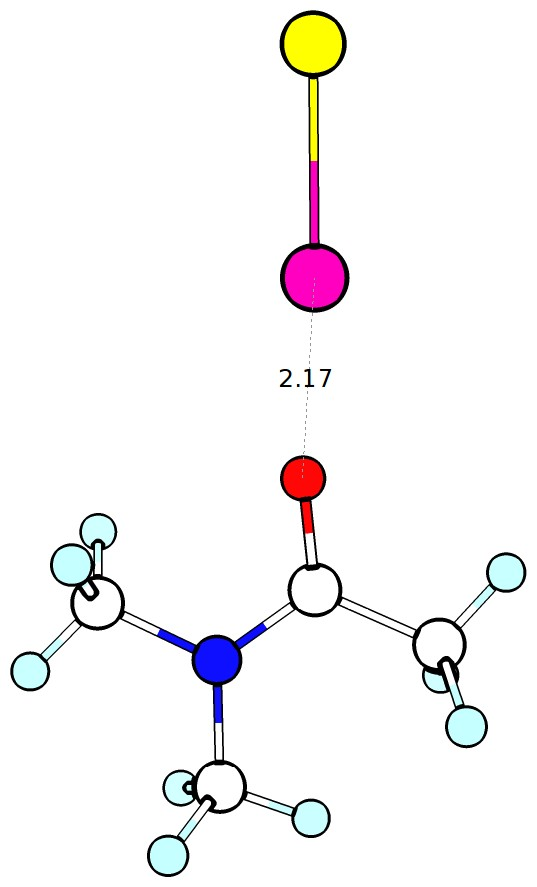
\includegraphics[width=4cm]{figures/dma-na-cl}
	}
  \subfigure[Acetyl radical]{
		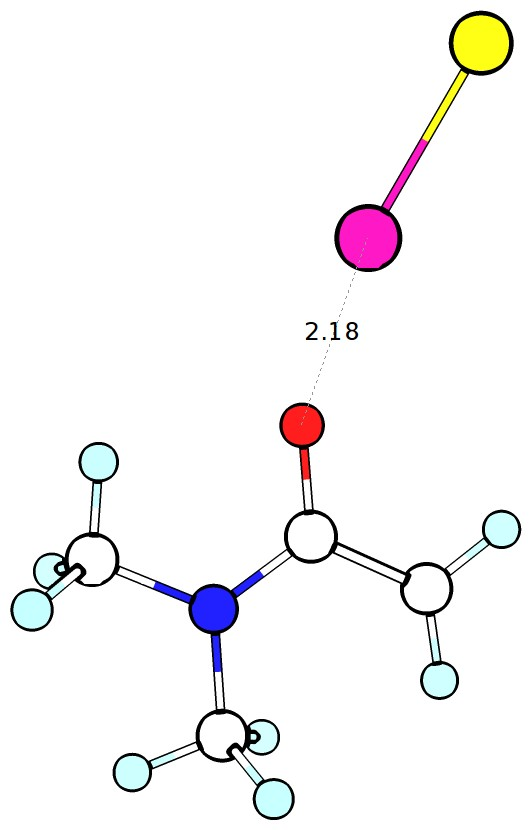
\includegraphics[width=4cm]{figures/dma-na-cl-acetyl}
	}
  \subfigure[Cis radical]{
    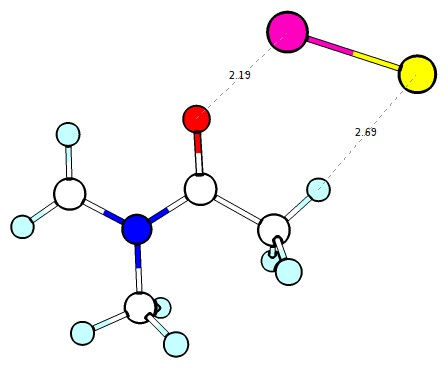
\includegraphics[width=6cm]{figures/dma-na-cl-cis}
  }
  \subfigure[Trans radical]{
    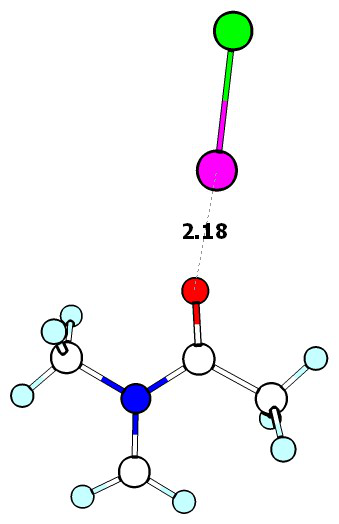
\includegraphics[width=4cm]{figures/dma-na-cl-trans}
  }

\caption[Structures of the DMA-NaCl complex and associated radical
complexes.]{Structures of \textbf{a} the DMA-NaCl complex, \textbf{b} the
DMA-NaCl acetyl radical complex, \textbf{c} the DMA-NaCl cis
radical complex, and \textbf{d} the DMA-NaCl trans radical complex. Key
interaction distances are shown in units of \AA. Element colour key: white is
carbon, light blue is hydrogen, red is oxygen, blue is nitrogen, purple is
sodium, and green is chlorine.} \label{fig:dma-na-cl}
\end{figure}

NBO analysis can be used that give a qualitative description based on
perturbation theory of the energy contribution of specific NBO orbital
interactions.\cite{Weinhold2016} Using NBO analysis on DMA, the estimated effect
of hyperconjugative overlap reveals a weakening of the $N$-methyl \ch{C-H} bonds
by approximately 5.6 and 5.9 \kcalmol\ for the cis and trans positions,
respectively. Upon complexation of \ch{Na^+}, the bond weakening effects become
3.7 and 4.1 \kcalmol\ for the cis and trans positions, respectively. Therefore,
from an NBO perspective, the cis an trans $N$-methyl bond strengths can be
described as strengthening upon complexation of \ch{Na^+}. Furthermore, the
predicted effect of hyperconjugative overlap in the \ch{DMA-NaCl} complex are
5.4 and 5.5 \kcalmol\ for the cis and trans positions, respectively. Again, from
an NBO perspective, the complexation of \ch{NaCl} can be said to strengthen the
$N$-methyl \ch{C-H} bonds in DMA, but not as much as \ch{Na^+}. NBO analysis of
the parent complexes thus supports the hypothesis.

However, BDEs can be affected by both parent and radical stability. The
hypothesis considers only the stability of the parent molecule, where
complexation of a metal-cation stabilizes the parent by withdrawing electron
density from an anti-bonding orbital. In the case of complexation of \ch{NaCl},
secondary interactions between the Cl moiety of \ch{NaCl} and the radical can
result in the destabilization of the radical complex and a further increase in
the predicted \ch{C-H} BDE. This is the case for the cis-DMA-NaCl radical
complex (\ref{fig:dma-na-cl}c). The Cl moiety of \ch{NaCl} is attracted to the
partial positive charge of the acetyl hydrogen of DMA, which is greater than the
partial charge on the cis $N$-methyl hydrogens (0.25 $e^-$ vs. 0.21 $e^-$). This
leads to the donation of electron density from Cl to the \ch{C-H} $\sigma^*$
orbital. NBO estimates this orbital interaction to amount to about 1 \kcalmol of
bond weakening. Therefore, the hypothesis is incomplete in that it does not
account for radical complex stability. Furthermore, with respect to TS
complexes, additional interactions may further complicate the picture.

Interestingly, the predicted BDE for the acetyl position of DMA decreases,
rather than increasing as hypothesized, with both \ch{Na^+} and \ch{NaCl}. This
can be attributed to the change in electronic structure associated with the
complex. Consider the two possible resonance forms of DMA shown in
~\ref{fig:dma-res}. Glendening and Hrabal\cite{Hrabal1997} utilized natural
resonance theory to estimate that the right-hand resonance structure in the
closely related formamide contributes about 30\% to the overall resonance
hybrid. On the other hand, NBO analysis predicts a bond order in DMA of 1.5
between the C and O and the C and N. Nonetheless, the complexation of DMA to
\ch{Na^+} slightly increases the contribution of the zwitterionic form,
resulting in a decrease in electron density at the carbonyl carbon. This is
evidenced by the increase in NPA charge at the carbonyl carbon from +0.72 in DMA
to +0.74 in the DMA-\ch{Na^+} complex. The partially positively-charged carbon
centre inductively withdraws electron density, stabilizing the acetyl radical,
increasing the $\pi$-bonding character between the two carbon centres, and
decreasing the effective BDE.

The observed inductive effects also manifests in the decrease in the
carbonyl-acetyl C-C bond lengths in the acetyl radical, which decrease from
1.457 \AA\ to 1.443 \AA\ upon complexation of \ch{Na^+}. Complexation of
\ch{NaCl} results in a bond length of 1.451 \AA. These results are consistent
with the ordering of the calculated acetyl BDEs (DMA \textgreater\ \ch{DMA-NaCl}
\textgreater\ \ch{DMA-Na^+}). On the other hand, the amidic nitrogen becomes net
more positive upon complexation of either \ch{Na^+} or \ch{NaCl}, but still has
an NPA charge that is negative. As a results, there is no inductive
stabilization effect for the $N$-methyl radical complexes.

\begin{figure}[!htpb]
  \centering
  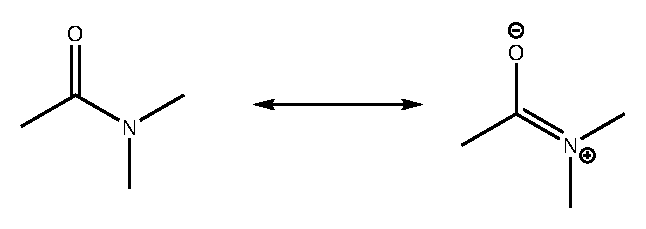
\includegraphics[width=0.7\textwidth]{figures/DMA-resonance.eps}
  \caption{The resonance forms of DMA.}
  \label{fig:dma-res}
\end{figure}

For MeCN and DMSO the complexation of either \ch{Na^+} or \ch{NaCl} results in
an increase in \ch{C-H} BDE.\@ In MeCN, the electron density in the \ch{C-H}
$\sigma^*$ anti-bonding orbital decreases as a result of the interaction between
\ch{Na} and the nitrogen centre. DMSO has a non-Lewis electronic structure,
making it difficult to analyze orbital interactions of valence-bond orbitals.
Nonetheless, there is normally hyperconjugative overlap between the sulphur
centre and the \ch{C-H} $\sigma^*$ anti-bonding orbitals, which was confirmed by
NBO analysis. The electron density in the \ch{C-H} $\sigma^*$ orbital decreases
as a result of the interaction of \ch{Na^+} with the oxygen-centre of DMSO.

Upon complexation of \ch{NaCl}, the BDEs of the more sterically bulky amide
substrate DIA follow the same trend that is observed as for DMA: The acetyl
\ch{C-H} BDE decreases due to inductive stabilization, while the \ch{C-H} bonds
$\alpha$ to the amidic nitrogen centre increase as a result of decreased
\ch{C-H} $\sigma^*$ occupancy. Alkoxyl radicals are not expected to abstract
from \ch{C-H} BDEs of the bonds $\beta$ to the nitrogen centre in DIA or other
longer chain $N$-alkyl amides, as the incipient radical is not stabilized by
amidic $\pi$-system. However, due to steric repulsion, the $\alpha$-radicals of
DIA cannot lie directly plane of allowing conjugation with the $\pi$-system. As
such the $\alpha$-\ch{C-H} BDEs of DIA are greater than those of DMA by 2-3
\kcalmol, and are closer to the $\beta$-\ch{C-H} BDEs than perhaps expected. The
effects of sodium binding to the amidic oxygen are almost nil for the
$\beta$-trans C-H bond of DIA, however there is a significant decrease in the
$\beta$-cis \ch{C-H} BDE. \ref{fig:dia-na-cl}a,b shows the structures of the
DIA-NaCl complex and the $\beta$-cis radical complex, where it can seen that the
metal cation interacts with both the oxygen-centre and the carbon-centred
radical. This interaction stabilizes the radical complex and thus decreases the
effective BDE, however this interaction is likely not possible in the TS
structure and is not expected to contribute to a reduction of the barrier
height.

\begin{figure}[!htbp]
	\centering

	\subfigure[DIA-NaCl]{
		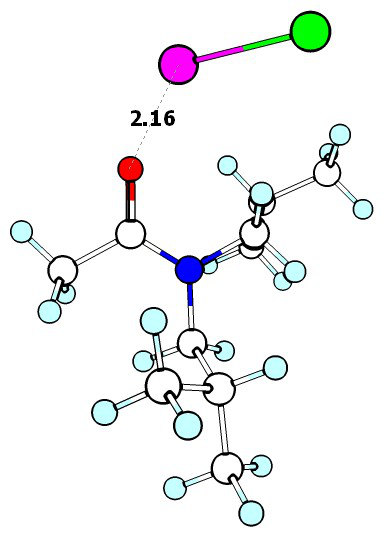
\includegraphics[width=5cm]{figures/dia-na-cl}
	}
  \subfigure[$\beta$-cis radical]{
		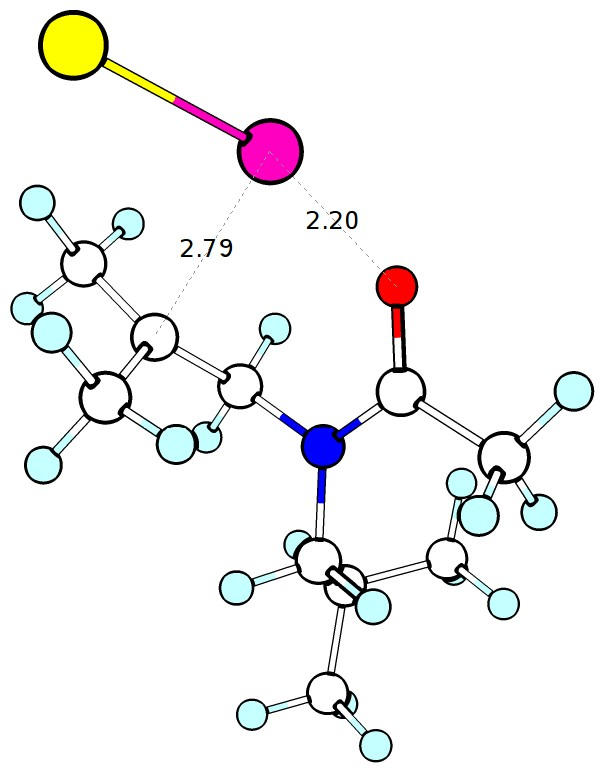
\includegraphics[width=5cm]{figures/dia-na-cl-rad-b}
	}

  \caption[Structures of the DIA-NaCl complex and radical complex.]{Structures
  of \textbf{a} the DMA-NaCl complex, \textbf{b} the DIA-NaCl $\beta$-cis
  radical complex. Key interaction distances are shown in units of \AA. Element
  colour key: white is carbon, light blue is hydrogen, red is oxygen, blue is
  nitrogen, purple is sodium, and green is chlorine.} \label{fig:dia-na-cl}
\end{figure}

All of these results together confirm that specific metal-substrate interactions
can increase the effective BDEs of abstractable \ch{C-H} bonds by decreasing
\ch{C-H} $\sigma^*$ occupancy. However, this is complicated by the possibility
for secondary interactions between the metal or counter-anion with the formed
radicals. Furthermore, additional factors such as induction can alter the
effects. It appears that for \ch{C-H} bonds $\alpha$ to atoms with LPs that
hyperconjugatively overlap with the \ch{C-H} $\sigma^*$ anti-bonding orbital,
the complexation of non-redox active metals increases the \ch{C-H} bond
strength. However, if the \ch{C-H} bond is adjacent to an electron-poor centre,
such as the carbon of a carbonyl, metal complexation actually decreases the bond
strength slightly by stabilizing the carbon-centred radical. In the context of
HAT reaction barrier heights, increasing the effective \ch{C-H} bond strength
should decrease the reaction-rate slightly by destabilizing the TS complex.
However, there are other important factors to consider such as how the metal
effects the dipole moment in the TS complex. Furthermore, it is important to
note that experiments showed that \ch{NaClO4} did not significantly effect the
HAT rate constants for reactions between \cumo\ and organic substrates.
Therefore, the effects observed herein likely are an exaggeration of what is
truly occurring in situ. Nonetheless, these theoretical calculations may be
useful in developing an understanding of the subtle nature of the effects of
non-redox active metal cations on HAT reactions in general.

With regards to the implications these results have on protein systems, since
abstraction occurs predominantly from an $\alpha$-\ch{C-H} bonds, it is likely
that the nature of the amino acid, and the three dimensional structure of the
protein will have significant importance. As the geometry of the peptide
backbone becomes more strained by steric interactions, the \$ch{C-H}
bond$\alpha$ hydrogen will become more difficult to abstract, as might be
exemplified by the higher \ch{C-H} BDEs in DIA as compared to DMA. In the
absence of secondary interactions, alkali or alkaline earth-metals are able to
bind to a given carbonyl site on the surface of a protein, they may exert a
chemo-protective effect by increasing the BDE of an adjacent \ch{C-H} bond.
However, the complexity of biological systems makes the absence of secondary
interaction unlikely. Therefore, the possibility for chemo-protection to occur
is remote.

\section{HAT reactions involving non-redox active metals}

\subsection{DMA}

Hydrogen abstraction reactions involving the oxygen-centred radicals \bno\ and
\cumo\ and DMA in MeCN have been previously investigated experimentally and
theoretically.\cite{Salamone2013} The HAT reaction between DMA and \bno\ was
determined to occur predominantly through a direct HAT mechanism from the
$N$-methyl group cis relative to the carbonyl, and is kinetically limited by the
formation of a strong pre-reaction complex between the relatively acid
$\alpha$-C-H of \bno\ and the amidic oxygen centre. On the other hand, \cumo\
cannot form a strong hydrogen-bonding interaction, and thus forms a
non-specific dispersion-bound pre-reaction complexes. Abstraction by \cumo\
still takes place from one of the $N$-methyl groups, but the rate constant is 2
orders of magnitude less than for \bno. Recall that the inclusion of metal salts
in reactions of DMA with \cumo\ were previously
investigated.\cite{Salamone2015metals} On the basis of the exaggerated effects
observed in the changes in BDEs and the technical difficulties associated with
these studies, the goal of this work is not to reproduce experimental results,
but rather, develop insights into the possible changes that can occur as a
result of metal salt addition to HAT reactions.

Herein, I have calculated the reaction barrier heights for all three
abstractable positions of DMA for HAT reactions involving \cumo\ and \bno, both
with and without \ch{NaCl}. These data are summarized in~\ref{tab:DMA-dG}.
Perhaps alarmingly, the free energy barriers calculated at the
M05-2X-SMD(MeCN)/6-311+G(2d,2p)//M05-2X/6-31+G$^{**}$ are systematically higher
than those previously calculated by about 8.5 \kcalmol.\cite{Salamone2013} The
previously calculated results were in reasonable agreement with experimental
results. The reason for this discrepancy is unclear, given that M05-2X has
previously been used successfully to calculate accurate HAT rate
constants.\cite{Galano2013} Furthermore, the optimized minimum energy structures
from both methods do not differ significantly, with the exception of slightly
shorter abstracting \ch{C-H} partial bonds and slightly elongated \ch{O-H}
partial in the TS structures excluding \ch{NaCl} (ca. 0.03 to 0.05 \AA).
However, the relative ranking and differences in energies for the reaction
barrier heights for the different \ch{C-H} bonds are consistent with previous
results. Therefore, although these results cannot be used to predict rate
constants, they are useful for studying the change in barrier height due to the
addition of NaCl.

\begin{table}[!htbp]
\caption[Calculated free energy (enthalpy) barrier for direct HAT from different
\ch{C-H} bonds in DMA by \cumo\ and \bno, with and without
\ch{NaCl}.]{Calculated free energy (enthalpy) barrier ($\Delta G(H)^\ddagger$,
\kcalmol) for direct HAT from different \ch{C-H} bonds in DMA by \cumo\ and
\bno, with and without \ch{NaCl}. The change in barrier height ($\Delta \Delta
G(H)^\ddagger$) is calculated relative to the same abstraction site without the
inclusion of \ch{NaCl}. All barrier heights are relative to separated reactants
(or complexed DMA-NaCl) and were calculated at the
M05-2X-SMD(MeCN)/6-311+G(2d,2p)//M05-2X/6-31+G$^{**}$ level of theory.}
\label{tab:DMA-dG}
  \begin{tabular}{l l c c}
Reaction   & Abstraction Site &  $\Delta G(H)^\ddagger$ & $\Delta\Delta G(H)^\ddagger$ \\
\hline
DMA + \cumo   &  trans              &  17.3(3.4)           &              \\
              &  cis                &  17.5(3.8)           &              \\
              &  acetyl             &  21.6(7.5)           &              \\
DMA-NaCl + \cumo &  trans              &  20.3(3.7)        &    3.0(0.3)  \\
              &  cis                &  18.4(1.2)           &    0.9(-2.6) \\
              &  acetyl             &  21.0(4.3)           &   -0.6(-3.2) \\
DMA + \bno    &  trans              &  16.5(3.7)           &              \\
              &  cis                &  17.5(3.6)           &              \\
              &  acetyl             &  20.8(7.8)           &              \\
DMA-NaCl + \bno &  trans              &  18.6(1.7)         &    2.1(-2.0) \\
              &  cis                &  17.8(4.7)           &    0.3(1.1)  \\
              &  acetyl             &  22.0(4.7)           &    1.2(-3.1)
  \end{tabular}
\end{table}

Focussing first on the barrier heights for HAT between DMA and \cumo, the
results of complexation with \ch{NaCl} is variable. For each of the acetyl, cis,
and trans \ch{C-H} bond positions of DMA, there are three distinct effects upon
complexation of \ch{NaCl}. For the trans position, both the free energy and
enthalpic barriers increase, for the cis position the free energy barrier
increases and the enthalpic barrier decreases, and for the acetyl position both
the free energy and enthalpic barriers decrease. The reasons for this can be
understood by examining the TS structures, which are shown
in~\ref{fig:dma-cumo-ts}a-f.

\begin{figure}[!htbp]
  \setcounter{subfigure}{0}
  \centering

  \subfigure[Trans DMA + \cumo]{
		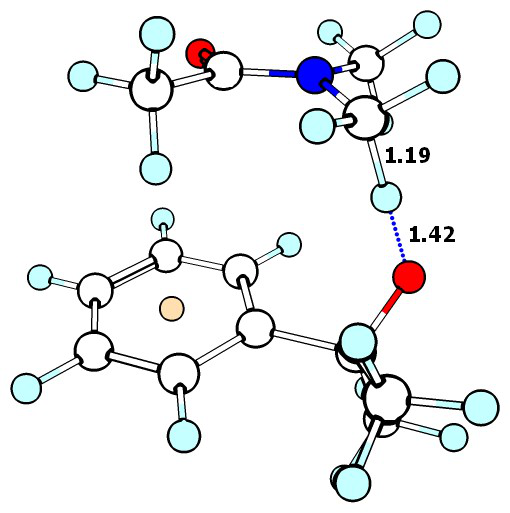
\includegraphics[width=5cm]{figures/dma-cumo-trans}
	}
  \subfigure[Trans DMA-NaCl + \cumo]{
		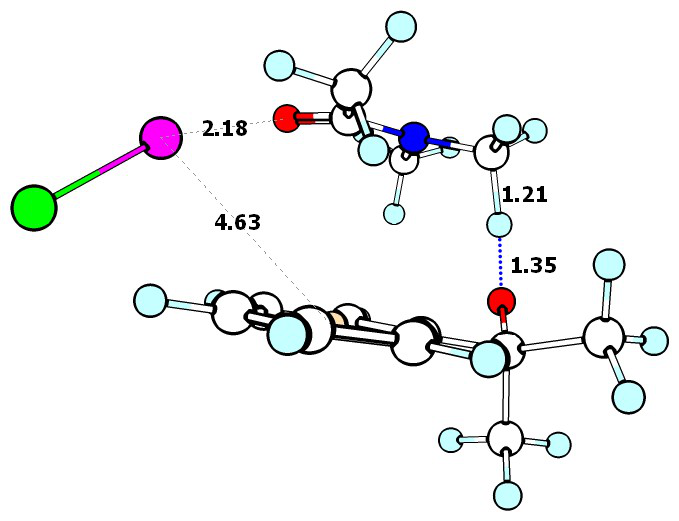
\includegraphics[width=5cm]{figures/dma-nacl-cumo-trans}
	}

  \subfigure[Cis DMA + \cumo]{
    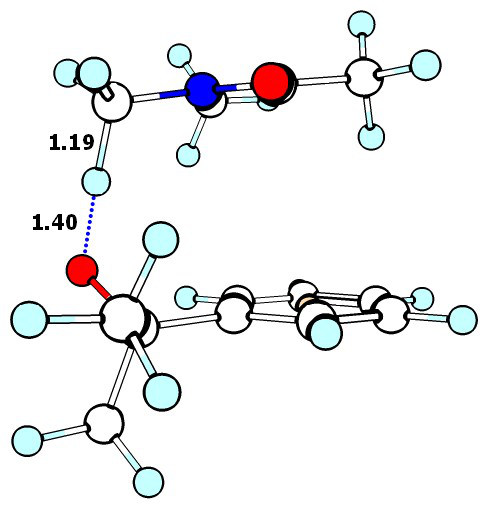
\includegraphics[width=5cm]{figures/dma-cumo-cis}
  }
  \subfigure[Cis DMA-NaCl + \cumo]{
		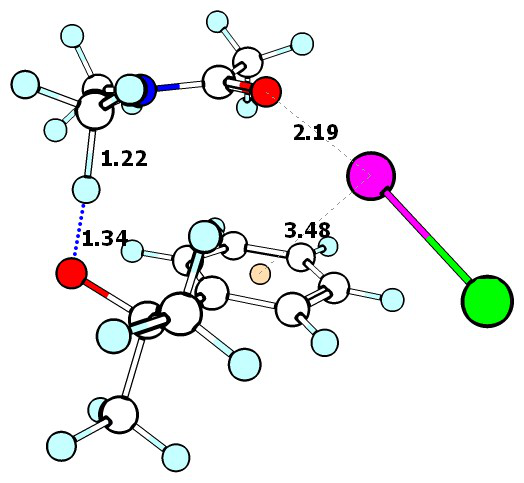
\includegraphics[width=5cm]{figures/dma-nacl-cumo-cis}
	}
  \caption[]{Continued on following page.}
\end{figure}

\begin{figure}[!htbp]\ContinuedFloat
  \setcounter{subfigure}{4}
  \subfigure[Acetyl DMA + \cumo]{
    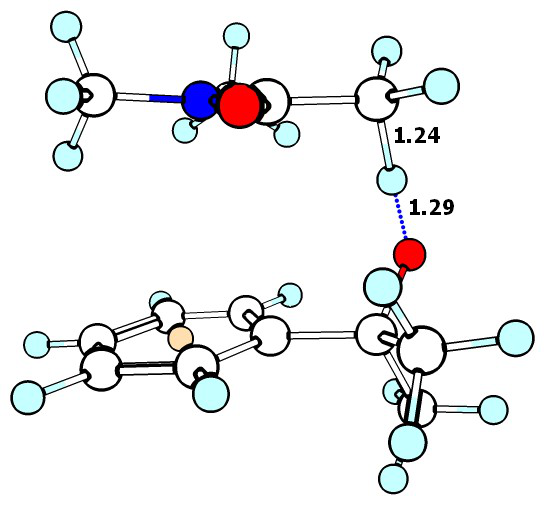
\includegraphics[width=5cm]{figures/dma-cumo-acetyl}
  }
  \subfigure[Acetyl DMA-NaCl + \cumo]{
    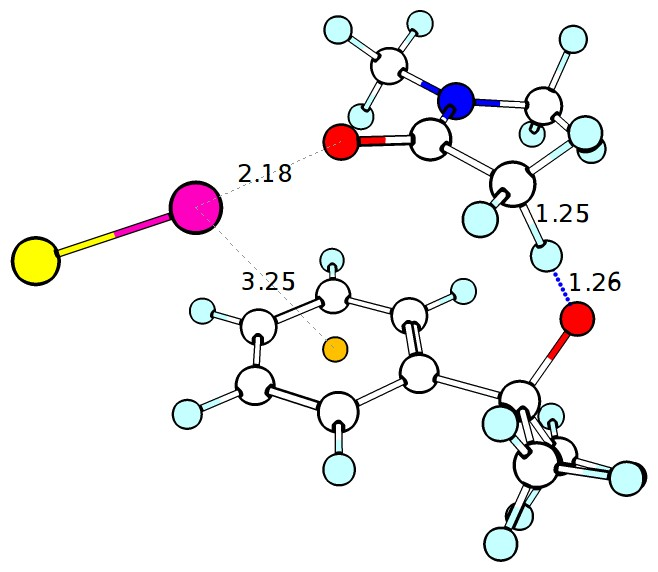
\includegraphics[width=5cm]{figures/dma-nacl-cumo-acetyl}
  }

  \caption[TS structures of HAT reaction between DMA and \cumo\ including and
  excluding NaCl.]{TS structures of HAT reaction between DMA and \cumo\
  including NaCl for different \ch{C-H} bonds: \textbf{a} trans, \textbf{b}
  trans with NaCl, \textbf{c} cis, \textbf{d} cis with NaCl, \textbf{e} acetyl,
  and \textbf{f} acetyl with NaCl. Key interatomic distances are shown in units
  of \AA. Element colour key: white is carbon, light blue is hydrogen, red is
  oxygen, blue is nitrogen, purple is sodium, green is chlorine, and peach is a
  dummy atom in the centre of an aromatic ring.}
  \label{fig:dma-cumo-ts}
\end{figure}

First, note for all the TS structures in \ref{fig:dma-cumo-ts}, the complexation
of \ch{NaCl} results in a shortening of the \ch{O-H} bond that is being formed
as a result of the HAT reaction. This indicates that the TS structure shifts
towards the product side along the reaction coordinate as a results of
interactions with \ch{NaCl}. By Hammond's postulate,\cite{Hammond1955} this
indicates a more endothermic reaction, giving evidence for increased reaction
barrier heights.

For the TS structure representing abstraction from the trans position (relative
to the carbonyl) \ch{C-H} bond of DMA by \cumo\ (\ref{fig:dma-cumo-ts}a), there
is a calculated 0.3 \kcalmol\ increase in $\Delta H^\ddagger$, which is somewhat
less than the predicted increase in BDE of 1.0 \kcalmol. This result is
consistent with the BEP principle, as the change is $\Delta H^\ddagger$ is
necessarily less than or equal to the change in $\Delta H$ due to the constant
$\alpha$ in Equation~\ref{eq:bep}. This difference can possibly be ascribed to
the effect of charge transfer: NPA indicates a 0.04 $e^-$ transfer from DMA to
\ch{NaCl}. As a result, there is less electron density available for
hyperconjugative donation to the \ch{C-H} $\sigma^*$ orbital, and thus there is
a lesser effect upon $\Delta H^\ddagger$.  Furthermore, TSs for HAT between
\ch{C-H} bond and oxygen-centred radicals are characterized by a degree of
charge separation.\cite{Roberts1999} NPA indicates that in the trans position TS
structure excluding \ch{NaCl} the charge transfer from DMA to \cumo\ is 0.24
$e^-$, but the charge transfer increases with the inclusion of \ch{NaCl} to 0.26
$e^-$. This increased charge separation results in a lower enthalpic barrier
than expected solely on the basis of the increase in \ch{C-H} BDE. While orbital
analysis does not indicate any PCET type orbital interactions, charge separation
between DMA and \cumo\ in the TS structure may be considered as a partial
ionization of the hydrogen atom. Therefore, by increasing charge separation in
the TS structure, it becomes easier to abstract the hydrogen atom as there is an
increase in the proton-transfer like character of the hydrogen atom. The
increase in $\Delta G^\ddagger$ is 3.0 \kcalmol, therefore the complexation of
metal cations increases the entropic penalty in forming the TS structure.

In the abstraction at the cis position \ch{C-H} bond of DMA by \cumo, there is a
calculated 2.6 \kcalmol\ decrease in $\Delta H^\ddagger$ and an increase of 0.9
\kcalmol\ in $\Delta G^\ddagger$. The decrease in enthalpic barrier is
inconsistent with the predicted increase in BDE of 1.8 \kcalmol\ upon
complexation with \ch{NaCl}. The TS structure in~\ref{fig:dma-cumo-ts}c shows a
possible long range interaction between \ch{Na} and the aromatic ring of \cumo\
that draws electron density and increases the reactivity. Additionally, NPA
predicts a 0.07 $e^-$ charge transfer between DMA and \ch{Na}. The combination
of these two factors stabilizes the TS and decreases $\Delta H^\ddagger$. The
entropic penalty associated with complexation of \ch{NaCl} results in an
increase in free energy barrier.

Abstraction by \cumo\ from the acetyl \ch{C-H} bond of DMA was previously
described as being a minor reaction pathway.\cite{Salamone2013} In light of the
reduction in BDE at the acetyl position of amides, it may be reasonable to
expect the reaction barrier to decrease. This indeed appears to be the net
effect of complexation of \ch{NaCl} to DMA, as $\Delta H^\ddagger$ decreases by
3.1 \kcalmol\ and $\Delta G^\ddagger$ decreases by 0.6 \kcalmol.
\ref{fig:dma-cumo-ts}f shows that in the TS structure, \ch{Na} interacts with
the aromatic system of \cumo, which also stabilizes the TS and decreases the
barrier, but not enough to make it the lowest barrier.

For HAT between DMA and \bno, the interaction between \ch{NaCl} and \bno, are
stronger as compared to \cumo, as indicated by to the shorter distance between
\ch{Na} and the centre of the aromatic ring, as shown
in~\ref{fig:dma-bno-ts}a-f. Note that, as in reactions with \cumo, the \ch{O-H}
partial bond in the TS structures are shorter upon complexation with \ch{NaCl},
indicating greater product-like character in the TS complex. This shorter
distance is likely possible due to the easier rotation of DMA relative to \bno,
as compared to \cumo. As a result, the enthalpic barriers for the abstraction
from DMA by \bno\ decrease upon complexation of \ch{NaCl} to both the acetyl and
trans position \ch{C-H} bonds. For the cis position \ch{C-H} bond of DMA
however, the enthalpic barrier increases.

This can be explained on the basis of the presence of an interaction between
\ch{Cl} and the $\alpha$-\ch{C-H} bond of \bno. While \ch{Na} withdraws electron
density from the aromatic system of \bno, \ch{Cl} is able to donate electron
density back to \bno, counteracting the effect of the interaction of \ch{Na}.
Charge analysis confirms this, such that the NPA charge on Cl in the cis
position abstraction TS complex is -0.88 $e^-$, as compared to -0.91 $e^-$ in
abstraction from the trans position. As a result, the enthalpic barrier
increases as predicted on the basis of the increase of the cis position \ch{C-H}
BDE of DMA.

\begin{figure}[!htbp]
  \setcounter{subfigure}{0}
  \centering
  \subfigure[Trans DMA + \bno]{
		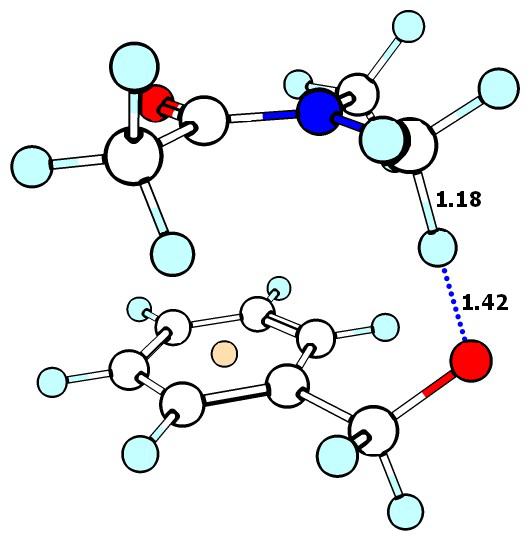
\includegraphics[width=5cm]{figures/dma-bno-trans}
	}
  \subfigure[Trans DMA-NaCl + \bno]{
		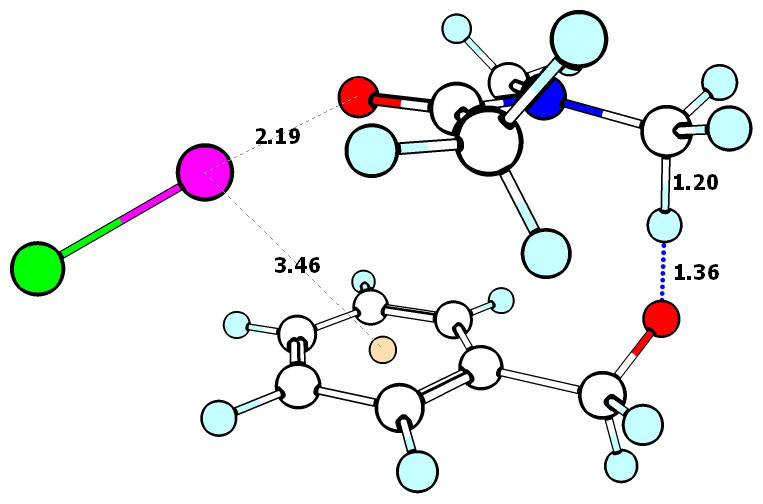
\includegraphics[width=5cm]{figures/dma-nacl-bno-trans}
	}

  \subfigure[Cis DMA+ \bno]{
		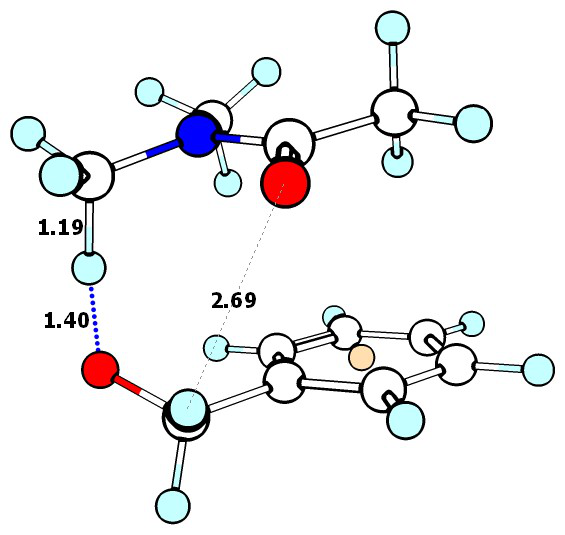
\includegraphics[width=5cm]{figures/dma-bno-cis}
	}
  \subfigure[Cis DMA-NaCl + \bno]{
		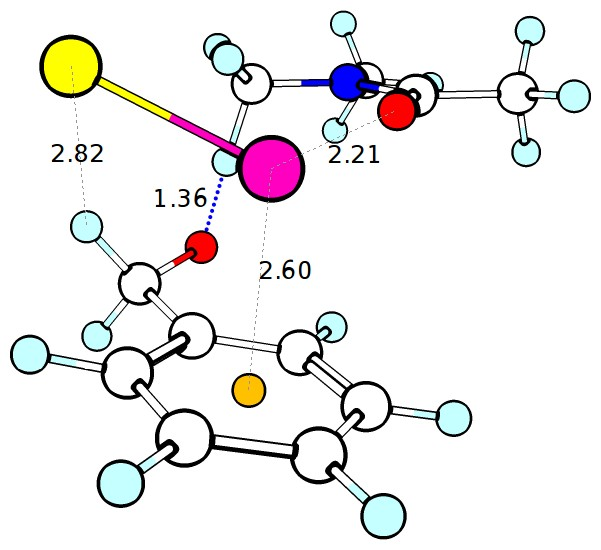
\includegraphics[width=5cm]{figures/dma-nacl-bno-cis}
	}
  \caption[]{Continued on following page.}
\end{figure}

\begin{figure}[!htbp]\ContinuedFloat
  \setcounter{subfigure}{4}
  \subfigure[Acetyl DMA + \bno]{
    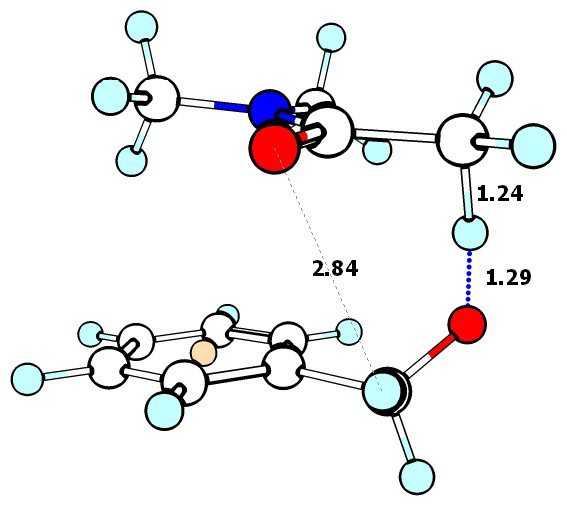
\includegraphics[width=5cm]{figures/dma-bno-acetyl}
  }
  \subfigure[Acetyl DMA-NaCl + \bno]{
    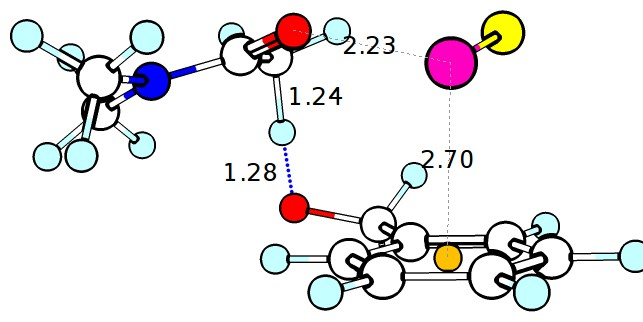
\includegraphics[width=5cm]{figures/dma-nacl-bno-acetyl}
  }

  \caption[TS structures of HAT reaction between DMA and \bno\ including
  NaCl.]{TS structures of HAT reaction between DMA and \bno\ including NaCl for
  different \ch{C-H} bonds: \textbf{a} trans, \textbf{b} trans with NaCl,
  \textbf{c} cis, \textbf{d} cis with NaCl, \textbf{e} acetyl, and \textbf{f}
  acetyl with NaCl. Key interatomic distances are shown in units of \AA.
  Element colour key: white is carbon, light blue is hydrogen, red is oxygen,
  blue is nitrogen, purple is sodium, green is chlorine, and peach is a dummy
  atom in the centre of an aromatic ring.} \label{fig:dma-bno-ts}
\end{figure}

For both \cumo\ and \bno, the presence of possible secondary interactions
between \ch{NaCl} and the radicals obfuscates the results. Therefore, in order
to determine if non-redox active metal cations may act as chemo-protective
agents in biological systems, I have performed calculated involving the more
biologically relevant \ch{HO^.} radical. Although there is no literature value
for $k_H$ of the HAT reaction between DMA and \ch{HO^.}, I have used the
Snelgrove-Ingold equation\cite{Snelgrove2001} to estimate the rate constant as
1.5\E{10} \Ms, which is two and five orders of magnitude greater than \bno\ and
\cumo, respectively. Unfortunately, I was unsuccessful in performing full
optimization calculations in the presence of the metal salt. Therefore, I have
listed these preliminary results and the analysis thereof in
Appendix~\ref{ap:hat}.


\subsection{DIA}

Next, to study the effect steric bulk has on the HAT reactions between amides
and oxygen-centred radical, I have performed a study of HAT between DIA and
\cumo. The HAT reaction between DIA and \cumo\ was previously studied by
\citet{Salamone2014}, however only the $\alpha$-N-alkyl positions were studied
theoretically. Since the BDEs for $\alpha$- and $\beta$-N-alkyl \ch{C-H}
positions are relatively close in energy, I calculated the reaction barriers
for these positions as well. The calculated free energy (enthalpic) barriers
excluding and including \ch{NaCl} are listed in ~\ref{tab:dia-cumo}.
Interestingly the predicted reaction barriers for abstraction of the
$\beta$-positions of DIA are lower than the $\alpha$-positions. By applying the
Boltzmann distribution about 69\% of abstractions by \cumo\ from DIA will take
place from either the cis- or trans-$\beta$ positions of DIA. Therefore,
abstraction from bulky amides by bulky oxygen-centred radicals are likely
controlled by steric considerations. Note also that many of the TS
optimizations were not successful with the inclusion of \ch{NaCl} and in which
case ``guess'' TS structures have been used to estimate the barrier heights.
The TS structures for the HAT reaction between DIA and \cumo\ including
\ch{NaCl} are shown in~\ref{fig:dia-cumo-ts}.

\begin{table}[!htbp]
\caption[Calculated free energy (enthalpy) for direct HAT from different
\ch{C-H} bonds in DIA by \cumo, with and without \ch{NaCl}.]{Calculated free
energy (enthalpy) ($\Delta G(H)^\ddagger$, \kcalmol) for direct HAT from
different \ch{C-H} bonds in DIA by \cumo, with and without \ch{NaCl}. The change
in barrier height ($\Delta \Delta G(H)^\ddagger$) is calculated relative to the
same abstraction site without the inclusion of \ch{NaCl}. All barrier heights
are relative to separated reactants (or complexed DIA-NaCl) and were calculated
at the M05-2X-SMD(MeCN)/6-311+G(2d,2p)//M05-2X/6-31+G$^{**}$ level of theory.
$^*$Indicates estimated barrier based on ``guess'' TS structure.}
\label{tab:dia-cumo}
  \begin{tabular}{l l c c}
    Reaction   &  Abstraction Site   &  $\Delta G(H)^\ddagger$ &  $\Delta \Delta G(H)^\ddagger$ \\
    \hline
    DIA + \cumo    &  $\alpha$-trans    &  19.5(6.2)  &              \\
                   &  $\alpha$-cis      &  19.1(5.4)  &              \\
                   &  $\beta$-trans     &  18.6(6.0)  &              \\
                   &  $\beta$-cis       &  18.4(6.5)  &              \\
                   &  acetyl         &  19.1(7.4)  &              \\
    DIA-NaCl + \cumo &  $\alpha$-trans$^*$  &  17.0(3.9)  &   -2.5(-2.3)  \\
                   &  $\alpha$-cis$^*$      &  12.7(-2.4) &   -6.4(-7.8) \\
                   &  $\beta$-trans     &  19.8(6.8)  &    0.7(1.4)  \\
                   &  $\beta$-trans$^*$     &  19.6(6.9)  &    0.5(1.5)  \\
                   &  $\beta$-cis$^*$       &  16.8(4.2)  &   -1.6(-2.3) \\
                   &  acetyl$^*$         &  17.8(3.8)  &    0.8(-0.1) \\
                   &  acetyl             &  17.9(3.7)  &    0.9(-0.2)
  \end{tabular}
\end{table}

\begin{figure}
  \setcounter{subfigure}{0}
  \centering

  \subfigure[$\alpha-$trans DIA-NaCl + \cumo]{
		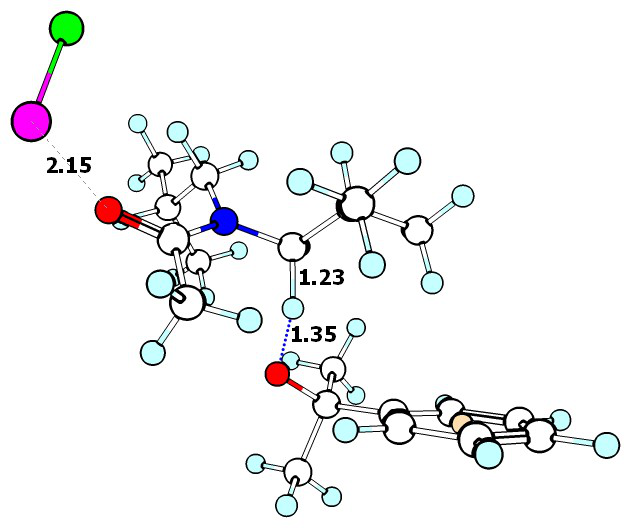
\includegraphics[width=5cm]{figures/dia-nacl-cumo-trans-alpha}
	}
  \subfigure[$\alpha-$cis DIA-NaCl + \cumo]{
		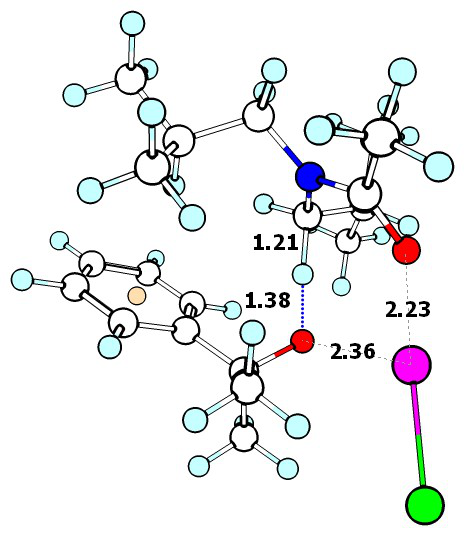
\includegraphics[width=5cm]{figures/dia-nacl-cumo-cis-alpha}
	}

  \subfigure[$\beta-$trans DIA-NaCl + \cumo]{
		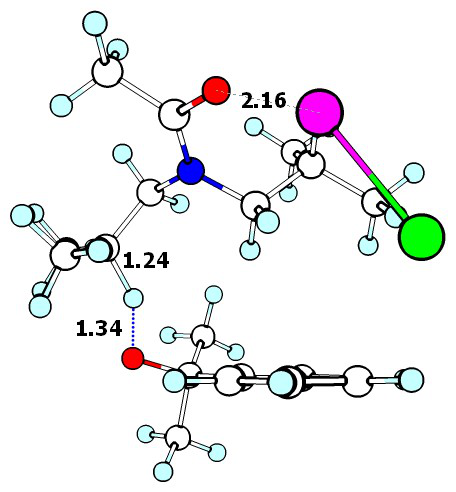
\includegraphics[width=5cm]{figures/dia-nacl-cumo-trans-beta}
	}
  \subfigure[$\beta-$cis DIA-NaCl + \cumo]{
		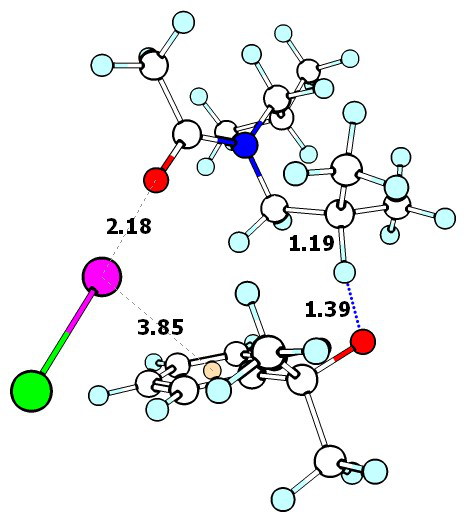
\includegraphics[width=5cm]{figures/dia-nacl-cumo-cis-beta}
	}
  \caption[]{Continued on following page.}
\end{figure}

\begin{figure}\ContinuedFloat
  \setcounter{subfigure}{4}
  \subfigure[Acetyl DIA-NaCl + \cumo]{
    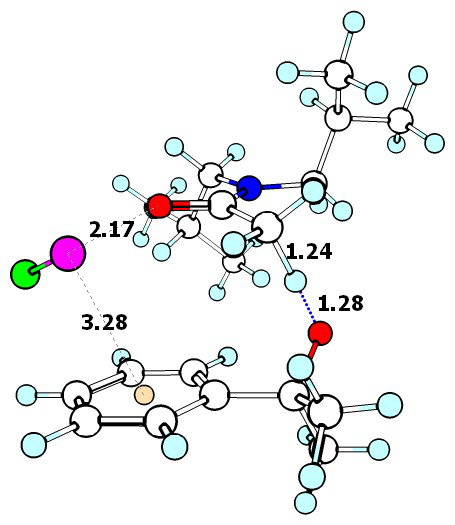
\includegraphics[width=5cm]{figures/dia-nacl-bno-acetyl}
  }

  \caption[TS structures for HAT reaction between DIA and \cumo\ including
  NaCl.]{TS structures for HAT reactions between DIA and \cumo\ including NaCl
  for different \ch{C-H} bonds: \textbf{a} $\alpha$-trans, \textbf{b}
  $\alpha$-cis, \textbf{c} $\beta$-trans, \textbf{d} $\beta$-cis, and
  \textbf{e} acetyl. Key interatomic distances are shown in units of \AA.
  Element colour key: white is carbon, light blue is hydrogen, red is oxygen,
  blue is nitrogen, purple is sodium, green is chlorine, and peach is a dummy
  atom in the centre of an aromatic ring.}
  \label{fig:dia-cumo-ts}
\end{figure}

As was observed in the barrier height calculations involving \ch{NaCl} with DMA
with \bno\ and \cumo, the results vary depending on the presence or absence of
secondary interactions of \ch{Na} with \cumo. For the $\beta$-cis and acetyl
position of DIA (\ref{fig:dia-cumo-ts}d-e), $\Delta H^\ddagger$ decreases by 2.3
and 0.2 \kcalmol, respectively, as a result of relatively long range
interactions of \ch{Na} with the aromatic system of \cumo. For abstraction from
the $\alpha$-cis position of DIA (\ref{fig:dia-cumo-ts}b), \ch{Na} is able to
interact with both the amidic oxygen lone pair, and a lone pair on the oxygen of
\cumo, resulting in a significant decrease in $\Delta H^\ddagger$ by 7.8
\kcalmol.

For the $\alpha$-trans position there is no interaction between \ch{Na} and
\cumo, however the complexation of \ch{NaCl} to DIA results in a 2.5 \kcalmol\
decrease in $\Delta G^\ddagger$. Comparing the TS structures including and
excluding NaCl, there is very little difference. Therefore, it is likely that
the ``guess'' TS structure including NaCl does not appropriately represent the
``true'' TS structure for this particular abstraction site. Note that this may
also be the case in other systems.

Abstraction by \cumo\ from the $\beta$-trans position of DIA does not allow for
an interaction between both the amidic oxygen and \cumo. However, there should
be no effect from decreased electron density in the \ch{C-H} $\sigma^*$ orbital.
Consequently, $\Delta H^\ddagger$ increases by 1.4 \kcalmol\ as a result of the
effect of 0.04 $e^-$ charge transfer from DIA to \ch{Na} in the TS structure.


\section{Summary}

In this investigation, the effects of non-redox active metal cations upon the
barrier heights of HAT reactions between small models for proteins with
oxygen-centred radicals were studied. I began by examining the effects of the
complexation of \ch{NaCl} upon the \ch{C-H} bond strengths of the substrates of
interest in this work. This in particular is central to the hypothesis of this
work: complexation of a non-redox active metal to a heteroatom of a substrate
reduces the electron density donated to adjacent \ch{C-H} $\sigma^*$ orbitals,
increasing the \ch{C-H} bond strength. By the BEP principle (See
Chapter~\ref{ch:bde}), the HAT reaction barrier height increases as a function
of the \ch{C-H} BDE.

Specific metal-substrate interactions can increase the effective \ch{C-H} BDEs
in the parent molecule, however this is complicated by the possibility for
metal-radical interactions following bond cleavage. Metal-radical interaction
can either increase or decrease \ch{C-H} BDEs depending on the nature of the
orbital interactions of the product radical and metal cation. The aforementioned
hypothesis does not take into account the effects of metal-radical interaction.

Next, I studied the effects of metal complexation on the HAT reaction barrier
heights. I calculated the barrier heights for two small models for proteins, DMA
and DIA, including and excluding \ch{NaCl}, with two different oxygen-centred
radical, \bno\ and \cumo. In the absence of any secondary interactions in the TS
complex, the enthalpic HAT reaction barrier increases as a results of metal
complexation. However, in the event of interactions between either the sodium or
chlorine moieties with the oxygen-centred radical or extensions of the substrate
in the TS complex, the effect of complexation can increase or decrease the
barrier height, depending on the specific interaction. This further motivates
the idea that the central hypothesis is incomplete in describing the effects of
non-redox active metals on HAT reaction barrier heights.

The results obtained herein do not align with those from experiment. Recall that
previous experimental results for the HAT reaction between DMA and \cumo\
demonstrated clear inhibition upon the addition of alkali and alkaline
earth-metal salts. There are several possible explanations for this discrepancy:
The models used herein may not properly capture the behaviour of bulk systems
with respect to solvation or stoichiometry (the binding of multiple amide
substrates to a single metal cation). Another possible explanation is the use of
\ch{Cl^-} as a counteranion herein, whereas \ch{ClO4^-} and \ch{OTf^-} were
utilized in experiment; the nature of the counteranion may play a larger roll
than has been previously demonstrated.

The sum of these results suggests that non-redox active metal cations may not
always deactivate \ch{C-H} bonds in complex chemical environments. Therefore, on
the basis of these limited results, it seems unlikely that a natural
chemo-protective effect is observed due to the presence of alkali and alkaline
earth-metal cations in protein or other biological systems. Additional work
should be carried out to corroborate these results.


\end{doublespace}


% !TEX root = diss.tex

\chapter{Conclusion}

\begin{doublespace}

\jnote{Currently working on.}
  
\end{doublespace}


% This file is setup to use a bibtex file sample.bib and uses the
% plain style.  Other styles may be used depending on the conventions
% of your field of study.
%
% Note: the bibliography must come before the appendices.


%change heading ``Chapter 5 Bibliography''->''Bibliography''
\newpage %newpage needed otherwise pagestyle applied to previous chapter. Does not actually create a new page
\pagestyle{fancy}\chead{References}\rhead{}\cfoot{}\rfoot{\thepage}

%Bibliography style is discipline dependent. Mathematic student can use e.g. SIAM
%\bibliographystyle{achemso}
\bibliography{\string~/Dropbox/bib/MSc}%name of your .bib file

\newpage
\pagestyle{headings}


\addtocontents{toc}{%
\protect\renewcommand*\protect\cftchappresnum{\appendixname~}}

%%\part{Appendix}

\appendix
\addappheadtotoc %uses the current page number when it makes the entry in the ToC
\appendixpage
\pagestyle{plain}

% !TEX root = diss.tex

\chapter{BDE data}

\begin{longtable}{m{3.1cm} | c c c}
\caption[Summary of experimental rate constants and literature bond dissociation enthalpies (BDEs).]{Summary of experimental rate constants and literature\cite{Luo2002} bond dissociation enthalpies (BDEs).} \label{tab:expt-bde} \\
\centering
 Molecule                       & $k_H$ \Ms          & Normalized $k_H$ \Ms & BDE \kcalmol \\
\toprule
 1,4-cyclohexadiene             & $ 6.60 \times 10^7$ & $1.65 \times 10^7 $ &        76 \\
 1,4-diazabicyclo-[2.2.2]octane  & $ 9.60 \times 10^6$ & $8.00 \times 10^5 $ &      93.4 \\
 2,2-dimethylbutane             & $ 9.50 \times 10^4$ & $4.75 \times 10^4 $ &        98 \\
 2,3-dimethylbutane             & $ 5.60 \times 10^5$ & $2.80 \times 10^5 $ &      95.4 \\
 9,10-dihydroanthracene         & $ 5.04 \times 10^7$ & $1.26 \times 10^7 $ &      76.3 \\
 Acetone                        & $ < 1 \times 10^4 $ & $2 \times 10^3    $ &        96 \\
 Acetonitrile                   & $ < 1 \times 10^4 $ & $2 \times 10^3    $ &        97 \\
 Adamantane (2$^\circ$)                & $ 6.90 \times 10^6$ & $5.75 \times 10^5 $ &      98.4 \\
 Adamantane (3$^\circ$)                & $ 6.90 \times 10^6$ & $1.73 \times 10^6 $ &      96.2 \\
 Benzaldehyde                   & $ 1.20 \times 10^7$ & $1.20 \times 10^7 $ &      88.7 \\
 Benzyl alcohol                 & $ 2.97 \times 10^6$ & $1.49 \times 10^6 $ &        79 \\
 Cumene                         & $ 5.60 \times 10^5$ & $5.60 \times 10^5 $ &      83.2 \\
 Cycloheptane                   & $ 2.20 \times 10^6$ & $1.57 \times 10^5 $ &        94 \\
 Cyclohexane                    & $ 1.10 \times 10^6$ & $9.17 \times 10^4 $ &      99.5 \\
 Cyclooctane                    & $ 2.98 \times 10^6$ & $1.86 \times 10^5 $ &      94.4 \\
 Cyclopentane                   & $ 9.54 \times 10^6$ & $9.54 \times 10^5 $ &      95.6 \\
 Dibenzyl ether                 & $ 5.60 \times 10^6$ & $1.40 \times 10^6 $ &      85.8 \\
 Diethyl ether                  & $ 2.60 \times 10^6$ & $6.50 \times 10^5 $ &        93 \\
 Dimethyl sulfoxide              & $ 1.80 \times 10^4$ & $6.00 \times 10^3 $ &        94 \\
 Dioxane                        & $ 8.20 \times 10^5$ & $1.03 \times 10^5 $ &      96.5 \\
 Diphenylmethane                & $ 8.71 \times 10^5$ & $4.36 \times 10^5 $ &      84.5 \\
 Ethylbenzene                   & $ 7.90 \times 10^5$ & $3.95 \times 10^5 $ &      85.4 \\
 Hexamethyl-phorsphoramide       & $ 1.87 \times 10^7$ & $1.04 \times 10^6 $ &           \\
 Morpholine                     & $ 5.00 \times 10^7$ & $1.25 \times 10^7 $ &        92 \\
 Piperazine                     & $ 2.4 \times 10^8 $ &                &        93 \\
 Piperidine                     & $ 1.2 \times 10^8 $ &                &      89.5 \\
 Pyrrolidine                    & $ 1.1 \times 10^8 $ &                &        89 \\
 Tetrahydro-2H-pyran            & $ 1.4 \times 10^6 $ &                &        96 \\
 Tetrahydrofuran                & $ 5.8 \times 10^6 $ &                &      92.1 \\
 Toluene                        & $ 1.85 \times 10^5$ & $6.17 \times 10^4 $ &      89.7 \\
 Triethylamine                  & $ 2.10 \times 10^8$ & $3.5 \times 10^7  $ &      90.7 \\
 Triphenylmethane               & $ 3.04 \times 10^5$ & $3.04 \times 10^5 $ &        81 \\
\end{longtable}


\begin{landscape}
%\singlespacing
\begin{longtable}{m{3.1cm} | c c c c c c c c}
\caption[Bond dissociation enthalpies of the species used to investigate the accuracy of composite methods.]{Bond dissociation enthalpies of the species used to investigate the accuracy of composite methods. All values are in \kcalmol. Statistics are listed at the bottom of the table.} \label{tab:bde-calc} \\
Molecule                         &  Lit.\cite{Luo2002}      &   W1BD   &     LDBS &     CBS-QB3 &   ROCBS-QB3 &   CBS-APNO &    G4   &    G4(MP2)\\
\hline
\endfirsthead
Molecule                         &  Lit.\cite{Luo2002}      &   W1BD   &     LDBS &     CBS-QB3 &   ROCBS-QB3 &   CBS-APNO &    G4   &    G4(MP2)\\
\hline
\endhead
1,3-pentadiene                   &  83.0     &   82.9   &   82.2   &    80.9     &    81.7    &   81.8   &  81.6   &    82.1   \\
1,4-diazabicyclo[2.2.2]-octane   &  93.4     &          &   98.9   &    98.9     &    98.8    &   98.5   &  96.7   &    95.6   \\
1,4-pentadiene                   &  76.6     &   76.2   &   76.0   &    74.2     &    75.0    &   75.2   &  75.1   &    75.7   \\
2,2-dimethylbutane               &  98.0     &   99.3   &   99.1   &    99.4     &    99.3    &   99.7   &  97.5   &    96.7   \\
2,3-dimethylbutane               &  95.4     &   97.8   &   97.7   &    97.9     &    97.8    &   98.0   &  96.2   &    95.5   \\
2-methylbutane                   &  95.8     &   97.3   &   97.2   &    97.3     &    97.1    &   97.3   &  95.9   &    95.5   \\
Acetaldehyde                     &  94.3     &   95.9   &   95.3   &    95.3     &    95.7    &   95.5   &  94.9   &    94.8   \\
Acetone                          &  96.0     &   96.9   &   96.4   &    96.2     &    96.7    &   97.1   &  95.4   &    95.0   \\
Acetonitrile                     &  97.0     &   96.9   &   96.6   &    96.2     &    96.6    &   96.5   &  96.3   &    96.3   \\
Adamantane (2$^\circ$)           &  98.4     &          &  100.9   &   100.5     &   100.4    &  100.9   &  97.8   &    96.3   \\
Adamantane (3$^\circ$)           &  96.2     &          &  100.3   &    99.9     &    99.9    &  100.3   &         &    95.7   \\
Benzaldehyde                     &  88.7     &          &   90.9   &    91.5     &    91.4    &   91.0   &  89.3   &    88.2   \\
Benzene                          & 112.9     &  113.1   &  112.7   &   115.4     &   113.0    &          &         &   113.0   \\
Benzyl Alcohol                   &  79.0     &          &   84.4   &    84.3     &    83.2    &   83.9   &  83.4   &    83.6   \\
Cumene                           &  83.2     &          &   87.9   &    87.9     &    86.9    &          &  86.9   &    86.7   \\
Cycloheptane                     &  94.0     &          &   96.0   &    96.0     &    95.8    &   96.1   &  93.9   &    92.9   \\
Cyclohexadiene                   &  76.0     &   76.3   &   76.2   &    74.3     &    75.0    &          &  75.2   &    75.5   \\
Cyclohexane                      &  99.5     &   99.2   &   99.1   &    99.4     &    99.3    &   99.6   &  97.5   &    96.8   \\
Cyclooctane                      &  94.4     &          &   92.6   &    92.6     &    92.4    &   92.8   &  90.2   &    89.1   \\
Cyclopentane                     &  95.6     &   96.3   &   96.1   &    96.5     &    96.3    &   96.6   &  95.6   &    95.0   \\
Cyclopropane                     & 106.3     &  109.0   &  108.5   &   109.3     &   109.2    &  109.5   & 108.2   &   108.0   \\
Dibenzyl ether                   &  85.8     &          &   83.6   &    84.3     &    82.7    &          &         &    79.6   \\
Diethyl ether                    &  93.0     &   95.3   &   95.1   &    95.6     &    95.5    &   95.4   &  93.8   &    93.1   \\
Dihydroanthracene                &  76.3     &          &   80.4   &    80.9     &    78.1    &          &         &    79.9   \\
Dimethylamine                    &  94.2     &   92.6   &   92.4   &    92.9     &    92.8    &   92.7   &  92.0   &    91.9   \\
Dimethylsulfoxide                &  94.0     &  102.0   &  101.7   &   102.3     &   102.3    &          & 100.9   &   100.6   \\
Dioxane                          &  96.5     &   97.3   &   97.3   &    97.7     &    97.6    &   97.4   &  95.7   &    94.9   \\
Diphenylmethane                  &  84.5     &          &   84.1   &    85.3     &    82.8    &          &         &    84.5   \\
Ethane                           & 100.5     &  101.3   &   99.3   &   101.7     &   101.5    &  101.8   & 100.7   &   100.7   \\
Ethylbenzene                     &  85.4     &          &   88.3   &    88.6     &    87.6    &   89.3   &  87.6   &    87.7   \\
Ethylene                         & 110.9     &  110.8   &  110.3   &   110.6     &   110.9    &  111.1   & 109.9   &   110.2   \\
Fluorene                         &  82.0     &          &   82.4   &    83.6     &    81.9    &          &         &    81.2   \\
Formaldehyde                     &  88.0     &   88.6   &   88.0   &    89.1     &    88.9    &   88.2   &  88.2   &    87.9   \\
Hexamethyl-phosphoramide         &           &          &   93.8   &    94.1     &    93.9    &          &         &    88.5   \\
Indene                           &  83.0     &          &   80.6   &    80.4     &    80.1    &   81.2   &  79.0   &    78.3   \\
Methane                          & 105.0     &  105.0   &  104.4   &   105.4     &   105.2    &  105.4   & 104.5   &   104.6   \\
Methanol                         &  96.1     &   96.4   &   96.0   &    96.9     &    96.8    &   96.6   &  96.0   &    95.8   \\
Methylamine                      &  93.9     &   93.1   &   92.8   &    93.4     &    93.3    &   93.3   &  92.7   &    92.8   \\
Morpholine                       &  92.0     &          &   93.4   &    93.4     &    93.3    &   93.3   &  91.8   &    91.1   \\
N,N-dimethylacetamide (acetyl)   &  91.4     &   99.6   &   99.4   &    99.5     &    99.5    &  100.1   &  97.6   &    96.8   \\
Piperazine                       &  93.0     &   93.4   &   93.5   &    93.6     &    93.5    &   93.4   &  91.9   &    91.2   \\
Piperidine                       &  89.5     &   92.1   &   92.2   &    92.3     &    92.2    &   92.1   &  90.7   &    90.0   \\
Propane                          & 100.9     &  101.6   &  101.3   &   102.0     &   101.8    &  102.1   & 100.7   &   100.4   \\
Pyrrolidine                      &  89.0     &   90.8   &   90.6   &    90.8     &    90.7    &   90.7   &  89.5   &    89.0   \\
Tetrahydro-2H-pyran              &  96.0     &   96.3   &   96.2   &    96.6     &    96.5    &   96.3   &  94.7   &    93.9   \\
Tetrahydrofuran                  &  92.1     &   93.7   &   93.3   &    93.9     &    93.8    &   93.6   &  92.2   &    91.6   \\
Toluene                          &  89.7     &   90.5   &   90.1   &    90.6     &    89.7    &   91.9   &  89.8   &    90.2   \\
Trichloromethane                 &  93.8     &   93.5   &   93.4   &    93.8     &    93.7    &          &  92.4   &    92.0   \\
Triethylamine                    &  90.7     &          &   91.4   &    91.3     &    91.2    &   91.4   &  89.4   &    88.4   \\
Trifluormethane                  & 106.4     &  107.2   &  106.6   &   107.4     &   107.4    &  106.8   & 105.8   &   105.0   \\
\hline
\textbf{Statistics}             & Lit.       &  W1BD    &    LDBS  &    CBS-QB3  &  ROCBS-QB3  &  CBS-APNO &    G4  &    G4(MP2)\\
\hline
Number of BDEs ($N$) &    49     &     33   &     50   &      50     &      50     &     40    &    43   &     50   \\
MAE (Lit.)                       &           &   0.82   &   1.60   &    1.88     &    1.64     &   1.35    &  1.21   &   1.57   \\
Max. Error                             &           &   1.59   &   2.41   &    2.63     &    3.15     &   1.85    &  4.19   &   6.23   \\
Min. Error                           &           &  -8.22   &  -8.04   &   -8.26     &   -8.25     &  -8.74    & -6.86   &  -6.58   \\
MAE (W1BD)                       &           &          &   0.22   &    0.32     &    0.18     &   0.20    &  0.70   &   0.88   \\
Max. Error                            &           &          &   2.00   &    2.01     &    1.26     &   1.08    &  2.05   &   2.84   \\
Min. Error                            &           &          &  -0.09   &   -2.37     &   -0.35     &  -1.39    &  0.37   &   0.02   \\
\end{longtable}

\end{landscape}

%%% Local Variables:
%%% mode: latex
%%% TeX-master: "diss"
%%% End:



\addtocontents{toc}{
\setlength{\cftbeforechapskip}{\cftbeforesecskip}
\setlength{\cftchapindent}{\cftsecindent}
\protect\renewcommand{\cftchapfont}{\cftsecfont}
\protect\renewcommand{\protect\cftchapdotsep}{\cftsecdotsep}
}

\end{document}
\endinput
